\documentclass{book}

\usepackage{work}
\usepackage{amssymb}
\usepackage{amsmath}
\usepackage{wasysym}
\usepackage[mathscr]{euscript}
\usepackage{hyperref}

\usepackage{hyperref}

\newcommand{\bs}[1]{\boldsymbol{#1}}
\newcommand{\rv}[1]{\bs{\mathscr{#1}}}
\newcommand{\e}[1]{\text{E}\left[#1\right]}
\newcommand{\cov}[2]{\text{cov}\left[#1,#2\right]}

\bibliographystyle{apalike}

\usepackage{geometry}
\geometry{
  top=0.5in,           
  inner=1.5in,
  outer=1.5in,
  bottom=0.5in,
  headheight=3ex,      
  headsep=2ex,         
}
\usepackage{fancyhdr}
\pagestyle{fancyplain}


\fancyhead{}
\lhead{\nouppercase{\leftmark}}
\rhead{\nouppercase{\rightmark}}
\cfoot{\fancyplain{}{\thepage}}
%\rfoot{Version: \today}

\usepackage{layout}          % display page dimensions

\DeclareMathAlphabet{\mathpzc}{OT1}{pzc}{m}{it}

%%%%%%%%%%%%%%%%%%%%%%%%%%%%%%%%%%%%%%%%%%%%%%%%%%%%%%%%%%%%%%%%%%%%%%%%%%%%%%%%%%%%%%%%%%%%%%%
%%%%%%%%%%%%%%%%%%%%%%%%%%%%%%%%%%%%%%%%%%%%%%%%%%%%%%%%%%%%%%%%%%%%%%%%%%%%%%%%%%%%%%%%%%%%%%%
%%%%%%%%%%%%%%%%%%%%%%%%%%%%%%%%%%%%%%%%%%%%%%%%%%%%%%%%%%%%%%%%%%%%%%%%%%%%%%%%%%%%%%%%%%%%%%%
%%%%%%%%%%%%%%%%%%%%%%%%%%%%%%%%%%%%%%%%%%%%%%%%%%%%%%%%%%%%%%%%%%%%%%%%%%%%%%%%%%%%%%%%%%%%%%%
\begin{document}

\coverpage{CUR: An Interpretable Alternative to Principal Components Analysis}

\tableofcontents

\addcontentsline{toc}{chapter}{Introduction}

\chapter*{Abstract}

While a very popular method in multivariate statistics principal components analysis has problems with the interpretability of its results. A proposed method of ameliorating these problems is the application of an algorithm for approximately decomposing matrices, the CUR algorithm. The purpose of this paper is an exploration of the CUR algorithm and its capacities as an alternative to principal components analysis. The intended audience for this paper is advanced undergraduate students in mathematics and statistics. The only prerequisites necessary are an introductory course in statistics and an introductory course in linear algebra. The structure of the paper is as follows. 

Chapters one and two give an in-depth introduction to the linear algebraic and statistical background necessary to understand the paper. {\bf The material in these first two chapters is not original}. Rather the results presented in these chapters are a reinterpretation of known results as presented in \cite{lay,rencher,johnson}. While not research these chapters are included because they bridge the knowledge gap from an undergraduate mathematical education. If one is comfortable with these topics already then they may proceed directly to chapter three. The third chapter is an introduction to the CUR algorithm both as it is presented in the literature and how we see its usage in place of principal components analysis. The fourth chapter consist of empirical testing of CUR on both synthetic and real data. 

After a reading of this paper we hope the readers to come away with the following knowledge.
\begin{enumerate}
\item A feeling for what the parameters of the CUR algorithm control and what reasonable rules of thumb are for choosing the parameters. 

\item Some understanding of the data on which CUR will perform relatively well or poorly in comparison to a principal components analysis. Specifically what hallmarks of the eigen-structure of the data are indicative of potential problems. 
\end{enumerate}

%%%%%%%%%%%%%%%%%%%%%%%%%%%%%%%%%%%%%%%%%%
\chapter{The Singular Value Decomposition}

The purpose of this chapter is an introduction to the singular value decomposition. The singular value decomposition (SVD) is a beautiful and unifying matrix factorization. It is one of the most useful matrix factorizations in applied linear algebra and is fundamental to the work at hand. While it is important to understand the form and mechanics of the SVD it is, in my opinion, equally as important to understand the linear algebraic geometry surrounding the SVD. In this light then this chapter will not simply be matrix algebraic proofs. Indeed it will be a discussion about linear operators and vector spaces as much as about matrices. While this may seem somewhat detached from applied statistical research progressing through the SVD in this manner is not purely a product of my own affinity for such topics. Understanding the SVD and its relation to the fundamental subspaces has direct importance to the research at hand and is thus the route this chapter will take.


\section{Diagonalization}

Our first step towards the singular value decomposition starts with the diagonalization of matrices. This topic is at the heart of the SVD. 

\subsection{Diagonal And Diagonalizable Matrices}

\subsubsection{Diagonal Matrices} An important class of matrices is the class of diagonal matrices. A diagonal matrix $A$ is a square $p \times p$ matrix for which all of the entries off the main diagonal are zero.

\ex{1}{
The following matrices $A$ and $B$ are diagonal,
$$
A=\begin{bmatrix}
1& 0&0\\
0&-5&0\\
0&0&\pi\\
\end{bmatrix}
\hspace{1cm} B=\begin{bmatrix}
1& 0\\
0& 0 
\end{bmatrix}.
$$

We will often omit the zeros and write these as
$$
A=\begin{bmatrix}
1& &\\
&-5&\\
&&\pi\\
\end{bmatrix}\text{ and }
\quad B=\begin{bmatrix}
1& & \\
 & 0&
\end{bmatrix}.
$$
}

The only parameters needed to specify a diagonal matrix are its size and its diagonal entries. Thus a diagonal matrix $D$ with diagonal entries $d_1,\ldots,d_n$ may be denoted $diag(d_1,\ldots,d_n)$. Here we assume that all of the diagonal entries are specified and so $diag(d_1,\ldots,d_n)$ is order $n$, that is, it is of size $n \times n$. 

\ex{2}{
Using the matrices $A$ and $B$ from Example $1$, 
$$
A=diag(1,-5,\pi)
$$
$$
B=diag(1,0).
$$}

There are many reasons why diagonal matrices are important in linear algebra. Indeed we will see many applications of diagonal matrices throughout this paper. For now let us consider a centrally important one: the linear transformation of a diagonal matrix. Let us  think of any real $n \times p$ matrix $A$ as describing a linear transformation $f:\mathbb{R}^p\rightarrow \mathbb{R}^n$ where 
$$
f(x) = A{\bf x} \text{ for every } {\bf x} \in \mathbb{R}^p.
$$
Since diagonal matrices are square they are a transformation on $\mathbb{R}^p$. That is, they map vectors from $\mathbb{R}^p$ into $\mathbb{R}^p$. Thus we return to the same space from whence we came. More importantly, diagonal linear transformations have very simple behavior on $\mathbb{R}^p$. They just scale the components of vectors.

For an arbitrary $p \times p$ diagonal matrix $D=diag(d_1,\ldots,d_p)$ the associated linear transformation $g:\mathbb{R}^p\rightarrow \mathbb{R}^p$ gives us a scaling. That is,  
$$
g({\bf u})=
g\left(
\begin{bmatrix}
u_1\\
\vdots\\
u_p
\end{bmatrix}
\right)=
\begin{bmatrix}
d_1& & \\
& \ddots& \\
& & d_p\\
\end{bmatrix}
\begin{bmatrix}
u_1\\
\vdots\\
u_p
\end{bmatrix}
=
\begin{bmatrix}
d_1 u_1\\
\vdots\\
d_p u_p
\end{bmatrix}\text{ for any } {\bf u}\in \mathbb{R}^p.
$$ Thus each of the components $u_i$ of {\bf u} is scaled by the $i^{th}$ diagonal entry $d_i$.  So we can think of a diagonal matrix as leaving the underlying space untouched and scaling each vector in the space by stretching or shrinking it along each direction. Alternatively we can think of such a transformation as leaving the vectors in place and stretching or shrinking the underlying space of the vectors. 

\ex{3}{
As an example consider the diagonal matrix $M=diag(3,3)$ and its associated linear transformation $T:\mathbb{R}^2\rightarrow \mathbb{R}^2$. For any ${\bf v}=(x,y)^T\in \mathbb{R}^2$ we have that 
$$
T({\bf v})=M{\bf v}=
\begin{bmatrix}
3&  \\
 & 3
\end{bmatrix}
\begin{bmatrix}
x\\
y
\end{bmatrix}=
\begin{bmatrix}
3x\\
3y
\end{bmatrix}
=3
\begin{bmatrix}
x\\
y
\end{bmatrix}=3{\bf v}.
$$
\begin{minipage}{\linewidth}
\centering%
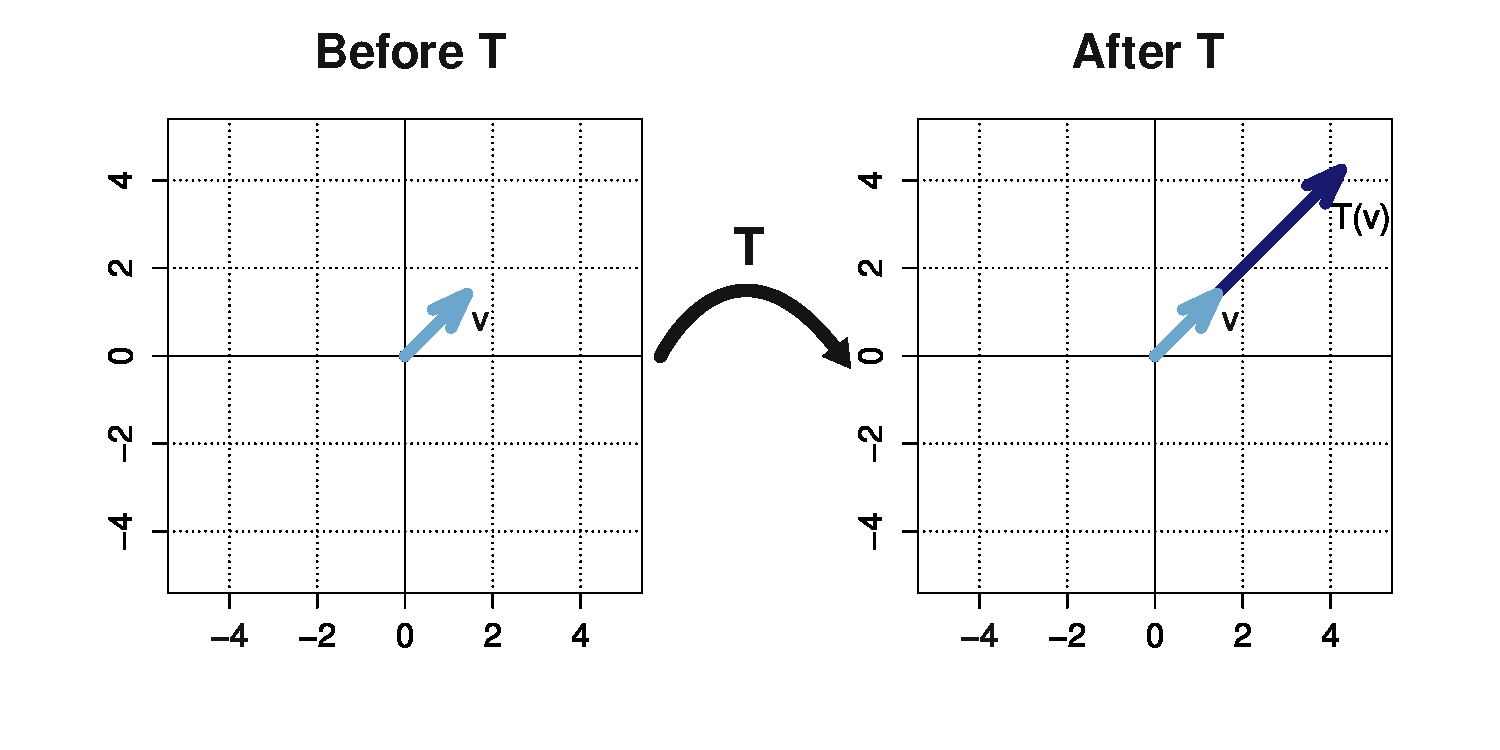
\includegraphics[scale=.35]{./Figures/F11.pdf}%
\figcaption{The map defined in Example $3$ stretches vectors by a factor of $3$.}%
\end{minipage}
}

In Example 3 the transformation $T$ just scales the vectors in $\mathbb{R}^2$ by $3$. The matrix of the transformation is $3I_2$, $I_2=diag(1,1)$ being the $2$-dimensional identity matrix. Generally 
$$
I_n=diag(\overset{n}{\overbrace{1,\ldots,1}})
$$ 
with $n$ $1's$. We will omit the subscript $n$ when the dimension is clear. The identity matrix $I_n$ is in many ways the $n$-dimensional generalization of the number $1$. Thus $3I_2$ is the two dimensional generalization of the real number $3$. So $T$ is the 2-dimensional generalization of the map $x \mapsto 3x$ for $x \in \mathbb{R}$.  Generally in the case where all of the diagonal entries are equal then a diagonal matrix represents a homogeneous scaling of the space. Here we use homogeneous to mean that each of the components is scaled by the same factor ($3$ in the above example).

\ex{4}{
Using the matrix $A$ from above and a vector ${\bf v}=(x,y,z)^T$ then the linear transformation ${\bf v} \mapsto A{\bf v}$ maps 
$$
{\bf v}=\begin{bmatrix}
x\\
y\\
z
\end{bmatrix}
\text{ into }
A{\bf v}=
\begin{bmatrix}
x\\
-5y\\
\pi z
\end{bmatrix}.
$$}

This example serves to show that not all diagonal transformations are homogeneous. One might call the transformation of Example $4$ an \emph{in}homogeneous scaling because it doesn't scale the components by the same factor. In this case it scales the components by $1,-5$ and $\pi$ respectively. Nonetheless the behavior of diagonal transformations are quite easy to understand. They simply scale each component by some value.


\subsubsection{Diagonalizing Matrices} Obviously not all square matrices are diagonal. Yet this is not to say that we can't view their associated linear transformations as scalings. Indeed the linear transformations of many $p \times p$ square matrices may be viewed as scalings of $\mathbb{R}^p$ if we look at their action through the lens of a suitably chosen basis.

Consider a linear transformation $T$ on $\mathbb{R}^p$ defined, with respect to the standard basis $\mathscr{E}$, by a $p \times p$ matrix $A$. What we would like to do is find a basis $\mathscr{B}$ such that the matrix defining $T$ under the basis $\mathscr{B}$ is diagonal. Let {\bf x} be a vector in $\mathbb{R}^p$ and assume that such a basis $\mathscr{B}$ exists. Let us define $[{\bf x}]_\mathscr{E}$ and $[{\bf x}]_\mathscr{B}$ to be the standard basis and $\mathscr{B}$ basis representations of {\bf x} respectively. Then $T$ is defined in the standard $\mathscr{E}$ basis by 
$$
[T({\bf x})]_\mathscr{E}=A[{\bf x}]_\mathscr{E}
$$
or in the $\mathscr{B}$ basis by 
$$
[T({\bf x})]_\mathscr{B}=D[{\bf x}]_\mathscr{B}.
$$
where $D$ is diagonal. This second definition allows us to view $T$ as a scaling. Instead of scaling the standard basis components of ${\bf x}$ the map $T$ scales the $\mathscr{B}$ basis components of ${\bf x}$. 

Assuming such a basis $\mathscr{B}$ exists then given a standard basis representation of a vector {\bf x}, $[{\bf x}]_\mathscr{E}$, we can compute $[T({\bf x})]_\mathscr{E}$ by the following steps. 
\begin{enumerate}
\item Convert $[{\bf x}]_\mathscr{E}$ to a $\mathscr{B}$ basis representation $[{\bf x}]_\mathscr{B}$.
\item Apply the $\mathscr{B}$ representation of $T$ by left multiplying by $D$ to get $[T({\bf x})]_\mathscr{B}$.
\item Convert $[T({\bf x})]_\mathscr{B}$ back to the $\mathscr{E}$ basis representation $[T({\bf x})]_\mathscr{E}$.
\end{enumerate}

The only thing to be explained in this process is how we switch between bases. If $B$ is the matrix whose columns are the standard basis representation of the $\mathscr{B}$ basis vectors then surely $[{\bf x}]_\mathscr{E}=B[{\bf x}]_\mathscr{B}$ since $[{\bf x}]_\mathscr{B}$ is just the vector of $\mathscr{B}$ basis coordinates to ${\bf x}$. Thus $B$ maps $[{\bf x}]_\mathscr{B}$ to $[{\bf x}]_\mathscr{E}$. Then $B^{-1}$ defines the inverse linear transformation $[{\bf x}]_\mathscr{E} \mapsto [{\bf x}]_\mathscr{B}$. We can see this because if $[{\bf x}]_\mathscr{E}=B[{\bf x}]_\mathscr{B}$ then $B^{-1}[{\bf x}]_\mathscr{E}=B^{-1}B[{\bf x}]_\mathscr{B}=[{\bf x}]_\mathscr{B}$.

\newpage Then the three steps outlined above are 
\begin{enumerate}
\item Compute $[{\bf x}]_\mathscr{B}$ as $[{\bf x}]_\mathscr{B}=B^{-1}[{\bf x}]_\mathscr{E}$.
\item Compute $[T({\bf x})]_\mathscr{B}$ as $[T({\bf x})]_\mathscr{B}=D[{\bf x}]_\mathscr{B}$.
\item Compute $[T({\bf x})]_\mathscr{E}$ as $[T({\bf x})]_\mathscr{E}=B[T({\bf x})]_\mathscr{B}$.
\end{enumerate}

Thus we have,
$$
[T({\bf x})]_\mathscr{E}=B[T({\bf x})]_\mathscr{B}=BD[{\bf x}]_\mathscr{B}=BDB^{-1}[{\bf x}]_\mathscr{E}.
$$
or, dropping the basis subscript, 
$$
T({\bf x})=BDB^{-1}{\bf x}
$$
where ${\bf x}$ is a standard basis representation of a vector in $\mathbb{R}^p$. 

Now we know that in the standard basis
$$
T({\bf x})=A{\bf x}
$$
and so it must be that
$$
A=BDB^{-1}
$$
or
$$
AB=BD
$$
and since 
$
B=
\begin{bmatrix}
{\bf b_1}& \cdots& {\bf b_p}
\end{bmatrix}$
 then
$$
A\begin{bmatrix}{\bf b_1}& \cdots& {\bf b_p}\end{bmatrix} = \begin{bmatrix}{\bf b_1}& \cdots& {\bf b_p}\end{bmatrix}D
$$
or
$$
\begin{bmatrix}A{\bf b_1}& \cdots& A{\bf b_p}\end{bmatrix} =\begin{bmatrix}d_1{\bf b_1}& \cdots& d_p{\bf b_p}\end{bmatrix}.
$$
This means that for $i=1,\ldots,p$
$$
A{\bf b_i}=d_i{\bf b_i}
$$
which is precisely an eigensystem problem. The ${\bf b_i}$ are eigenvectors and the $d_i$ are the associated eigenvalues. \vspace{.5cm}

Thus we have solved our problem completely. Consider a linear transformation $T$ defined in the standard basis by a matrix $A$. Then if there is a basis $\mathscr{B}$ under which $T$ is defined by a diagonal matrix then the ordered basis $\mathscr{B}$ is comprised of eigenvectors ${\bf v_1},\ldots,{\bf v_p}$ of $A$ and the diagonal representation of $T$ in this basis is $D=diag(\lambda_1,\ldots,\lambda_p)$ where $\lambda_i$ is the eigenvalue associated with the eigenvector ${\bf v_i}$. When such a basis exists then we say that $A$ and $D$ are similar. They are similar in the sense that they represent the same linear transformation under different bases. Furthermore we know that they are related by the relation
$$
A=BDB^{-1}
$$
which is called a similarity transformation of $D$. 

Solving for $D$ we find that
$$
D=B^{-1}AB.
$$
If such an eigenbasis for $\mathbb{R}^p$ exists then we say that $A$ is diagonalizable since we may diagonalize it via a similarity transformation. We may state this entire discussion as a theorem. 

\newpage
\thrm{1}{
{\bf A $p \times p$ matrix $A$ is diagonalizable if and only if it has an eigenbasis of $p$ linearly independent eigenvectors. In this case the diagonal matrix $D$ to which $A$ is similar is comprised of the associated eigenvalues of $A$.}\vspace{.5cm}

\emph{Proof.}\newline
$\Rightarrow$ The forward direction is a direct corollary of our above discussion. If $A$ is diagonalizable then we need $p$ linearly independent eigenvectors to form the matrix $B$. Furthermore the diagonal matrix is one consisting of the associated eigenvalues of $A$. By associated we mean that if $A$ has $p$ eigenpairs $\{({\bf v_i},\lambda_i)\}_{i=1}^{p}$ then the $i^{th}$ diagonal element of $D$ is the eigenvalue corresponding to the $i^{th}$ column of $B$, the $i^{th}$ eigenvector.

$\Leftarrow$ The reverse direction is not harder. If $A$ has $p$ linearly independent eigenvectors then construct $B$ by making the $i^{th}$ column of $B$ the $i^{th}$ eigenvector ${\bf v_i}$. Similarly construct $D=diag(\lambda_1,\ldots,\lambda_p)$. Then we know that $A{\bf v_i}=\lambda{\bf v_i}$ for $i=1,\ldots,p$ and so as above 
$$
AB=BD
$$
or  (since $B$ is a square matrix with linearly independent columns), 
$$
B^{-1}AB=D
$$
and thus $A$ is diagonalizable. }

While it is possible to lift this theorem out of the linear transformation lingo and state it simply as a theorem of matrix algebra it is important to understand the former. What the above theorem states is that if we can find an eigenbasis for the space using the eigenvectors of the matrix then the linear transformation defined by this matrix is quite simple, its just a scaling. 

A general theme to keep in mind in this chapter is the following. We would like to understand matrices. However there are a lot of them. The vector space of all matrices of size $n \times p$ is a $np$--dimensional space. If we could break down matrices (or certain classes of matrices) into the product of several very simple matrices then they would be easier to understand. If we can do this then the behavior of matrices would simply be the combined behavior of some very simple matrices. The purpose of this chapter is to see how we may do this. More on this later. For now let us close with an example. 

\ex{5}{

Consider the matrix
$$
A=
\begin{bmatrix}
5& -5\\
0& 4\\
\end{bmatrix}.
$$

The eigenvalues of this matrix are $\lambda_1=5$ and $\lambda_2=4$ and we can find two associated eigenvectors of 
$$
{\bf v_1} = 
\begin{bmatrix}
1\\
0
\end{bmatrix}
\text{ and }
{\bf v_2} =
\begin{bmatrix}
5\\
1
\end{bmatrix}.
$$

Since ${\bf v_1}$ and ${\bf v_2}$ aren't multiples of each other then they form a basis for $\mathbb{R}^2$. Then according to our above theorem we may diagonalize $A$ by a similarity transformation. Indeed if
$$
V=\begin{bmatrix}
1& 5\\
0& 1
\end{bmatrix}
\text{ then }
V^{-1}=
\begin{bmatrix}
1& -5\\
0& 1
\end{bmatrix}
$$
and
$$
V^{-1}AV=
\begin{bmatrix}
1& -5\\
0& 1
\end{bmatrix}
\begin{bmatrix}
5& -5\\
0& 4\\
\end{bmatrix}
\begin{bmatrix}
1& 5\\
0& 1
\end{bmatrix}=
\begin{bmatrix}
5& 0\\
0& 4
\end{bmatrix}.
$$

Figure 1.1 plots two unit eigenvectors ${\bf u_1}={\bf v_1}$ and ${\bf u_2}=\frac{1}{\sqrt{26}}{\bf v_2}$. What we can see is that while the eigenvectors are not colinear they are also not orthogonal. Thus while the eigenvectors of $A$ form a basis for $\mathbb{R}^2$ they don't form an orthonormal basis. We would like to determine for which matrices the eigenvectors can form not only a basis but an orthonormal one. 

\begin{minipage}{.8\linewidth}
\centering%
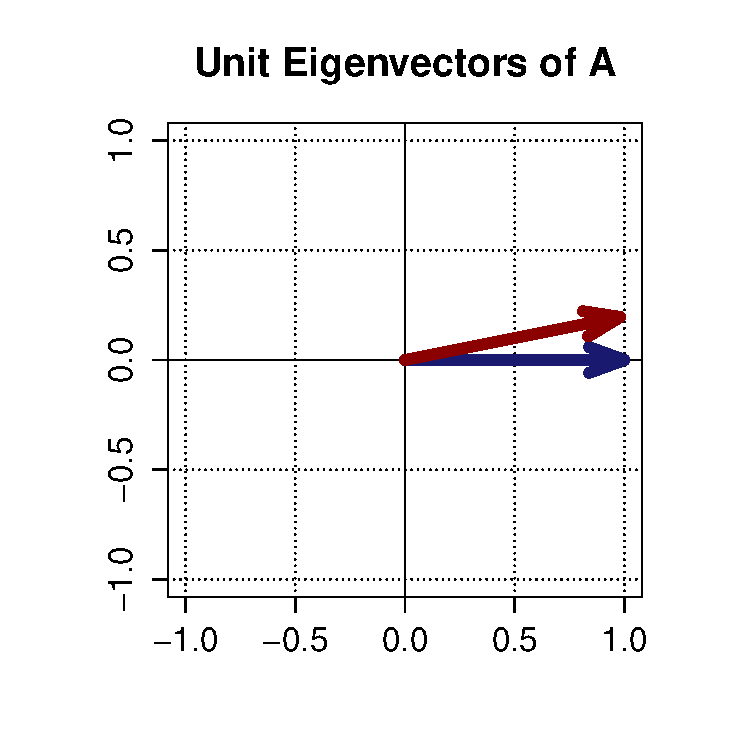
\includegraphics[scale=.5]{./Figures/F12.pdf}%
\figcaption{Blue arrow corresponds to the unit eigenvector ${\bf u_1}$ and the red line corresponds to the unit eigenvector ${\bf u_2}$.}
\end{minipage}

}

\subsection{Orthogonal Diagonalization} 

We previously discovered that many linear operators defined by a square $p \times p$ matrix may be seen as a diagonal operator on $\mathbb{R}^p$ if we use the correct basis for the space. What would be nice is if we could find an orthonormal basis for $\mathbb{R}^p$ under which a linear transformation is defined by a diagonal matrix. That will the topic of this section.

\subsubsection{Orthogonal Bases and Matrices} An orthonormal basis for a space is a basis $\mathscr{B}=\{{\bf b_1},\ldots,{\bf b_p}\}$ for which the basis vectors $\{{\bf b_i}\}$ are 
\begin{enumerate}
\item  unit vectors, meaning
$$
||{\bf b_i}||=\sqrt{{\bf b_i}^T{\bf b_i}}=1,
$$

\item mutually orthogonal such that
$$
{\bf b_i}^T{\bf b_j}=0\text{ for }i\neq j.
$$
\end{enumerate}

An orthogonal matrix $U$ (which would probably better be called an orthonormal matrix) is a $p \times p$ matrix whose columns form an orthonormal basis for $\mathbb{R}^p$. Orthogonal matrices are always full rank since their columns are linearly independent. Their inverses are quite easy to find as they are simply their transpose. Indeed the property of a matrix $U$ that
$$
U^{-1}=U^T
$$
is an alternative definition for orthogonal matrices. 

\newpage
\thrm{2}{

{\bf For a real matrix $U$, $U^{-1}=U^T$ if and only if $U$ is orthogonal.}\vspace{.5cm}

\emph{Proof.} 

$\Leftarrow$ For the reverse direction we need to show that if $U$ is orthogonal then $U^T$ is its inverse. Consider the matrix product $U^TU$. Since
$$
(U^TU)_{i,j}=row(i,U^T)\, col(j,U)=col(i,U)^T\, col(j,U)
$$
then since the columns of $U$ form an orthonormal basis distinct columns are orthogonal and so 
$$
col(i,U)^T\, col(j,U)=0 \text{ if }i \neq j
$$
and 
$$
col(i,U)^Tcol(i,U)=||col(i,U)||^2=1
$$
because the columns of $U$ are unit vectors. All together then,
$$
(U^TU)_{i,j}=
\begin{cases}
1 &\text{if } i=j\\
0 &\text{else}
\end{cases}
$$
and so $U^TU=I$. Here we are using the notation $row(i,A)$ to denote the $1\times p$ vector that is the $i^{th}$ row of $A$ and $col(j,A)$ to denote the $p \times 1$ $j^{th}$ column of $A$.

Since we can play the same game and find that $UU^T=I$ then we have that
$$
UU^T=U^TU=I
$$ 
and so $U^T$ is the inverse of $U$.

$\Rightarrow$ For the forward direction we need to show that if $U^{-1}=U^T$ then $U$ is orthogonal. This is not much different from the reverse direction. If $U^{-1}=U^T$ then 
$$
U^TU=U^{-1}U=I
$$
and so since 
$$
(U^TU)_{i,j}=row(i,U^T)\, col(j,U)=col(i,U)^Tcol(j,U)
$$
then
$$
col(i,U)^T col(j,U)=
\begin{cases}
1& \text{ if }i=j\\
0& \text{ if $i \neq j$}
\end{cases}
$$
and so all distinct pairs of the columns are orthogonal since their inner product is zero. Furthermore all of the columns are unit vectors since 
$$
col(i,U)^T col(i,U)=||col(i,U)||^2=1
$$
meaning that
$$
||col(i,U)||=1.
$$

These two conditions give us that $U$ is then orthogonal because the columns of $U$ are mutually orthogonal and unit vectors. 
}

A direct corollary from this discussion is that the transpose (or equivalently inverse) of an orthogonal matrix is orthogonal. If $U$ is orthogonal then the inverse of $U^T$ is $U=(U^T)^T$ and so the inverse of $U^T$ is its transpose and hence $U^T$ is orthogonal. 

Furthermore for an orthogonal matrix $U$, $det(U)=\pm 1$.

\newpage
\coro{}{
{\bf For $U$, an orthogonal matrix, $det(U)=\pm 1$.}\vspace{.5cm}

\emph{Proof.} Clearly
$$
det(U^{-1})=det(U^T)=\frac{1}{det(U)}
$$
but surely $det(A)=det(A^T)$ for any real matrix $A$ and so 
$$
det(U)=\frac{1}{det(U)}
$$
meaning that $det(U)$ is its own multiplicative inverse and hence $det(U)=\pm 1$.}

Now since the columns of a $p \times p$ orthogonal matrix $U$ form a basis for $\mathbb{R}^p$ then the linear transformation of an orthogonal matrix is a change of basis. However because the basis defined by the columns is orthonormal an orthogonal matrix is a particularly nice change of basis. An orthogonal matrix is simply a rotation, reflection or some rotation/reflection of the standard basis vectors. While we won't go into a formal proof of this we would like to point out the more important point which is that an orthogonal linear transformation preserves inner product.

\thrm{3}{

{\bf Orthogonal linear transformations preserve inner product}\vspace{.5cm}

\emph{Proof.} Let ${\bf x}$ and ${\bf y}$ be vectors in $\mathbb{R}^p$ and for some orthogonal matrix $U$ let 
$$
{\bf x}_U=U{\bf x}
$$
and
$$
{\bf y}_U=U{\bf y}
$$
be the images of {\bf x} and {\bf y} under the linear transformation defined by $U$. Then 
$$
{\bf x}_U^T{\bf y}_U=(U{\bf x})^T(U{\bf y})={\bf x}^TU^TU{\bf y}={\bf x}^T{\bf y}
$$
since $UU^T=I$.}


Since inner product is preserved then vector norms are preserved. Thus the length of vectors is preserved under orthogonal matrices as well as the distance between vectors. After all the distance between vectors is simply
$$
dist(u,v)=||u-v||
$$
for $u,v \in \mathbb{R}^p$. Thus the distances of all vectors from the origin (their norms) and the distance between all vectors are unchanged under orthogonal linear transformations. So the geometry of the space is really unchanged under the transformation. What has changed is that the vectors are expressed in a different basis. While non-orthogonal linear transformations will stretch or collapse the space orthogonal transformations do not do this. If we imagine a vector space as some kind of Euclidean space with points representing the vectors, then an orthogonal transformation simply removes one coordinate system and replaces it with a new (yet still orthonormal) system. Alternatively we can think of leaving the underlying space alone and rotating (really roto-inverting) all of the vectors in the space. 

\newpage
\ex{6}{
The $p \times p$ identity matrix $I_p$ is an orthogonal matrix because $I^{-1}=I^T=I$. Furthermore the $2 \times 2$ rotation matrix of the plane $\mathbb{R}^2$ through an angle $\theta$,
$$
R=\begin{bmatrix}
\cos(\theta)& -\sin(\theta)\\
\sin(\theta)& \cos(\theta)
\end{bmatrix}
$$
is an orthogonal matrix. We can see this because the columns are orthogonal since
$$
\begin{bmatrix}
\cos(\theta)& \sin(\theta)\\
\end{bmatrix}
\begin{bmatrix}
-\sin(\theta)\\
\cos(\theta)
\end{bmatrix}=
-\cos(\theta)\sin(\theta)+\sin(\theta)\cos(\theta)=0
$$
and the columns are unit vectors because
$$||col(1,R)||=||col(2,R)||=\sqrt{cos^2(\theta)+\sin^2(\theta)}=1.$$

\begin{minipage}{.8\linewidth}
\centering%
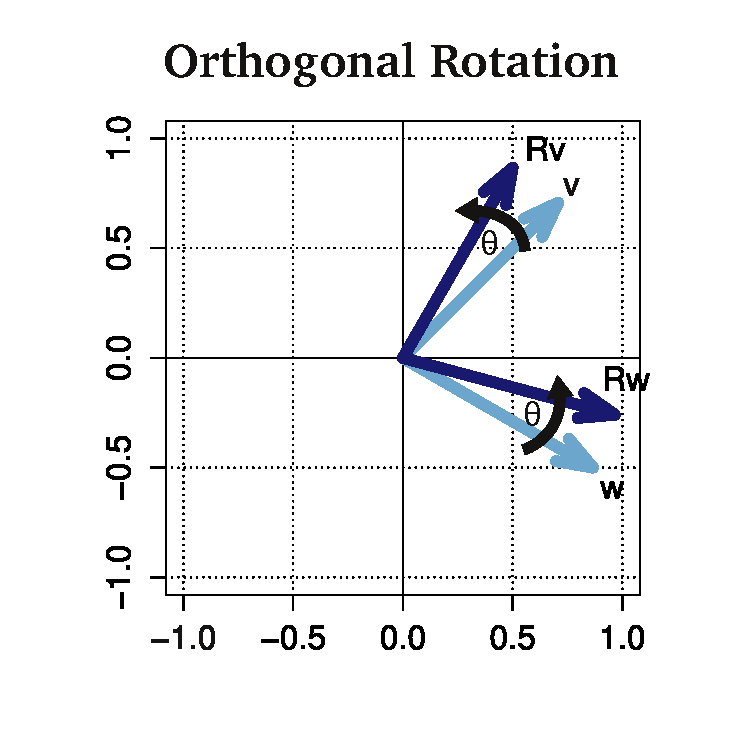
\includegraphics[scale=.5]{./Figures/F13.pdf}%
\figcaption{The rotation matrix in Example 6 rotates all of the vectors in the space through some angle $\theta$. Notice that the distances between all vectors remain unchanged under the transformation by the matrix $R$.}
\end{minipage}
}

\subsubsection{Orthogonal Diagonalization}Now Theorem 1 told us that if a $p \times p$ matrix $A$ had an eigenbasis for $\mathbb{R}^p$ then we could diagonalize $A$ via a similarity transformation $B^{-1}AB$ such that
$$
D=B^{-1}AB
$$
where the columns of $B$ are an eigenbasis for $\mathbb{R}^p$ and the diagonal entries of $D$ are the corresponding eigenvalues. What we would like to find out is when we can diagonalize a matrix $A$ via an orthogonal similarity transformation such that
$$
D=U^{-1}AU=U^TAU
$$
where $U$ is an orthogonal matrix and so $U^{-1}=U^T$. If we can do this then the linear transformation of the matrix $A$ may be seen as a scaling under the appropriate roto-inversion of the space. 

\newpage
The first thing that we must notice is that if a matrix $A$ is orthogonally diagonalizable, that is
$$
D=U^TAU
$$
then
$$
A=UDU^T
$$
and so 
$$
A^T=(UDU^T)^T=(U^T)^TD^TU^T=UDU^T=A
$$
and so $A$ must be symmetric (meaning $A=A^T$). It turns out that this is enough, a matrix is orthogonally diagonalizable if and only if it is symmetric. 

To prove this we will need the following fact. While only symmetric matrices are orthogonally diagonalizable by a similarity transformation a wider class of real matrices are orthogonally triangulable by an orthogonal similarity transformation.

\thrm{4}{

{\bf A $p \times p$ real matrix $A$ is similar (via an orthogonal similarity transformation) to a upper triangular matrix $\mathscr{T}$ if $A$ has $p$ (counting multiplicities) real eigenvalues.}\vspace{.5cm}

\emph{Proof.} This factorization is known as the Schur factorization. We will prove it by induction on the order of the matrix. 

Vacuously this is true for a $1 \times 1$ matrix (really just a scalar). Now assume it is true for all matrices of order $n-1$, i.e. square $(n-1)\times (n-1)$ matrices, such that all order $n-1$ matrices with $n-1$ real eigenvalues are similar via an orthogonal similarity transformation to an upper triangular matrix. 

Consider an $n \times n$ matrix $A$ with $n$ real eigenvalues. Let $\mu$ be an eigenvalue and pick an associated unit eigenvector ${\bf u}$. Now find vectors ${\bf w_2},\ldots,{\bf w_n}$ (via Gram-Schmidt or the like) such that $\{{\bf u},{\bf w_2},\ldots,{\bf w_{n}}\}$ is an ordered orthonormal basis for $\mathbb{R}^n$. Let $U$ be the matrix which has ${\bf u},{\bf w_2},\ldots,{\bf w_n}$ as its columns. Then 
\begin{align}
U^TAU&=U^T\begin{bmatrix}
A{\bf u}& A{\bf w_2}& \cdots& A{\bf w_{n}}\\
\end{bmatrix}\notag\\
&=
U^T\begin{bmatrix}
\mu{\bf u}& *& \cdots& *\\
\end{bmatrix}\notag\\
&=
\left[
\begin{array}{c|c}
  \mu{\bf u}^T{\bf u} & * \cdots * \\ \hline
  0 & \raisebox{-15pt}{{\huge\mbox{{$C$}}}} \\[-4ex]
  \vdots & \\[-0.5ex]
  0 &
\end{array}
\right]
=
\left[
\begin{array}{c|c}
  \mu& *\\ \hline
  0 & C
\end{array}
\right]\notag
\end{align}
where $C$ is the corner $(n-1)\times (n-1)$ block of the matrix and the $*'s$ indicate entries whose values we do not particularly care about. Now $det(U)=det(U^T)=\pm 1$ since $U$ is orthogonal and so for some scalar $\lambda$, 
\begin{align}
det(A-\lambda I)&=det(U^T)det(A-\lambda I)det(U)\notag\\
&=det(U^T(A-\lambda I)U)\notag\\
&=det(U^TAU-U^TU\lambda I)\notag\\
&=det(U^TAU-\lambda I)\notag
\end{align}
and so the characteristic equation for $U^TAU$ is the same as that for $A$ meaning they share the same eigenvalues. 

We can use the row operations of row interchange or row addition to manipulate the $C-\lambda I$  block of $U^TAU-\lambda I$ into an upper triangular matrix $(C-\lambda I)'$. That is, since 
$$
U^TAU-\lambda I=\left[
\begin{array}{c|c}
  \mu-\lambda& *\\ \hline
  0 & C-\lambda I
\end{array}
\right]
$$
then via row operations
$$
U^TAU-\lambda I\rightsquigarrow M
$$
where
$$
M=
\left[
\begin{array}{c|c}
  \mu-\lambda& *\\ \hline
  0 & (C-\lambda I)'
\end{array}
\right]
$$
and $(C-\lambda I)'$ is upper triangular. Here we use $A\rightsquigarrow B$ to denote that $A$ is transformable via row operations to $B$. 


Notice that we can do this without touching the first row of $U^TAU-\lambda I$. Furthermore since row addition doesn't change the determinant of a matrix and row interchange only flips the determinant's sign (and these are the only operations we need to use) then 
$$
det(U^TAU-\lambda I)=\pm det(M)
$$
and so the characteristic equation for the two are the same since if 
$$
det(U^TAU-\lambda I)=0
$$
then
$$
\pm det(M)=0
$$
but we can simply drop the $\pm$ and so $det(M)=0$. 

However $M$ is an upper triangular matrix and so its determinant is simply the product of its main diagonal. Since the only diagonal entry of $M$ not in $(C-\lambda I)'$ is $\mu -\lambda$ then 
$$
det(M)=(\mu-\lambda)det((C-\lambda I)')=\pm (\mu-\lambda)det(C-\lambda I)
$$
since when row reducing $U^TAU-\lambda I$ into $M$ we use only use row addition and row interchange to manipulate the submatrices
$$
C-\lambda I \rightsquigarrow (C-\lambda I)'.
$$
Thus the characteristic polynomial defined by $M$ is 
$$
\pm (\mu - \lambda)det(C-\lambda I)
$$
which has the same roots of the characteristic polynomial for $U^TAU$ and hence $A$. So if $\mu=\mu_1,\mu_2\ldots,\mu_n$ are the $n$ real eigenvalues of $A$ then $\mu_2,\ldots,\mu_n$ must be roots of $$det(C-\lambda I)=0$$ and hence $C$ has $n-1$ real eigenvalues. \vspace{.5cm}

Thus we have discovered that $C$ is a real $(n-1)\times (n-1)$ matrix with $n-1$ real eigenvalues and hence by our induction hypothesis there is some orthogonal matrix $\mathscr{O}$ such that
$$
\mathscr{O}^TC\mathscr{O}=R
$$
where $R$ is an upper triangular matrix. Then if 
$$
S=
\left[
\begin{array}{c|c}
  1& 0\\ \hline
  0& \mathscr{O} 
\end{array}
\right]
$$
it is easy to verify that
$$
\begin{aligned}
S^TU^TAUS&=
\left[
\begin{array}{c|c}
  1& 0\\ \hline
  0& \mathscr{O}^T 
\end{array}
\right]
\left[
\begin{array}{c|c}
  \mu& *\\ \hline
  0& C
\end{array}
\right]
\left[
\begin{array}{c|c}
  1& 0\\ \hline
  0& \mathscr{O}
\end{array}
\right]\notag\\
&=
\left[
\begin{array}{c|c}
  \mu& *\\ \hline
  0& \mathscr{O}^TC
\end{array}
\right]
\left[
\begin{array}{c|c}
  1& 0\\ \hline
  0& \mathscr{O}
\end{array}
\right]\notag\\
&=
\left[
\begin{array}{c|c}
  \mu& *\\ \hline
  0& \mathscr{O}^TC\mathscr{O}
\end{array}
\right]\notag\\
&=
\left[
\begin{array}{c|c}
  \mu& *\\ \hline
  0& R
\end{array}
\right].
\end{aligned}
$$
Thus if $V=US$ then $V^{-1}=(US)^{-1}=S^{-1}U^{-1}=S^TU^T=(US)^T$ and so $V$ is orthogonal and 
$$
V^TAV=S^TU^TASU=
\left[
\begin{array}{c|c}
  \mu& *\\ \hline
  0& R
\end{array}
\right]
$$
which is upper triangular since $R$ is upper triangular. Thus we have found an orthogonal matrix $V$ such that
$V^TAV$ is upper triangular. 
}

This factorization is more useful in theory than in practice. For our purposes we will prove that every $p \times p$ symmetric matrix has $p$ real eigenvalues and hence permits such a factorization. 

\thrm{5}{

{\bf The eigenvalues of a real symmetric matrix are real.}\vspace{.5cm}

\emph{Proof.} Consider a real symmetric matrix $A$ and an eigenpair $({\bf v},\lambda)$. Now we know that
$$
A{\bf v}=\lambda{\bf v}.
$$
Consider the operation of conjugate transpose for a matrix $B$ over the complex field $\mathbb{C}$. The conjugate transpose of $B$, denoted $B^{\dagger}$, is precisely as it sounds,
$$
B^{\dagger}=\overline{B}^T
$$
where $\overline{B}$ is the element-wise complex conjugate of $B$. Let us take the conjugate transpose of our first equation. Then 
$$
(A{\bf v})^\dagger=(\lambda{\bf v})^{\dagger}
$$
implies
$$
{\bf v}^\dagger A=\overline{\lambda}{\bf v}^\dagger
$$
since $A$ is real and symmetric so
$$
A^\dagger=\overline{A}^T=\overline{A}=A
$$
and $\lambda$ is a scalar so 
$$
\lambda^\dagger=\overline{\lambda}^T=\overline{\lambda}.
$$

Now consider multiplying on the right by ${\bf v}$. Then
$$
{\bf v}^\dagger A{\bf v}=\overline{\lambda}{\bf v}^\dagger{\bf v}
$$
and since $A{\bf v}=\lambda {\bf v}$ then
$$
{\bf v}^\dagger \lambda {\bf v}=\overline{\lambda}{\bf v}^\dagger{\bf v}
$$
or because $\lambda$ is a scalar and hence commutes,
$$
\lambda{\bf v}^\dagger{\bf v}=\overline{\lambda}{\bf v}^\dagger{\bf v}
$$
meaning that 
$$
\lambda = \overline{\lambda}
$$
since ${\bf v}\neq0$ because it is an eigenvector. Hence it must be that $\lambda$ is real. 
}

Since every $p \times p$ matrix has (counting multiplicities) $p$ eigenvalues over the complex field then a symmetric $p \times p$ matrix not only has all real eigenvalues it must have $p$ real eigenvalues and thus permits a Schur Factorization. This is enough to prove the main theorem of this section. 

\newpage
\thrm{6}{

  {\bf A matrix $A$ is orthogonally diagonalizable if and only if $A$ is symmetric.}\vspace{.5cm}

\emph{Proof.}

$\Rightarrow$ We have already shown that if a matrix $A$ is orthogonally diagonalizable then it must be symmetric since
$$
A^T=(UDU^T)^T=(U^T)^TD^TU^T=UDU^T=A.
$$

$\Leftarrow$ Now if a $p \times p$ matrix $A$ is symmetric then $A$ has $p$ real eigenvalues and so it has a Schur factorization such that $A$ is similar via an orthogonal similarity transformation, $\mathscr{O}$, to an upper triangular $\mathscr{T}$ as
$$
\mathscr{O}^TA\mathscr{O}=\mathscr{T}.
$$
Then $\mathscr{T}^T=(\mathscr{O}^TA\mathscr{O})^T=\mathscr{O}^TA^T(\mathscr{O}^T)^T=\mathscr{O}^TA\mathscr{O}=\mathscr{T}$ and so $\mathscr{T}$ is a symmetric triangular matrix and so it must be diagonal. 

}

Thus we have completely characterized those matrices permitting orthogonal diagonalizations. The action of any real symmetric matrix may be seen as the product of orthogonal and diagonal matrices. Such a view of symmetric matrices is quite nice. The linear transformation defined by these matrices may be viewed as simply a scaling. We can see this if we abandon the standard basis and literally rotate our viewpoint. On the other hand diagonal and orthogonal matrices are quite simple to manipulate with matrix algebra and so expressing symmetric matrices as such can simplify matrix algebraic manipulations. 

However we also see that only a very narrow family, those symmetric matrices, permit orthogonal diagonalizations. It would be nice if we could extend such ideas to a wider class of matrices. The singular value decomposition is precisely this idea. It is a matrix factorization which, as close as possible, allows orthogonal diagonalization for any arbitrary $n \times p$ matrix. 

To close this section and transition into the singular value decomposition let us consider the following example.

\ex{7}{

While any real $n \times p$ matrix $A$ is not necessarily symmetric the associated matrices $A^TA$ and $AA^T$ are symmetric since
$$
(A^TA)^T=A^T(A^T)^T=A^TA
$$
and
$$
(AA^T)^T=(A^T)^TA^T=AA^T.
$$

For example consider the real matrix
$$
A=
\begin{bmatrix}
4& 8\\
11& 7\\
14& -2
\end{bmatrix}.
$$

Then 
$$
A^TA=
\begin{bmatrix}
333& 81\\
81& 117
\end{bmatrix}
$$
and
$$
AA^T=\begin{bmatrix}
80& 100& 40\\
100& 170& 140\\
40& 140& 200
\end{bmatrix}.
$$
Now both of these matrices are symmetric and so they are orthogonally diagonalizable by our previous theorem. 

For $A^TA$ we find that the eigenvalues are $\lambda_1=360$ and $\lambda_2=90$ with associated eigenvectors of 
$$
v_1=\begin{bmatrix}
81\\
27
\end{bmatrix}
\text{ and }
v_2=\begin{bmatrix}
-27\\
81
\end{bmatrix}
$$
and so if 
$$
V=\begin{bmatrix} 
81& -27\\
27& 81
\end{bmatrix}
$$
then
$$
V^TA^TAV=diag(360,90).
$$

For $AA^T$ we find that the eigenvalues are $\mu_1=360,\mu_2=90$ and $\mu_3=0$ with associated eigenvectors of 
$$
u_1=\begin{bmatrix}
1\\2\\2
\end{bmatrix}
\text{, }
u_2=\begin{bmatrix}
2\\1\\-2
\end{bmatrix}
\text{ and }
u_3=\begin{bmatrix}
-2\\2\\1
\end{bmatrix}
$$
and so if
$$
U=\begin{bmatrix}
1& 2& -2\\
2& 1& 2\\
2& -2& -1
\end{bmatrix}
$$
then
$$
U^TAA^TU=diag(360,90,0).
$$
Notice that both $U$ and $V$ are orthogonal and so we have indeed orthogonally diagonalized these matrices. 
}

\section{The Singular Value Decomposition}

An interesting fact about Example $7$ is that the nonzero eigenvalues of $A^TA$ and $AA^T$ are equal. This is not contrived but always true. We will see that the symmetric forms $A^TA$ and $AA^T$ tell us very important information about the matrix $A$ and will thus be fundamental in developing the singular value decomposition. 

The singular value decomposition is a factorization of a real $n \times p$ matrix $A$ as 
$$
A=U\Sigma V^T
$$
where $U$ is an $n \times n$ orthogonal matrix, $V$ is a $p \times p$ orthogonal matrix and $\Sigma$ is an $n \times p$ matrix whose elements off the main diagonal are zero. 

This should look very reminiscent of the orthogonal diagonalizations of the previous section. While only symmetric matrices permit an orthogonal diagonalization \emph{any} $n \times p$ real matrix $A$ has a singular value decomposition. With symmetric matrices we may diagonalize them by a similarity transformation of a single orthogonal matrix. With any real $n \times p$ matrix we may transform it into a ``basically'' diagonal matrix $\Sigma$ with two orthogonal matrices. By basically diagonal we mean that $\Sigma$ is zero off the main diagonal but not necessarily square.  We will call such matrices ``rectangular diagonal matrices''. Thus we may rectangularly diagonalize any real $n \times p$ matrix via two orthogonal matrices $U$ and $V$ as
$$
U^TAV=\Sigma. 
$$

We notice that since $A=U\Sigma V^T$ then 
$$
A^TA=(U\Sigma V^T)^T(U\Sigma V^T)=V\Sigma^T U^TU\Sigma V^T=V(\Sigma^T\Sigma)V^T
$$
and
$$
AA^T=(U\Sigma V^T)(U\Sigma V^T)^T=U\Sigma V^TV\Sigma^T U^T=U(\Sigma \Sigma^T)U^T.
$$

Then the matrix $V$ is the matrix which orthogonally diagonalizes the symmetric form $A^TA$ and the matrix $U$ is the matrix orthogonally diagonalizing $AA^T$. Furthermore the $\Sigma$ matrix is related to the diagonalized forms of $A^TA$ and $AA^T$ and thus their respective eigenvalues. 

\subsection{The Symmetric Forms $A^TA$ and $AA^T$}

\subsubsection{Singular Values}

While the above is not a proof of the existence of the SVD it shows us some properties that must be true should such a factorization exist. In this light then it seems appropriate to investigate the symmetric forms $A^TA$ and $AA^T$. We will start by proving as a theorem the curiosity we noticed in Example 7. 

\thrm{7}{

{\bf For a real matrix $A$ the non-zero eigenvalues of $A^TA$ and $AA^T$ are the same.}\vspace{.5cm}

\emph{Proof.} Consider an eigenpair $({\bf v},\lambda)$ of $A^TA$ such that $\lambda \neq 0$. Then
$$
A^TA{\bf v}=\lambda{\bf v}
$$
left-multiplying by $A$ we get
$$
AA^TA{\bf v}=\lambda A{\bf v}
$$
or, adding parentheses for emphasis, 
$$
AA^T(A{\bf v})=\lambda (A{\bf v})
$$
where $A{\bf v}$ is an eigenvector of $AA^T$ and hence $\lambda$ is an eigenvalue of $AA^T$. We can do the same thing for $AA^T$ and show that all non-zero eigenvalues of $AA^T$ are eigenvalues of $A^TA$. Thus the set of non-zero eigenvalues is shared between the two symmetric forms. 

The thing to check, however, is that these symmetric forms not only have the same set of nonzero eigenvalues but have the same number of repetitions of nonzero eigenvalues. That is, we want to check the algebraic and geometric multiplicities of the shared non-zero eigenvalues. 

Since $A^TA$ and $AA^T$ are symmetric matrices then we know that if an eigenvalue has an algebraic multiplicity of $k$ then we can find $k$ orthogonal (not just linearly independent) eigenvectors. This follows from the fact that these matrices are orthogonally diagonalizable and thus there must be an orthonormal eigenbasis. A corollary is that the geometric multiplicity equals the algebraic. Thus let us assume that ${\bf u}$ and ${\bf v}$ are orthogonal eigenvectors corresponding to the eigenspace of an eigenvalue $\lambda$ of $A^TA$. Then
$$
A^TA{\bf u}=\lambda{\bf u}\text{ and } A^TA{\bf v}=\lambda{\bf v}
$$
and as above
$$
AA^TA{\bf u}=\lambda A{\bf u}\text{ and } AA^TA{\bf v}=\lambda A{\bf v}
$$
meaning
$$
A{\bf u}\text{ and }A{\bf v}
$$
are eigenvectors of $AA^T$ corresponding to the eigenvalue $\lambda$. Then 
$$
(A{\bf u})^T(A{\bf v})={\bf u}^TA^TA{\bf v}=\lambda {\bf u}^T{\bf v}
$$
since ${\bf v}$ is an eigenvector of $A^TA$. However since {\bf u} and {\bf v} are orthogonal then ${\bf u}^T{\bf v}=0$ and hence
$$
\lambda {\bf u}^T{\bf v}=0
$$
and so $A{\bf v}$ and $A{\bf u}$ are orthogonal eigenvectors of $AA^T$ corresponding to the eigenvalue $\lambda$. Thus if the eigenspace for an eigenvalue $\lambda$ of $A^TA$ is $k$-dimensional then we can find $k$ orthogonal eigenvectors for the eigenvalue $\lambda$ of $AA^T$ and so the eigenvalue $\lambda$ of $AA^T$ has a geometric multiplicity of at least $k$. Thus the geometric multiplicity of any $\lambda$ of $AA^T$ is at least that of the corresponding $\lambda$ to $A^TA$. We can play the other side and show that the eigenspace of any eigenvalue of $A^TA$ is at least as big as the associated space of $AA^T$ and so they must be equal. 

Thus the nonzero eigenvalues of $A^TA$ and $AA^T$ are the same and they have the same algebraic and geometric multiplicities.}

Notice that we are ignoring the zero eigenvalues because they are (of course) the same for both matrices in terms of value. However they are not necessarily equal in terms of geometric or algebraic multiplicity. Indeed since $A^TA$ and $AA^T$ need not be the same size then since they have the same number of nonzero eigenpairs surely, in general, they will have a different number of zero eigenvalues. This follows since if $A$ is $n \times p$ then $A^TA$ is $p \times p$, $AA^T$ is $n \times n$ yet they are both symmetric and hence have precisely $p$ and $n$ real eigenvalues respectively. However since they both have the same number of nonzero eigenvalues, say $m$, then respectively they have zero as an eigenvalue $p-m$ and $n-m$ times. Since $p\neq n$ in general then generally $p-m\neq n-m$. Thus they will have zero as a repeated eigenvalue a different number of times.

Furthermore keep in mind the following corollary from the above proof. 

\coro{}{
{\bf If $({\bf u},\lambda)$ and $({\bf v},\mu)$ are eigenpairs of $A^TA$ where ${\bf u}$ and ${\bf v}$ are unit vectors that are mutually orthogonal then $A{\bf u}$ and $A{\bf v}$ are orthogonal eigenvectors of $AA^T$ corresponding to the same eigenvalues. Alternatively if $({\bf w},\omega)$ and $({\bf x},\xi)$ are eigenpairs of $AA^T$ where ${\bf w}$ and ${\bf x}$ are unit vectors and mutually orthogonal then $A^T{\bf w}$ and $A^T{\bf x}$ are orthogonal eigenvectors of $A^TA$ corresponding to the same eigenvalues. }
}

Now previously we had noted that 
$$
A^TA=V(\Sigma^T\Sigma)V^T
\text { and }
AA^T=U(\Sigma \Sigma^T)U^T
$$
with orthogonal matrices $U$ and $V$. Similarly we had specified that $\Sigma$ was an $n \times p$ matrix with zeros off the main diagonal. That is, for some nonzero $\sigma_i$, 
$$
\Sigma =
\left[
\begin{array}{c|c}
  \begin{matrix}
\sigma_1& & \\
& \ddots& \\
& & \sigma_k
\end{matrix}& 0\\ \hline
  0& 0
\end{array}
\right]
= 
\left[
\begin{array}{c|c}
  D& 0_{1,2}\\ \hline
  0_{2,1}& 0_{2,2}
\end{array}
\right]
$$
where $D=diag(\sigma_1,\ldots,\sigma_k)$ is a $k \times k$ diagonal matrix of the non-zero elements of $\Sigma$, $0_{1,2}$ is a $k \times (p-k)$ matrix of zeros, $0_{2,1}$ is a $(n-k) \times k$ matrix of zeros and $0_{2,2}$ is a $(n-k) \times (p-k)$ matrix of zeros with $1\leq k \leq min\{n,p\}$. Schematically 
$$
[\Sigma] = 
\left[
\begin{array}{c|c}
[D]& [0_{1,2}]\\ \hline
[0_{2,1}]& [0_{2,2}]
\end{array}
\right]
=
\left[
\begin{array}{c|c}
  k \times k& k \times (p-k)\\ \hline
  (n-k) \times k& (n-k) \times (p-k)
\end{array}
\right].
$$

Thus
$$
\Sigma^T \Sigma=
\left[
\begin{array}{c|c}
  D^2& 0\\\hline
0& 0
\end{array}
\right]
=diag(\sigma_1^2,\ldots,\sigma_k^2,\overset{p-k\text{ times }}{\overbrace{0,\ldots,0}})
$$
a $p \times p$ diagonal matrix while, 
$$
\Sigma \Sigma^T=
\left[
\begin{array}{c|c}
D^2& 0\\\hline
0& 0
\end{array}
\right]
=diag(\sigma_1^2,\ldots,\sigma_k^2,\overset{n-k\text{ times }}{\overbrace{0,\ldots,0}})
$$
is a $n \times n$ diagonal matrix. The unspecified matrices of zeros are assumed to be the correct size to complete the matrices. Then since
$$
U^TAA^TU=\Sigma \Sigma^T=diag(\sigma_1^2,\ldots,\sigma_k^2, 0,\ldots,0)
$$ 
with orthogonal $U$ then 
$$
diag(\sigma_1^2,\ldots,\sigma_k^2, 0,\ldots,0)=diag(\lambda_1,\ldots,\lambda_n)
$$
where the $\lambda_i$ are the eigenvalues of $AA^T$. Similarly since
$$
V^TA^TAV=\Sigma^T\Sigma = diag(\sigma_1^2,\ldots,\sigma_k^2, 0,\ldots,0)
$$
with orthogonal $V$ then
$$
diag(\sigma_1^2,\ldots,\sigma_k^2, 0,\ldots,0)=diag(\mu_1,\ldots,\mu_p).
$$
where the $\mu_i$ are the eigenvalues of $A^TA$. Both of these follow because $U$ and $V$ orthogonally diagonalize the symmetric forms and so the diagonal matrices to which they are similar must have their eigenvalues on the diagonal.

Then since precisely $k$ of the diagonal elements of $\Sigma^T \Sigma$ or $\Sigma \Sigma^T$  are non-zero, precisely the $\sigma_i^2$'s, these must be precisely the non-zero eigenvalues $\{\mu_i\}$ and $\{\lambda_i\}$ of $A^TA$ and $AA^T$. Hence
$$
\sigma_i^2=\lambda_i=\mu_i
$$
and so 
$$
\sigma_i=\sqrt{\lambda_i}=\sqrt{\mu_i}
$$
the square roots of the non-zero eigenvalues of $A^TA$ or $AA^T$. This is okay because we know that there are the same number of non-zero eigenvalues of these two symmetric forms. Furthermore the eigenvalues are non-negative so a real square root exists. We can see this because if $({\bf v},\lambda)$ is an eigenpair for $A^TA$ and {\bf v} is a unit vector then
$$
||A{\bf v}||^2=(A{\bf v})^T(A{\bf v})={\bf v}^TA^TA{\bf v}=\lambda{\bf v}^T{\bf v}=\lambda
$$
and so since $||A{\bf v}||^2 \geq 0$ then $\lambda \geq 0$ and so there is a real square root of the eigenvalues of $A^TA$ or $AA^T$. 

Thus we have discovered that if the singular value decomposition exists then the non-zero elements along the diagonal of the $\Sigma$ matrix are the square roots of the eigenvalues of $A^TA$ or $AA^T$. Let us order the $\sigma_i$ for $i=1,\ldots,k$ in decreasing order and define $\sigma_i=0$ for $i=k+1,\ldots,s$ where $s=min\{n,p\}$. Then the $\sigma_i$ for $i=1,\ldots,s$ are called the singular values of the matrix $A$. These are the square roots of the eigenvalues of $A^TA$ or $AA^T$. Now instead of talking about eigenvectors of $A^TA$ and $AA^T$ corresponding to non-zero eigenvalues we can talk about the eigenvectors corresponding to non-zero singular values. We are simply using our new definition of the non-zero singular values being the square roots of the non-zero eigenvalues of $A^TA$ and $AA^T$. 

\subsubsection{Fundamental Subspaces} 

Besides allowing us to define the singular values of a matrix the symmetric forms $A^TA$ and $AA^T$ are intimately related to the four fundamental subspaces of the linear transformation defined by the matrix $A$. The following theorem will not only display this relationship but will give us the last theorem we need before we can prove the existence of the singular value decomposition. 

\thrm{8}{

{\bf The unit-eigenvectors of $AA^T$ corresponding to non-zero singular values of $A$ can form an orthonormal basis for the column space of $A$.}\vspace{.5cm}

\emph{Proof.} Let $\mathscr{B}=\{{\bf v_1},\ldots,{\bf v_p}\}$ be an orthonormal eigenbasis for $\mathbb{R}^p$ formed from the eigenvectors of $A^TA$. We know we can do this since $A^TA$ is $p \times p$ and a symmetric matrix and so it has $p$ orthogonal eigenvectors. Then $A{\bf v_i}$ and $A{\bf v_j}$ are orthogonal for $i\neq j$ since 
$$
(A{\bf v_i})^T(A{\bf v_j})={\bf v_i}^TA^TA{\bf v_j}=\lambda {\bf v_i}^T{\bf v_j}=0
$$
since distinct eigenvectors are orthogonal. Furthermore we previously established that the non-zero singular values are the lengths of the $A{\bf v_i}$ where the ${\bf v_i}$ are the unit-eigenvectors of $A^TA$ corresponding to non-zero singular values. This follows because
$$
||A{\bf v_i}||^2=(A{\bf v_i})^T(A{\bf v_i})={\bf v_i}^TA^TA{\bf v_i}=\lambda_i{\bf v_i}^T{\bf v_i}=\lambda_i=\sigma_i^2
$$
and so 
$$
||A{\bf v_i}||=\sigma_i.
$$
Furthermore if ${\bf v_i}$ is a unit-eigenvector of $A^TA$ corresponding to an eigenvalue of zero then by the same logic
$$
||A{\bf v_i}||=0
$$
and hence $A{\bf v_i}={\bf 0}$. 

If there are $k$ non-zero singular values then let us order our basis in decreasing order such that $\{{\bf v_1},\ldots,{\bf v_k}\}$ are the eigenvectors of $A^TA$ corresponding to non-zero singular values. Then $\{A{\bf v_1},\ldots,A{\bf v_k}\}$ is a set of orthogonal (and non-zero) vectors in the columns space of $A$. We want to show that $\{A{\bf v_i}\}_{i=1}^k$ is a basis for the column space of $A$. To see this consider a vector ${\bf x}$ in the column space of $A$ then
$$
{\bf x} = A{\bf y}
$$
for some ${\bf y} \in \mathbb{R}^p$ and using our eigenbasis $\{{\bf v_i}\}$ then 
$$
{\bf y}=c_1{\bf v_1}+\cdots+c_p{\bf v_p}
$$
and so 
$$
{\bf x}=A{\bf y}=c_1A{\bf v_1}+\cdots+c_pA{\bf v_p}=c_1A{\bf v_1}+\cdots+c_kA{\bf v_k}+{\bf 0}+\cdots+{\bf 0}
$$
meaning that if ${\bf x}$ is in the column space of $A$ then it is in the span of $\{{\bf Av_i}\}_{i=1}^{k}$ and hence $\{{\bf Av_i}\}_{i=1}^{k}$ is a basis for the column space of $A$ since it is a linearly independent set spanning the space. Moreover it is an orthogonal basis since the $A{\bf v_i}$ are mutually orthogonal.  

Now we already discovered that if ${\bf v_i}$ is an eigenvector of $A^TA$ then $A{\bf v_i}$ is an eigenvector of $AA^T$. Thus the basis
$$
\{{\bf Av_i}\}_{i=1}^{k}
$$
is a set of orthogonal eigenvectors of $AA^T$. Hence if we divide these vectors by their norms (remember $||A{\bf v_i}||=\sigma_i$) to obtain the set 
$$\{{\bf u_i}\}_{i=1}^{k}=\left\{\frac{A{\bf v_i}}{\sigma_i}\right\}_{i=1}^{k}$$
 then these unit-eigenvectors of $AA^T$ are an orthonormal basis for the column space of $A$. 
}

Now if the unit-eigenvectors of $AA^T$ can form a basis for the column space of $A$ then the unit-eigenvectors of $A^TA=(A^T)(A^T)^T$ are a basis for the column space of $A^T$, i.e. the row space of $A$. 

Thus the two symmetric forms $A^TA$ and $AA^T$ give us nice bases for the four fundamental subspaces of $A$. If $\{{\bf u_i}\}_{i=1}^{n}$ are the unit eigenvectors of $AA^T$ and $A$ has $k$ non-zero singular values then $\{{\bf u_i}\}_{i=1}^{k}$ is an orthonormal basis for the column space of $A$ and $\{{\bf u_i}\}_{i=k+1}^{n}$ is an orthonormal basis for the null space of $A$. On the other hand if $\{{\bf v_i}\}_{i=1}^{p}$ are the unit eigenvectors of $A^TA$ then $\{{\bf v_i}\}_{i=1}^{k}$ is an ortho-normal basis for the row space of $A$ and $\{{\bf v_i}\}_{i=k+1}^{p}$ is an ortho-normal basis for the null space of $A^T$. 

Notice that the previous discussion implies that the rank of the matrix $A$ is the number of non-zero singular values $k$ since the bases of the row and column spaces have $k$ vectors and hence the dimension of the row and column space is $k$. 

\subsection{Existence and Uniqueness}

We now have the requisite groundwork laid to give a proof of the singular value decomposition. 

\thrm{9}{

{\bf Let $A$ be an $n \times p$ rank $k$ real matrix. Then there is an $n \times p$ matrix $\Sigma$ that is rectangular diagonal (zeros off the main diagonal), an $n \times n$ orthogonal matrix $U$ and $p \times p$ orthogonal matrix $p$ such that $A=U\Sigma V^T$. }\vspace{.5cm}

\emph{Proof.} Let $\{{\bf v_i}\}_{i=1}^{p}$ be an orthonormal eigenbasis (eigenvectors of $A^TA$) for $\mathbb{R}^p$  such that the vectors $\{{\bf v_i}\}_{i=1}^{k}$ are associated with nonzero singular values $\sigma_1,\ldots,\sigma_k$ where 
$$
\sigma_1\geq \sigma_2 \geq \cdots \geq \sigma_k > 0
$$ 
and $\{{\bf v_i}\}_{i=k+1}^{p}$ are associated with eigenvalues of zero. Then as we noticed before the set $\{{\bf u_i}\}_{i=1}^{k}$ where 
$$
{\bf u_i}=\frac{A{\bf v_i}}{\sigma_i}\text{ for } i = 1,\ldots,k
$$
is an orthonormal basis for the column space of $A$ where each ${\bf u_i}$ is an eigenvector of $AA^T$. This relationship implies that for $i=1,\ldots,k$
$$
A{\bf v_i}=\sigma_i{\bf u_i}
$$
and
$$
A{\bf v_i}={\bf 0}
$$
for $i=k+1,\ldots,p$ as we noticed previously.

Now extend the ${\bf u_i}$ to be an orthonormal basis for $\mathbb{R}^n$. Then if
$$
U=[{\bf u_1}\,\cdots\,{\bf u_n}]\text{ and }V=[{\bf v_1}\,\cdots\,{\bf v_p}]
$$
$U$ and $V$ are orthogonal matrices and 
$$
AV=[A{\bf v_1}\quad \cdots\quad A{\bf v_p}]=[\sigma_1{\bf u_1}\quad \cdots\quad \sigma_k{\bf u_k}\quad{\bf 0}\quad \cdots\quad {\bf 0}].
$$

Furthermore if
$$
\Sigma=
\left[
\begin{array}{c|c}
D&0\\\hline
0&0\end{array}
\right]
\text{ where }
D=diag(\sigma_1,\ldots,\sigma_k)
$$
and $D$ is $k \times k$ then
$$
\begin{aligned}
U\Sigma &= 
[{\bf u_1}\quad \cdots\quad {\bf u_n}]
\left[\begin{array}{c|c}
\begin{matrix}
\sigma_1& & \\
& \ddots& \\
& & \sigma_k\\
\end{matrix}& 0\\\hline
0 & 0
\end{array}\right]\\
&=[\sigma_1{\bf u_1}\quad \cdots\quad \sigma_k{\bf u_k}\quad{\bf 0}\quad \cdots\quad {\bf 0}] = AV
\end{aligned}
$$

Thus $AV=U\Sigma$ and since $V$ is orthogonal then $A=U\Sigma V^T$. 
}

We should note that while we have talked about \emph{the} singular value decomposition there is no one unique singular value decomposition. Remember that if $s=min\{n,p\}$ then there are $s$ singular values and some subset of those singular values are nonzero. Normally we list the singular values in decreasing order down the main diagonal of $\Sigma$ such that $\sigma_1\geq \sigma_2\geq \cdots \geq \sigma_s \geq 0$. So while technically we could reorder the singular values and corresponding vectors of $U$ and $V$ we will not do so and consider them to be non-increasing down the main diagonal of $\Sigma$. Note however that if $\sigma_i=\sigma_j$ for some $i \neq j$ then we could switch the right singular vectors ${\bf v_i}$ and ${\bf v_j}$ as long as we switched the corresponding left singular vectors ${\bf u_i}$ and ${\bf v_i}$. Furthermore we may multiply both its right singular vector ${\bf v_i}$ and its left singular vector ${\bf u_i}$ by -1 and still have a valid decomposition. 

Note that the right and left singular vectors associated with degenerate singular values $\sigma_i=0$ (or those not associated with singular values at all) there is not much unique about these. These vectors were chosen only entirely to complete the orthonormal eigenbases of $A^TA$ and $AA^T$ and thus there is quite a lot of freedom in their specification. Thus the the right and left singular vectors associated with non-degenerate singular values are specified up to sign and possible permutation with other vectors associated with an equal singular value. However those singular vectors associated with singular values of zero (or not associated with a singular value at all) are generally quite arbitrary. The exception is if we only have one right singular vector or one left singular vector. In this case the singular vector is specified up to sign. 

The singular value decomposition is a quite beautiful decomposition. It is the closest we can come to orthogonally diagonalizing an arbitrary matrix. Furthermore it displays the rank of the matrix while giving bases for the four fundamental subspaces. The decomposition allows us to view the action of the matrix $A$ in very simple terms. In terms of a linear transformation the action of any arbitrary matrix $A$ can be seen as the product of an orthogonal, rectangular diagonal and then orthogonal transformation. Orthogonal transformations are nice because they are roto-inversions and diagonal (or basically diagonal) transformations are nice because they are scalings or collapsings of the space. Finally, as we noted for the orthogonal diagonalization of symmetric matrices, the factorization makes matrix algebra easy because manipulating orthogonal and diagonal matrices is easy. 

\ex{8}{

Using the matrix 
$$
A=\begin{bmatrix}
4& 8\\
11& 7\\
14& -2
\end{bmatrix}
$$
from Example $7$ we may compute the SVD of $A$ quickly. 

$\Sigma$ is the rectangularly diagonal matrix with singular values decreasing on its main diagonal so since the non-zero eigenvalues of $A^TA$ and $AA^T$ are $360$ and $90$ then 
$$
\Sigma=
\begin{bmatrix}
6\sqrt{10}& 0\\
0& 3\sqrt{10}\\
0& 0
\end{bmatrix}
$$

Let us take the matrix $V$ as the previous one except with unit length columns. Then 
$$
V=\frac{1}{27\sqrt{10}}\begin{bmatrix} 
81& -27\\
27& 81
\end{bmatrix}
$$
and 
$$
AV=
\sqrt{10}
\begin{bmatrix}
2& 2\\
4& 1\\
4& -2
\end{bmatrix}
=U \Sigma
$$
so
$$ 
\sqrt{10}
\begin{bmatrix}
2& 2\\
4& 1\\
4& -2
\end{bmatrix}
=
\begin{bmatrix}
{\bf u_1}& {\bf u_2}& {\bf u_3}
\end{bmatrix}
\begin{bmatrix}
6\sqrt{10}& 0\\
0& 3\sqrt{10}\\
0& 0
\end{bmatrix}
$$
meaning
$$
{\bf u_1}=\frac{1}{3}\begin{bmatrix}1\\2\\2\end{bmatrix}\text{ and }{\bf u_2}=\frac{1}{3}\begin{bmatrix}2\\1\\-2\end{bmatrix} 
$$
and choosing ${\bf u_3}$ to complete a basis for $\mathbb{R}^n$ as
$$
{\bf u_3}=\frac{1}{3}\begin{bmatrix}
2\\
-2\\
1
\end{bmatrix}
$$
then 
$$
U=\frac{1}{3}\begin{bmatrix}
1& 2& 2\\
2& 1& -2\\
2& -2& 1
\end{bmatrix}
$$



It is easy to verify that with these matrices
$$
A=U\Sigma V^T
$$
with $U$ and $V$ orthogonal. 
}

Before we move on to the next topics let us take a minute to discuss what the singular value decomposition says about the geometry of a linear transformation. We know that if an $n \times p$ matrix $A$ is rank $k$ and has a singular value decomposition of $A=U\Sigma V^T$ then $\{ {\bf v_1},\ldots,{\bf v_k}\}$ is a basis for the row space of $A$, $\{{\bf v_{k+1}},\ldots,{\bf v_p}\}$ is a basis for the null space of $A$, $\{ {\bf u_1},\ldots,{\bf u_k}\}$ is a basis for the column space of $A$ and $\{ {\bf u_{k+1}},\ldots,{\bf u_n}\}$ is a basis for the null space of $A^T$. 

Let us consider the transformation $T:\mathbb{R}^p\rightarrow \mathbb{R}^n$ defined by
$$
T({\bf x})=A{\bf x}=U\Sigma V^T{\bf x}.
$$
Remember that the map $A$ knocks the orthonormal $\{{\bf v_i}\}_{i=1}^{k}$ basis for the row space into the orthogonal basis $\{\sigma_i{\bf u_i}\}_{i=1}^{k}$ for the column space, that is, $A{\bf u_i}=\sigma_i{\bf v_i}$ for $i=1,\ldots,k$. This makes sense because the dimension of the column space and row space are equal to each other and to the rank. Thus for a vector ${\bf x}\in\mathbb{R}^p$, 
$$
{\bf x}=x_1{\bf v_1}+\cdots+x_k{\bf v_k}
$$
under the $\{{\bf v_i}\}_{i=1}^{k}$ basis and so 
$$
\begin{aligned}
A{\bf x}&=x_1A{\bf v_1}+\cdots+x_kA{\bf v_k}\\
&=x_1\sigma_1{\bf u_1}+\cdots+x_k\sigma_k{\bf u_k}
\end{aligned}
$$
under the $\{{\bf u_i}\}_{i=1}^{n}$ basis. 

The action of any real $n \times p$ matrix $A$ may be viewed as follows. First we left multiply by $V^T$ which is equivalent to transforming ${\bf x}$ from its standard basis representation to a representation in the basis $\{{\bf v_i}\}_{i=1}^{p}$. Let 
$$
x=(x_1,\ldots,x_k,\overset{p-k}{\overbrace{0,\ldots,0}})^T
$$
be the $V$ basis representation of {\bf x}. Then $\Sigma$ maps 
$$
(x_1,\ldots,x_k,\overset{p-k}{\overbrace{0,\ldots,0}})^T\text{ to }(\sigma_1x_1,\ldots,\sigma_kx_k,\overset{n-k}{\overbrace{0,\ldots,0}})^T
$$
which is precisely a $U$ basis representation of $A{\bf x}$. Thus the final left multiplication by $U$ simply takes this $U$ basis representation of $A{\bf x}$ and transforms it back into the standard basis representation of ${\bf x}$ for $\mathbb{R}^n$. The idea here is that if we restrict ourselves to thinking about the vectors mapped between the row and column spaces then the behavior of any matrix (through the lens of the ``correct'' bases for these two spaces) is a very simple scaling of the space. This is a very powerful idea and we will do our best to get good mileage out of it. 

\section{Important Applications}

The remainder of this chapter will look at two applications of the singular value decomposition. Using the hammer of the SVD makes quick work of what might otherwise have been tedious. The power of the SVD is that it cuts directly to the heart of these applications and allows succinct, intuitive definitions and theorems. 

\subsection{Pseudoinversion and Projection}

The SVD makes defining an ``inverse'' for singular matrices quite simple. 

\subsubsection{Inverting Rectangular Diagonal Matrices}

Consider a diagonal $n \times n$ matrix $D=diag(d_1,\ldots,d_n)$ where $d_i \neq 0$ for all $i=1,\ldots,n$. Then $D$ is a full rank square matrix and so it must be invertible. Indeed the inverse if easy to find, $D^{-1}=diag(1/d_1,\ldots,1/d_n)$.

Now consider a rectangularly diagonal $n \times p$ matrix $\Sigma$ such that 
$$
\Sigma=
\left[
\begin{array}{c|c}
\begin{matrix}
\sigma_1& & \\
& \ddots& \\
& & \sigma_k
\end{matrix}& 0\\\hline
0& 0
\end{array}
\right]
$$
where $\sigma_i \neq 0$. Now clearly $\Sigma$ is not generally invertible since it is generally not even square. However consider left multiplication of $x\in\mathbb{R}^p$ by $\Sigma$. For ${\bf x}=(x_1,\ldots,x_p)^T\in \mathbb{R}^p$
$$
\Sigma{\bf x}=
\begin{bmatrix}
\sigma_1x_1\\
\vdots\\
\sigma_kx_k\\
0\\
\vdots\\
0
\end{bmatrix}.
$$
Define the matrix $E$ to be the $p \times n$ matrix
$$
E=
\left[
\begin{array}{c|c}
\begin{matrix}
1/\sigma_1& & \\
& \ddots& \\
& & 1/\sigma_k
\end{matrix}& 0\\\hline
0& 0
\end{array}
\right]
$$
then 
$$
E\Sigma{\bf x}=
\begin{bmatrix}
x_1\\
\vdots\\
x_k\\
0\\
\vdots\\
0
\end{bmatrix}.
$$

Let ${\bf y}\in Span\{{\bf e_1},\ldots,{\bf e_k}\}=Row(\Sigma)$ where ${\bf e_i}$ is the $i^{th}$ column of $I_p$. Where we use $Row(\Sigma)$ to denote the row space of $\Sigma$ and $Col(\Sigma)$ to denote its column space. Then 
$$
E\Sigma{\bf y}={\bf y}.
$$
The matrix $E$ is called the Moore-Penrose pesudoinverse of $\Sigma$ and denote it as $\Sigma^{+}$. Thus for vectors in the row space of $\Sigma$ the matrix $\Sigma^{+}$ is the inverse map to $\Sigma$. That is, 
$$\Sigma^+\Sigma{\bf y}={\bf y}\text{ for }{\bf y}\in Row(\Sigma).$$
 However if $x_1=\cdots=x_k=0$ and so ${\bf x} \notin Row(\Sigma)$ then ${\bf x}\in Nul(\Sigma)$ and so $\Sigma{\bf x}={\bf 0}$ and hence 
$$
\Sigma^+\Sigma{\bf x}={\bf 0}\text{ for }{\bf x}\in Nul(\Sigma).
$$  
Similarly $(\Sigma^{+})^T=(\Sigma^T)^{+}$ is the inverse map for $\Sigma^T$. Thus if ${\bf z}$ is in the column space of $\Sigma$ then $(\Sigma^+)^T\Sigma^T{\bf z}={\bf z}$ or $(\Sigma\Sigma^+)^T{\bf z}={\bf z}$. However surely $\Sigma\Sigma^+$ is symmetric (it is a $n \times n$ diagonal matrix) and so 
$$
\Sigma\Sigma^+{\bf z}={\bf z}\text{ for }{\bf z} \in Col(\Sigma).$$
On the other hand 
$$\Sigma\Sigma^+{\bf z}={\bf 0}\text{ for }{\bf z} \in Nul(\Sigma^T).$$

Now $Row(\Sigma)\subseteq \mathbb{R}^p$ and so consider a vector ${\bf x} \in \mathbb{R}^p$. We know that
$$
Nul(\Sigma)\oplus Row(\Sigma)=\mathbb{R}^p
$$
and that $Nul(\Sigma)=Row(\Sigma)^\perp$ meaning
$$
{\bf x}={\bf x_\parallel}+{\bf x_\perp}
$$
where ${\bf x_\parallel} \in Row(\Sigma)$ and ${\bf x_\perp} \in Nul(\Sigma)$. Thus
$$
\Sigma^+\Sigma{\bf x}=\Sigma^+\Sigma({\bf x_\parallel}+{\bf x_\perp})=\Sigma^+\Sigma{\bf x_\parallel}+\Sigma^+\Sigma{\bf x_\perp}={\bf x_\parallel}
$$
as per our previous discussion. Similarly if ${\bf y}\in \mathbb{R}^n$ then 
$$
\Sigma\Sigma^+{\bf y}={\bf y_\parallel}
$$
where ${\bf y_\parallel}\in Col(\Sigma)$. 

Thus what is going on is that the map $P_R:\mathbb{R}^p\rightarrow \mathbb{R}^p$ defined by
$$
P_R({\bf x})=\Sigma^+\Sigma{\bf x}\text { for }{\bf x}\in\mathbb{R}^p
$$
is the map projecting vectors from $\mathbb{R}^p$ onto the row space of $\Sigma$. Similarly the map $P_C~:~\mathbb{R}^n~\rightarrow~\mathbb{R}^n$ defined by
$$
P_C({\bf y})=\Sigma\Sigma^+{\bf y}\text { for }{\bf y}\in\mathbb{R}^n
$$
is the map projecting vectors from $\mathbb{R}^n$ onto the column space of $\Sigma$. 


It should be clear why we call $\Sigma^+$ the pseudoinverse of $\Sigma$. A map $\Sigma$ is singular either because it is square but not full rank or not square at all. In this case $\Sigma$ or $\Sigma^T$ is not injective. This is because $Nul(\Sigma)$ or $Nul(\Sigma^T)$ is nontrivial. Consider the first to be true. If this isn't the case then we can really just transpose the following argument and have basically the same discussion. Then assume the null space of $\Sigma$ is nontrivial. Thus when we map a vector via left multiplication by $\Sigma$ we necessarily lose any part of the vector in the null space because all such vectors are mapped to zero. Normally an inverse map would recover the vector originally mapped. However under this singular mapping we can't recover anything mapped from the null space. There are multiple vectors mapped to zero and after the fact we don't know which one of them was originally mapped in any particular case. The pseudoinverse recovers as much of the vector as possible, i.e. the part in the row space. A similar story may be told about $\Sigma^T$ and $(\Sigma^T)^+$. 

The idea is that we can't find an inverse map for $\Sigma:\mathbb{R}^p\rightarrow\mathbb{R}^n$ however using the first isomorphism theorem for vector spaces we know that
$$
\mathbb{R}^p/Ker(\Sigma)\approx Im(\Sigma)
$$
or, using the language of vector spaces, $Row(\Sigma)$ is isomorphic to $Col(\Sigma)$ and so if $f~:~Row(\Sigma)~\rightarrow~Col(\Sigma)$ is the map defined by
$$
f({\bf x})=\Sigma{\bf x}\text{ for }{\bf x}\in Row(\Sigma)
$$
then $f^{-1}$ is the map $f^{-1}:Col(\Sigma)\rightarrow Row(\Sigma)$ defined by
$$
f^{-1}({\bf x})=\Sigma^+{\bf x}\text{ for }{\bf x}\in Col(\Sigma).
$$

\subsubsection{Inverting Arbitrary Matrices}

It may seem strange that up to this point we have only defined the pseudoinverse (properly called the Moore-Penrose pseudoinverse) for rectangularly diagonal matrices. However we know that, via the singular value decomposition, every matrix is transformable with the proper orthogonal transformations to a rectangularly diagonal matrix. Thus if $A$ is a $n \times p$ matrix and if the SVD of $A$ is 
$$
A=U\Sigma V^T
$$
then we defined the pseudoinverse of $A$ to be
$$
A^+=(U\Sigma V^T)^+=V\Sigma^+U^T
$$

Note that if $A=U\Sigma V^T$ is an invertible matrix then
$$
A^{-1}=V\Sigma^{-1}U^T
$$
and so our above definition makes some sense. To show that this definition is really what we want we will show that $A^+A$ is the projection matrix onto the row space of $A$ and $AA^+$ is the projection matrix onto the column space of $A$. To see this first note that if $A$ is rank $k$ then 
$$
\Sigma^+\Sigma=diag(\overset{k}{\overbrace{1,\ldots,1}},\overset{p-k}{\overbrace{0,\ldots,0}})=
\left[\begin{array}{c|c}
I_k& 0\\\hline
0& 0
\end{array}\right]
$$
and
$$
\Sigma\Sigma^+=diag(\overset{k}{\overbrace{1,\ldots,1}},\overset{n-k}{\overbrace{0,\ldots,0}})=
\left[\begin{array}{c|c}
I_k& 0\\\hline
0& 0
\end{array}\right].
$$

Thus we have that
$$
A^+A=V\Sigma^+U^TU\Sigma V^T=V\Sigma^+\Sigma V^T
$$
and since the first $k$ columns of $V$ are a basis for the row space of $A$ whereas the last $p-k$ are a basis for the null space of $A$ and so if ${\bf x} \in \mathbb{R}^p$ then
$$
A^+A{\bf x}=V\Sigma^+\Sigma V^T{\bf x}=V
\left[\begin{array}{c|c}
I_k& 0\\\hline
0& 0
\end{array}\right]
V^T{\bf x}.
$$
This simply makes a change of basis to the $V$ basis with $V^T{\bf x}$ while $\Sigma^+\Sigma$ does nothing to the first $k$ components of these new vectors (the parts in $Row(A)$), kills last $p-k$ components (those in $Nul(A)$), and then changes back to the standard basis with left multiplication by $V$. Thus $A^+A$ is the projection matrix onto the row space of $A$ because it only keeps the parts in the row space. 

Similarly we can show that
$$
AA^+{\bf x}=U\Sigma\Sigma^+U^T{\bf x}
$$
which changes to the $U$ basis for $\mathbb{R}^n$, kills the components of vectors in the null space of $A^T$, doesn't touch the vectors in $Col(A)$, and then changes back to the standard basis. Thus $AA^+$ keeps only the parts in $Col(A)$ and is thus the projection from $\mathbb{R}^n$ onto $Col(A)$. 

Then as we discussed with the pseudoinverse of rectangular diagonal matrices, the pseudoinverse of any $n \times p$ real matrix $A$ is the inverse map when we restrict ourselves to look at vectors mapped between $Row(A)$ and $Col(A)$. Otherwise it is the projection down onto the appropriate subspace in an attempt to recover as much of the originally mapped vector as possible.

\ex{9}{

Consider the points $(4,0),(0,2)\text{ and }(1,1)$ in the $xy$-plane. We would like to fit a linear function
$$
\hat{y}=\beta_1x+\beta_0
$$
to the points such that given a pair $(x,y)$ then $\hat{y}$ is a good prediction of $y$. Then our equation should, if it predicts perfectly, give us that
$$
\begin{cases}
0&=\beta_1*4+\beta_0\notag\\
2&=\beta_1*0+\beta_0\\
1&=\beta_1+\beta_0
\end{cases}
$$
or, in matrix form,
$$
\begin{bmatrix}
0\\2\\1
\end{bmatrix}=
{\bf y}=X{\bf \beta}=
\begin{bmatrix}
4& 1\\
0& 1\\
1& 1\\
\end{bmatrix}
\begin{bmatrix}
\beta_1\\\beta_0
\end{bmatrix}.
$$

Thus to solve for $(\beta_1,\beta_0)^T$ we should find
$$
\beta=X^{-1}{\bf y}.
$$

However $X$ isn't invertible but we can use the pseduoinverse of $X$ and so
$$
\beta=X^+{\bf y}=
\frac{1}{13}\begin{bmatrix}
-6\\
23
\end{bmatrix}
$$
meaning our function is
$$
\hat{y}=\frac{-6}{13}x+\frac{23}{13}.
$$

\begin{minipage}{.8\linewidth}
\centering%
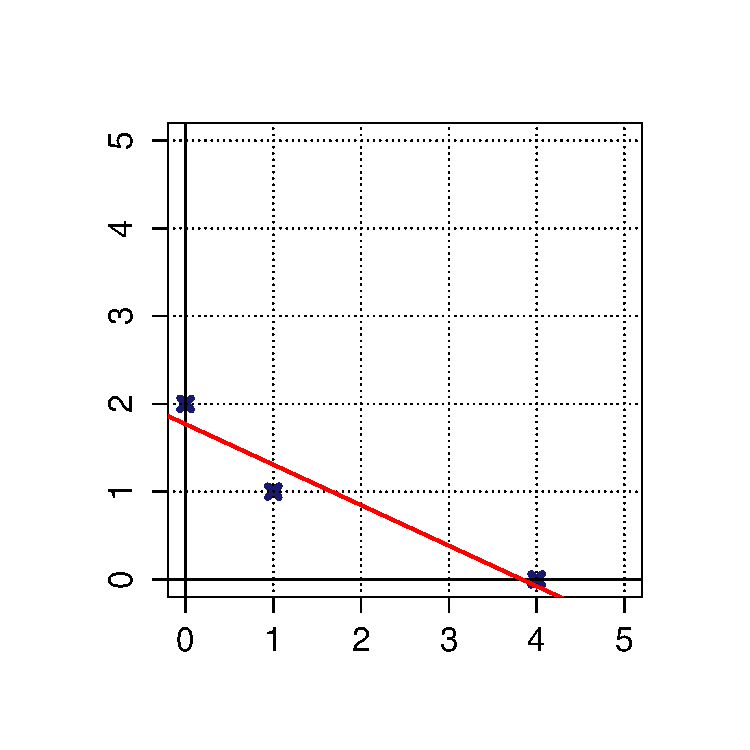
\includegraphics[scale=.5]{./Figures/F14.pdf}%
\figcaption{The best fit for the points (blue) line is in red.}
\end{minipage}
}


\subsection{Quadratic Forms and Principal Axes}

The final application of the material in this chapter is finding the principal axes of ellipses. We will see that this subject is the heart of principal components analysis and will hopefully then be a nice transition into our next chapter on precisely this analysis.

\subsubsection{Ellipses as Quadratic Forms}

A quadratic form is a function $Q:\mathbb{R}^n \rightarrow \mathbb{R}$ defined by
$$
Q({\bf x})=Q((x_1,\ldots,x_n))=\sum_{i=1}^{n} \sum_{j \leq i}a_{i,j} x_ix_j
$$
for any ${\bf x}=(x_1,\ldots,x_n)^T\in\mathbb{R}^n$. It is a polynomial $Q((x_1,\ldots,x_n))$ in the variables $x_1,\ldots,x_n$ that is homogeneous of degree $2$ such that
$$
Q(t{\bf x})=t^2Q({\bf x})
$$
for some scalar $t \in \mathbb{R}$. This means that the degrees of each of its constituent monomials is two. 

\ex{10}{
The quadratic form $S:\mathbb{R}^2\rightarrow\mathbb{R}$ defined by 
$$
S({\bf x})=S((x,y))=(x+y)^2=x^2+2xy+y^2
$$
defines a prototypical quadratic form.

Notice that generally
$$
(x_1+\cdots+x_n)^2=\sum_{i=1}^{n}x_i^2+2\sum_{i=1}^{n}\sum_{j<i}x_ix_j=\sum_{i=1}^{n}\sum_{j \leq i}(2-\delta_{i,j})x_ix_j
$$
where $\delta_{i,j}$ is Kronecker's Delta. Thus if $P:\mathbb{R}^n\rightarrow\mathbb{R}$ is a function defined by 
$$
P({\bf x})=P((x_1+\cdots+x_n))=(x_1+\cdots+x_n)^2
$$ 
then $P$ is a quadratic form where $a_{i,j}=2-\delta_{i,j}$. 
}

An equivalent way to define a quadratic form $Q:\mathbb{R}^n\rightarrow \mathbb{R}$ is
$$
Q({\bf x})=Q((x_1,\ldots,x_n))=\sum_{i=1}^{n} \sum_{j =1}^{n}c_{i,j} x_ix_j
$$
where transforming our first definition we have that
$$
c_{i,j}=
\begin{cases}
a_{i,j}&i=j\\
\frac{1}{2}a_{i,j}\text{ or }\frac{1}{2}a_{j,i}&i\neq j.
\end{cases}
$$

We halve the $a_{i,j}$ when $i \neq j$ because this second form counts both $x_ix_j$ and $x_jx_i$ in comparison to our first definition which counts only one of these. 

Consider a matrix $C$ such that $C_{i,j}=c_{i,j}$ then for ${\bf x}=(x_1,\ldots,x_n)^T \in \mathbb{R}^n$ 
$$
C{\bf x}=
\begin{bmatrix}
c_{1,1}x_1+&\cdots&+c_{1,n}x_n\\
\vdots&&\vdots\\
c_{n,1}x_1+&\cdots&+c_{n,n}x_n
\end{bmatrix}
=
\begin{bmatrix}
\sum_{j=1}^{n}c_{1,j}x_j\\
\vdots\\
\sum_{j=1}^{n}c_{n,j}x_j
\end{bmatrix}
$$
and so 
$$
\begin{aligned}
{\bf x}^TC{\bf x}&=(x_1,\ldots,x_n)
\begin{bmatrix}
\sum_{j=1}^{n}c_{1,j}x_j\\
\vdots\\
\sum_{j=1}^{n}c_{n,j}x_j
\end{bmatrix}\\
&=x_1\sum_{j=1}^{n}c_{1,j}x_j+\cdots+x_n\sum_{j=1}^{n}c_{n,j}x_j\\
&=\sum_{j=1}^{n}x_1c_{1,j}x_j+\cdots+\sum_{j=1}^{n}x_nc_{n,j}x_j\\
&=\sum_{i=1}^{n}\sum_{j=1}^{n}c_{i,j}x_ix_i=Q({\bf x}).
\end{aligned}
$$

Thus if $C$ is a matrix of coefficients as defined above then any quadratic form $Q$ may be defined as $Q({\bf x})={\bf x}^TC{\bf x}$. Furthermore since $C_{i,j}=c_{i,j}=c_{j,i}=C_{j,i}$ then $C$ is symmetric. Hence any quadratic form may be represented as
$$
Q({\bf x})={\bf x}^TC{\bf x}
$$ 
where $C$ is a symmetric matrix. 

\ex{11}{
Using the quadratic form $P$ from Example $10$, 
$$
P({\bf x})={\bf x}^T{\bf 1}{\bf 1}^T{\bf x}=
{\bf x}^T\begin{bmatrix}
1& \cdots& 1\\
\vdots& \ddots& \vdots\\
1& \cdots& 1
\end{bmatrix}{\bf x}
\text{ for }{\bf x}\in\mathbb{R}^n
$$
where ${\bf 1}=(1,\ldots,1)^T\in\mathbb{R}^n$ is a vector of $1's$.
}

For any quadratic form $Q$ defined by 
$$
Q({\bf x})={\bf x}^TA{\bf x}\text{ for }{\bf x}\in\mathbb{R}^n
$$
and some $n \times n$ symmetric matrix $A$ then the locus of points defined, for some scalar $c$, by
$$
Q({\bf x})=c^2
$$
is either an ellipsoid or hyperboloid. These are the $n$-dimensional generalizations of hyperbolas and ellipses. For convenience we assume that $c>0$ such that $c=\sqrt{c^2}$.

\ex{12}{

Consider the quadratic form $R:\mathbb{R}^2\rightarrow\mathbb{R}$ defined for ${\bf x}=(x,y)^T\in\mathbb{R}^2$ by 
$$
R({\bf x})=R((x,y))=\frac{1}{4}x^2+y^2.
$$
We plot $R({\bf x})=\frac{1}{4}x^2+y^2=1$ below in Figure 1.4.

\begin{minipage}{.8\linewidth}
\centering%
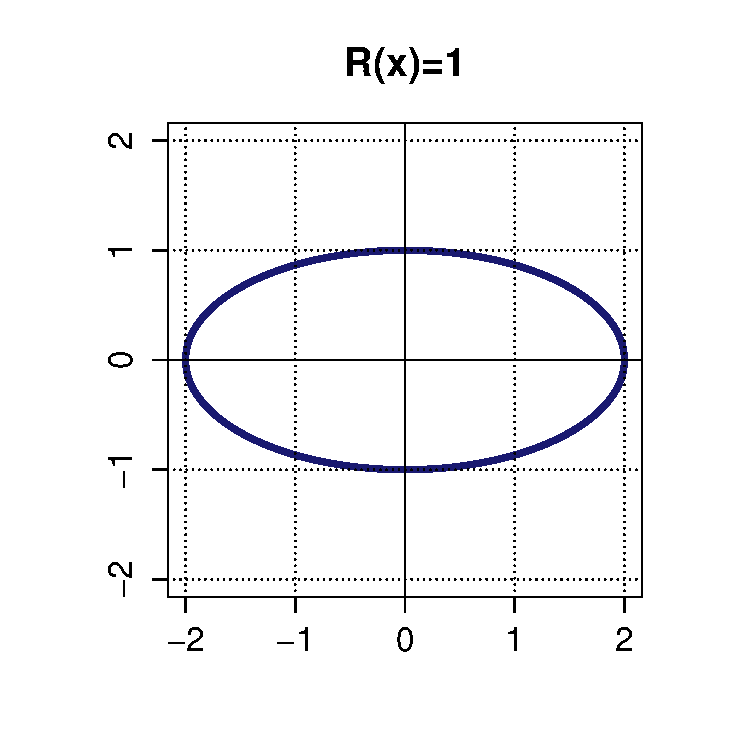
\includegraphics[scale=.5]{./Figures/F15.pdf}%
\figcaption{The quadratic form $R({\bf x})$ defines an ellipse in $\mathbb{R}^2$.}
\end{minipage}

}

\subsubsection{Principal Axes of Ellipsoids}

For our purposes we are interested in finding the principal axes of ellipsoids. We define the principal axes of an ellipsoid to be its axes of symmetry. We will see that this definition will need some clarification later but for now it will suffice. 

The principal axes of the quadratic form in Example 12 are easy to see. They are simply the $x$ and $y$ axes themselves. This is true because there are no mixed $xy$ terms in the defining polynoimal,
$$
R((x,y))=\frac{1}{4}x^2+0xy+y^2.
$$
This will generally be true. Consider a quadratic form $Q:\mathbb{R}^n\rightarrow\mathbb{R}$ and define an ellipsoid as the locus of points ${\bf x}\in\mathbb{R}^n$ where
$$
Q({\bf x})={\bf x}^TC{\bf x}=\sum_{i=1}^{n} \sum_{j =1}^{n}c_{i,j} x_ix_j=a^2
$$
for some constant $a>0$ and symmetric matrix $C$ where $C_{i,j}=c_{i,j}$. If there are no mixed terms $x_ix_j$ where $i \neq j$, i.e. $c_{i,j}=0$ when $i \neq j$, in the defining formula for $Q$ then the principal axes of the ellipsoid $Q({\bf x})=a^2$ align with the axes of the space. 


\thrm{10}{

{\bf The principal axes of a quadratic form $Q$ align with the space's axes if and only if there are no mixed terms in the defining polynomial.}\vspace{.5cm} 

 \emph{Proof.} \newline
$\Rightarrow$ To see this notice that if the principal axes align with the space axes then definitionally if we reflect any point ${\bf y}$ on the ellipsoid over any of the axes we should end up back on the ellipsoid. If this were not true then the ellipse  wouldn't have symmetry over the space's axes. Thus if ${\bf y}=(y_1,\ldots,y_k,\ldots,y_n)^T\in \mathbb{R}^n$ with $1\leq k\leq n$ is a point on the ellipsoid (i.e. $Q({\bf y})=a^2$) then define the point $\hat{\bf y}$ to be 
$$
\hat{\bf y}=(\hat{y}_1,\ldots,\hat{y}_n)^T=(y_1,\ldots,-y_k,\ldots,y_n)^T\in \mathbb{R}^n.
$$
This point better be on the ellipsoid because it is the reflection of ${\bf y}$ over one of the axes. Thus $Q(\hat{\bf y})=a^2$ and so
$$
Q({\bf y})=Q(\hat{\bf y})
$$
and hence
$$
\sum_{i=1}^{n} \sum_{j =1}^{n}c_{i,j} y_iy_j=\sum_{i=1}^{n} \sum_{j =1}^{n}c_{i,j} \hat{y}_i\hat{y}_j.
$$
for any ${\bf y}$ on the ellipsoid. Now surely the constant $a$ does not change the principal axes of the quadratic form. It only changes the length of the axes. Thus let us choose a constant $b$ so to make finding the principal axes nice. Consider some ${\bf x}\in\mathbb{R}^n$ such that the only non-zero elements of ${\bf x}$ are $x_k$ and $x_s$ for $s \neq k$ meaning
$$
{\bf x}=(0,\ldots,0,x_s,0,\ldots,0,x_k,0,\ldots,0)
$$
and 
$$
\hat{\bf x}=(0,\ldots,0,x_s,0,\ldots,0,-x_k,0,\ldots,0).
$$
and so if $Q({\bf x})=b^2$ for some scalar $b>0$ then $Q(\hat{\bf x})=b^2$. Thus 
$$
\begin{aligned}
Q({\bf x})&=\sum_{i=1}^{n} \sum_{j =1}^{n}c_{i,j} x_ix_j\\
&=c_{s,s} x_s^2+c_{s,k}x_sx_k+c_{k,s}x_kx_s+c_{k,k}x_k^2\\
&=c_{s,s} x_s^2+2c_{s,k}x_sx_k+c_{k,k}x_k^2
\end{aligned}
$$
and
$$
\begin{aligned}
Q(\hat{\bf x})&=\sum_{i=1}^{n} \sum_{j =1}^{n}c_{i,j} \hat{x}_i\hat{x}_j\\
&=c_{s,s}\hat{x}_s^2+c_{s,k}\hat{x}_s\hat{x}_k+c_{k,s}\hat{x}_k\hat{x}_s+c_{k,k}\hat{x}_k^2\\
&=c_{s,s}x_s^2-c_{s,k}x_sx_k-c_{k,s}x_kx_s+c_{k,k}x_k^2\\
&=c_{s,s}x_s^2-2c_{s,k}x_sx_k+c_{k,k}x_k^2
\end{aligned}
$$
and so since $Q({\bf x})=Q(\hat{\bf x})$ then 
$$
c_{s,s} x_s^2+2c_{s,k}x_sx_k+c_{k,k}x_k^2=c_{s,s}x_s^2-2c_{s,k}x_sx_k+c_{k,k}x_k^2
$$
or
$$
4c_{s,k}x_kx_s=0.
$$
It follows that since $x_k$ and $x_s$ are nonzero then $c_{s,k}=0$. Since we can do this for any $s$ and $k$ where $s\neq k$ then
$$
c_{i,j}=0\text{ for }i \neq j.
$$
This means that $C=diag((c_{i,i}))$ because the off diagonal elements are zero. Thus if the principal axes are the space's axes then there are no mixed terms. 

$\Leftarrow$ Notice that this argument can be run backwards. Clearly if there are no mixed terms then
$$
Q({\bf x})=c_{1,1}x_1^2+\cdots+c_{n,n}x_n^2
$$
and
$$
Q(\hat{\bf x})=Q({\bf x})
$$
and so the quadratic form has symmetry over the space axes. Thus the principal axes are the axes of the space
}

So we have determined the principal axes for quadratic forms determined by diagonal matrices (they are simply the axes of the space). Now to determine the principal axes for other ellipses we will operate as is the theme of this chapter and leverage the fact that symmetric matrices are orthogonally diagonalizable.

Consider an arbitrary quadratic form $P:\mathbb{R}^n\rightarrow\mathbb{R}$ defined by 
$$
P({\bf x})={\bf x}^TA{\bf x}\text{ for }{\bf x}\in\mathbb{R}^n
$$
and some symmetric $A$. Then $A$ is diagonalizable by an orthogonal similarity transformation
$$
D=U^TAU
$$
where $U$ is an orthogonal matrix whose columns are eigenvectors of $A$ and $D=diag(\lambda_1,\ldots,\lambda_n)$ is a diagonal matrix with the eigenvalues of $A$ on its diagonal. Let us make a change of basis (change of variable)
$$
{\bf y}=U^T{\bf x}
$$
such that ${\bf y}$ is the representation of ${\bf x}$ in the eigenbasis of $A$ defined by the columns of $U$. Then 
$$
{\bf x}=U{\bf y}
$$
and so 
$$
{\bf x}^TA{\bf x}=(U{\bf y})^TA(U{\bf y})={\bf y}^TU^TAU{\bf y}={\bf y}^TD{\bf y}.
$$

So since $D$ is a diagonal matrix defining the quadratic form under the $U$ basis then the principal axes of the ellipsoid $P({\bf y})=c^2$ under this basis are the axes of the space. However the axes of this space are not the standard basis axes they are the axes defined by the eigenbasis of $A$. Thus the principal axes are those axes defined by the orthonormal eigenvectors of $A$. 

Furthermore under the eigenbasis $U$ then
$$
P({\bf y})={\bf y}^TD{\bf y}=\lambda_1y_1^2+\cdots+\lambda_ny_n^2.
$$

Now a quadratic form can define an ellipse if and only if the eigenvalues of its defining matrix are all non-negative. We call matrices with non-negative eigenvalues positive semi-definite.

\thrm{11}{

{\bf A quadratic form $Q$ defined by $Q({\bf x})={\bf x}^TA{\bf x}$ for some $n \times n$ symmetric matrix $A$ and ${\bf x}\in\mathbb{R}^n$ defines an ellipsoid $Q({\bf x})=c^2$ for ${\bf x}\in\mathbb{R}^n$ and $c>0$ if and only if the eigenvalues of $A$ are non-negative.}\vspace{.5cm}

From the previous discussion we know that there is some basis under which the quadratic form $Q$ is defined by a diagonal matrix $D=diag(\lambda_1,\ldots,\lambda_n)$ where the $\lambda_i$ are the eigenvalues of $A$ and so there is some basis where
$$
Q({\bf x})={\bf x}^TD{\bf x}=\lambda_1x_1^2+\cdots+\lambda_nx_n^2.
$$

The equation $Q({\bf x})=c^2$ will define an ellipsoid if and only if the $\lambda_i$ are non-negative which is true if and only if the eigenvalues of $A$ are non-negative.
}

Notice that for a quadratic form $Q$ we have $Q({\bf x})\geq 0$ for all ${\bf x}\in\mathbb{R}^n$ if and only if the matrix defining $Q$ is positive semi-definite. Surely if all of the eigenvalues $\lambda_i$ are non-negative then, looking at our above formula, $Q({\bf x})\geq 0$ for all ${\bf x}\in\mathbb{R}^n$. Furthermore if there is some $k$ such that $\lambda_k$ that is negative then we can pick a ${\bf x}$ such that $Q({\bf x})<0$ by making the $x_k$ the only non-zero element of ${\bf x}$.

If f we call the $i^{th}$ principal axis the $i^{th}$ eigenvector of $A$ (ordered descending according to eigenvalues) then the length of the $i^{th}$ principal axis for $P({\bf x})=P({\bf y})=c^2$ is
$$
\frac{c}{\sqrt{\lambda_i}}.
$$
This follows because the length of the $i^{th}$ principal axis is simply the distance from the origin to the ellipse along the $i^{th}$ principal axis. It is simply the value $y_i$ such that
$$
P((0,\ldots,y_i,\ldots,0))=c^2.
$$
This means
$$
\lambda_iy_i^2=c^2
$$
or
$$
y_i=\frac{c}{\sqrt{\lambda_i}}.
$$
Notice that for ellipsoids $\lambda_i\geq 0$ and so $\frac{1}{\sqrt{\lambda_i}}$ is defined. 

\ex{13}{
Consider the matrix 
$$
A=\begin{bmatrix}
4& 8\\
11& 7\\
14& -2
\end{bmatrix}
$$
from Example $8$ and its associated symmetric form 
$$
A^TA=
\begin{bmatrix}
333& 81\\
81& 117
\end{bmatrix}
$$ 
Then we already determined the unit-eigenvectors of $A^TA$ to be the columns of the matrix
$$
V=
\frac{1}{27\sqrt{10}}\begin{bmatrix} 
81& -27\\
27& 81
\end{bmatrix}
$$
with associated eigenvalues of $\lambda_1=360$ and $\lambda_2=90$. Thus if $R:\mathbb{R}^2\rightarrow\mathbb{R}$ is a quadratic form defined by
$$
R({\bf x})={\bf x}^TA^TA{\bf x}\text{ for }{\bf x}\in\mathbb{R}^2
$$
and $E$ is the ellipse defined by $R({\bf x})=1$ for ${\bf x}\in\mathbb{R}^2$. Then the principal axes of this ellipse are determined by unit-eigenvectors and the lengths of these eigenvectors are 
$$
\frac{1}{6\sqrt{10}}\text{ and }\frac{1}{3\sqrt{10}}
$$
notice that these lengths are 
$$
\frac{1}{\sqrt{\lambda_i}}=\frac{1}{\sigma_i}
$$
where $\sigma_i$ is the $i^{th}$ singular value of $A$.

\newpage
\begin{minipage}{.8\linewidth}
\centering%
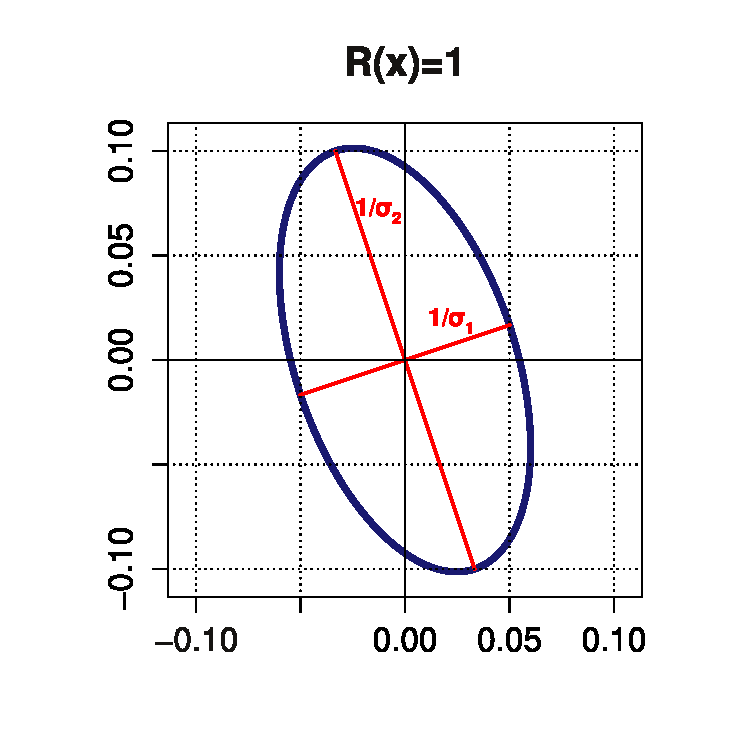
\includegraphics[scale=.5]{./Figures/F16.pdf}%
\figcaption{The quadratic form defined in Example 13. The lines are the axes of the ellipse.}
\end{minipage}

}

Although we defined \emph{the} principal axes to be the axes of symmetry there may be more than one set of axes for the space over which the ellipsoid is symmetric. The ellipse defined by
$$
{\bf x}^TI{\bf x}=1
$$
is one for which \emph{any} orthogonal basis of the space would define a set of principal axes. Thus as we saw with the singular value decomposition if there are repeated eigenvalues then there are infinite choices for the eigenvectors. The important point is that we can always find a new orthonormal basis for the space (a new set of axes) with respect to which the ellipse is symmetric. We call any such set a set of principal axes of the ellipse.















%%%%%%%%%%%%%%%%%%%%%%%%%%%%%%%%%%%%%%
\chapter{Multivariate Generalizations}

This chapter serves to introduce some of the multivariate generalization of statistical ideas of which we are familiar. As in Chapter 1 an understanding of this material greatly aids in understanding the later contributions of this paper. 

%This chapter serves to introduce principal components analysis. Principal components analysis (PCA) is widely popular multivariate method often used in exploratory data analysis.  With the information in Chapter 1 understood the development of PCA is not a very laborious ordeal. This chapter will introduce some of the statistical notions needed to understand PCA, introduce the method itself, and give examples of the method both in theory and through case studies.

\section{Covariance and Correlation}

The first order of business is to extend some of the familiar univariate statistical notions into a multivariate setting. Thus instead of considering for some sample space $\Omega$ a random scalar $\mathscr{X}:\Omega\rightarrow\mathbb{R}$ we consider a random vector $\bs{\mathscr{X}}:\Omega\rightarrow\mathbb{R}^p$ such that
$$
\bs{\mathscr{X}}=(\mathscr{X}_1,\cdots,\mathscr{X}_p)^T
$$
where $\{\mathscr{X}_i\}_{i=1}^{p}$ are random scalars. Similarly to random vectors we may consider a random matrix 
$$
Y:\Omega\rightarrow\mathbb{R}^{n\times p}\text{ where }Y_{i,j}=\mathscr{Y}_{i,j}
$$
for some set of random scalars $\{\mathscr{Y}_{i,j}\}_{i=1}^{n} \,_{j=1}^{p}$.

\subsection{The Covariance and Correlation Matrices}

One of the most important concepts in multivariate statistics is the variance-covariance matrix. Also known as the covariance or dispersion matrix it is the multivariate generalization of variance. As with the univariate variance we may define it both for the theoretical probability distribution of a population as well as an estimate obtained by sampling from the population. 

Consider a random vector $\bs{\mathscr{X}}=(\mathscr{X}_1,\ldots,\mathscr{X}_p)^T$ comprised of $p$ random scalars $\{\mathscr{X}_i\}_{i=1}^{p}$. We define the variance-covariance matrix $\text{var}\left[\rv{X}\right]=\Sigma$ to be the matrix such that
$$
\Sigma_{i,j}=\text{cov}[\mathscr{X}_i,\mathscr{X}_j].
$$
We can write this in another form as
$$
\Sigma=\text{E}[(\bs{\mathscr{X}}-\text{E}[\bs{\mathscr{X}}])(\bs{\mathscr{X}}-\text{E}[\bs{\mathscr{X}}])^T]
$$
where the expectation of a random matrix (or vector) is the element-wise expectation and, furthermore, multiplication of random matrices (or vectors) is defined in precise analogy to that of real matrices (or vectors). 

The equality of the two definitions may be seen because
$$
\Sigma_{i,j}=\e{(\rv{X}-\e{\rv{X}})_i(\rv{X}-\e{\rv{X}})_j}=\e{(\mathscr{X}_i-\e{\mathscr{X}_i})(\mathscr{X}_j-\e{\mathscr{X}_j})}=\cov{\mathscr{X}_i}{\mathscr{X}_j}.
$$
In either case the covariance of $\mathscr{X}_i$ and $\mathscr{X}_j$, denoted $\sigma_{x_i,x_j}$, is the $(i,j)^{th}$ entry of the covariance matrix $\Sigma$. 

Let us have taken $n$ observations of $\rv{X}$. This is tantamount to $n$ simultaneous observations of each of the $p$ random variables $\mathscr{X}_i$. We may similarly define an unbiased estimator of $\Sigma$ as the sample covariance matrix $S$ such that 
$$
S_{i,j}=s_{\mathscr{X}_i,\mathscr{X}_j}
$$
where $s_{\mathscr{X}_i,\mathscr{X}_j}$ is the univariate sample covariance between $\mathscr{X}_i$ and $\mathscr{X}_j$. Then leveraging the univariate definition for sample covariance we have that 
$$
S_{i,j}=\frac{1}{n-1}\sum_{k=1}^{n}(x_{k,i}-m_i)(x_{k,j}-m_j)
$$
where $x_{s,t}$ is the $s^{th}$ observation of $\mathscr{X}_t$ and $m_i=\frac{1}{n}\sum_{k=1}^{n}x_{k,i}$ is the arithmetic mean of the sample of $\mathscr{X}_i$ and similarly for $m_j$. 

This notation is very messy so let us simplify it with vector notation. Define ${\bf x_j}\in\mathbb{R}^n$ for $j=1,\ldots,p$ to be a vector containing the observations of $\mathscr{X}_j$. That is 
$$
{\bf x_j}=(x_{1,j},\ldots,x_{n,j})^T
$$
where $x_{i,j}$ is the $i^{th}$ observation of variable $\mathscr{X}_j$. Then if 
$$
{\bf m_j}=(m_j,\ldots,m_j)^T=m_j(\overset{n}{\overbrace{1,\ldots,1}})^T\in\mathbb{R}^n
$$ 
is the vector containing $m_j$ in all $n$ entries then
$$
S_{i,j}=\frac{1}{n-1}({\bf x_i}-{\bf m_i})^T({\bf x_j}-{\bf m_j}).
$$

Since $S_{i,j}$ is simply the univariate covariance among two random scalars $\mathscr{X}_i$ and $\mathscr{X}_j$ then the above gives a new way of writing the univariate covariance or indeed univariate variance. For a univariate random variable $\mathscr{Y}$ with observation vector ${\bf y}\in\mathbb{R}^n$ its univariate variance estimation may be written as
$$
s_\mathscr{Y}^2=\frac{1}{n-1}({\bf y}-{\overline {\bf y}})^T({\bf y}-{\overline {\bf y}})
$$
where $\overline{{\bf y}}=\frac{1}{n}\sum_{i=1}^{n}y_i$ is the mean vector for ${\bf y}$. This should look very familiar to our definition for the covariance matrix $\Sigma$. Remember that we said $\Sigma$ and $S$ are the generalization of univariate variance. Thus it should not be surprising that we can write the sample covariance matrix $S$ in a very analogous form. 

Define the data matrix $X$ as
$$
X=
\begin{bmatrix}
{\bf x_1}& \cdots& {\bf x_p}
\end{bmatrix}
$$
having as its $j^{th}$ column the vector ${\bf x_j}$. We call this the data matrix because the $(i,j)^{th}$ entry of $X$ is the $i^{th}$ observation of the random variable $\mathscr{X}_j$. Alternatively the $(i,j)^{th}$ entry is the $j^{th}$ variable $\mathscr{X}_j$ measured in the $i^{th}$ observation. Each \emph{row} of $X$ is one of the $n$ observations of $\rv{X}$. Alternatively we could define the data matrix in a row major manner such that 
$$
X=\begin{bmatrix}
\mathscr{O}_1\\
\vdots\\
\mathscr{O}_n\\
\end{bmatrix}
$$
where $\mathscr{O}_i$ for $i=1,\ldots,n$ is the $i^{th}$ observation of $\rv{X}=(\mathscr{X}_1,\ldots,\mathscr{X}_p)^T$. (Admittedly since $\rv{X}$ is a random \emph{column} vector it would have been better to define $X$ as having as each of its \emph{columns} one of the observations of $\rv{X}$ however this is not the usual convention. Thus we will not buck the trend and use the customary definition for a data matrix.)

Let us also define the mean matrix as follows. Let ${\bf 1}_p\in\mathbb{R}^p$ to be the vector of all 1's such that ${\bf 1}=(1,\ldots,1)\in\mathbb{R}^p$ and define $D=diag(m_1,m_2,\ldots,m_p)$ to an $p \times p$ diagonal matrix with $i^{th}$ diagonal entry as the arithmetic mean of the sample of $\mathscr{X}_i$. Then the matrix ${\bf 1}_n{\bf 1}_p^T$ is a $n \times p$ matrix of all 1's and so the matrix $M$ defined by 
$$
M={\bf 1}_n{\bf 1}_p^TD=
\begin{bmatrix}
1& \cdots& 1\\
\vdots& \ddots& \vdots\\
1& \cdots& 1\\
\end{bmatrix}
\begin{bmatrix}
m_p& & \\
& \ddots& \\
& & m_p
\end{bmatrix}
=
\begin{bmatrix}
m_1& \cdots& m_p\\
\vdots& \ddots& \vdots\\
m_1& \cdots& m_p
\end{bmatrix}
$$
is a matrix whose columns are the mean vectors ${\bf m_i}$.

Thus we have that
$$
X=
\begin{bmatrix}
{\bf x_1}& \cdots& {\bf x_p}
\end{bmatrix}
\text{ and }
M=\begin{bmatrix}
{\bf m_1}& \cdots& {\bf m_p}
\end{bmatrix}
$$
and so 
$$
X-M=
\begin{bmatrix}
{\bf x_1}-{\bf m_1}& \cdots& {\bf x_p}-{\bf m_p}
\end{bmatrix}.
$$
Note the similarity of
$$
\rv{X}=(\mathscr{X}_1,\ldots,\mathscr{X}_p)^T\text{ to }X=\begin{bmatrix}{\bf x_1}& \cdots& {\bf x_p}\end{bmatrix}
$$
and
$$
\e{\rv{X}}=(\e{\mathscr{X}_1},\ldots,\e{\mathscr{X}_p})^T\text{ to }M=\begin{bmatrix}{\bf m_1}& \cdots& {\bf m_p}\end{bmatrix}.
$$

Then analogously to the definition of the variance for the univariate random variable $\mathscr{Y}$ and similarly to how we defined $\Sigma$ we can define the sample covariance matrix $S$ of the data matrix $X$ as
$$
S=\frac{1}{n-1}(X-M)^T(X-M).
$$
We can see this because
$$
\begin{aligned}
\left(\frac{1}{n-1}(X-M)^T(X-M)\right)_{i,j}&=\frac{1}{n-1}row\left(i,(X-M)^T\right)col(j,X-M)\\
&=\frac{1}{n-1}col(i,X-M)^Tcol(j,X-M)
\end{aligned}
$$
which is precisely 
$$
\frac{1}{n-1}({\bf x_i}-{\bf m_i})^T({\bf x_j}-{\bf m_j})=s_{\mathscr{X}_i,\mathscr{X}_j}.
$$

As with the univariate case we can define correlation from a definition of covariance. Given the same random vector $\rv{X}=\left(\mathscr{X}_1,\ldots,\mathscr{X}_n\right)^T$ we can define the correlation matrix $P$ as 
$$
P_{i.j}=\rho_{\mathscr{X}_i,\mathscr{X}_j}=\frac{\sigma_{\mathscr{X}_i,\mathscr{X}_j}}{\sigma_{\mathscr{X}_i}\sigma_{\mathscr{X}_j}}
$$
so that the $(i,j)^{th}$ entry of $P$ is the correlation between $\mathscr{X}_i$ and $\mathscr{X}_j$.

Similarly if we have made $n$ observations then we can define a sample correlation matrix $R$ as
$$
R_{i,j}=r_{\mathscr{X}_i,\mathscr{X}_j}=\frac{s_{\mathscr{X}_i,\mathscr{X}_j}}{s_{\mathscr{X}_i}s_{\mathscr{X}_j}}.
$$

If we take our data matrix $X$ from previously and define a scaling matrix $A$ such that $A=diag(1/s_{\mathscr{X}_1},\ldots,1/s_{\mathscr{X}_p})$ then right multiplication by $A$ gives us
$$
(X-M)A=
\begin{bmatrix}
({\bf x_1}-{\bf m_1})/s_{\mathscr{X}_1}& \cdots& ({\bf x_p}-{\bf m_p})/s_{\mathscr{X}_p}
\end{bmatrix}.
$$
which standardizes the columns of $X-M$ and so
$$
R=\frac{1}{n-1}((X-M)A)^T(X-M)A=\frac{1}{n-1}A(X-M)^T(X-M)A.
$$
This is easy to see since $S=\frac{1}{n-1}(X-M)^T(X-M)$ is our covariance matrix and multiplying by $A$ on the right scales the $j^{th}$ column of $S$ by $1/s_{\mathscr{X}_j}$ and multiplying by $A$ on the left scales the $i^{th}$ row by $1/s_{\mathscr{X}_i}$ giving us that
$$
\left(A\left(\frac{1}{n-1}(X-M)^T(X-M)\right)A\right)_{i,j}=\frac{S_{i,j}}{s_{\mathscr{X}_i}s_{\mathscr{X}_j}}=\frac{s_{\mathscr{X}_i,\mathscr{X}_j}}{s_{\mathscr{X}_i}s_{\mathscr{X}_j}}=r_{\mathscr{X}_i,\mathscr{X}_j}.
$$

Note that a nearly identical argument can be made in forming the correlation matrix $P$ by scaling component random scalars $\mathscr{X}_i$ of $\rv{X}$ by their respective variances and finding the covariance matrix of the standardized random vector $B\rv{X}$ where $B=diag(1/\sigma_1,\ldots,1/\sigma_p)$.

\newpage
\ex{1}{
Consider the $5 \times 3$ data matrix $X$ of $5$ measurements of $3$ variables 
$$
X=
\begin{bmatrix}
4.0& 2.0& .6\\
4.2& 2.1& .59\\
3.9& 2.0& .58\\
4.3& 2.1& .62\\
4.1& 2.2& .63
\end{bmatrix}.
$$
Then the means of the columns are $(4.1,2.08,.604)$ and so the mean matrix is
$$
M=\begin{bmatrix}
4.1& 2.08& .604\\
4.1& 2.08& .604\\
4.1& 2.08& .604\\
4.1& 2.08& .604\\
4.1& 2.08& .604\\
\end{bmatrix}
\text{ meaning }
X-M=
\begin{bmatrix}
-.1& -.08& -.004\\
.1& .02& -.014\\
-.2& -.08& -.024\\
.2& .02& .016\\
0&  .12&  .026
\end{bmatrix}
$$

Then the sample covariance matrix is 
$$
S=\frac{1}{5-1}(X-M)^T(X-M)=
\begin{bmatrix}
.025& .0075& .00175\\
.0075& .007& .00135\\
.00175& .00135& .0043
\end{bmatrix}.
$$

The diagonals of this matrix are the variances and so their square roots are the standard deviations meaning
$$
s_1=.1581,s_2=.0836\text{ and }s_3=.0207
$$
and so if $A=diag(1/s_1,1/s_2,1/s_3)$ then $(X-M)A$ standardizes the columns of $X-M$ and so 
$$
(X-M)A=
\begin{bmatrix}
-.6324& -.9561& -.1928\\
.0632& .2390& -.6751\\
-1.264& -.9561& -1.157\\
1.264& .2390& .7715\\
0& 1.434& 1.253
\end{bmatrix}
$$
meaning the sample correlation matrix $R$ is
$$
R=\frac{1}{4}A(X-M)^T(X-M)A=
\begin{bmatrix}
1& .5669& .5337\\
.5669& 1& .7781\\
.5337& .7781& 1
\end{bmatrix}.
$$
}

\subsection{Properties and Linear Combinations}

The manner in which we defined the sample correlation matrix (via right multiplication by a matrix $A$) can be generalized into an important fact that will be our first theorem of this chapter. Consider an $n \times p$ data matrix $X$ and a $p \times m$ real matrix $L$. Then let $Y$ be the product $XL$ such that 
$$
\begin{aligned}
Y=XL&=
\begin{bmatrix}
{\bf x_1}& \cdots& {\bf x_p}
\end{bmatrix}
\begin{bmatrix}
{\bf L_1}& \cdots& {\bf L_m}
\end{bmatrix}\\
&=
\begin{bmatrix}
L_{1,1}{\bf x_1}+\cdots+L_{p,1}{\bf x_p}& \cdots& L_{1,m}{\bf x_1}+\cdots+L_{p,m}{\bf x_p}
\end{bmatrix}
\end{aligned}
$$
such that each column of $Y=XL$ is a linear combination of the observation vectors $\{{\bf x_i}\}_{i=1}^{p}$. That is,
$$
col(j,Y)=col(j,XL)=L_{1,j}{\bf x_1}+\cdots+L_{p,j}{\bf x_p}
$$
and so whereas the $j^{th}$ column of $X$ represented the observation vector of $\mathscr{X}_j$ the $j^{th}$ column of $XL$ represents the observation vector of a new random scalar
$$
\mathscr{Y}_j=L_{1,j}\mathscr{X}_1+\cdots+L_{p,j}\mathscr{X}_p.
$$
Thus while the matrix $X$ is a data matrix for samples of the random vector $\rv{X}:\Omega\rightarrow\mathbb{R}^p$ the matrix $Y=XL$ is a data matrix for samples of the random vector $\rv{Y}=L^T\rv{X}$ which maps $\Omega\mapsto\mathbb{R}^m$ where
$$
\begin{aligned}
\rv{Y}=L^T\rv{X}&=\begin{bmatrix}\overset{\text{------}}{\hfill}{\bf L_1}\overset{\text{------}}{\hfill}\\  \vdots \\  \overset{\text{------}}{\hfill}{\bf L_m} \overset{\text{------}}{\hfill}\end{bmatrix}\begin{bmatrix}\mathscr{X}_1\\\vdots\\\mathscr{X}_p\end{bmatrix}\\
&=(L_{1,1}\mathscr{X}_1+\cdots+L_{p,1}\mathscr{X}_p,\,\ldots,\, L_{1,m}\mathscr{X}_1+\cdots+L_{p,m}\mathscr{X}_p)\\
&=(\mathscr{Y}_1,\ldots,\mathscr{Y}_m).
\end{aligned}
$$
Let us prove an important theorem about such linear combinations.


\thrm{1}{

{\bf Consider a random vector $\rv{X}$ with associated covariance matrix $\Sigma$ and $n \times p$ sample data matrix $X$ with sample covariance matrix $S$. If $L$ is a $p \times m$ matrix then the covariance matrix of the random vector $L^T\rv{X}$ is $L^T\Sigma L$ and the sample covariance matrix associated with the data matrix $XL$ of $L^T\rv{X}$ is $L^TSL$.}\vspace{.5cm}

We already established that the data matrix for $L^T\rv{X}$ is $XL$ and it is easy to show that if the sample mean matrix of $\rv{X}$ is $M$ then the sample mean matrix of $L^T\rv{X}$ is $ML$ since average plays nicely with linear operators such as matrix multiplication. Thus the sample covariance matrix of $L^T\rv{X}$ is 
$$
\begin{aligned}
S_{L}&=\frac{1}{n-1}(XL-ML)^T(XL-ML)\\
&=\frac{1}{n-1}L^T(X-M)^T(X-M)L\\
&=L^T\left(\frac{1}{n-1}(X-M)^T(X-M)\right)L\\
&=L^TSL.
\end{aligned}
$$

This is also true for the covariance matrix $\Sigma$ of $\rv{X}$ because of its analogous definition. The covariance matrix of $L^T\rv{X}$ is 
$$
\begin{aligned}
\Sigma_L&=\e{(L^T\rv{X}-\e{L^T\rv{X}})(L^T\rv{X}-\e{L^T\rv{X}})^T}\\
&=\e{(L^T\rv{X}-L^T\e{\rv{X}})(L^T\rv{X}-L^T\e{\rv{X}})^T}\\
&=\e{(L^T(\rv{X}-\e{\rv{X}}))(L^T(\rv{X}-\e{\rv{X}}))^T}\\
&=\e{L^T(\rv{X}-\e{\rv{X}})(\rv{X}-\e{\rv{X}})^TL}\\
&=L^T\e{(\rv{X}-\e{\rv{X}})(\rv{X}-\e{\rv{X}})^T}L\\
&=L^T\Sigma L.
\end{aligned}
$$
}

Consider a random vector $\rv{X}:\Omega\rightarrow\mathbb{R}^p$ with covariance matrix $\Sigma$. If we let $B$ be the $p \times p$ diagonal matrix $B=diag(1/\sigma_1,\ldots,1/\sigma_p)$ then the covariance matrix of $B\rv{X}$ is
$$
\Sigma_B=B\Sigma B
$$
which is precisely the correlation matrix $P$. Similarly if we have a $p \times p$ sample covariance matrix $S$ of $\rv{X}$ and $A=diag(1/s_1,\ldots,1/s_p)$ then the sample covariance matrix of $A\rv{X}$ is
$$
S_A=ASA
$$ 
which is the sample correlation matrix $R$. 

Thus in general the correlation matrix $P$ is simply the covariance matrix of the standardized random vector $\rv{Y}=\left(\frac{\mathscr{X}_1}{\sigma_1},\ldots,\frac{\mathscr{X}_p}{\sigma_p}\right)^T$. Similarly the sample correlation matrix $R$ is the sample covariance matrix of the associated standardized data matrix with columns $Y=\left[\frac{{\bf x_1}}{s_1}\,\cdots\,\frac{{\bf x_1}}{s_1}\right]$. Thus all correlation matrices are covariance matrices. If not stated otherwise we may now assume that all results on the covariance matrix extends to the correlation matrix.

Our definitions of the covariance and sample covariance matrices $\Sigma$ and $S$ hint at another property. We define these matrices multiplying a suitable matrix (or vector) by its transpose. Consider the sample covariance and correlation matrices $S$ and $R$. These (and also $\Sigma$ and $P$) are symmetric. We can see this because in the case of $S$,
$$
S_{i,j}=s_{\mathscr{X}_i,\mathscr{X}_j}=s_{\mathscr{X}_j,\mathscr{X}_i}=S_{j,i}.
$$
and similarly for $R$ (and $\Sigma$ or $P$). More richly however notice that for $B=\frac{1}{\sqrt{n-1}}(X-M)$ 
$$
S=B^TB
$$
which is a symmetric form that should bring to mind much of the last chapter. A similar story may be told for $R$ since for $C=\frac{1}{\sqrt{n-1}}(X-M)A$ we have $R=C^TC$ and, recalling the definitions for $\Sigma$ and $P$, it is true for these matrices also. However we know much more from last chapter about these forms than that they are simply symmetric. The next theorem will be the first of many applications of last chapter's material given what we now know about these matrices.

\thrm{2}{
{\bf A matrix $M$ is a covariance matrix if and only if it positive semi-definite.}\vspace{.5cm}

$\Rightarrow$ We already showed in the previous chapter that the symmetric form $A^TA$ has non-negative eigenvalues for a real $A$ and so since the sample covariance matrix is
$$
S=\left(\frac{1}{\sqrt{n-1}}X\right)^T\left(\frac{1}{\sqrt{n-1}}X\right)
$$
where $\frac{1}{\sqrt{n-1}}X$ is real then $S$ has non-negative eigenvalues and is thus positive semi-definite. 

On the other hand for a random variable $\rv{X}=(\mathscr{X}_1,\ldots,\mathscr{X}_p)^T$ with covariance matrix $\Sigma$ and $p \times 1$ vector 
$$
L=(l_1,\ldots,l_p)^T
$$ 
then the variance of the univariate random variable defined by the linear combination 
$$
l_1\mathscr{X}_1+\cdots+l_p\mathscr{X}_p
$$ 
is the ($1 \times 1$) covariance matrix of $L^T\rv{X}$. Theorem 1 tells us that this is
$$
\Sigma_{L^T\rv{X}}=L^T\Sigma L.
$$
Since this is the covariance of a univariate random variable then $L^T\Sigma L\geq 0$ however $L^T\Sigma L$ is a quadratic form in $L$. Thus, as we discovered in the previous chapter, $\Sigma$ must be positive semi-definite since its associated quadratic form is non-negative.

$\Leftarrow$ Now for the reverse direction consider a symmetric positive semi-definite $M$. Then $M$ is orthogonally diagonalizable as
$$
M=UDU^T
$$
for some orthogonal matrix $U$ and diagonal matrix $D$. Then define the square root of $M$ to be
$$
\sqrt{M}=U\sqrt{D}U^T
$$
where if $D=diag(\lambda_1,\ldots,\lambda_p)$ then $\sqrt{D}=diag(\sqrt{\lambda_1},\ldots,\sqrt{\lambda_p})$. This okay because $M$ is positive semi-definite and so its eigenvalues are non-negative since so a real square root exists for $\lambda_i$. With this definition then
$$
\left(\sqrt{M}\right)^2=U\sqrt{M}U^TU\sqrt{M}U^T=U\left(\sqrt{D}\right)^2U^T=UDU^T=M
$$
and
$$
\left(\sqrt{M}\right)^T=(U\sqrt{D}U^T)^T=(U^T)^T\left(\sqrt{D}\right)U^T=U\sqrt{D}U^T=\sqrt{M}.
$$

Now if $\rv{X}$ is a random vector with identity covariance structure ($\Sigma=I$) then we know from Theorem 1 that
$$
\text{var}\left[\sqrt{M}\rv{X}\right]=\left(\sqrt{M}\right)^T\text{var}[\rv{X}]\sqrt{M}=\sqrt{M}I\sqrt{M}=\left(\sqrt{M}\right)^2=M.
$$
Thus $M$ is the covariance matrix of $\sqrt{M}\rv{X}$ and so it is the covariance matrix of some random vector. A similar result is available for the sample covariance matrix $S$.
}

Since all correlation matrices are also covariance matrices then the above theorem is true for them also. 

\subsection{The Frobenius Norm}

In the spirit of generalizing we would like to define a norm for matrices. Normally we deal with norms of vectors. The norm of a vector
$$
{\bf x}=(x_1,\ldots,x_p)^T\in\mathbb{R}^p
$$ 
is defined as 
$$
||{\bf x}||=\sqrt{\sum_{i=1}^{p}x_i^2}=\sqrt{{\bf x}^T{\bf x}}.
$$
For a real $n \times p$ matrix $A$ we may define a norm, called the Frobenius norm, as 
$$
||A||_F=\sqrt{\sum_{j=1}^{p}\sum_{i=1}^{n}A_{i,j}^2}=\sqrt{tr(A^TA)}=\sqrt{tr(AA^T)}
$$
where $tr(B)$ is the trace of a square $p \times p$ matrix $B$ defined by $tr(B)=\sum_{i=1}^{p}B_{i,i}$ the sum of its diagonal elements. Notice how analogously we define the matrix norm. Just as with a vector it is the square root of the sum of the constituent components. Indeed when $A$ is a vector ($1 \times p$ or $p \times 1$ matrix) then the Frobenius norm reduces to the familiar Euclidean norm for vectors. 

We can see that $\sqrt{\sum_{j=1}^{p}\sum_{i=1}^{n}A_{i,j}^2}=\sqrt{tr(A^TA)}$ because
$$
(A^TA)_{i,j}=row(i,A^T)col(j,A)=col(i,A)^Tcol(j,A)
$$
and so 
$$
(A^TA)_{j,j}=col(j,A)^Tcol(j,A)=||col(j,A)||^2=\sum_{i=1}^{n}A_{i,j}^2.
$$
This means that
$$
tr(A^TA)=\sum_{j=1}^{p}\sum_{i=1}^{n}A_{i,j}^2
$$
and so 
$$
\sqrt{tr(A^TA)}=\sqrt{\sum_{j=1}^{p}\sum_{i=1}^{n}A_{i,j}^2}.
$$

Now the trace of $A^TA$ is equal to the sum of the eigenvalues of $A^TA$. To see this note that $A^TA$ is a $p \times p$ square matrix and we proved last chapter that it had $p$ real eigenvalues. Furthermore since it is symmetric it is orthogonally diagonalizable as
$$
D=U^TA^TAU
$$
and so
$$
tr(D)=tr(U^TA^TAU)
$$
and so since $tr(YZ)=tr(ZY)$ for same sized matrices $Y$ and $Z$ then
$$
tr(D)=tr(U^TA^TAU)=tr(UU^TA^TA)=tr(A^TA).
$$
Thus since $D=diag(\lambda_1,\ldots,\lambda_p)$ is a diagonal with matrix of eigenvalues
$$
tr(A^TA)=tr(D)=\sum_{i=1}^{p}\lambda_i.
$$
Hence
$$
||A||_F=\sqrt{tr(A^TA)}=\sqrt{\sum_{i=1}^{p}\lambda_i}.
$$
We can play the same game with $AA^T$ and get that $||A||_F=\sqrt{tr(A^TA)}=\sqrt{tr(AA^T)}=\sqrt{\sum_{i=1}^{p}\lambda_i}$ since the non-zero eigenvalues of $A^TA$ and $AA^T$ are the same. However we defined the non-zero singular values of $A$ to be the square roots of the eigenvalues of $A^TA$ (or $AA^T$) and so $\lambda_i=\sigma_i^2$ meaning
$$
||A||_F=\sqrt{\sum_{i=1}^{s}\sigma_i^2}
$$
where $s\leq min\{n,p\}$ is the number of non-zero singular values. 

There is another important way we can see this. The trick of switching the order of the trace of a product can be used to show that the Frobenius norm is invariant under multiplication by orthogonal matrices. For some orthogonal matrix $U$
$$
||AU||_F=\sqrt{tr(U^TA^TAU)}=\sqrt{tr(UU^TA^TA)}=\sqrt{tr(A^TA)}=||A||_F
$$
and similarly
$$
||UA||_F=||A||_F.
$$
Thus if $A$ has a singular value decomposition $A=U\Sigma V^T$ for orthogonal $U$ and $V$ then
$$
||A||_F=||U\Sigma V^T||_F=||\Sigma||_F=\sqrt{tr(\Sigma^T\Sigma)}=\sqrt{\sum_{i=1}^{s}\sigma_i^2}.
$$

This fact should not be surprising as the we already know that for a matrix $A$ the singular values $\sigma_i$ tell us how much vectors in the row space are stretched when sent into the column space. As with vector norms matrix norms are trying to tell us something about the size of a matrix. Thus it seems sensible that the Frobenius norm tells us something about how much the matrix stretches the space (and the vectors in it).

\subsection{Total Variance}
We would like to define a summary statistic for the covariance matrix that can give us an overall picture. After all the covariance matrix has $\binom{p+1}{2}$ unique entries and so this is quite a lot of information to take in at once. Let us define the total variance of a random vector $\rv{X}=(\mathscr{X}_1,\ldots,\mathscr{X}_p)^T$ with associated covariance matrix $\Sigma$ to be
$$
\text{total variance}=tr(\Sigma)=\sum_{i=1}^{p}\sigma_{\mathscr{X}_i}^2.
$$
Notice that if we define the Frobenius norm of a random matrix $Y$ to be the square root of the trace of its symmetric form $YY^T$ then
$$
\begin{aligned}
||(\rv{X}-\e{\rv{X}})||_F^2&=tr\left((\rv{X}-\e{\rv{X}})(\rv{X}-\e{\rv{X}})^T\right)\\
&=\sum_{i=1}^{p}(\mathscr{X}_i-\e{\mathscr{X}_i})^2
\end{aligned}
$$
and so 
$$
\begin{aligned}
\e{||(\rv{X}-\e{\rv{X}})||_F^2}&=\e{\sum_{i=1}^{p}(\mathscr{X}_i-\e{\mathscr{X}_i})^2}\\
&=\sum_{i=1}^{p}\e{(\mathscr{X}_i-\e{\mathscr{X}_i})^2}\\
&=\sum_{i=1}^{p}\sigma_i^2.
\end{aligned}
$$
Thus the total variance of a random vector $\rv{X}$ is the expectation of the squared Frobenius norm of the centered random vector $\rv{X}-\e{\rv{X}}$.


Similarly if the associated sample covariance matrix of $n$ observations of $\rv{X}$ is $S$ then define
$$
\text{total sample variance}=tr(S)=\sum_{i=1}^{p}s_{\mathscr{X}_i}^2.
$$
Remember that if $X$ is the data matrix of the $n$ observations of $\rv{X}$ then
$$
S=\frac{1}{n-1}(X-M)^T(X-M)
$$ 
for associated mean matrix $M$ and so
$$
tr(S)=tr\left(\frac{1}{n-1}(X-M)^T(X-M)\right)
$$ 
or if $Y=\frac{1}{\sqrt{N-1}}(X-M)$ then
$$
tr(S)=tr\left(Y^TY\right)=||Y||^2_F=\frac{1}{n-1}||X-M||^2_F.
$$
Thus the total variance is proportional to the squared Frobenius norm of the centered data matrix $X-M$. Notice that this implies that the total variance is proportional to the sum of the squares of the singular values of $X-M$. Put another way, it is proportional to the sum of the eigenvalues of the sample covariance matrix.


\ex{2}{

Considering the sample covariance matrix from Example 1 let us compute the total sample variance. One definition is that
$$
\text{ total sample variance }=tr(S)=.03243\approx.025+.007+.0043
$$
or taking the Frobenius norm of $X$ we see that
$$
||X-M||_F=.3601
$$
and so
$$
\frac{1}{4}||X-M||_F^2=.03243.
$$
}

Note that the total variance is only one way to define a summary statistic for the covariance matrix. We introduce this notion in particular because it is the most natural such statistic when doing principal components analysis.


\section{The Normal Distribution}

The last generalization we want to make is that of the normal distribution. In the first part of this section we will develop a couple important features of the univariate normal distribution. While the univariate normal distribution is likely quite familiar developing its properties will be helpful in seeing the development of analogous properties in the more general  multivariate normal distribution. 

\subsection{The Univariate Case}

A univariate normally distributed random variable $\mathscr{X}$ is a simple model of a phenomena in which samples tend to be clustered around some center. The distribution is parameterized by two parameters $\mu=\e{\mathscr{X}}$ and $\sigma^2=\text{var}\left[\mathscr{X}\right]$. The goal of this first section is to show how these parameters control for location and spread of the data respectively. 

For a positive spread $\sigma^2>0$ the random variable $\mathscr{X}\sim N(\mu,\sigma^2)$ has a probability density function $\phi :\mathbb{R}\rightarrow \left[0,1\right]$ given by 
$$
\phi(x)=\frac{1}{\sqrt{2\pi \sigma^2}}\text{exp}\left(-\frac{1}{2}\left(\frac{x-\mu}{\sigma}\right)^2\right)
$$
for any $x\in\mathbb{R}$. 

Consider the exponent of the density function $-\frac{1}{2}\left(\frac{x-\mu}{\sigma}\right)^2$. First notice that since the $\frac{x-\mu}{\sigma}$ term is squared then for a constant $c$ all points $x$ such that
$$
\left|\frac{x-\mu}{\sigma}\right|=\sqrt{\left(\frac{x-\mu}{\sigma}\right)^2}=c
$$
have an equal density. For the univariate normal distribution all this amounts to the fact that points symmetric around the mean have equal density. 

Now we claimed that the mean parameter $\mu=\e{\mathscr{X}}$ is a point around which values tend to cluster. This seems plausible since the mean is the expected value and thus purports to capture a typical value. We can state this a little more rigorously by noting that the probability density is highest around the mean.  As the standardized distance from the mean of a point $x\in\mathbb{R}$, $\left|\frac{x-\mu}{\sigma}\right|$, increases the probability density $\phi(x)$ decreases. This occurs because $\left|\frac{x-\mu}{\sigma}\right|$ increasing entails $\left|\frac{x-\mu}{\sigma}\right|^2=\left(\frac{x-\mu}{\sigma}\right)^2$ increasing and thus the exponent of the density function becoming more negative. Alternatively we can look at the derivaties of $\phi$ 
$$
\phi'(x)=-\left(\frac{x-\mu}{\sigma}\right)\phi(x)\text{ and }\phi''(x)=\left(-\frac{1}{\sigma}+\left(\frac{x-\mu}{\sigma}\right)^2\right)\phi(x)
$$
and note that since $\phi(x)>0$ for all $x\in\mathbb{R}$ then $\phi'(x)=0$ if and only if $x=\mu$ in which case $\phi''(x)<0$ and so we have a maximum only at $x=\mu$. Thus if we sample from the distribution we will tend to see samples closer rather than further from the mean since this is where the probability density is greatest. 


This discussion begins to highlight the importance of the term 
$$
\frac{x-\mu}{\sigma}
$$
in the exponent of the density function in determining the random variable's behavior. Let us transform $\mathscr{X}$ into a new random variable $\mathscr{Z}$ by
$$
\mathscr{Z}=\frac{\mathscr{X}-\mu}{\sigma}.
$$
By doing this transformation we have that
$$
\e{\mathscr{Z}}=\e{\frac{\mathscr{X}-\mu}{\sigma}}=0
$$
and
$$
\text{var}\left[\mathscr{Z}\right]=\text{var}\left[\frac{\mathscr{X}-\mu}{\sigma}\right]=\frac{1}{\sigma^2}\text{var}\left[\mathscr{X}\right]=1.
$$
Thus for any normally distributed random variable $\mathscr{X}\sim N(\mu,\sigma^2)$ the random variable $\mathscr{Z}=(\mathscr{X}-\mu)/\sigma$ has a distribution of $\mathscr{Z}\sim N(0,1)$. 

Consider two normally distributed random variables $\mathscr{W}\sim N(\mu_\mathscr{W},\sigma_\mathscr{W}^2)$ and $\mathscr{Y}\sim N(\mu_\mathscr{Y},\sigma_\mathscr{Y}^2)$ with standardized version of $\mathscr{Z}_\mathscr{W}$ and $\mathscr{Z}_\mathscr{Y}$ respectively. Note that $\mathscr{Z}_\mathscr{W}=\mathscr{Z}_\mathscr{Y}$ and so the standardized versions of $\mathscr{W}$ and $\mathscr{Y}$ are the same random variable. The standardization process of subtracting off the mean and dividing through by the standard deviation washes away any difference between the random variables. It zeroes out the mean and unitizes the variance and thus makes equal the only parameters of the distribution. Clearly then for any constant $c$,
$$
P(\left|\mathscr{Z}_\mathscr{W}\right|<c)=P(\left|\mathscr{Z}_\mathscr{Y}\right|<c)
$$
because $\mathscr{Z}_\mathscr{W}=\mathscr{Z}_\mathscr{Y}\sim N(0,1)$. However using the definition of $\mathscr{Z}_\mathscr{W}$ and $\mathscr{Z}_\mathscr{Y}$ we may write this as
$$
P\left(\left|\frac{\mathscr{W}-\mu_\mathscr{W}}{\sigma_\mathscr{W}}\right|<c\right)=P\left(\left|\frac{\mathscr{Y}-\mu_\mathscr{Y}}{\sigma_\mathscr{Y}}\right|<c\right)
$$
meaning
$$
P\left(\mu_\mathscr{W}-c\sigma_\mathscr{W}<\mathscr{W}<\mu_\mathscr{W}+c\sigma_\mathscr{W}\right)=P\left(\mu_\mathscr{Y}-c\sigma_\mathscr{Y}<\mathscr{Y}<\mu_\mathscr{Y}+a\sigma_\mathscr{Y}\right).
$$
This is a quite powerful statement. It tells us that the probability of being within $c$ standard deviations from the mean is equal for all normal random variables. Notice that while the intervals
$$
\left(\mu_\mathscr{W}-c\sigma_\mathscr{W},\mu_\mathscr{W}+c\sigma_\mathscr{W}\right)\text{ and }\left(\mu_\mathscr{Y}-c\sigma_\mathscr{Y},\mu_\mathscr{Y}+c\sigma_\mathscr{Y}\right)
$$
capture the same probability under the respective density functions to $\mathscr{W}$ and $\mathscr{Y}$ the intervals themselves are not generally equal in (Euclidean) size. Indeed they are sized $2\sigma_\mathscr{W}$ and $2\sigma_\mathscr{Y}$ respectively where $\sigma_{\mathscr{W}}\neq\sigma_{\mathscr{Y}}$ generally. Thus the same probability density is spread out over intervals of differing sizes depending on the variances (or standard deviations). All this is to say is that the variance parameter of the normal distribution controls the spread with which the density is allocated. This in turn determines the spread (sample variance) of the samples we take from the random variable. 

Our discussion so far should not be earth-shattering. We have described the univariate normal distribution $N(\mu,\sigma^2)$ as being controlled by two parameters $\mu$ and $\sigma$ which control the general location and spread of the distribution (and samples thereof). Thus if we sample from a normal distribution we expect to see points generally clustered around the mean $\mu$. The degree of tightness with which they cluster around the mean is dependent upon the variance paramter $\sigma^2$. While it is likely that this much about the univariate normal was already understood we now want to generalize to the multivariate normal distribution. 

\subsection{The Multivariate Case}

The multivariate normal distribution is one parameterized by a mean vector $\bs{\mu}$ and covariance matrix $\Sigma$. These are, respectively, the generalization of the mean $\mu$ and variance $\sigma^2$. We already discussed the covariance matrix $\Sigma$ at length and the mean vector for a $p$--variate normal random vector $\rv{X}=(\mathscr{X}_1,\ldots,\mathscr{X}_p)^T\sim N_p(\bs{\mu}, \Sigma)$ is precisely what you think it is,
$$
\bs{\mu}=(\e{\mathscr{X}_1},\ldots,\e{\mathscr{X}_p})^T.
$$
Now for the univariate normal distribution if $\sigma^2>0$ we were able to define a density function $\phi$. A similar condition holds in the multivariate case. We already established that the covariance matrix $\Sigma$ is positive semi-definite meaning that its eigenvalues are non-negative. We say that $\Sigma$ is positive definite if all of its eigenvalues are positive and denote this by writing $\Sigma >0$. In the case that $\Sigma$ is positive definite we may define a probability density function $\bs{\phi}:\mathbb{R}^p\rightarrow \left[0,1\right]$ by 
$$
\bs{\phi}({\bf x})=\frac{1}{\sqrt{(2\pi)^{p}\left|\Sigma\right|}}\text{exp}\left(-\frac{1}{2}\left(({\bf x}-\bs{\mu})^T\Sigma^{-1}({\bf x}-\bs{\mu})\right)\right)
$$
for ${\bf x}\in\mathbb{R}^p$. Now since $\Sigma$ is a real symmetric matrix then its eigenvalues are real and we may orthogonally diagonalize it as 
$$
\Sigma=UDU^T
$$
meaning
$$
\left|\Sigma\right|=det(\Sigma)=det(UDU^T)=det(U)det(D)det(U^T)=det(D).
$$
However $det(D)$ is simply the product of the diagonal elements of $D$ and is thus the product of the eigenvalues of $\Sigma$. Thus if $\Sigma$ were positive semi-definite and not positive definite then 0 would be an eigenvalue and we would have $\left|\Sigma\right|=0$. Thus we see the reason that $\Sigma$ must be positive definite to define a density function. Otherwise $\left|\Sigma\right|=0$ meaning $\Sigma^{-1}$ wouldn't exist and we could not divide by $\sqrt{|\Sigma|}$. Either of these problems breaks the definition of the probability density function given above. Thus for the above definition to work we really need $\Sigma>0$. 

Now we had a similar condition in the univariate case that $\sigma^2>0$ in order to define the univariate density function so it is not too surprising that we have this condition here. The univariate case where $\sigma^2=0$ is a very boring case and so we don't lose too much sleep over the fact that we can't define a density function properly here. However the multivariate case where $\Sigma$ has $0$ as an eigenvalue is a more interesting case and thus it is more troubling that we can't properly define a density function in such cases. There is a fix we can apply here but since it slightly complicates our discussion we will save it to the end. First we will discuss the so called non-degenerate case where $\Sigma>0$ and the probability density function is well defined. After that is well understood we can come back and make some adjustments so that we can deal with degenerate covariance matrices. 

Let us begin as we did in the univariate case and focus on the exponent of the density function. In the multivariate case this exponent is 
$$
-\frac{1}{2}\left(({\bf x}-\bs{\mu})^T\Sigma^{-1}({\bf x}-\bs{\mu})\right).
$$
Previously for univariate normal distributions we looked at all points $x\in\mathbb{R}$ such that
$$
\left|\frac{x-\mu}{\sigma}\right|=c
$$
and noted that the distribution's density had symmetry about the mean. For the multivariate case we note that 
$$
||\Sigma^{-1/2}({\bf x}-\bs{\mu})||=\sqrt{({\bf x}-\bs{\mu})^T\Sigma^{-1}({\bf x}-\bs{\mu})}
$$
and so all points such that for some constant $c$
$$
||\Sigma^{-1/2}({\bf x}-\bs{\mu})||=c
$$
have the same density determined by $\bs{\phi}$. Here $\Sigma^{-1/2}=\left(\sqrt{\Sigma}\right)^{-1}=\sqrt{\Sigma^{-1}}$ for symmetric $\Sigma>0$. However if
$$
||\Sigma^{-1/2}({\bf x}-\bs{\mu})||=\sqrt{({\bf x}-\bs{\mu})^T\Sigma^{-1}({\bf x}-\bs{\mu})}=c
$$
then
$$
||\Sigma^{-1/2}({\bf x}-\bs{\mu})||^2=({\bf x}-\bs{\mu})^T\Sigma^{-1}({\bf x}-\bs{\mu})=c^2
$$
which looks a lot like a quadratic form from last chapter. Indeed we will show that this \emph{is} a quadratic because the defining matrix $\Sigma^{-1}$ is symmetric. 

Notice that the variable for our quadratic form is a difference of vectors ${\bf x}-\bs{\mu}$ which is something we did not explicitly deal with previously. If we look at the quadratic form through a shifted origin of the coordinate system where we consider the coordinates in terms of the displacement ${\bf y}$ of ${\bf x}$ from $\bs{\mu}$ as ${\bf y}={\bf x}-\bs{\mu}$ then the equation is 
$$
{\bf y}^T\Sigma^{-1}{\bf y}=c^2
$$
and we are back to a form we recognize. 

The behavior of the equation 
$$
({\bf x}-\bs{\mu})^T\Sigma^{-1}({\bf x}-\bs{\mu})=c^2
$$
depends much upon the matrix $\Sigma^{-1}$ as we discovered in the previous chapter. Thus the next theorem will greatly aid us in understanding this equation. 

\thrm{3}{
{\bf The eigenpair $(\lambda, {\bf v})$ belongs to an invertible covariance matrix $\Sigma$ if and only if $(\frac{1}{\lambda},{\bf v})$ is an eigenpair of $\Sigma^{-1}$.}\vspace{.5cm}

$\Rightarrow$ If $(\lambda,{\bf v})$ is an eigenpair of $\Sigma$ then we already established that $\lambda\in\mathbb{R}$ and $\lambda >0$ (otherwise it wouldn't be invertible). Furthermore if this is an eigenpair then 
$$
\Sigma {\bf v}=\lambda {\bf v}
$$
and so 
$$
\Sigma^{-1}\Sigma {\bf v}=\lambda \Sigma^{-1}{\bf v}
$$
which means that 
$$
\Sigma^{-1}{\bf v}=\frac{1}{\lambda}{\bf v}.
$$
This means $(\frac{1}{\lambda},{\bf v})$ is an eigenpair of $\Sigma^{-1}$.

$\Leftarrow$ Since this process is reversible then we have that $(\lambda,{\bf v})$ is an eigenpair of $\Sigma$ if and only if $(\frac{1}{\lambda},{\bf v})$ is an eigenpair of $\Sigma^{-1}$.

}

The first implication of this theorem is that if $\Sigma >0$ then $\Sigma^{-1}>0$ since if $\lambda_1,\ldots,\lambda_p$ are the eigenvalues of $\Sigma$ then $\frac{1}{\lambda_1},\ldots,\frac{1}{\lambda_p}$ are the eigenvalues of $\Sigma^{-1}$. Thus if $\lambda_i>0$ for $i=1,\ldots,p$ then $\frac{1}{\lambda_i}>0$ for $i=1,\ldots,p$ and so all the eigenvalues of $\Sigma^{-1}$ are positive. Now surely if $\Sigma$ is symmetric then so is $\Sigma^{-1}$ because if $\Sigma=\Sigma^T$ then $\Sigma^{-1}=(\Sigma^T)^{-1}$ and 
$$
I=I^T=(\Sigma^{-1}\Sigma)^T=\Sigma^T(\Sigma^{-1})^T
$$
meaning $(\Sigma^T)^{-1}=(\Sigma^{-1})^T$ or $\Sigma^{-1}=(\Sigma^{-1})^T$ and hence it is symmetric.


Then the equation defined by 
$$
({\bf x}-\bs{\mu})^T\Sigma^{-1}({\bf x}-\bs{\mu})=c^2
$$
is a quadratic form because $\Sigma^{-1}$ is symmetric. Futhermore it is an ellipsoid because $\Sigma^{-1}$ is positive definite. 

Now if we make the translating change of variable ${\bf y}={\bf x}-\bs{\mu}$ then we get an equation, as before, of ${\bf y}^T\Sigma^{-1}{\bf y}=c^2$. Since the center of ${\bf y}^T\Sigma^{-1}{\bf y}=c^2$ is the point ${\bf y}=\bs{0}$ as discussed in the previous chapter then the center of 
$$
({\bf x}-\bs{\mu})^T\Sigma^{-1}({\bf x}-\bs{\mu})=c^2
$$
is ${\bf y}={\bf x}-\bs{\mu}=\bs{0}$ or ${\bf x}=\bs{\mu}$. Thus far we have found that our equation describes an ellipsoid centered at $\bs{\mu}$.

Now the last thing we need to discuss to fully characterize the ellipse is to discuss its principal axes. We know from chapter 1 that the principal axes are the eigenvectors of the defining matrix and the lengths of the principal axes are proportional to the eigenvalues. However we know that for a positive definite $\Sigma$ the eigenvectors of $\Sigma^{-1}$ are those of $\Sigma$ and the eigenvalues of $\Sigma^{-1}$ are the reciprocals of those of $\Sigma$. Thus the principal axes of the ellipse defined by our equation are the eigenvectors of $\Sigma$. Furthermore the lengths of the principal axes are 
$$
\frac{c}{\sqrt{\gamma_i}}
$$
where $\gamma_i$ is an eigenvalue of $\Sigma^{-1}$. However we already established that $\gamma_i=\frac{1}{\lambda_i}$ where $\lambda_i$ is an eigenvalue of $\Sigma$. So the length of the principal axes are
$$
c\sqrt{\lambda_i}
$$
where $\lambda_i$ is the $i^{th}$ eigenvalue of $\Sigma$ ordered in non-increasing order. Now if $\rv{X}$ is our multivariate normal random variable and ${\bf v_i}$ is a unit  eigenvector of $\text{var}\left[\rv{X}\right]=\Sigma$ corresponding to an eigenvalue of $\lambda_i$ then by Theorem 1 
$$
\text{var}\left[{\bf v_i}^T(\rv{X}-\bs{\mu})\right]=\text{var}\left[{\bf v_i}^T\rv{X}\right]={\bf v_i}^T\text{var}\left[\rv{X}\right]{\bf v_i}={\bf v_i}^T\Sigma{\bf v_i}.
$$
However ${\bf v_i}$ is a unit eigenvector of $\Sigma$ so 
$$
\text{var}\left[{\bf v_i}^T(\rv{X}-\bs{\mu})\right]={\bf v_i}^T\Sigma{\bf v_i}={\bf v_i}^T(\lambda_i{\bf v_i})=\lambda_i{\bf v_i}^T{\bf v_i}=\lambda_i.
$$
Thus the $i^{th}$ principal axis is in the direction of ${\bf v_i}$, the $i^{th}$ eigenvector of $\Sigma$, and has a length proportional to $\sqrt{\lambda_i}=\sqrt{\text{var}\left[{\bf v_i}^T(\rv{X}-\bs{\mu})\right]}$ which is the standard deviation of the random variable ${\bf v_i}^T(\rv{X}-\bs{\mu})$. 

Now this whole conversation began because we wanted to determine all points ${\bf x}\in\mathbb{R}^p$ having equal probability density. The density function went something like
$$
\text{exp}\left(||\Sigma^{-1/2}({\bf x}-\bs{\mu})||\right)
$$
so that all points having the same standardized distance $||\Sigma^{-1/2}({\bf x}-\bs{\mu})||=c$ had the same density. 

 In the univariate case the parameter $\sigma^2$ changed how stretched or spread out the probability density was along the axis. The matrix $\Sigma$ does the same thing for the multivariate case. However the multivariate case is much richer because we not only have to decide how stretched out the density is in any particular direction (the eigenvalues of $\Sigma$) we have to determine the directions in which this stretching is occurring (the eigenvectors of $\Sigma$). The function of $\Sigma$ is quite similar to $\sigma^2$ however. They both just determine how the probability density is spread out over the space. 

We have now discovered that all points satisfying this equation lie on an ellipsoid with center $\bs{\mu}$ principal axes in the directions of the eigenvectors of $\Sigma$ and corresponding lengths of those principal axes being $c$ times the standard deviation of the random variable in that direction. Thus as $c$ changes the only thing which varies with respect to the ellipsoids are the lengths of the principal axes. All of the axes get bigger as $c$ increases and they all get smaller as $c$ decreases. Every value of $c>0$ defines a different ellipsoid representing a different density. The ellipsoids are telescoping like Russian dolls such that they sit neatly inside each other with no intersections. They are the level curves of $\bs{\phi}$ if we think of $\bs{\phi}({\bf x})$ being a surface over $\mathbb{R}^p$.

Consider sitting at the centroid $\bs{\mu}$. If we move outward from the centroid we will be sitting on one of many telescoping ellipsoids defined by the covariance matrix. Depending on the direction we moved and the distance we are from the centroid will determine the ellipsoid on which we sit. Note that moving the same distance in any direction doesn't guarantee that we are on the same ellipsoid since these ellipsoids are flattened or elongated depending upon the direction in which we move. If our point is sitting on an ellipsoid defined by a larger constant $c$ then it has larger principal axes and is, in some sense, further from the centroid. The normal euclidean distance 
$$
d({\bf x},\bs{\mu})=||{\bf x}-\bs{\mu}||=\sqrt{({\bf x}-\bs{\mu})^T({\bf x}-\bs{\mu})}
$$ 
defines concentric a $p$--spheres around the centroid. We say that a point ${\bf a}$ is further from $\bs{\mu}$ than ${\bf b}$ if ${\bf a}$ sits on a sphere with larger radius. In the same way our quadratic form defines concentric $p$--dimensional ellipsoids and we can say that ${\bf a}$ if further from the centroid than ${\bf b}$ if it sits on an ellipse with larger principal axes.

Notice that the ``further'' the ellipsoid upon which a point ${\bf x}$ sits the larger the quadratic form in the exponent of the density function and thus more negative the exponent and the smaller the density. Thus we expect to see points lying in ellipsoids closer to the centroid than ones further away because the density dies off as we move away from $\bs{\mu}$. Hence samples form the multivariate normal distribution will be clustered around the mean in a somewhat ellipsoidal arrangement mimicking $\Sigma$. 

We can show that the probability density function has a maximum at ${\bf x}=\bs{\mu}$. Consider $V$ to be an orthonormal eigenbasis for $\mathbb{R}^p$ formed from the eigenvectors of $\Sigma$. Then we can make a change of variable and let $\rv{Y}=V^T(\rv{X}-\bs{\mu})$ so that 
$$
\text{var}\left[\rv{Y}\right]=V^T\Sigma V=D=diag(1/\lambda_1,\ldots,1/\lambda_p)
$$
for $\lambda_i$ an eigenvalue of $\Sigma$ and $\e{\mathscr{Y}}=0$. Then we have that 
$$
\bs{\phi}({\bf y})=\frac{1}{\sqrt{(2\pi)^p|D|}}\text{exp}\left(-\frac{1}{2}\left({\bf y}^TD{\bf y}\right)\right)
$$
for ${\bf y}\in\mathbb{R}^p$. Then
$$
\left(\nabla \bs{\phi}\right)({\bf y})=-D{\bf y}\bs{\phi}({\bf y})=
\begin{bmatrix}
-\bs{\phi}({\bf y})\lambda_1y_1\\
\vdots\\
-\bs{\phi}({\bf y})\lambda_py_p
\end{bmatrix}
$$
meaning 
$$
\begin{aligned}
\text{Hess}(\bs{\phi})({\bf y})&=
\begin{bmatrix}
\frac{\partial}{\partial y_1} (-\bs{\phi}({\bf y})\lambda_1y_1)& \cdots& \frac{\partial}{\partial y_1} (-\bs{\phi}({\bf y})\lambda_py_p)\\
\vdots& & \vdots\\
\frac{\partial}{\partial y_p} (-\bs{\phi}({\bf y})\lambda_1y_1)& \cdots& \frac{\partial}{\partial y_p} (-\bs{\phi}({\bf y})\lambda_py_p)\\
\end{bmatrix}\\
&=
\begin{bmatrix}
-\lambda_1\bs{\phi}({\bf y})+-\lambda_1y_1(-\lambda_1y_1\bs{\phi}({\bf y}))& \cdots& -\lambda_py_p(-\lambda_1y_1\bs{\phi}({\bf y}))\\
\vdots& & \vdots\\
-\lambda_1y_1(-\lambda_py_p\bs{\phi}({\bf y}))& \cdots& -\lambda_p\bs{\phi}({\bf y})+-\lambda_py_p(-\lambda_py_p\bs{\phi}({\bf y}))
\end{bmatrix}
\end{aligned}
$$
and when ${\bf x}=\bs{\mu}$ we correspondingly have ${\bf y}=\bs{0}$ in which case
$$
\left(\nabla \bs{\phi}\right)(\bs{0})=\bs{0}
$$
and
$$
\text{Hess}(\bs{\phi})(\bs{0})=-D\bs{\phi}(\bs{0})
$$
and so since the gradient is zero and the Hessian is negative definite (since $D$ is positive definite and $\bs{\phi}(\bs{0})>0$) then we have a minimum at ${\bf x}=\bs{\mu}$. Thus we really have the highest density at ${\bf x}=\bs{\mu}$ and decreasing density as we move away from the mean (as determined by $\Sigma$).


Notice that for any $\rv{X}\sim N(\bs{\mu},\Sigma)$ we can transform $\rv{X}$ into $\rv{Z}$ such that 
$$
\rv{Z}=\Sigma^{-1/2}(\rv{X}-\bs{\mu})
$$
giving us that
$$
\e{\rv{Z}}=\e{\Sigma^{-1/2}(\rv{X}-\bs{\mu})}=\Sigma^{-1}\left(\e{\rv{X}}-\bs{\mu}\right)=\bs{0}
$$
and
$$
\text{var}\left[\rv{Z}\right]=\text{var}\left[\Sigma^{-1/2}(\rv{X}-\bs{\mu})\right]=\Sigma^{-1/2}\text{var}\left[\rv{X}\right]\Sigma^{-1/2}=I.
$$
 Thus our $\rv{Z}$ transformation transforms any $p$--variate normal random vector into a standard $N_p(\bs{0},I)$ random vector. Hence similar to the univariate case the probability
$$
P(||\rv{Z}_{\rv{X}}||<c)
$$
for some $c \in\mathbb{R}$ is the same for all $p$--variate normal random vectors $\rv{X}$. However precisely what kind of region in $\mathbb{R}^p$ this event corresponds to (what kind of region captures the constant amount of probability) depends on the shape of the ellipses of concentration defined by $\Sigma_{\rv{X}}$. 

\ex{3}{

Consider a bivariate normal random vector $\rv{X}\sim N_2(\bs{\mu},\Sigma)$ where $\bs{\mu}=(0,0)^T$ and 
$$
\Sigma=
\begin{bmatrix}
3& -2\\
-2 &3
\end{bmatrix}.
$$
Then unit eigenvectors of $\Sigma$ are 
$$
{\bf v_1}=\frac{1}{\sqrt{2}}\begin{bmatrix}
1\\
1
\end{bmatrix}\text{ and }
{\bf v_2}=\frac{1}{\sqrt{2}}\begin{bmatrix}
1\\
-1
\end{bmatrix}
$$
with corresponding eigenvalues of $\lambda_1=1$ and $\lambda_2=5$. The following figures give a geometrical interpretation to our entire discussion thus far. 

\begin{minipage}{.8\linewidth}
\centering%
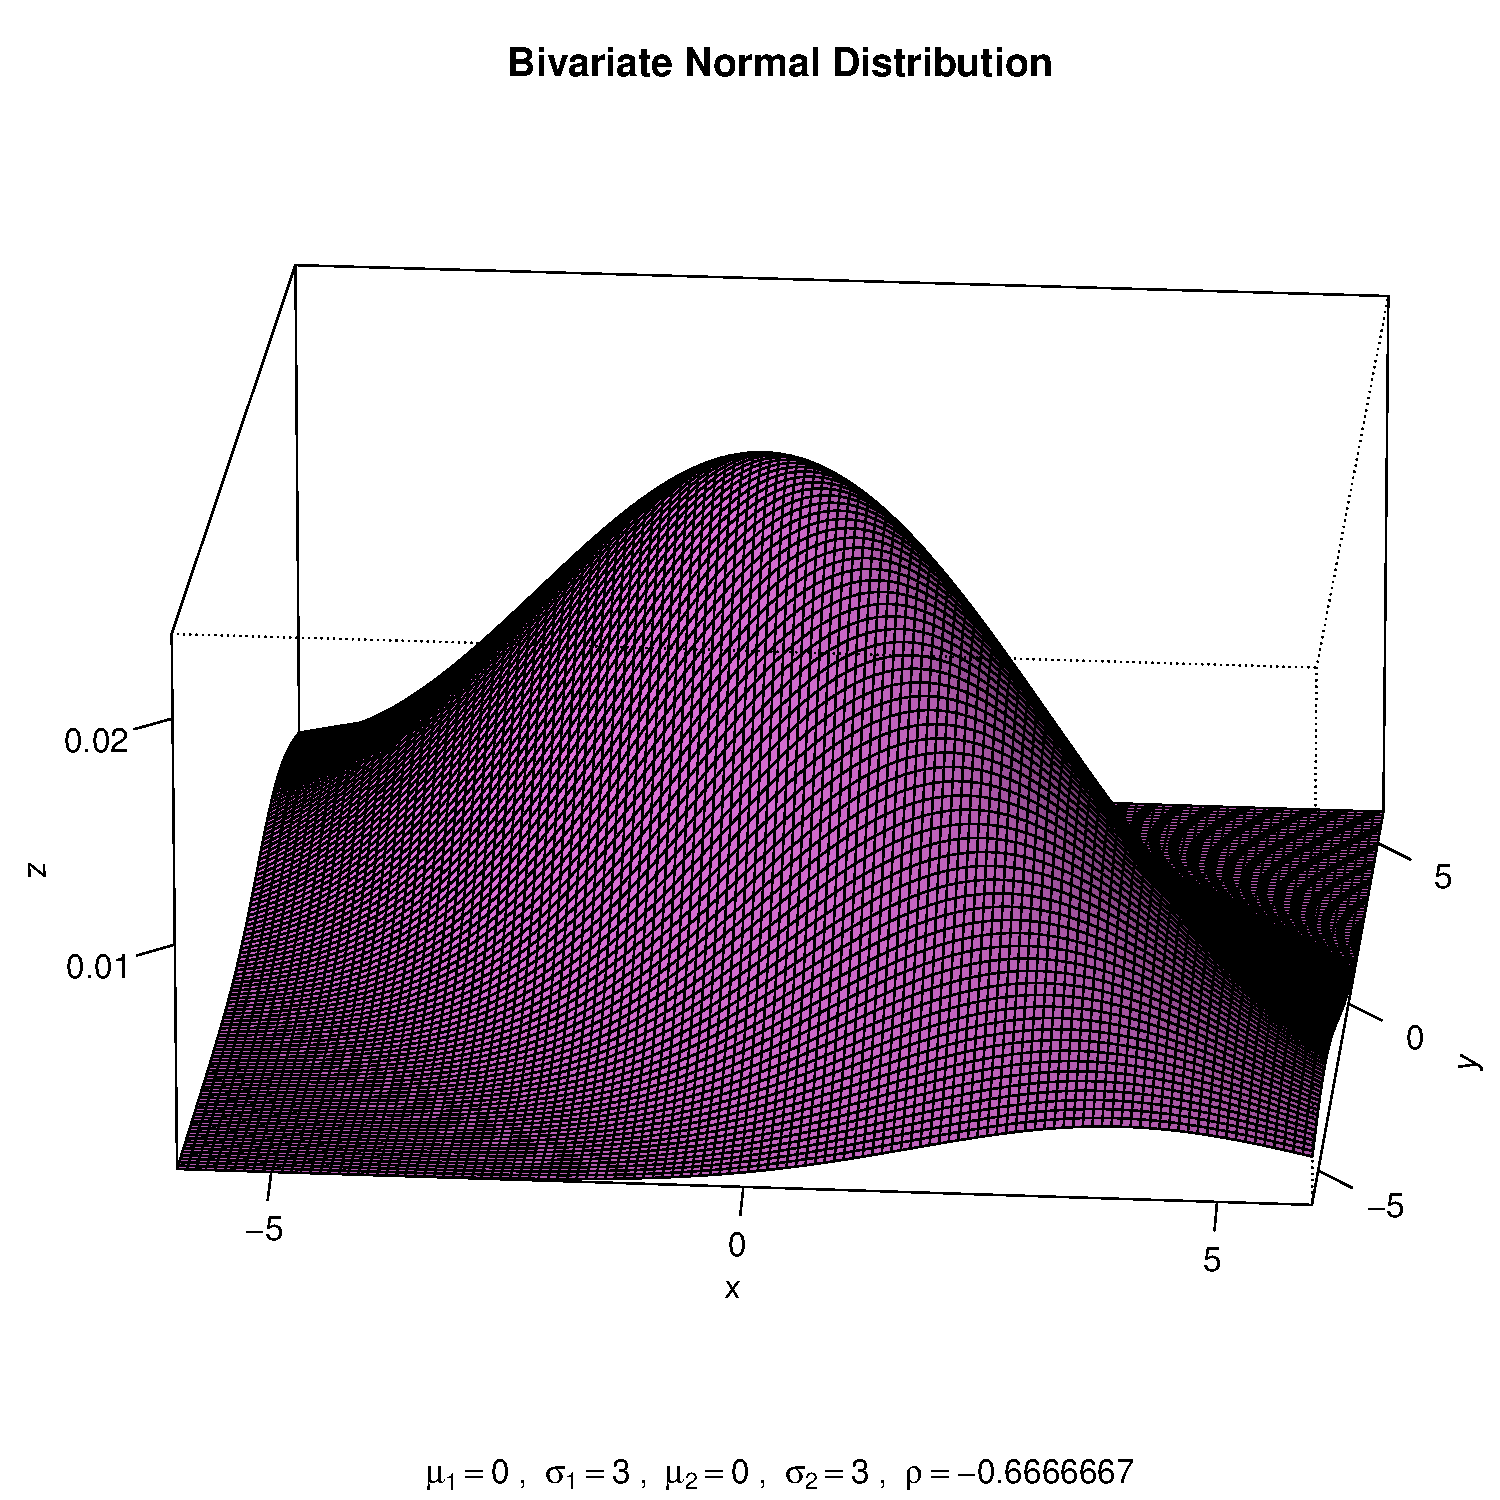
\includegraphics[scale=.25]{./Figures/F21.pdf}%
\figcaption{The density function of $\rv{X}$ as a surface over $\mathbb{R}^2$.}
\end{minipage}

\vspace{.5cm}


\begin{minipage}{.8\linewidth}
\centering%
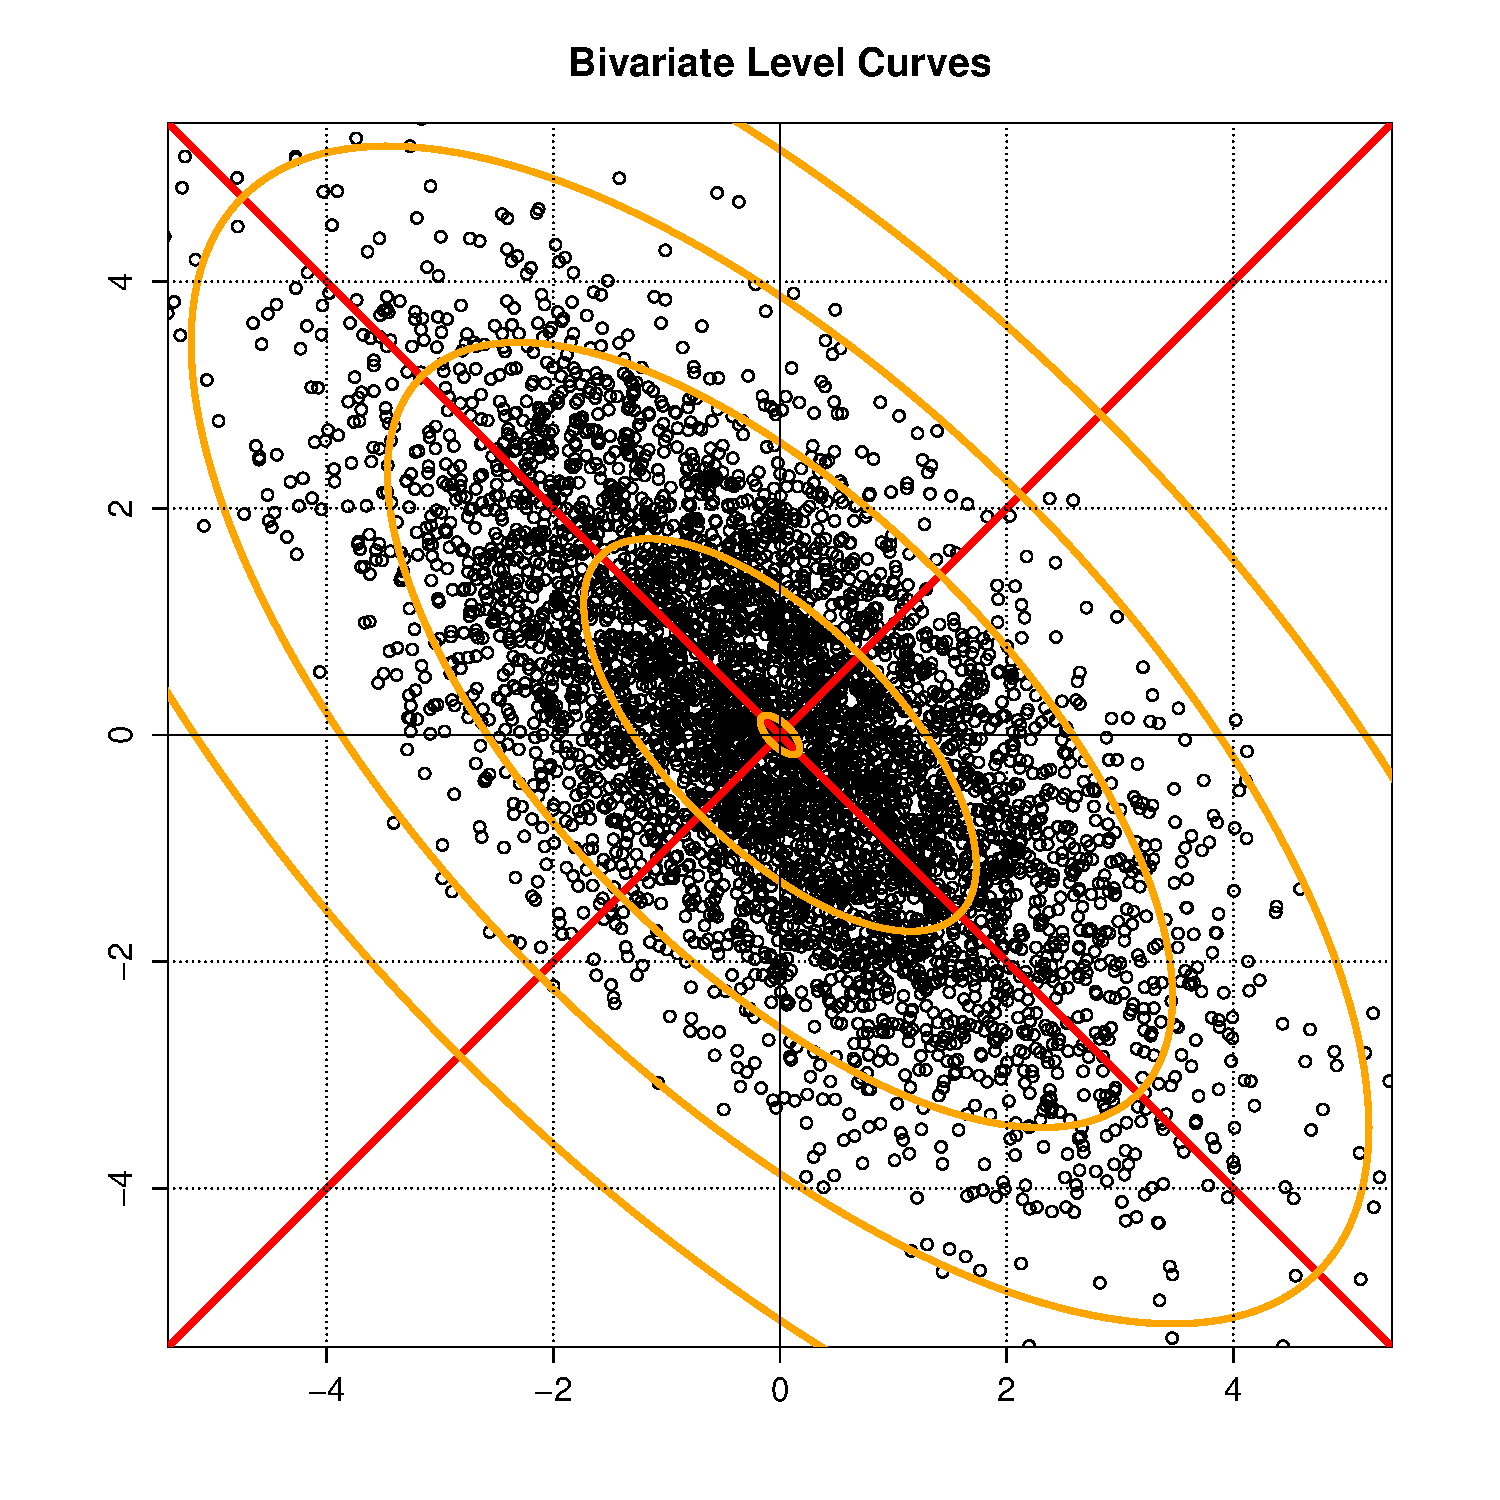
\includegraphics[scale=.25]{./Figures/F22.pdf}%
\figcaption{A sample of $n=5000$ from $\rv{X}$ overlain with the principal axes (red) and level curves of $\phi$ (orange).}
\end{minipage}
}

\subsection{The Degenerate $\Sigma$}

Now thus far we have assume that $\Sigma>0$ and so that $0$ wasn't an eigenvalue of $\Sigma$. However singular covariance matrices come up in practice as well as in theory so it is worth briefly addressing them. 

The idea behind a degenerate $p \times p$ covariance structure is that all of the action is happening in some subspace of $\mathbb{R}^p$. A singular covariance matrix means there is some linear relationship among the columns and thus there is some linear relationship among the variables. This means that some linear combination has a a correlation of $1$. Thus we aren't really in a $p$ dimensional space because we don't really have $p$ independent variables. Instead if $rank(\Sigma)=k<p$ then we only have $k$ variables giving us different information and thus anything we sample from this distribution is going to lie in some subspace. Furthermore if $\Sigma$ is close to being degenerate (some of the eigenvalues are quite small) then this will be approximately true and \emph{most} of the action will be contained in some subspace. This will be an important concept to keep in mind. 

If $0$ is an eigenvalue corresponding to some eigenvector $u$ of $\Sigma$ then the variance $\rv{X}$ in that direction, $u^T\rv{X}$, is zero and thus the length of the principal axis in that direction is zero. Thus instead of having true $p$--dimensional ellipsoids of concentration we have degenerate ones that line entirely in some proper subspace. The problem for defining a density function as before is that a distribution $\rv{X}\sim N_p(\bs{\mu},\Sigma)$ has zero density when viewed as a $p$--dimensional random vector because it lies in some subspace.

We can remedy this problem by ignoring the null space of $\Sigma$. We aren't really loosing anything because $Nul(\Sigma)$ has no variance. Thus if $rank(\Sigma)=k<p$ we can view $\rv{X}$ as a $k$--dimensional random vector with support in the affine subspace 
$$
\bs{\mu}+Row(\Sigma)=\{{\bf x}\in\mathbb{R}^p \mid {\bf x}=\bs{\mu}+{\bf y}\text{ for }{\bf y}\in Row(\Sigma)\}.
$$
By considering just those vectors in $\bs{\mu}+Row(\Sigma)=\bs{\mu}+Col(\Sigma)$ then we can define the density function for $\rv{X}$ as
$$
\bs{\phi}({\bf x})=\frac{1}{\sqrt{(2\pi)^k|\Sigma|_+}}\text{exp}\left(-\frac{1}{2}({\bf x}-\bs{\mu})^T\Sigma^+({\bf x}-\bs{\mu}))\right)
$$
for ${\bf x}\in\bs{\mu}+Row(\Sigma)$. Note that $|\Sigma|_+$ is the pseudo-determinant of $\Sigma$ defined by the product of its non-zero eigenvalues and $\Sigma^+$ is the pseudoinverse of $\Sigma$ as previously discussed and $rank(\Sigma)=k$.

We aren't going to go into great detail about such degenerate normal distributions. All we need really note is that our entire previous conversation essentially maps directly to these distributions when considering them under the restricted domain of support. This claim is justified more or less \emph{entirely} because if ${\bf x}\in\bs{\mu}+Row(\Sigma)$ then ${\bf x}-\bs{\mu}\in Row(\Sigma)$ and so $\Sigma^+=\Sigma^{-1}$ for these ${\bf x}-\bs{\mu}\in Row(\Sigma)$. 

%\section{Principal Components Analysis}

%\subsection{Basic Idea}
%\subsection{Correlation Among Components}
%\subsection{Variance Maximization}
%\subsection{Best Low-Rank Approximation}

%\section{Examples}
%\subsection{Classical PCA}
%\subsection{Finding Interesting Projections}











%%%%%%%%%%%%%%%%%%%%%%%%%%
\chapter{The CUR Algorithm}

\section{Definition and Uses of CUR}

The purpose of this chapter is threefold. First we will introduce the CUR matrix decomposition and associated CUR algorithm as they are presented in the literature. Secondly we will discuss a vision for how we might apply the algorithm to ameliorate some problems with principal components analysis. Lastly we will introduce an implementation of the CUR algorithm in R code, discuss the parameters of the algorithm and explore how these parameters affect the algorithm's behavior.

\subsection{Definition in Literature}

As evidenced by the preceding two chapters principal components analysis is a method that draws heavily on the theory of linear algebra. Indeed PCA can be performed directly from the singular value decomposition of a suitably centered data matrix. The beauty and elegance of the linear algebra upon which PCA draws makes the method quite attractive from the eyes of a mathematician. However mathematical elegance does not always translate into data-analytic simplicity. The structure of the principal components generated by PCA often causes statistical practitioners grief. To understand these problems let us first briefly review PCA. 

Throughout this discussion consider $X$ to be a variable-wise mean-centered $n \times p$ data matrix containing $n$ observations of a random vector $\rv{X}=(\mathscr{X}_1,\ldots,\mathscr{X}_p)^T$. Remember that the $i^{th}$ column of $X$ is the $n$ observations of $\mathscr{X}_i$. Thus in some sense $\mathscr{X}_i$ and $col(i,X)$ both represent a variable. However $\mathscr{X}_i$ is the \emph{random} variable whereas $col(i,X)$ is a collection of $n$ observations of this random variable.  Nonetheless they both have a right to be called a variable and are both, to some extent, an abstraction of the same feature of our data. The former $\mathscr{X}_i$ is the mathematical abstraction of the feature as a random variable whereas the latter $col(i,X)$ is the abstraction of the feature as a vector of observations. This is all to say that we will be referring to $col(i,X)$ both as a column of $X$ and as a variable of the data. The point is that there is a one-to-one correspondence between measured features of our data and columns of our data matrix and thus viewing the columns as variables is justified. 

We may generate principal components for the data directly from the first $r$ right singular vectors $\{{\bf v_i}\}_{i=1}^{r}$ of $X$ where $rank(X)=r$. Remember that we order both the right and left singular vectors of a matrix in decreasing order according to their associated positive singular values. Thus for $i=1,\ldots,r$ the $i^{th}$ principal component $PC_i$ is defined by  
$$
PC_i=X{\bf v_i}.
$$
Alternatively since the right singular vectors of $X$ are precisely the eigenvectors of the sample covariance matrix $S$ then we can define the $i^{th}$ principal components of $X$ as 
$$
PC_i=X{\bf v_i}
$$
where ${\bf v_i}$ is now the $i^{th}$ eigenvector of $S$. Again, for convenience we order the eigenvectors of any matrix in decreasing order according to their associated eigenvalues. 

While defining the principal components in terms of eigenvectors seems a mathematically nice definition it poses some interpretational problems for practitioners. To see this consider the situation in which a practitioner normally conducts PCA. First we collect data on some variables $\{\mathscr{X}_i\}_{i=1}^{p}$ and create observation vectors $\{col(i,X)\}_{i=1}^{p}$ comprising the columns of our data matrix $X$. Typically we have a good idea of how to interpret each column of $X$. After all these are observations we measured and so we can safely assume we know what we measured. In a scientific setting the variables that are the columns of $X$ may be moles of chemical in a solution, pH of some media, radiation counts or the like. Similarly in a social science setting the $\{col(i,X)\}$ may be something like socio-economic status, income level, anxiety level etc. Regardless of the domain from which the data comes the columns of $X$ generally have a relatively straight forward contextual interpretation. 

Principal components analysis can be thought of as re-expressing our data in a new set of variables. To begin with we have the data matrix $X$ which expresses our data column-wise as observation vectors of random variables $\{\mathscr{X}_i\}_{i=1}^{p}$. Principal components analysis re-expresses the data in terms of a new data matrix $D$. The columns of this data matrix $D$ express the data as observation vectors of a new set of random variables $\{\mathscr{PC}_i\}_{i=1}^{k}$ for $k \leq p$. The observation vectors of these random variables, and hence the columns of $D$, are precisely the principal components. Thus $col(i,D)=PC_i$ and so the columns of our new data matrix are precisely the $PC_i$ as described above. We change the variables we use to express our data from those of the columns of $X$ to the $PC_i$ comprising the columns of $D$. 

Hoping to use PCA to give us some insight into the data we would like to attach an interpretation to the principal components. After all, we had a nice interpretation of the columns of our original data matrix $X$ and so it would be nice to have an interpretation of the columns of our new data matrix $D$, the $\{PC_i\}_{i=1}^{k}$. However remember that the $i^{th}$ principal component is defined by
$$
PC_i=X{\bf v_i}=v_{1,i}col(1,X)+v_{2,i}col(2,X)+\cdots+v_{p,i}col(p,X)
$$
where $v_{j,i}$ is the $j^{th}$ component of the $i^{th}$ right singular vector of our data matrix $X$. Thus the columns of our new data matrix are the observations of the random variables
$$
\mathscr{PC}_i=v_{1,i}\mathscr{X}_1+v_{2,i}\mathscr{X}_2+\cdots+v_{p,i}\mathscr{X}_p.
$$

Unfortunately the ability to interpret the random variables $\mathscr{X}_i$ or equivalently the columns of $X$ in no way guarantees an ability to interpret linear combinations of them. After all, a linear combination is a mathematical idea not a physical one. Addition and multiplication are defined on vectors and random variables not physical objects. This poses a problem for principal components analysis because the principal components are linear combinations of the columns of $X$ and thus correspond to linear combinations of the $\mathscr{X}_i$. While we can get away with assigning meanings to the individual random variables $\mathscr{X}_i$ or the individual columns of $X$ often we get into hot water trying to attach meaning to a linear combination of either. 

This is not to say that we can never interpret the principal components nor are we saying that one should not try. We are simply noting that applying an interpretation to these linear combinations of $\{\mathscr{X}_i\}$, and thus linear combinations of the columns of $X$, is often difficult or impossible. Furthermore we should be careful about reifying these mathematical abstractions into meaningful objects. There is no guarantee that the mathematical abstractions of principal components represent any meaningful quantity at all.  

As an example consider measuring height, weight and income on a population of adults. If our first principal component is, say, 
$$
PC_1=\frac{1}{\sqrt{2}}(weight)+\frac{1}{\sqrt{2}}(height)
$$
then we may have a good intuition about what such a component means. We might interpret this first principal component as a variable measuring the ``size'' of a person. This is a case where we have a straightforward interpretation of the first principal component. However if our first principal component is
$$
PC_1=\frac{1}{\sqrt{14}}(weight)-\frac{2}{\sqrt{14}}(income)+\frac{3}{\sqrt{14}}(height)
$$
then a simple interpretation is not quite so easy.

Unfortunately a principal component in this latter form is the norm rather than the exception. Furthermore the problem is only exacerbated as the number of variables grows. Each principal component is typically a linear combination of all the variables. Thus generally the more variables we have measured, the more variables we will have to interpret in any given principal component. 

The inability to interpret principal components of a data set is troubling. PCA is a method which tries to see through the set of variables $\{col(i,X)\}$ we measured and find the true fundamental constituents of the data. It looks to find the set of components $\{PC_i\}$ which are the true underlying explanatory variables. Unfortunately while PCA can easily identify a set of variance-maximizing mutually uncorrelated variables we cannot usually make sense of the defining linear combinations in terms of the domain in which we are working. Thus we cannot see them as the true underlying physical generators of the data since they are not physical things at all. This is a very serious shortcoming of PCA as it fails to achieve precisely its intended goal.

It is at this point of failure in PCA which the CUR matrix decomposition enters the picture. For at least the past five years there has been research on a matrix factorization called the CUR matrix decomposition. The research has been led mainly by Michael Mahoney and Petros Drineas. In 2009 they published an article in the Proceedings of the National Academy of Sciences (PNAS) entitled ``CUR matrix decompositions for improved data analysis'' \cite{pnas}. This article was the starting point of my interest in the CUR matrix decomposition and the genesis of this research. 

In \cite{pnas} the CUR matrix decomposition is offered as a way to ameliorate some of the interpretational problems of PCA. The idea behind the CUR decomposition is as follows. Principal components analysis is a method which can be derived directly from the singular value decomposition of the data matrix $X$. Let's consider the singular value decomposition of the data matrix to be
$$
X=U\Sigma V^T.
$$
Now we previously discovered that if $r=rank(X)$ then the first $r$ columns of $U$ form a basis for the column space of $X$ and the first $r$ rows of $V^T$ form a basis for the row space of $X$. For principal components analysis we use the nice basis provided by the rows of $V^T$ to re-express the data. While from a mathematical viewpoint the rows of $V^T$ (equivalently the columns of $V$, the right singular vectors) are a nice basis in which to express the data matrix, concern is voiced in \cite{pnas} about their interpretability. A similar argument to the one above is made noting that the interpretational problems of PCA stem from structure of the principal components being linear combinations of the measured variables. 

However while it is not always possible to interpret the principal components of a data matrix it is also not always \emph{im}possible. Sometimes we can find a nice interpretation and sometimes we cannot. The crux of the issue is whether or not the weights on the variables in the linear combination lend themselves to an interpretation. Since the weights in the linear combinations defining our principal components are taken from the right singular vectors the root of the interpretational problems with PCA is identified in \cite{pnas} as the right singular vectors. That is, the problems in interpretation come from the fact that the components of the right singular vectors don't lend themselves to being interpreted. This, it is pointed out, should not be too surprising. After all, the right singular vectors are mathematical abstractions and nothing more. They are chosen for their mathematical properties not their data-analytic interpretability. 

With this in mind \cite{pnas} seeks to find an alternative to the right singular vectors. Instead of using the components from the right singular vectors as the weights in our linear combinations it is suggested we find a different set of weights that are (1) more interpretable and (2) can be used to create observation vectors that are almost as good as the principal components. Thus instead of creating a set of principal components $\{PC_i\}$ where
$$
PC_i=X{\bf v_i}=v_{1,i}col(1,X)+v_{2,i}col(2,X)+\cdots+v_{p,i}col(p,X)
$$
we could create a new set of observations $\{Y_i\}$ that do almost as well as the principal components in describing the data but where
$$
Y_i=a_{1,i}col(1,X)+\cdots+a_{p,i}col(p,X)
$$
and the $a_{j,i}$ are chosen such that the $Y_i$ are interpretable. 

The question is how we choose the $a_{i,j}$ so that we can create a new set $\{Y_i\}$ meeting the above criteria. To answer this \cite{pnas} proposes we do the following. Let us choose $w$ rows $\{R_i\}_{i=1}^{w}$ of our data matrix $X$ such that the $\{R_i\}$ do about as good of a job as the right singular vectors $\{{\bf v_i}\}$ in capturing the important subspaces of our data. Here the $R_i$ are $p\times 1$ column vectors. That is, $R_i=row(j,X)^T$ for some $1 \leq j \leq n$. Remember that the first $r$ right singular vectors $\{{\bf v_i}\}_{i=1}^{r}$ form a basis for row space of $X$. Thus if we run PCA and retain $k$ principal components then we are retaining the information of our data in the subspace of $Row(X)$ spanned by the first $k$ right singular vectors $\{{\bf v_i}\}_{i=1}^{k}$. The PNAS article \cite{pnas} proposes that we choose some rows of our data matrix whose span captures a subspace of $Row(X)$ that is about as good as that subspace spanned by the first $k$ right singular vectors. By ``about as good'' we mean that we don't lose much when we project the data down onto these rows. That is, if $R$ is our matrix having as its rows the chosen rows of our data matrix $X$, then
$$
||X-XR^T(R^+)^T||_F \approx ||X-XV_kV_k^T||_F
$$
where $V_k$ is the $p \times k$ matrix composed of the first $k$ columns of $V$. Note that $XR^T(R^+)^T$ is the projection of the rows of $X$ onto the rows of $R$, and $XV_kV_k^T$ is the projection of the rows of $X$ onto the columns of $V_k$ (i.e. the rows of $V_k^T$). 

The approach in \cite{pnas} is then to replace the right singular vectors, or ``eigenrows'', of our data matrix with a careful selection of rows from $X$. The hope is that the rows are more interpretable than the right singular vectors. That is, while linear combinations with weights from the right singular vectors do not make particularly interpretable principal components hopefully linear combinations of the columns of $X$ using the weights from the rows of our data matrix can be interpreted. Generally the idea is that any row of our data matrix $X$ corresponds to some concrete measurement of the variables $\mathscr{X}_1,\ldots,\mathscr{X}_p$. Thus the proposed vector
$$
Y_i=XR_i=r_{1,i}col(1,X)+r_{2,i}col(2,X)+\cdots+r_{p,i}col(p,X)
$$
can possibly be interpreted as a measure of being similar to the $i^{th}$ row. Let's explore this claim a little further.

The main idea of PCA is to find a set of fundamental constituents $\{PC_i\}$ that are the true underlying explanatory variables generating our data. We want to replace our original set of columns (observations of the variables) $\{col(i,X)\}$ with a new smaller set of representative observations $\{PC_i\}$ of the latent variables $\{\mathscr{PC}_i\}$. The problem with PCA is that often these ``fundamental constituents'' may not map nicely into any meaningful process generating the data. On the other hand replacing the columns of $X$ with the observation vectors $\{Y_i\}$ proposed in \cite{pnas} is using a set of ``fundamental constituents'' derived from actual measurements of our data. Thus to the extent that we can interpret any row of our data to be a proxy for some fundamental characteristic of the data set we have a nice interpretation. This is all still quite abstract so consider the following example. 

Assume we have a data set in which the measurements (rows) each fall into exactly one of three groups $G_1,G_2$ or $G_3$. Each measurement consists of values for each of the $p$ variables $\mathscr{X}_1,\ldots,\mathscr{X}_p$. Let's assume that the groups are well separated to begin with. If we run a principal components analysis on this data then we will hopefully be able to separate the groups when expressing our data using $k<p$ principal components $PC_1,\ldots,PC_k$. If we can do this then we can use the set of principal components $\{PC_i\}_{i=1}^{k}$ in place of the original set observation vectors $\{col(i,X)\}_{i=1}^{p}$. If the principal components represent the original data well then we would like to view them as observations of a set of ``unseen'' latent variables $\{\mathscr{PC}_i\}$. Unfortunately these principal components often lack a contextual interpretation. Thus it is hard to interpret them in terms of the contextual data-generating phenomena in which we are ultimately interested. The CUR method offers a better approach. Instead let us choose some representative rows of our data and use them to create a set of observation vectors $\{Y_i\}$ that are observations of the true underlying constituents of our data. In this case the most natural choice would be to choose one row in each group $G_1,G_2$ and $G_3$. Then if $R_i,R_j,R_m$ are, respectively, rows chosen from $G_1,G_2$ and $G_3$ then each of the variables 
$$
XR_i\,\text{,  }XR_j\text{ and }XR_m
$$
can be interpreted as observations of variables representing of one of the three groups. Thus our ``fundamental constituents'' each correspond to some group in the data. Another way to think of the above example is that instead of using $\{{\bf v_i}\}_{i=1}^{k}$ as a basis for our observations we use the set $\{R_i,R_j,R_m\}$ as our ``basis'' for the data. Instead of representing the observations in an uninterpretable basis of the ${\bf v_i}$ we represent them in a ``basis'' where each vector represents similarity to one of the groups.  Note that using the CUR method we have largely achieved the same goal to which PCA aspires. We have re-represented our data in a smaller number of constituents. Furthermore each constituent is interpretable as some fundamental underlying characteristic of the data. 

Now we still have yet to discuss precisely how we find these rows such that 
$$
||X-XR^T(R^+)^T||_F \approx ||X-XV_kV_k^T||_F.
$$
A significant contribution of \cite{pnas} is the algorithm to find the rows to do this. That is, to find rows of our data matrix $X$ which we can substitute for right singular vectors. We will call the algorithm to do this the CUR algorithm. In \cite{pnas} the algorithm is described as taking two parameters $k$ and $\epsilon$. The algorithm tries to choose rows of the data matrix $X$ that mostly sit in the span of the first $k$ right singular vectors. The hope is that these rows will then do about the same job as these right singular vectors. That is, they will capture a subspace that is about as good. How the algorithm chooses the rows will be the bulk of this chapter's material and precisely how well these rows perform in replacing the right singular vectors is, essentially, the contribution of this thesis. Thus we will not delve deeper into the nuts and bolds of the algorithm at the moment. That discussion will consume the remainder of the chapter.

 While we have described the CUR algorithm as an algorithm to select the rows of our data matrix it is actually a little more general than this. The above discussion is our best attempt to give a faithful representation of the literature on CUR's application to fixing interpretational problems with PCA. However to be fair \cite{pnas} presents the CUR algorithm as more than just an algorithm to do a PCA-like procedure. Rather  the algorithm is presented as a way to create a SVD-like decomposition. This is the CUR decomposition that we have alluded to but not yet directly discussed. Let us discuss it now. 

As noted earlier PCA is a method based wholly on the singular value decomposition of the data matrix $X$. Instead of using the SVD to decompose our data matrix into the product of $U$, $\Sigma$, and $V^T$ as $X=U\Sigma V^T$ the CUR decomposition approximately decomposes the $X$ matrix into the product of three matrices $C$, $U$ and $R$ such that
$$
X\approx CUR.
$$ 
The $C$ matrix contains a small number of columns from $X$, the $R$ matrix contains a small number of rows of $X$ and the matrix $U$ is the product of their Moore-Penrose pseudoinverses with $X$. That is, $U=C^+XR^+$. The $U$ matrix simply tries to keep the product $CUR$ close to $X$. The $C$ and $R$ matrices in CUR try to, respectively,  play the roles of $U$ and $V^T$ in the SVD. The $R$ matrix is precisely the same one we described previously and the $C$ matrix has an analogous construction. We form the rows of $R$ by trying to pick rows of $X$ that they approximately form a basis for the row space of $X$. Similarly we attempt to construct $C$ by choosing columns of $X$ that form an approximate basis for the column space of $X$. If we can do this then we can use the columns of $C$ in place of the left singular vectors, the eigencolumns, and the rows of $R$ in place of the right singular vectors, the eigenrows. Note that is precisely what we described above. When performing PCA one uses the weights from the $V$ matrix to construct the principal components. Using CUR one would instead use the weights from the $R$ matrix to construct our set $\{Y_i\}$ of observations of the latent variables. 

While the rows and columns of our data matrix will never be quite as parsimonious in spanning the important subspaces as the right and left singular vectors we will hopefully gain interpretability where we lose precision. To get an idea of just how much precision we lose a proof of error bounds on the decomposition is provided in \cite{pnas}. If we run the CUR algorithm with parameters $k$ and $\epsilon$ and get a CUR decomposition of $X\approx CUR$ then with high probability
$$
||X-CUR||_F\leq (1+\epsilon)||X-X_k||_F
$$
where $X_k$ is the best rank $k$ approximation to $X$.

\subsection{A Vision for CUR}

We are looking to apply the CUR algorithm to achieve something similar to PCA but with a stronger guarantee of interpretability. The approach described in the literature is to replace the columns of $X$ with vectors
$$
XR_i
$$
for some row $R_i$ of $X$ chosen by CUR. We use these variables instead of looking at the principal components of the data 
$$
X{\bf v_i}
$$
for some right singular vector ${\bf v_i}$ of $X$. The efficacy of this approach relies on two things being true. First we need the CUR algorithm to be able to pick the appropriate rows. That is, instead of running PCA and retaining $k$ principal components we can run CUR and pick off $w$ rows $\{R_i\}_{i=1}^{w}$ to create observation vectors $\{XR_i\}_{i=1}^{w}$ that do almost as good a job as the first $k$ principal components. Secondly we need these $\{XR_i\}$ to be more interpretable than the principal components. 

The first claim is covered to a large extent by the error bounds proven in \newline\cite{pnas}. However we need not concern ourselves with it too much at the moment. Rather let us critically look at the second claim. This second claim is that these new $\{XR_i\}$ are more interpretable than the principal components. Unfortunately, as pointed out in \cite{pnas}, these $\{XR_i\}$ are only interpretable to the extent that the rows $R_i$ are interpretable as representing some underlying characteristic of the data. 

In our previous example with the three groups $G_1,G_2,$ and $G_3$ we claimed that we could interpret $XR_i,XR_j$ and $XR_m$ each as representatives of one of the three groups. While a valid claim for the particular example,is in what  making such an interpretation is generally not an easy thing to do. It is not easy to interpret a row as being a representative of some underlying structure in the data. In our example we were able to do this only because we knew that each of $R_i,R_j$ and $R_m$ were indicative of the group structure in the data. 

We typically run PCA on data in a more exploratory manner. Generally we don't, \emph{a priori}, know the structure. Rather we run PCA to get a sense of the structure. Consider running CUR on some data whose structure is unknown. CUR will pick some row $R_i$ which we will use to construct a new observation vector $XR_i$. Our interpretation is that $XR_i$ is a measure of ``being like $R_i$''. CUR has said that the observation vector $XR_i$ is representative of some fundamental underlying structure in the data. However we don't generally know what structural characteristic of the data represented. We don't know what it means to be like $R_i$ unless we have some insight as to what underlying characteristic this $R_i$ is a representative. Thus generally we are at a loss for its interpretation. This should seem like a familiar problem. It is precisely the problem we originally had with PCA. We found principal components that were indicative of some underlying structure of the data. However we were then tasked with assigning a contextual interpretation to the underlying structure the component represented. Thus the CUR approach as defined in the literature seems to be plagued with some of the exact same problems it is trying to fix. 

Faced with these problems we abandon the application of CUR as described in the literature. As an alternative we consider an alternative application of Mahoney's work to solving the interpretational problems of PCA. After careful consideration of the CUR algorithm and criticisms voiced above it seems to be that as an alternative to PCA the most useful way to think about the CUR algorithm is as a variable selection algorithm. The remainder of this section will introduce our take on CUR's application in a PCA-like manner. 

The main contribution of the CUR algorithm is the way in which it chooses the columns and rows to construct $C$ and $R$ respectively. It attempts to pick columns and rows of $X$ that can be used in place of the eigencolumns and eigenrows of $X$. Remember that the $i^{th}$ column of $X$ corresponds to the $n$ observations of one of our measured variables $\mathscr{X}_i$. Thus as we are looking to use CUR to select variables then we are most interested in the columns CUR chooses.  

In a sense we are inverting the approach from the literature. Instead of focusing on choosing rows we focus on choosing columns. Indeed we are pretty much exclusively interested in having CUR select the important columns. Thus we will henceforth view the CUR algorithm as essentially a column selection algorithm. Given a real $n \times p$ data matrix $X$ for some $m \leq p$ CUR returns to us a $n \times m$ matrix $C$ whose $m$ columns are a subset of the columns of $X$. The question is in what manner selecting variables is analogous to PCA. While at first it may not seem very analogous we argue that at a high level selecting a subset of variables and running PCA move towards the same end. 

The end goal of principal components analysis is twofold. Not only would we like to attain a new set of variables that are the latent, unmeasured yet truly fundamental descriptors of the data. We would also like to have fewer principal components than our original set of variables. The hope is that by selecting the more parsimonious set of principal components we can cut through the redundancy of the originally measured variables and have a simpler, lower dimensional representation of our data.  

Consider having $p$ variables of interest. If we have a sample of size $n$ of the collection of $p$ random variables then we can create an $n \times p$ centered data matrix $X$. For a specified $k \leq rank(X)$ the PCA procedure takes this data matrix $X$ and returns a new set of $k$ observation vectors called principal components. We start with a set of $p$ columns $\{col(i,X)\}_{i=1}^{p}$ of $X$ that are observations of variables $\{\mathscr{X}_1,\ldots,\mathscr{X}_p\}$ and we have as output from PCA a new set of $k$ observation vectors 
$$
\{PC_1,\ldots,PC_k\}
$$
which measure the latent variables
$$
\{\mathscr{PC}_1,\ldots,\mathscr{PC}_k\}.
$$
As we often choose $k<rank(X)$ the set of principal components will generally only partially capture the original data. However the idea is that we can move from perfectly describing our data in terms of the $p$ columns of $X$ to approximately describing our data using a smaller set of $k$ principal components $PC_1,\ldots,PC_k$. These principal components are not usually observations of variables we have directly measured but can be thought of as observations of ``unseen'', latent variables underlying the data's fundamental structure. The dimensionality reduction afforded by PCA is traded for accuracy of our description of the data. 

At a very high level our application of CUR as a variable selection algorithm is doing something similar. Consider the same set of random variables $\{\mathscr{X}_1,\ldots,\mathscr{X}_p\}$. If we have, again, an $n \times p$ data matrix of samples associated with these variables then we can run the CUR algorithm on this data matrix. The CUR algorithm will return a subset of the columns of $X$ that it thinks are important to describing the data. Thus we start with a set of $p$ columns $\{col(i,X)\}_{i=1}^{p}$ as our input to CUR and have as output a subset of $m$ of these columns
$$
\{col(N_1,X),\ldots,col(N_m,X)\}
$$
where $1\leq N_1 < N_2 < \cdots < N_m \leq p$. The idea is that we can move from perfectly describing our data in terms of the $p$ columns of $X$ we measured to approximately describing the data using a subset of $m \leq p$ of these columns. Again, the simplicity that comes with reducing the number of observed variables comes as a trade-off with the fidelity with which we can reconstruct the original data. After all if we use CUR to select a subset of the columns then we are throwing away information in those columns we don't select. 

Note however that the interpretation of the variables selected by CUR is immediate. After all, they are a subset of the columns of $X$ and we know how to interpret the columns of $X$. Thus using CUR as a variable selection algorithm will not create interpretational problems in the same way PCA does. 

\subsection{The R Implementation}

We have now introduced the CUR algorithm both as it is described in the literature and as a variable selection algorithm applicable in a PCA-like manner. Our main goal with this paper is to give an empirical evaluation of this second formulation of CUR. However to understand the empirical behavior of CUR we need to understand precisely how the algorithm works. Thus we would like to discuss some of the nuts and bolts of the CUR algorithm. 

To carry out our empirical evaluations we will need an implementation of the CUR algorithm in code. Luckily one such implementation already exists. A 2012 article ``rCUR: an R package for CUR matrix decomposition'' appearing in BMC Bioinformatics offers an implementation of CUR. The article, henceforth \cite{biomed}, introduces a version of the CUR algorithm written in R code\footnote{\href{http://www.r-project.org/}{http://www.r-project.org/}}. The implementation is called rCUR.

We choose this rCUR implementation for our empirical work because it seems to be the official implementation of the CUR algorithm.\footnote{We are using version 1.3 of rCUR as updated on 2012-07-02. We found an error in the previous version's calculation of the leverage scores.} Initially we made this assumption because of the overlap in authorship between the PNAS and BMC Bioinformatics articles. After exchanging email with Michael Mahoney our assumption seems to be correct. Mahoney regards rCUR as currently the best implementation of the CUR algorithm. As he is one of the primary authors on the PNAS paper this seems to confirm our initial assumption. 

While sanctioned by Mahoney the rCUR package deviates slightly from the description of CUR we have previously presented. That is, the two algorithms are not precisely the same. There is a gap between the CUR algorithm described in \cite{pnas} and the rCUR algorithm implemented in \cite{biomed}.  We would rather have had an implementation without such discrepancies. However as we are interested in empirical analyses we are constrained to use \emph{some} implementation. While slightly different than the canonical definition of CUR our choice of the rCUR code seems to us the most fair implementation with which to evaluate the CUR algorithm. From this point forward to the extent that the two algorithms differ we will abandon our previous description of CUR and adopt the algorithm used in the rCUR implementation. The remainder of this section will be a discussion to this end. 

In \cite{pnas} the CUR algorithm is described as taking an $n\times p$ data matrix $X$ and two parameters $k$ and $\epsilon$. However this is not true to our choice of implementation of the algorithm. Instead of having an error parameter $\epsilon$ the R implementation in \cite{biomed} has a different parameter denoted $c$. A description of our chosen implementation of CUR is then the following. The CUR algorithm takes an $n \times p$ data matrix $X$, two parameters $k$ and $c$ and returns a matrix $C$. The $m\leq p$ columns of $C$ are the columns (variables) of our data matrix $X$ that CUR has chosen as important. This is the description we will use henceforth. Unless stated otherwise any future mention of the CUR algorithm will refer to this description. Thus we will think of the CUR algorithm as a function of $X$, $k$ and $c$ returning to us a matrix $C$ that identifies the important columns of $X$. For reasons yet to be explored we will call the parameter $k$ the rank parameter and the parameter $c$ the column parameter. The ultimate goal of this chapter is then to identify the roles of the rank parameter $k$ and column parameter $c$ in the CUR algorithm.

In order to investigate the rank and column parameters we first need a general overview of how the CUR algorithm operates. Consider running the CUR algorithm on an $n \times p$ data matrix $X$ giving it a rank parameter and column parameter of $k$ and $c$ respectively. The first thing CUR will do is use the rank parameter $k$ and the data matrix $X$ to create a probability distribution over the columns of the matrix. That is, for the $i^{th}$ column $col(i,X)$ CUR associates a number $\ell_i$ such that the collection $\{\ell_i\}_{i=1}^p$ forms a probability distribution. These $\ell_i$ are called the leverage scores. Somehow they purport to capture importance of the column in the matrix. For now we will consider these a black box. We will discuss them at length in the last section of this chapter. For now all we need to know is that the $k$ parameter and the data matrix $X$ are used to compute these ``importance scores'' $\{\ell_i\}_{i=1}^{p}$. 

Now in the literature the algorithm is described as follows. Using the leverage scores the algorithm makes a pass over the columns and selects the $i^{th}$ column with a probability $\min\{c\ell_i,1\}$ where $c$ is the column parameter given to the algorithm. So the algorithm takes the leverage scores and scales them by our column parameter. If $c\ell_i<1$ then the algorithm chooses that column as important with probability $c\ell_i$. If $c\ell_i \geq 1$ then the algorithm always chooses that column as important (i.e. with probability 1). 

While this description is close to what actually happens it is not precisely how the implemented code runs. The R implementation of CUR always chooses at least one column as important. In the previous description there is room for the algorithm to choose no columns. The implementers of the algorithm did not want the algorithm to ever choose no columns and so they adjusted it. If the algorithm makes a pass over the columns and chooses no columns then the algorithm will go back and make another pass. It will continue to do this until it has chosen at least one column. 

In any case, once the algorithm has chosen a set of columns it creates a matrix $C$ whose columns are those selected columns. It then returns this matrix to us. \vspace{.5cm}

The steps of the CUR algorithm can be written as follows. 
\begin{enumerate}
\item Get data matrix $X$ and two parameters $c$ and $k$. 
\item Calculate the leverage scores $\{\ell_i\}_{i=1}^{p}$ using $X$ and $k$.
\item Make a pass over the columns of the matrix and keep the $i^{th}$ column with probability $min\{c\ell_i,1\}$.
\item If we have chosen at least one column return a matrix $C$ consisting of those chosen columns. If we have not chosen any columns then go back to step 3. 
\end{enumerate}

\section{The Column Parameter}

The literature tells us that this $c$ parameter affects how many columns are chosen. Loosely speaking CUR will choose about $c$ columns from $X$. This is somewhat intuitive since $c$ scales the probabilities with which we keep any column. If $c$ is large then the probability of keeping any column will generally be ``large'' and so we will expect to choose many columns. The purpose of this section is to make this intuition precise. 

While in any pass the CUR algorithm keeps the $i^{th}$ column with probability $min\{c\ell_i,1\}$ empirically we often have that $c\ell_i < 1$ for every column. Thus we generally keep each column with probability $c\ell_i$ since $min\{c\ell_i,1\}=c\ell_i$. For simplicity then we will first do our analysis under the assumption that $c\ell_i < 1$ for each column. Once we have worked out this first analysis we will relax our assumption and deduce what happens if there are possibly some columns such that $c\ell_i \geq 1$. 

\subsection{Assuming $c\ell_i < 1$}

We know that the CUR algorithm makes a pass over the columns and chooses each column with probability $\min\{c\ell_i,1\}=c\ell_i$ since we are assuming for the time being that $c\ell_i<1$. We know however that the CUR algorithm will not halt until it has chosen at least one column and so it will go back and make as many passes as necessary to ensure that at least one column is chosen. This behavior is described in steps 3 and 4 above. 

For simplicity let us first assume that the algorithm does not make multiple passes. That is, if it chooses zero columns on the first pass then it stops and returns no columns. While this is not how the algorithm behaves in practice it is useful to consider this case as a stepping stone to the full-blown algorithm. 

\subsubsection{Single Pass}
We can think of choosing or not choosing a column as a Bernoulli trial. Either we choose the column (success) or don't (failure). The probability of choosing column $i$ is $c\ell_i$. Remember we choose each column with probability $min\{c\ell_i,1\}$ and since we are assuming $c\ell_i~<~1$ then $min\{c\ell_i,1\}=c\ell_i$. Thus the probability of ``success'' in our Bernoulli trial is $c\ell_i$. Hence each decision to choose or not choose a column is a Bernoulli random variable with probability of success $c\ell_i$. Notationally we write $\mathscr{X}_i \sim Bern(c\ell_i)$ where $\mathscr{X}_i$ is the random variable representing either choosing the $i^{th}$ column ($\mathscr{X}_i=1$) or not ($\mathscr{X}_i=0$). 

The CUR algorithm is a process which iterates over the columns and makes decisions to choose or not choose each column. It is thus performing $p$ successive Bernoulli trials. The number of columns that CUR chooses is then the sum of the Bernoulli trials. Let $\mathscr{C}$ be the random variable indicating how many columns the algorithm chooses. Then 
$$
\mathscr{C}=\mathscr{X}_1+\mathscr{X}_2+\ldots+\mathscr{X}_p=\sum_{i=1}^{p}\mathscr{X}_i.
$$
We might be tempted to say that $\mathscr{C}$ has a binomial distribution. However this is not true because the probability of success for each $\mathscr{X}_i$ can be different. Nonetheless, we can still characterize $\mathscr{C}$ quite easily. 

\vspace{.5cm}{\bf Expectation} \vspace{.5cm}

Since expectation is a linear operator then 
$$
\text{E}[\mathscr{C}] = \text{E}\left[\sum_{i=1}^{p}\mathscr{X}_i\right]=\sum_{i=1}^{p}\text{E}[\mathscr{X}_i].
$$
So the expected value for $\mathscr{C}$ is simply the sum of expected values of the $\mathscr{X}_i$. Since these $\mathscr{X}_i$ have a Bernoulli distribution with success probability $c\ell_i$ then each has an expected value of $c\ell_i$. Thus our expectation is 
$$
\e{\mathcal{C}}=\sum_{i=1}^{p}c\ell_i=c\sum_{i=1}^p\ell_i=c
$$
where the last equality holds because $\{\ell_i\}_{i=1}^{p}$ forms a probability distribution and thus sum to $1$.

This result is really quite nice. This is saying that the column parameter $c$ really does control how many columns are chosen in a precise probabilistic  manner. The expected number of columns to be chosen is $c$ the ``column parameter'' we give the CUR algorithm. 

\vspace{.5cm}{\bf Variance}\vspace{.5cm} 

Can we go further in characterizing how many columns are chosen? What we might also like to know is how much variability we will see in the number of columns chosen. This is also not a hard calculation. 

If we assume that the $\mathscr{X}_i$ are independent then variance is a linear operator over their sum. Since the $\mathscr{X}_i$ are separate Bernoulli trials then there is every reason to assume independence and so
$$
\text{var}\left[\mathscr{C}\right]=\text{var}\left[\sum_{i=1}^{p}\mathscr{X}_i\right]=\sum_{i=1}^{p}\text{var}\left[\mathscr{X}_i\right].
$$ 
The variance of a Bernoulli random variable $\mathscr{Y} \sim Bern(k)$ is $k(1-k)$ where $k$ is the probability of success. Thus the variance of each of our individual Bernoulli trials $\mathscr{X}_i$ is $c\ell_i(1-c\ell_i)$ because the probability of success is $c\ell_i$. Using this, the above variance then becomes 
$$
\begin{aligned}
\text{var}\left[\mathscr{C}\right]&=\sum_{i=1}^{p}c\ell_i(1-c\ell_i)\\
&=c\sum_{i=1}^{p}(\ell_i-c\ell_i^2)\\
&=c\left(\sum_{i=1}^{p}\ell_i-c\sum_{i=1}^{p}\ell_i^2\right)\\
&=c\left(1-c\sum_{i=1}^{p}\ell_i^2\right)\\
&=c-c^2\sum_{i=1}^{p}\ell_i^2.
\end{aligned}
$$
While not as intuitive as the formula for expectation we have still derived a relatively simple form for the variance. 

\subsubsection{Multiple Passes}

Now let us relax the assumption that we only make one pass over the columns. In reality the algorithm will repeat the selection process as many times as necessary to choose a least one column. Thus we perform $p$ Bernoulli trials and if none of them are successes we go and do $p$ more trials. We keep going back and doing $p$ more trials until we get a success.

As previously let $\mathscr{X}_i$ be a random variable representing either choosing the $i^{th}$ column or not. We still have that $\mathscr{X}_i$ is a Bernoulli random variable, however calculating its probability of success has become more complicated. Let $\mathscr{X}_i \sim Bern(p_i)$ such that $p_i$ is our probability of success. A first goal in calculating expectation and variance is to to calculate a value for $p_i$. 

To aid us in this goal let us also define the random variable $\mathscr{Z}$ to be the waiting time until we choose at least one column. That is $\mathscr{Z}$ is the number of times we have to ``reboot'' the choosing process. It is the number of passes choosing no columns before we finally choose at least one column in a pass. For example, if we choose a least one on the first attempt then $\mathscr{Z}=0$. If we make three passes over the columns choosing none and it isn't until the fourth attempt that we choose at least one column then $\mathscr{Z}=3$. 

Now let us compute  $P(\mathscr{X}_i=1)$, the probability of choosing column $i$. To do this we will use the Law of Total Probability partitioning the sample space with the countably infinite set
$$
\{Z=j \mid j=0,1,2,\ldots\}.
$$
Then we have that
\begin{align}
P(\mathscr{X}_i=1)&=P(\mathscr{X}_i=1 \cap \mathscr{Z}=0)+P(\mathscr{X}_i=1 \cap \mathscr{Z}=1)+\ldots\notag\\
&=\sum_{j=0}^{\infty} P(\mathscr{X}_i=1 \cap \mathscr{Z}=j)\notag\\
&=\sum_{j=0}^{\infty} P(\mathscr{X}_i=1 \mid \mathscr{Z}=j)P(\mathscr{Z}=j).\notag
\end{align}

In evaluating the product $P(\mathscr{X}_i=1 \mid \mathscr{Z}=j)P(\mathscr{Z}=j)$ the first thing to do is to evaluate $P(\mathscr{Z}=j)$. This is relatively easy since it is the probability that we choose no columns for the first $j$ passes. Indeed it is a geometric random variable since all selections in each pass and between different passes are independent and thus 
$$
P(\mathscr{Z}=j)=(p_0)^j(1-p_0)
$$
where $p_0$ is the probability of not choosing any column in a pass. It is easy to calculate $p_0$ since we have independence among Bernoulli trials in any pass and so
$$
p_0=\prod_{i=1}^{p}(1-c\ell_i).
$$
since the probability of keeping each column in a pass is $c\ell_i$. For the sake of keeping notation simple we will use $p_0$ henceforth to refer to this probability. We show how to calculate $p_0$ so that we are sure we are deriving a formula that can actually be evaluated. 

The last thing to do is look at $P(\mathscr{X}_i=1 \mid \mathscr{Z}=j)$. This is the probability that column $i$ was chosen and that we had to do $j$ passes before it was chosen. Let us define two new families of random variables. First define the family $\{\gamma_{i,j}\}$ where $\gamma_{i,j}$ is a Bernoulli random variable of choosing the $i^{th}$ column on the $j^{th}$ pass or not. Thus $\gamma_{i,j}\sim Bern\left(c\ell_i\right)$. Secondly define the family of random variables $\{\mathscr{W}_j\}$ where $\mathscr{W}_j$ is the number of columns chosen on the $j^{th}$ pass. Our claim is then that 
$$
P(\mathscr{X}_i=1 \mid \mathscr{Z}=j)=P(\gamma_{i,j+1}=1 \mid \mathscr{W}_{j+1}\geq 1).
$$
Note that the probability on the left size of the equation is the probability that we choose the $i^{th}$ column in any pass given that we first make $j$ unsuccessful passes before a successful $(j+1)^{st}$ pass. However if we first make $j$ passes without choosing any columns and choose the $i^{th}$ column on the $(j+1)^{st}$ pass then this is the same thing as choosing the $i^{th}$ column on the $(j+1)^{st}$ pass given that we choose some column on that pass. This is precisely the probability on the right hand side. 

Thus
$$
\begin{aligned}
P(\mathscr{X}_i=1 \mid \mathscr{Z}=j)&=P(\gamma_{i,j+1}=1 \mid \mathscr{W}_{j+1}\geq 1)\\
&=\frac{P(\gamma_{i,j+1}=1 \cap \mathscr{W}_{j+1}\geq 1)}{P(\mathscr{W}_{j+1}\geq 1)}\\
&=\frac{P(\mathscr{W}_{j+1}\geq 1 \mid \gamma_{i,j+1}=1)P(\gamma_{i,j+1}=1)}{1-P(\mathscr{W}_{j+1}=0)}
\end{aligned}
$$

Now $P(\mathscr{W}_{j+1}\geq 1 \mid \gamma_{i,j+1}=1)=1$ since if we choose column $i$ in the $(j+1)^{st}$ pass then we must choose at least one. We also know that $P(\gamma_{i,j+1}=1)=c\ell_i$ by construction. Finally then $P(\mathscr{W}_{j+1}=0)=p_0$ since this is just the probability that we choose no columns and is thus our failure probability. Hence
$$
P(\mathscr{X}_i=1 \mid \mathscr{Z}=j)=P(\gamma_{i,j+1}=1 \mid \mathscr{W}_{j+1}\geq 1)=\frac{c\ell_i}{1-p_0}
$$

%Firstly we look at $P(\mathscr{X}_i=1 \mid \mathscr{Z}=j)$.This is the probability that column $i$ was chosen and that we had to do $j$ passes before it was chosen. Note that this means we chose column $i$ precisely on pass $j+1$. We know that it cannot have been chosen on pass $1,2,\ldots,j$ since we are given that $\mathscr{Z}=j$ and so we know that in the first $j$ passes we picked no columns. Furthermore since we must have picked something in pass $j+1$ then the algorithm stopped after this pass. Since column $i$ was chosen in one of these $j+1$ passes but it wasn't chosen in the first $j$ then it must have been chosen in the $(j+1)^{st}$. Thus the probability that $\mathscr{X}_i=1$ given that $\mathscr{Z}=j$ is the probability that we choose column $i$ on pass $j+1$. 

%Next we notice that this probability has a certain type of memorylessness. The number of previous passes does not affect the probability of choosing each column in some later pass. Each pass is precisely identical as described by the algorithm. In each pass we keep column $i$ with the same probability $c\ell_i$. Thus given that we are \emph{precisely} in pass 5 as opposed to being \emph{precisely} in pass 500 does not affect the probability that we keep each column in each of those particular passes. Notationally we can write this as
%$$
%P(\mathscr{X}_i=1 \mid \mathscr{Z}=4)=P(\mathscr{X}_i=1 \mid \mathscr{Z}=499)=P(\mathscr{X}_i=1 \mid \mathscr{Z}=k)
%$$
%for any $k$. Furthermore we know that all of these probabilities are equal to $c\ell_i$ since given the fact that we are in some particular pass the probability of keeping column $i$ \emph{in that pass} is $c\ell_i$. Thus
%$$
%P(\mathscr{X}_i =1 \mid \mathscr{Z}=j)=c\ell_i. 
%$$
%To be clear, we are NOT saying that $\mathscr{X}_i$ is independent of $\mathscr{Z}$. This is not true. What we are saying is that each pass is identical and chooses each column with probability $c\ell_i$. The difference is that we are talking not about $P(\mathscr{X}_i=1)$ which is the probability of choosing column $i$ in any pass, we are talking about $P(\mathscr{X}_i=1\mid \mathscr{Z}=j)$, the probability of choosing column $i$ particularly in pass $j+1$. Given that we are operating in a particular pass the probability of choosing the $i^{th}$ column is $c\ell_i$ regardless which particular pass that happens to be. 



Since we now have expressions for both $P(\mathscr{X}_i = 1 \mid \mathscr{Z}=j)$ and $P(\mathscr{Z}=j)$ then we can calculate $P(\mathscr{X}_i=1)$ as
\begin{align}
P(\mathscr{X}_i=1)&=\sum_{j=0}^{\infty}P(\mathscr{X}_i=1 \mid \mathscr{Z}=j)P(\mathscr{Z}=j)\notag\\
&=\sum_{j=0}^{\infty}\left(\frac{c\ell_i}{1-p_0}\right)(\left(p_0)^j(1-p_0)\right)\notag\\
&=\sum_{j=0}^{\infty}c\ell_i(p_0)^j\notag\\
&=c\ell_i\sum_{j=0}^{\infty}(p_0)^j\notag\\
&=\frac{c\ell_i}{1-p_0}\notag
\end{align}
since $0<p_0<1$ makes the sum a convergent geometric series. This is precisely the $p_i$ for which we were previously searching. Thus we now we know how each of the $\mathscr{X}_i$ are distributed. 

An important point to note here is that we could use the same argument for finding $P(\mathscr{X}_i=1 \cap \mathscr{X}_k=1)$ for some $i\neq k$. The only point that changes is that 
$$
P(\mathscr{X}_i=1 \cap \mathscr{X}_k=1\mid \mathscr{Z}=j)=\frac{(c\ell_i)(c\ell_k)}{1-p_0}
$$
and so 
$$
P(\mathscr{X}_i=1 \cap \mathscr{X}_k=1)=\frac{(c\ell_i)(c\ell_k)}{1-p_0}.
$$
Indeed we could do this for any intersection of the $\mathscr{X}_i's$. Later we will have use of the intersection of two events and so it is worth pointing out that their probability can be arrived at via this argument.

Note also that the above shows that the $\mathscr{X}_i$ are not independent since 
$$
P(\mathscr{X}_i=1 \cap \mathscr{X}_k=1)=\frac{(c\ell_i)(c\ell_k)}{1-p_0}\neq \frac{(c\ell_i)(c\ell_k)}{(1-p_0)^2}=P(\mathscr{X}_i=1)P(\mathscr{X}_k=1).
$$
This is a somewhat unintuitive result since it says knowing that $\mathscr{X}_i=1$ tells us something about $P(\mathscr{X}_k=1)$. However it is a fact of life with this algorithm and important to keep in mind. 

\vspace{.5cm}
{\bf Expectation}
\vspace{.5cm}

Let us define $\mathscr{C}$ as previously such that
$$
\mathscr{C}=\sum_{i=1}^{p}\mathscr{X}_i.
$$

Then since expectation is a linear operator then
$$
\text{E}[\mathscr{C}]=\text{E}\left[\sum_{i=1}^{p}\mathscr{X}_i\right]=\sum_{i=1}^{p}\text{E}[\mathscr{X}_i].
$$
We know that $\mathscr{X}_i \sim Bern\left(\frac{c\ell_i}{1-p_0}\right)$ and so 
$$
\text{E}[\mathscr{X}_i]=\frac{c\ell_i}{1-p_0}
$$
meaning that
$$
\text{E}[\mathscr{C}]=\sum_{i=1}^{p}\frac{c\ell_i}{1-p_0}=\frac{c}{1-p_0}\sum_{i=1}^{p}\ell_i=\frac{c}{1-p_0}
$$
since the $\{\ell_i\}$ form a probability distribution and thus sum to $1$. 

Thus in comparison to the single-pass simplified algorithm originally presented the expectation for the number of columns CUR chooses is enhanced by $\frac{1}{1-p_0}$. We expect to choose slightly more than $c$ columns. 

\vspace{.5cm}
{\bf Variance}
\vspace{.5cm}

The variance is a little trickier than the expected value. We know that the variance of the sum of random variables is the sum of the covariances among all ordered pairs of the variables. For us this means
$$
\text{var}\left[\mathscr{C}\right]=\text{var}\left[\sum_{i=1}^{p}\mathscr{X}_i\right]=\sum_{i=1}^{p}\sum_{j=1}^{p}\text{cov}\left[\mathscr{X}_i,\mathscr{X}_j\right].
$$
Thus if we can determine the covariance between any two $\mathscr{X}_i$ and $\mathscr{X}_j$ then we know the variance.

Clearly for $i=j$ then 
$$
\text{cov}\left[\mathscr{X}_i,\mathscr{X}_j\right]=\text{cov}\left[\mathscr{X}_i,\mathscr{X}_i\right]=\text{var}\left[\mathscr{X}_i\right]=\frac{c\ell_i}{1-p_0}\left(1-\frac{c\ell_i}{1-p_0}\right)
$$
since $\mathscr{X}_i \sim Bern\left(\frac{c\ell_i}{1-p_0}\right)$.

When $i \neq j$ then we really must compute the covariance between two $\mathscr{X}$. We can rewrite the covariance using its ``shortcut'' formula as
$$
\text{cov}\left[\mathscr{X}_i,\mathscr{X}_j\right]=\text{E}[\mathscr{X}_i\mathscr{X}_j]-\text{E}[\mathscr{X}_i]\text{E}[\mathscr{X}_j].
$$
%\text{E}[{(\mathscr{X}_i-\text{E}[\mathscr{X}_i])(\mathscr{X}_j-\text{E}[\mathscr{X}_j])}]

The second term, $\text{E}[\mathscr{X}_i]\text{E}[\mathscr{X}_j]$, is easy to compute because we know the expectation for the $\mathscr{X}_i$. The first term is more difficult. Nonetheless we can still figure it out. We know that
$$
\text{E}[\mathscr{X}_i\mathscr{X}_j]=\sum_{x_1}\sum_{x_2}x_1x_2f(x_1,x_2)
$$
where $f$ is our joint distribution between $\mathscr{X}_i$ and $\mathscr{X}_j$. Since the sum is over $x_1=0,1$ and $x_2=0,1$ (since both are Bernoulli) then it is
$$
\text{E}[\mathscr{X}_i\mathscr{X}_j]=(0)(0)f(0,0)+(1)(0)f(1,0)+(0)(1)f(0,1)+(1)(1)f(1,1).
$$
and so we have a great simplification that 
$$
\text{E}[\mathscr{X}_i\mathscr{X}_j]=f(1,1)
$$
which shouldn't be too surprising given that they are both Bernoulli. Since 
$$
f(1,1)=P(\mathscr{X}_i=1 \cap \mathscr{X}_j=1)
$$ 
then we are done because we previously computed this to be
$$
\frac{(c\ell_i)(c\ell_j)}{1-p_0}.
$$

Putting this all together then 
$$
\text{cov}\left[\mathscr{X}_i,\mathscr{X}_j\right]=\frac{(c\ell_i)(c\ell_j)}{1-p_0}-\left(\frac{c\ell_i}{1-p_0}\right)\left(\frac{c\ell_j}{1-p_0}\right).
$$
and so
\begin{align}
\text{var}\left[\mathscr{C}\right]&=\sum_{i=1}^{p}\text{var}\left[\mathscr{X}_i\right]+\sum_{i=1}^{p}\sum_{i \neq j}\text{cov}\left[\mathscr{X}_i,\mathscr{X}_j\right]\notag\\
&=\sum_{i=1}^{p}\left(\frac{c\ell_i}{1-p_0}\left(1-\frac{c\ell_i}{1-p_0}\right)\right)+\sum_{i=1}^{p}\sum_{j\neq i}\left(\frac{(c\ell_i)(c\ell_j)}{1-p_0}-\left(\frac{c\ell_i}{1-p_0}\right)\left(\frac{c\ell_j}{1-p_0}\right)\right).\notag
\end{align}

This formula is rather dense so let's see if we can simplify it. First let's consider the variance term $\sum_{i=1}^{p}Var(\mathscr{X}_i)$. This term has the same form as our original variance term. To see this let $C=\frac{c}{1-p_0}$. Then
$$
\sum_{i=1}^{p}\text{var}\left[\mathscr{X}_i\right]=\sum_{i=1}^{p}C\ell_i(1-C\ell_i)=C-C^2\sum_{i=1}^{p}\ell_i^2.
$$

Let's see if we can make some similar simplifications to our covariance term 
$$
\sum_{i=1}^{p}\sum_{j\neq i}\left(\frac{(c\ell_i)(c\ell_j)}{1-p_0}-\left(\frac{c\ell_i}{1-p_0}\right)\left(\frac{c\ell_j}{1-p_0}\right)\right).
$$

First note that we can pull out any terms not dependent on $j$ to the outer summation and get
$$
\sum_{i=1}^{p}\frac{c\ell_i}{1-p_0}\sum_{j\neq i}\left(c\ell_j-\frac{c\ell_j}{1-p_0}\right).
$$
and further pulling out the remaining $c$ and $1-p_0$ getting
$$
\sum_{i=1}^{p}\frac{c^2\ell_i}{(1-p_0)^2}\sum_{j\neq i}\left(\ell_j(1-p_0)-\ell_j\right).
$$
which gives us
\begin{align}
&\sum_{i=1}^{p}\frac{c^2\ell_i}{(1-p_0)^2}\sum_{j\neq i}\left(\ell_j1-\ell_jp_0-\ell_j\right)\notag\\
&=\sum_{i=1}^{p}\frac{c^2\ell_i}{(1-p_0)^2}\sum_{j\neq i}\left(\ell_j-\ell_jp_0-\ell_j\right)\notag\\
&=\sum_{i=1}^{p}\frac{c^2\ell_i}{(1-p_0)^2}\sum_{j\neq i}-\ell_jp_0\notag\\
&=\sum_{i=1}^{p}\frac{-p_0c^2\ell_i}{(1-p_0)^2}\sum_{j\neq i}\ell_j\notag\\
&=\sum_{i=1}^{p}\frac{-p_0c^2\ell_i}{(1-p_0)^2}(1-\ell_i)\notag
\end{align}
where the last step holds since
$$
\sum_{i=1}^{p}\ell_i=1
$$
and so 
$$
\sum_{j\neq i}\ell_i=\left(\sum_{j=1}^{p}\ell_j\right)-\ell_i=1-\ell_i.
$$

We are free to pull out terms not dependent on $i$ and thus we can simplfy the sum to 
$$
\frac{-p_0c^2}{(1-p_0)^2}\sum_{i=1}^{p}\ell_i(1-\ell_i)=\frac{-p_0c^2}{(1-p_0)^2}\left(1-\sum_{i=1}^{p}\ell_i^2\right)
$$

Now let's pull back together our simplifications for the variance and covariance parts. If we let
$$
C=\frac{c}{1-p_0}\text{\quad and\quad }L^2=\sum_{i=1}^{p}\ell_i^2
$$
then we have 
\begin{align}
\sum_{i=1}^{p}\text{var}\left[\mathscr{X}_i\right]=C-(CL)^2\notag\\
\sum_{i=1}^{p}\sum_{i \neq j}\text{cov}\left[\mathscr{X}_i,\mathscr{X}_j\right]=-p_0C^2(1-L^2)\notag
\end{align}
meaning that
$$
\text{var}\left[\mathscr{C}\right]=C-(CL)^2-p_0C^2(1-L^2).
$$

While one might have hoped for a simpler expression for the variance this seems to be the correct calculation. 

\subsubsection{An Example}

Let us verify our theoretical work with an example. 

\ex{1}{

For this empirical example we use R to generate a centered $n \times p$ data matrix $X$ where $n=5000$ and $p=3$. The data matrix contains $5000$ observations of three random variables $\mathscr{A}_1,\mathscr{A}_2,\mathscr{A}_3$ that have a multivariate normal distribution such that $\rv{A}=(\mathscr{A}_1,\mathscr{A}_2,\mathscr{A}_3)\sim N_3({\bf 0},\Sigma)$ and $\Sigma=diag(1,1,1)$. 

We are going to run CUR on this data matrix with $k=1$ and $c=1$. For our particular matrix $X$ we calculate the leverage scores for the three columns to be 
$$
\ell_1=.9044,\,\ell_2=.02539,\,\ell_3=.0716.
$$
and thus since $c=1$ then $c\ell_i<1$ for $i=1,2,3$. We calculate 
$$
L^2=\sum_{i=1}^{3}\ell_i^2=.823
$$
and 
$$
p_0=\prod_{i=1}^{3}(1-c\ell_i)=.0865.
$$
Then
$$
\text{E}\left[\mathscr{C}\right]=C=\frac{c}{1-p_0}=\frac{1}{1-.0865}=1.0948
$$
and
$$
\text{var}\left[\mathscr{C}\right]=C-(CL)^2-p_0C^2(1-L^2)=.08934.
$$

We now run CUR $N=5000$ times and record how many columns have been chosen for each run. Doing this we find that the sample mean and variance are respectively
$$
M=1.0908
$$
and
$$
S^2=.08737.
$$
Thus our theoretical values seems to be borne our in the empirical running of the algorithm. 
}

\subsection{No Assumptions on $c\ell_i$}

The analysis thus far has used the assumption that the $c\ell_i$ are less than $1$. This however does not need to be the case. Indeed it is possible for some $c\ell_i$ to be greater than $1$. Let us see what happens when there is at least one $c\ell_i\geq 1$. 

If there is some column $i$ for which $c\ell_i \geq 1$ then the probability of choosing the associated column will be $1$. This follows because $min\{c\ell_i,1\} = 1$. Thus the associated expectation of the Bernoulli trial $\mathscr{X}_i$ is $1$ and its variance is $0$. This is true because $\mathscr{X}_i \sim Bern(1)$. Thus our previously calculated values for the expectation and variance of $\mathscr{C}$ need to be changed. Note however that since we always choose at least one column then we will always do one pass because we will always choose at least one column on the first pass. Thus the case where there is some $c\ell_i\geq 1$ is reminiscent of our first exploration where we assume the algorithm only makes one pass. 


\subsubsection{Expectation}
We know from the previous discussion that the expected value is 
$$
\text{E}[\mathscr{C}]=\sum_{i=1}^p\text{E}[\mathscr{X}_i].
$$
Let $\mathcal{S}$ be the set of trials $\mathscr{X}_i$ such that $c\ell_i \geq 1$ and $\mathcal{T}$ be the complementary set of $\mathscr{X}_i$ with $c\ell_i < 1$. Then our sum may we written as
$$
\text{E}[\mathscr{C}]=\sum_{\mathscr{X}_i \in \mathcal{S}}\text{E}[\mathscr{X}_i]+\sum_{\mathscr{X}_i \in \mathcal{T}}\text{E}[\mathscr{X}_i].
$$
As we said before $\text{E}[\mathscr{X}_i]=1$ for all $\mathscr{X}_i\in \mathcal{S}$ and so our sum becomes
$$
\text{E}[\mathscr{C}]=\sum_{\mathscr{X}_i \in \mathcal{S}}1+\sum_{\mathscr{X}_i \in \mathcal{T}}\text{E}[\mathscr{X}_i].
$$
If $|\mathcal{S}|=k < p$, i.e. there are $k$ variables such that $c\ell_i \geq 1$, then the sum further simplifies to
$$
\begin{aligned}
\text{E}[\mathscr{C}]&=k+\sum_{\mathscr{X}_i \in \mathcal{T}}\text{E}[\mathscr{X}_i]\\&
=k+c\sum_{\mathscr{X}_i \in \mathcal{T}}\ell_i.
\end{aligned}
$$

How does this expectation compare to our previous results for expectation? Since for $\mathscr{X}_i\in \mathcal{S}$ we have that $\text{E}[\mathscr{X}_i]=1\leq c\ell_i$ then 
$$
\sum_{\mathscr{X}_i \in \mathcal{S}}\text{E}[\mathscr{X}_i]\leq\sum_{\mathscr{X}_i \in \mathcal{S}}c\ell_i.
$$
This means that 
$$
\sum_{\mathscr{X}_i \in \mathcal{S}}\text{E}[\mathscr{X}_i]+\sum_{\mathscr{X}_i \in \mathcal{T}}\text{E}[\mathscr{X}_i]\leq\sum_{\mathscr{X}_i \in \mathcal{S}}c\ell_i+\sum_{\mathscr{X}_i \in \mathcal{T}}\text{E}[\mathscr{X}_i].
$$
The left-hand side here is simply $\text{E}[\mathscr{C}]$ while the right-hand side is $c\sum_{i=1}^{p}\ell_i=c$. Then 
$$
\text{E}[\mathscr{C}] \leq c  
$$
and since $c < \frac{c}{1-p_0}$ for any number $0<p_0<1$ we have
$$
\text{E}[\mathscr{C}] < \frac{1}{1-p_0}.
$$
Thus the expectation if some $c\ell_i \geq 1$ is $c$ which is smaller than we get if all $c\ell_i< 1$. 


Thus in summary, if we don't assume anything about the leverage scores $\ell_i$ or the columns parameter $c$, then the expectation is 
$$
\text{E}[\mathscr{C}]=k+c\sum_{\mathscr{X}_i \in \mathcal{T}}\ell_i
$$
where $k$ is the number of columns for which $c\ell_i \geq 1$ and $\mathcal{T}$ is the set of columns for which $c\ell_i < 1$. If we let $q=c\sum_{\mathscr{X}_i \in \mathcal{T}}\ell_i$ then the expectation is simply 
$$
\text{E}[\mathscr{C}]=k+q
$$
which is the expected number of columns chosen from those columns with a non-certain probability ($q$) plus the number of columns that must be chosen ($k$). 

\subsubsection{Variance}
The variance is even easier to characterize than the mean. 

Since we assume that the Bernoulli trials $\mathscr{X}_i$ are independent then our variance (as discussed before) is
$$
\text{var}\left[\mathscr{C}\right] = \sum_{i=1}^{p}\text{var}\left[\mathscr{X}_i\right]
$$
however now since $\text{var}\left[\mathscr{X}_i\right] = 0$ for columns which have $c\ell_i \geq 1$ then we can ignore these variances from our sum. Thus our variance simplifies to
$$
\text{var}\left[\mathscr{C}\right] = \sum_{\mathscr{X}_i \in \mathcal{T}}\text{var}\left[\mathscr{X}_i\right]
$$
where $\mathcal{T}$ is the set of $\mathscr{X}_i$ which have $c\ell_i < 1$. Thus all together then 
$$
\text{var}\left[\mathscr{C}\right] = c\sum_{\mathscr{X}_i \in \mathcal{T}}\ell_i-c^2\sum_{\mathscr{X}_i \in \mathcal{T}}\ell_i^2
$$

\ex{2}{

Let's consider our previous data matrix $X$ from example $1$. Now however we will run CUR with $c=2$. Now remember that the leverage scores for the columns are 
$$
\ell_1=.9044,\,\ell_2=.02539,\,\ell_3=.0716.
$$
and so 
$$
c\ell_1=1.8088,\,c\ell_2=.0507,c\,\ell_3=.1403.
$$

Note now that $c\ell_1 \geq 1$ and so we are now in the last case we just discussed. Thus we calculate the expectation and variance as 
$$
\text{E}\left[\mathscr{C}\right]=1+2(.0507+.1403)=1.19
$$
and
$$
\text{var}\left[\mathscr{C}\right]=2(.0507+.1403)-4(.0507^2+.1403^2)=.1688
$$

Note if we run CUR $N=5000$ times with $k=1$ and $c=2$ then we get sample mean and variance of 
$$
M=1.1996
$$
and
$$
S^2=.1769.
$$

Thus the empirical results seem to verify our original calculations. 
}

\subsection{Conclusions}

We would like to wrap up our discussion on the column parameter $c$ at this point. The thrust of this subsection was to determine what role the $c$ parameter plays in the CUR algorithm. According to $\cite{pnas}$ 
$$
\text{E}\left[\mathscr{C}\right]=c
$$
however we have discovered that this is not entirely faithful to the rCUR implementation of CUR. Rather the precise expectation of $\mathscr{C}$ depends on the failure probability
$$
p_0=\prod_{i=1}^{p}(1-c\ell_i)
$$
of choosing no columns in any given pass. If $p_0>0$ then 
$$
\text{E}\left[\mathscr{C}\right]>c
$$
and if $p_0 = 0$ (i.e. $c\ell_i=1$ for some $i$) then 
$$
\text{E}\left[\mathscr{C}\right]<c.
$$

The extent to which $\text{E}\left[\mathscr{C}\right]$ departs from $c$ will be subject of our further empirical investigations. However note that while it is not precisely true that $\text{E}\left[\mathscr{C}\right]=c$ this equality is not far off. A larger $c$ will still generally select more columns (as evidenced by a comparison of our previous two examples). After all $c$ still influences how many columns we choose. Thus for a practitioner interested in applying the CUR algorithm a good rule of thumb is that $c$ is about how many columns we expect to choose and so 
$$
\text{E}\left[\mathscr{C}\right]\approx c.
$$
In the end the number of columns chosen by CUR is random so the fact that the above equality is not precise should not be too worrying. 


\section{The Rank Parameter and Leverage Scores}

Thus far we have been treating the leverage scores, the $\{\ell_i\}$, as a black box in our discussion of the CUR algorithm. However these leverage scores are central to the algorithm. They are the metric the CUR algorithm uses to determine the importance of a column. In this section we would like to explore the technical details of how these leverage scores are generated. 

\subsection{Leverage Scores in the Literature}

As previously noted the CUR algorithm uses the rank parameter $k$ and the data matrix $X$ to create a probability distribution over the columns of $X$. That is, to the $i^{th}$ column of $X$ the CUR algorithm associates a number $\ell_i$ such that the collection $\{\ell_i\}_{i=1}^p$ forms a discrete probability distribution. These $\ell_i$ are called the leverage scores of the columns and they purport to capture the importance in the columns. 

To understand the leverage scores consider our data matrix $X$ to have a singular value decomposition of $X=U\Sigma V^T$. Note that if $rank(X)=r$ and then our rank parameter $k$ is some positive integer $k\leq r$. We know that in principal components analysis we transform our $n \times p$ data matrix $X$ into an $n \times k$ data matrix $D$ where 
$$
D=\begin{bmatrix}PC_1& \cdots& PC_k\end{bmatrix}
$$
such that the $i^{th}$ column of $D$ is the $i^{th}$ principal component $PC_i$. We can write this more compactly by noting that 
$$
D=XV_k
$$
where $V_k$ is the matrix consisting of the first $k$ columns of $V$. This follows because 
$$
col(i,D)=v_{1,i}col(1,X)+v_{2,i}col(2,X)+\cdots+v_{p,i}col(p,X)=PC_i.
$$ 
Alternatively the first $k$ principal components are the first $k$ columns of the matrix $XV$.


Now since $X=U\Sigma V^T$ we may express the $i^{th}$ column of $X$ as 
$$
col(i,X)=col(i,U\Sigma V^T)=U\Sigma\,col(i,V^T)=U\Sigma\,row(i,V)^T.
$$
Thus if $row(i,V)=(V_{i,1},\ldots,V_{i,p})$ then
$$
col(i,X)=U\Sigma
\begin{bmatrix}
V_{i,1}\\
\vdots\\
V_{i,p}
\end{bmatrix}
=V_{i,1}(col(i,U\Sigma))+\cdots+V_{i,p}(col(p,U\Sigma)).
$$
and so the $i^{th}$ column of $X$ is a linear combination of the columns of $U\Sigma$ with weights from the rows of $V$. 

However since $X=U\Sigma V^T$ then $XV=U\Sigma$ and the first $r$ columns of $XV$ are simply the principal components of our data matrix $X$. Thus since $XV=U\Sigma$ then
$$
col(i,X)=V_{i,1}PC_1+\cdots+V_{i,r}PC_r+v_{i,r+1}col(r+1,U\Sigma)+\cdots+v_{i,p}col(p,U\Sigma)
$$
and so the first $r$ components in our linear combination are the $r$ principal components of $X$. Furthermore the weights in the linear combination are the rows of the $V$ matrix. 

The idea is then that if we want to determine columns of our data matrix that will do about as good of a job as the first $k$ principal components we should look at those columns for which the weights $V_{i,1},\ldots,V_{i,k}$ are large in absolute value. If the first $k$ weights are large in comparison to the last $p-k$ then $col(i,X)$ is mostly sitting in the subspace spanned by the first $k$ principal components. If these first $k$ weights dominate the linear combination then we may throw away the last $p-k$ components and can view $col(i,X)$ as essentially a linear combination of the first $k$ principal components. In this case the $i^{th}$ column of $X$ is describing the data in a way similar to the first $k$ principal components because the column (more or less) sits in the same subspace as these principal components. Note that since $k \leq r$ then we are never looking at the weights associated with the last $p-r$ columns of $U\Sigma$ which are not principal components. 

To capture the size of the first $k$ weights then we compute our leverage score as proportional to the sum of the squares of these first $k$ weights, 
$$
V_{i,1}^2+V_{i,2}^2+\cdots+V_{i,k}^2.
$$

However $V$ is an orthogonal matrix and so its rows and columns are unit vectors. Thus $||row(i,V)||=1$ and hence
$$
||row(i,V)||^2=V_{i,1}^2+V_{i,2}^2+\cdots+V_{i,p}^2=1.
$$
This simplifies our calculations. To compute the leverage scores we are interested in determining if the weights $V_{i,1},\ldots,V_{i,k}$ are large in comparison to the weights $V_{i,k+1,},\ldots,V_{i,p}$.  Since the sum of all of the squared weights is equal to one we will say that the weights on the first $k$ principal components, $V_{i,1},\ldots,V_{i,k}$, are relatively large if the sum of their squares is close to one. For each column of the data matrix $X$ we can think of starting with $100\%$ of the column and decomposing it into the $p\%$ that lies within the span of the first $k$ principal components and the $(1-p)\%$ that lies outside of the first $k$ principal components. If $p$ is large, equivalently the first $k$ weights compose a large percentage of all the weights, then $col(i,X)$ describes the first $k$ principal components well. If $p$ is relatively small, equivalently the first $k$ weights compose a small percentage of all the weights, then $col(i,X)$ doesn't describe the first $k$ principal components.

Thus the closer $V_{i,1}^2+V_{i,2}^2+\cdots+V_{i,k}^2$ is to one the closer $col(i,X)$ is to sitting entirely in the subspace of $PC_1,\ldots,PC_k$. Finally then we define the leverage scores, $\ell_i$, as this sum $V_{i,1}^2+V_{i,2}^2+\cdots+V_{i,k}^2$ normalized by $k$. That is, the leverage score for the $i^{th}$ column is
$$
\ell_i=\frac{1}{k}\sum_{j=1}^{k}V_{i,j}^2.
$$
We normalize by $k$ so that $\sum_{i=1}^{p}\ell_i=1$ and thus the leverage scores form a probability distribution. To see this note that the sum of all the leverage scores is 
$$
\sum_{i=1}^{p}\ell_i=\sum_{i=1}^{p}\left(\frac{1}{k}\sum_{j=1}^{k}V_{i,j}^2\right)=\frac{1}{k}\sum_{i=1}^{p}\sum_{j=1}^{k}V_{i,j}^2
$$
and this is precisely the sums of the squares of the components of the first $k$ columns of $V$. So 
$$
\sum_{i=1}^{p}\ell_i=\frac{1}{k}\sum_{j=1}^{k}||col(j,V)||^2
$$
and since $V$ is orthogonal then $||col(j,V)||^2=1$ and hence
$$
\sum_{i=1}^{p}\ell_i=\frac{1}{k}\sum_{j=1}^{k}1=\frac{1}{k}k=1.
$$

It is hard to say much about these leverage scores in the abstract since they are a complicated combination of the right and left singular vectors. Nonetheless the leverage scores are central to the algorithm as they help determine which columns are chosen and which are not. Rather than say much more about them here we will resume discussion of the leverage scores in our next chapter in the context of empirical data examples. Note however that having now discussed the leverage scores we have fully described the CUR algorithm and thus we are fully ready to embark on our empirical explorations of CUR.















%%%%%%%%%%%%%%%%%%%%%%%%%%%%%%%%%%%%%%%%%%%%%
\chapter{Empirical Evaluations}

Principal components analysis is a method which has been around for the better part of a century. In this time the mathematics behind the method has scarcely changed. However the manner in which the analysis is performed has certainly evolved over time. Briefly we would like to highlight some differences between the classical conception of PCA and the modern application of the method in practice.  

Principal components analysis was developed in the early $20^{th}$ century. The first developments are largely credited to Karl Pearson and Harold Hotelling \cite{pearson,hotelling}. However the singular value decomposition which underlies PCA is an idea that has been discovered many times throughout history. Thus assigning credit for the invention of PCA is a tricky issue. Nonetheless we can view Pearson's and Hotelling's works as great distillations of the ideas that we now recognize as principal components analysis. The classical development of principal components analysis has its genesis in their work. 

This classical method is prototypically applied to multivariate normal data.  It would be too strong to say that this first conception of PCA had an assumption of the data being multivariate normal. Indeed neither Pearson or Hotelling mention the distribution in their developments. Thus a strict distributional assumption is not necessary. However principal components analysis is a method built on variance maximization. Variance is most naturally a measure of dispersion for a (multivariate) normal distribution. Indeed the theoretical principal components for a multivariate normally distributed random variable are the principal axes corresponding to its ellipsoidal contours of the ellipsoid defined by the covariance matrix. The covariance matrix describes the dispersion of probability density throughout the $p$-dimensional space. Similarly for data drawn from a multivariate normal distribution the sample principal components approximately describe the principal axes of the ellipsoid defined by the point-cloud of the samples. 

Note however that there isn't so much an assumption of multivariate normality underlying classical PCA as a requirement that the notion of variance makes sense for the data. We claim that early conception of PCA was developed with a multivariate normal distribution in mind because variance makes most sense for normal data. However there is much data that doesn't come from a normal distribution but for which variance is quite meaningful. Thus as long as the data generally forms a single point cloud in the $p$-dimensional space we can still apply PCA in the classical spirit of Pearson and Hotelling. 

Data that does not fall in the classical domain of applicability for PCA is data with groups or clusters. Said differently, the data \emph{within} the classical domain of applicability for PCA is data \emph{without} groups or clusters. For ungrouped data, think multivariate normal, variance in a particular direction of the $p$-dimensional space can be thought of as, more or less, the width of the sample point cloud in that direction. The principal components try to find directions of maximal variance and are thus identifying the directions along which our point cloud is most spread out. Note however that this interpretation of variance breaks down for data with groups. In this case there is no longer a single point cloud to which the variance in a particular direction can correspond. Variance in a particular direction still measures how spread out the points are along that direction. However we might have a large variance in any particular direction because the distance between points in different groups is large along that direction or because the distance between points within each group is large along that direction. 

In either case the principal components seek to maximize variance. However since variance in grouped data is ambiguous then the structure that the principal components are seeking to capture in grouped data is also somewhat ambiguous. No longer are we just measuring the width of the ellipsoid. We don't know if a direction is identified as the first principal component because there is a large between group variance in that direction or a large within group variance.

Nonetheless application to grouped data of this kind is quite common place. While precisely what structure the principal components of grouped data captures is not well defined practitioners can often luck-out and find interesting features of the data using the components. Thus while PCA was not developed with such applications in mind using principal components analysis to highlight informative structure in grouped data has become, to a large extent, the de facto application of PCA. Thus there are presently two different contexts in which one might apply a procedure and call it ``principal components analysis''. There is the classical application to ungrouped data and the contemporary application to data with groups. 


We would like to compare CUR to PCA in both the classical and contemporary context. Our analysis of CUR will begin with the former and progress to the latter. The first step in the evaluation of CUR will be an investigation of the performance of CUR relative to PCA on ungrouped data. First we will analyze the performance of CUR on synthetic data. The data will be samples generated from multivariate normal distributions. We choose the multivariate normal distribution because it is the canonical ungrouped distribution. We will look at synthetic multivariate normal data with two  different underlying covariance structures. We will attempt to characterize the performance of CUR in each case. We will be looking at multivariate normal distributions with covariance matrices that are diagonal and compound-symmetric. These terms will be defined later. Analyses of these two structures will consume the first two sections of this chapter. After completing a thorough investigation using synthetic data we will look at an example of CUR applied to real-world data. This case study will be more in the spirit of the contemporary application of PCA. The hope is that the knowledge gained in the synthetic simulations will help us analyze the performance of CUR in the real-world example. 

\section{Example 1: Identity Covariance}

The first class of covariance matrices we should look at are the diagonal covariance matrices. The results of this section will provide an important launching pad. Such diagonal covariance matrices will be a standard of comparison for further analyses.

To start, recall that we had noted earlier that in many cases there is not precisely one singular value decomposition for a matrix. That is, for a real $n \times p$ matrix $A$ with singular value decomposition $A=U\Sigma V^T$ there is often a degree of flexibility in choice of our orthogonal $U$ and $V$ matrices and thus the SVD of our matrix. This is important to keep in mind as both PCA and CUR are methods derived, more or less directly, from the right singular-vectors of our centered data matrix or equivalently the eigenvectors of the associated covariance matrix. Thus as we are interested in the performance of CUR and PCA we are interested in when such flexibility arises and how it affects these procedures. 

Consider a real square $p \times p$ matrix $A$. Let's assume that $A$ is diagonalizable such that it has an eigenbasis for $\mathbb{R}^p$. When $A$ has repeated eigenvalues then there is an infinite degree of freedom in how we choose the eigenbasis. To see this consider all eigenvectors associated with some eigenvalue $\lambda$. Since the eigenvectors associated with $\lambda$ form a subspace and are thus closed under the vector space operations we can choose any linear combination of them and still have an eigenvector associated with $\lambda$. Now if the eigenspace associated with each eigenvalue $\lambda_i$ of $A$ is one dimensional then we are quite constrained in our choices. If we want to choose a unit-eigenvector associated with $\lambda_i$ we have, up to sign, one choice. That is, if ${\bf u}=(u_1,\ldots,u_p)^T$ is a unit-eigenvector associated with $\lambda_i$ then $-{\bf u}$ is the only other such unit-eigenvector. For principal components we care only about the relative size and relative sign among the components $u_1,\ldots,u_p$ of each eigenvector. Thus the choice of sign is not worrisome for PCA. Similarly for CUR we are squaring the components of the eigenvectors to compute leverage scores and so we don't care about sign at all. Thus in a real sense if we want a unit-eigenvector we are constrained to one choice if the eigenspace has dimension one.

If we have an eigenvalue $\mu$ of $A$ with an eigenspace of dimension two or more then we are not so constrained. As we noted above, if we have a set $\{{\bf v_1},\ldots,{\bf v_s}\}$ of eigenvectors of associated with $\mu$ then any linear combination of these eigenvectors is also an eigenvector associated with $\mu$. If we want a unit eigenvector then we no longer just have a sign to choose. We have quite a degree of flexibility in the signs and relative sizes of the components of the eigenvectors because we now can find at least two linearly independent eigenvectors of $\mu$. Indeed we have at least two-dimensions of space with which to work. 

Now at the heart of both PCA and CUR is the diagonalization of the sample covariance matrix $S$. To diagonalize $S$ we need \emph{an} eigenbasis for $\mathbb{R}^p$. Any such basis will do. If we have repeated eigenvalues of $S$ then we have choice in how we construct this basis. After all, if we have an eigenvalue $\lambda$ with algebraic multiplicity $m> 1$ and $S$ is diagonalizable then the eigenspace associated with $\lambda$ has dimension $m>1$. To diagonalize $S$ we need an eigenbasis for the eigenspace associated with $\lambda$. Since the dimensionality of this space is $m> 1$ then we have (ignoring signs) $m-1$ degrees of freedom in which to choose an orthonormal eigenbasis for $\lambda$ and thus an infinte number of choices for the eigenbasis of $S$. 

While in theory there are an infinite number of choices for the eigenbasis of $S$ we know that any algorithm implementing CUR or PCA diagonalizes $S$ and thus must choose one of the bases. Thus a first step to understanding how these algorithms operate is finding out which bases CUR and PCA choose when diagonalizing $S$. After all, these algorithms are eigenvector-based so it is reasonable to investigate whether or not the choice of basis will affect the outcome of the algorithms.


\subsection{The Data}

Let's start with the simplest possible diagonal covariance matrix with repeated eigenvalues, the identity matrix. Consider $\rv{X}$ to be a multivariate normally distributed random vector containing $p=5$ component random variables. Furthermore let the covariance matrix $\Sigma$ of $\rv{X}$ be the identity matrix $I_5=diag(1,1,1,1,1)$. Thus $\rv{X}=(\mathscr{X}_1,\ldots,\mathscr{X}_5)^T\sim N_5({\bf 0},I_5)$. The population mean is inconsequential here as it will be in all future analyses. This is because we will be centering the data and thus empirically forcing the mean of the data to be zero. For PCA we always center the data and thus for comparison's sake we will run CUR on mean-centered data as well.

We take a sample and construct a (centered) $n\times p$ data matrix $X$ consisting of $n=5000$ samples of $\rv{X}$. Note again that by centered we mean that the columns of the data matrix have means of zero. 

First let's explore the data a bit. The sample covariance matrix $S$ of $\rv{X}$ is to two decimal places
$$
S=\begin{bmatrix}
0.96& 0.02& -0.01& -0.02& -0.02\\
0.02& 1.03&  0.01&  0.00&  0.00\\
-0.01& 0.01&  0.99&  0.02&  0.01\\
-0.02& 0.00&  0.02&  1.02&  0.01\\
-0.02& 0.00&  0.01&  0.01&  1.02
\end{bmatrix}
$$
which bears a strong resemblance to the underlying population covariance $I_5$. This isn't too surprising since our sample size of $n=5000$ is quite large. Using the Frobenius norm we may calculate the error of $S$ approximating $\Sigma$ as a percentage the size of $\Sigma$. Doing this we get 
$$
\frac{||\Sigma-S||_F}{||\Sigma||_F}=0.038
$$
and so $S$ deviates only $3.8\%$ from $\Sigma$ as a percentage of $||\Sigma||_F$. Note that the sample variances of the variables $\mathscr{X}_1,\ldots,\mathscr{X}_5$ are $.96,1.03,.99,1.02,1.02$  respectively and are thus quite close together and quite close to $1$. This is all to say that the sample covariance $S$ seems to be quite representative of the underlying population covariance $\Sigma$. 

\subsection{Eigenvectors}

What happens when we run PCA on this data? If we truly had an identity sample covariance structure such that $S=I_5$ then any $5 \times 5$ orthogonal matrix $\mathscr{O}$ would diagonalize $S$ since
$$
\mathscr{O}^TS\mathscr{O}=\mathscr{O}^TI\mathscr{O}=\mathscr{O}^T\mathscr{O}=I=S.
$$
This is the extreme case of our previous discussion. Since \emph{all} of the eigenvalues are identical we have an arbitrary choice of eigenvectors. We simply need to choose some that form an orthonormal basis for $\mathbb{R}^5$. Now the most natural choice is to have $\mathscr{O}=I_5$ so that the the eigenvectors of $S$ are the columns of $I_5$. Then the first principal component, $PC_1$, would be
$$
PC_1=X\,col(1,I_5)=col(1,X)
$$
the second principal component would be $PC_2=X\,col(2,I_5)=col(2,X)$ and generally $PC_i=col(i,X)$. Again, this isn't the \emph{only} choice of eigenvectors. However it is the simplest one. 

Now we want to determine which eigenvectors our algorithm will actually choose. As it turns out most eigenvector-finding algorithms will give us the columns of $I$ as the eigenvectors of a diagonal matrix. If we ask R for the eigenvectors of $I_5$ we will get back precisely the columns of $I_5$. Since our implementations of CUR and PCA are based upon R's eigenvector-finding algorithm then at a first glance it seems that CUR and PCA will do something very sensible with diagonal matrices. Unfortunately we won't ever run CUR or PCA on perfectly diagonal matrices. We don't use CUR or PCA on the population covariance matrix as it is generally unknown. Rather we use these algorithms on the sample covariance/correlation matrix which is at best \emph{approximately} diagonal. In the above example while $S$ is close to being diagonal it isn't perfectly so. 

We might naively expect that since $S$ is approximately diagonal then its eigenvectors will approximately be equal to the columns of the $5 \times 5$ identity matrix. However this does not bare out in the reality of the algorithms. Using the sample covariance matrix $S$ above we find that the eigenvectors as computed by R are (to two decimal places)
$$
{\bf v_1}=\begin{bmatrix}
0.40\\ -0.34\\0.28\\0.61\\0.53 
\end{bmatrix},
{\bf v_2}=\begin{bmatrix}
 -0.06\\ -0.91\\ -0.24\\ -0.24\\ -0.23
\end{bmatrix},
{\bf v_3}=\begin{bmatrix}
0.00\\  0.00\\ -0.16\\ -0.61\\  0.78
\end{bmatrix},
{\bf v_4}=\begin{bmatrix}
0.05\\  0.10\\ -0.90\\  0.40\\  0.12
\end{bmatrix},
{\bf v_5}=\begin{bmatrix}
0.91\\ -0.22\\  0.15\\  0.22\\  0.21
\end{bmatrix}.
$$
These are far from columns of $I$ and thus none of the principal components reduce to something simple like $PC_1=col(1,X)$. Instead, using these eigenvectors we find that 
$$
PC_1=X{\bf v_1}=0.40\,col(1,X)-0.34\,col(2,X)+0.28\,col(3,X)+0.61\,col(4,X)+0.53\,col(5,X).
$$
 What we want to know is why the algorithm is doing this. Why isn't it choosing something more ``sensible'' (i.e. something closer to the columns of the identity). After all, we know that the sample covariance $S$ is quite close to $I_5$. 

The problem here is that the eigenvectors of $S$ are highly sensitive to the error of $S$ approximating $\Sigma$. This is not always true but is a product of the fact that all of the eigenvalues of $\Sigma=I_5$ are equal. We can say this more precisely as follows. Consider eigenvectors of the sample covariance matrix corresponding to repeated eigenvalues. The deviation of these sample eigenvectors from the associated eigenvectors of the population covariance matrix will be highly influenced by the manner in which $S$ deviates from $\Sigma$. In our example the eigenvectors we get are strongly impacted by the small deviations of $S$ from $I_5$. This occurs because the error inherent in our approximation of $\Sigma$ by $S$ is large in comparison to the actual differences in eigenvalues of $\Sigma$. This follows because there is no difference in the eigenvalues of $\Sigma$ and thus any error is large in comparison. 

To understand this note that whenever we approximate the population covariance matrix with a sample version we will inherently accumulate some error. The covariance matrix tells us how the variance of the variables is spread over the space. Thus when we have error in our approximation of the covariance matrix then we have some error in our description of how the variance is spread over the space. Consider a population with an underlying covariance structure that has non-equal eigenvalues. Such a population has a heterogeneous spread of variance over the space. If the heterogeneity is sufficiently large then while our sample covariance matrix will slightly alter the description of the underlying spread it won't completely change the relative variances from one part of the space to another. The small alteration will only slightly change the variance in any region of space. If the differences in variance from one area to another are large (the eigenvalues are distinct) then generally the overall picture given by $S$ will remain faithful to the true description provided by $\Sigma$. 

On the other hand let the covariance structure of the underlying population be quite homogeneous as in an identity covariance matrix of our example. Then the true distribution of the variance has no difference in variance from one part of our space to another. When we create a sample covariance matrix the accumulated error in the description of the variance spread is the only heterogeneity of the space. However this superimposed heterogeneity now creates relative differences in variances from one region to the other. While it is true that the differences in variances from one region to another are quite small (they are created through the small random error) it is still enough to determine completely new directions of, say, maximal variance. When we had very heterogeneous data to begin with the small deviation of $S$ from $\Sigma$ might have slightly shifted the direction of maximal variance. However it would not completely change this direction since there was enough underlying heterogeneity from one region of space to the other. Now however there was no difference to begin with and so these differences of $S$ from $\Sigma$ completely determine the direction of maximal variance. This follows because the relative difference in variance from one region to another is completely determined by the random error. 

While a human might be able to look at the data and see that the eigenvalues of the sample covariance matrix $S$ are actually quite homogeneous an algorithm won't do this. The algorithm will pick up on the small differences created by the sampling error. Thus the eigenvectors of $S$ and hence principal components will be completely determined by the random error. 

In the figure below we take 100 random samples of size $n=5000$ each from a two-dimensional multivariate normal distribution with $I_2$ underlying covariance matrix. The first eigenvector of the sample covariance matrix of each sample is plotted in the plane. As we can see the eigenvectors seem to be completely random. We see eigenvectors in every direction with about equal frequency. That is, the first eigenvector of our sample covariance matrix is completely random. This should not be surprising given our previous discussion. A covariance matrix of $I_2$ has two equal eigenvalues and thus the eigenvectors of its sample approximation are highly influenced by the random sampling error.

%\begin{minipage}{\linewidth}
%\centering
\begin{center}
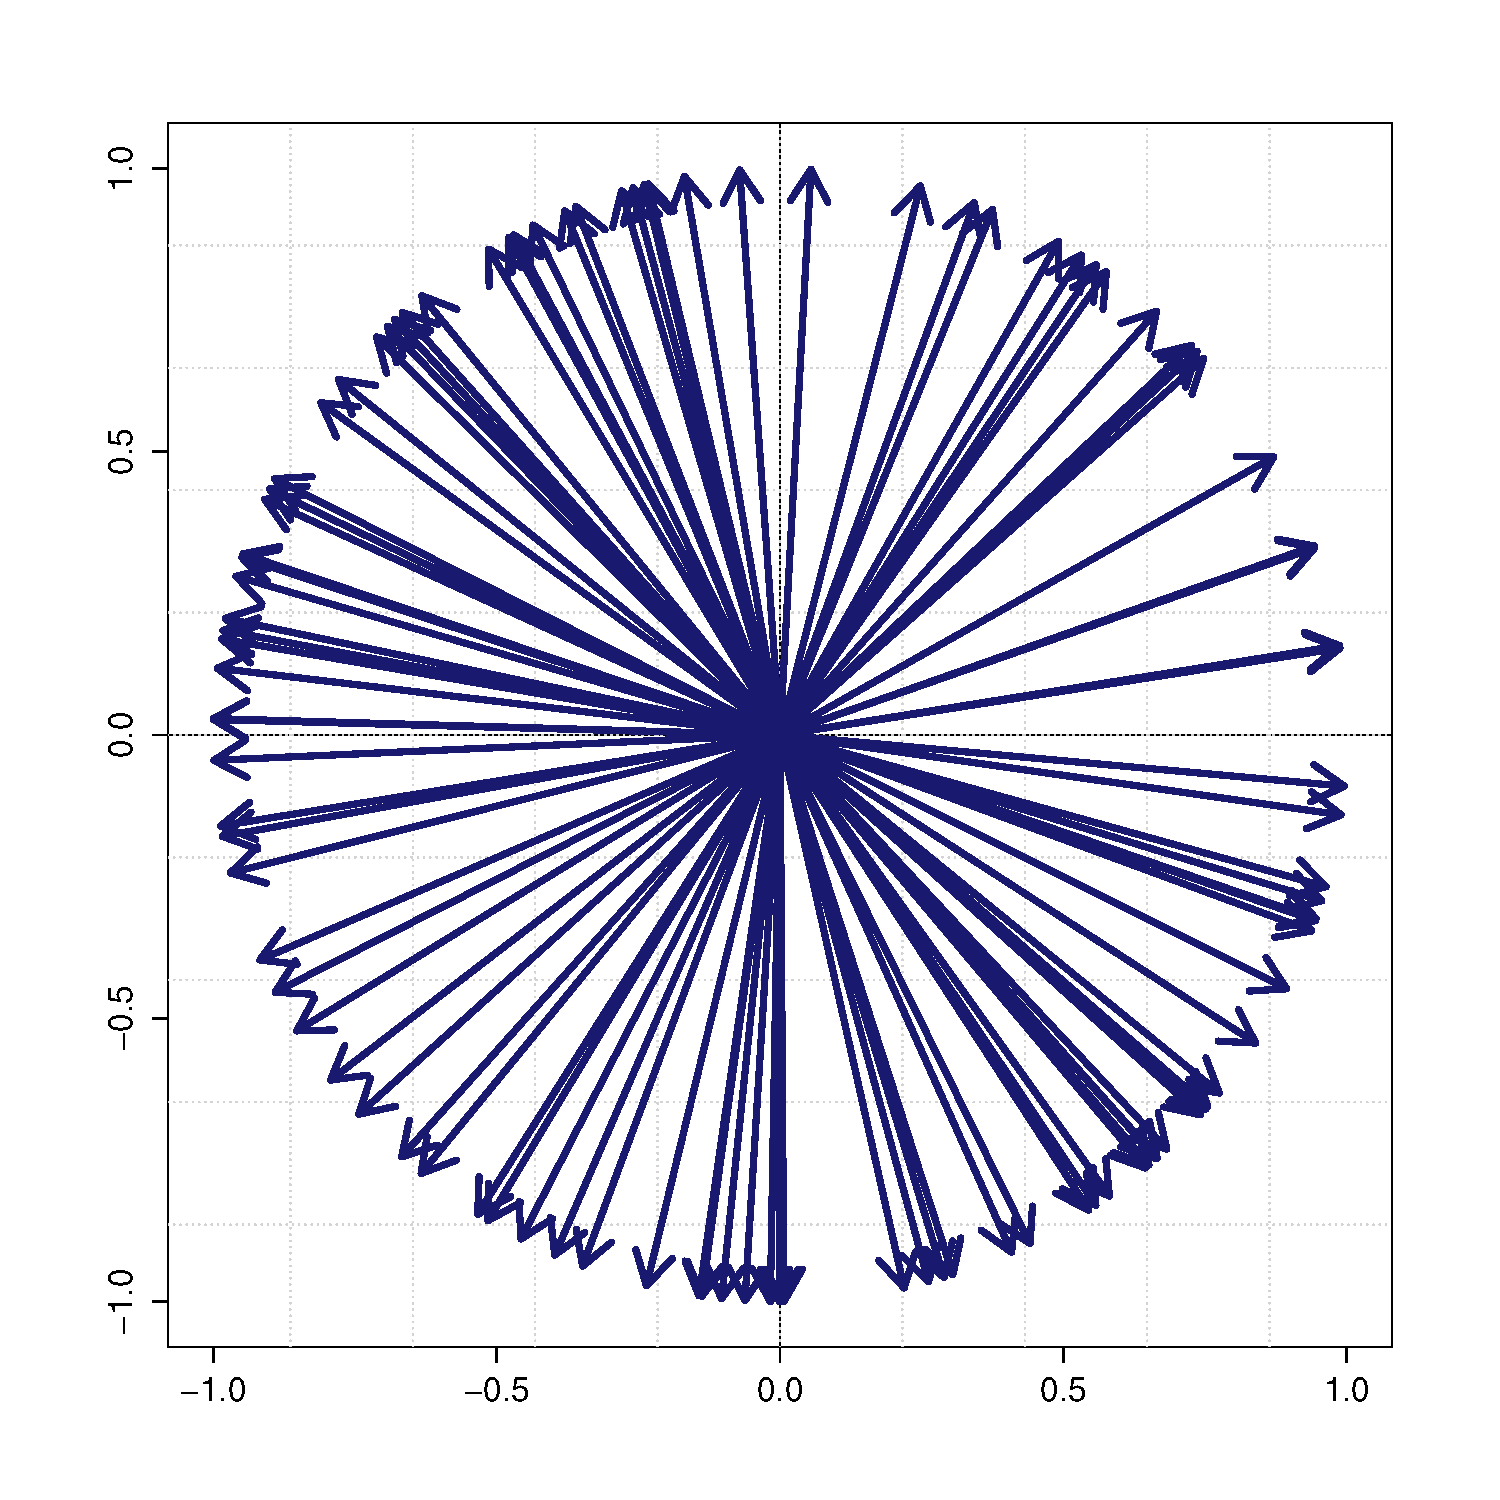
\includegraphics[scale=.3]{./Figures/arbEigen.pdf}%
\figcaption{One-hundred first eigenvectors from samples of size 5000 of a two-dimensional \newline multivariate normal population with $I_2$ covariance structure.}
%\end{minipage}
\end{center}

As a point of comparison we run this same procedure but change the covariance structure. Instead of using a population covariance of $I_2$ we use the $2\times 2$ diagonal matrix $diag(5,3)$. Note how striking the results are. The eigenvalues of $diag(5,3)$ are $\lambda=5,3$ and are thus distinct. The 100 first eigenvectors we plot all sit on top of each other. For a matrix with distinct eigenvalues the eigenvectors are well defined and not so dependent upon the random variations that accompany approximations of $\Sigma$.

%\begin{minipage}{\linewidth}
%\centering
\begin{center}
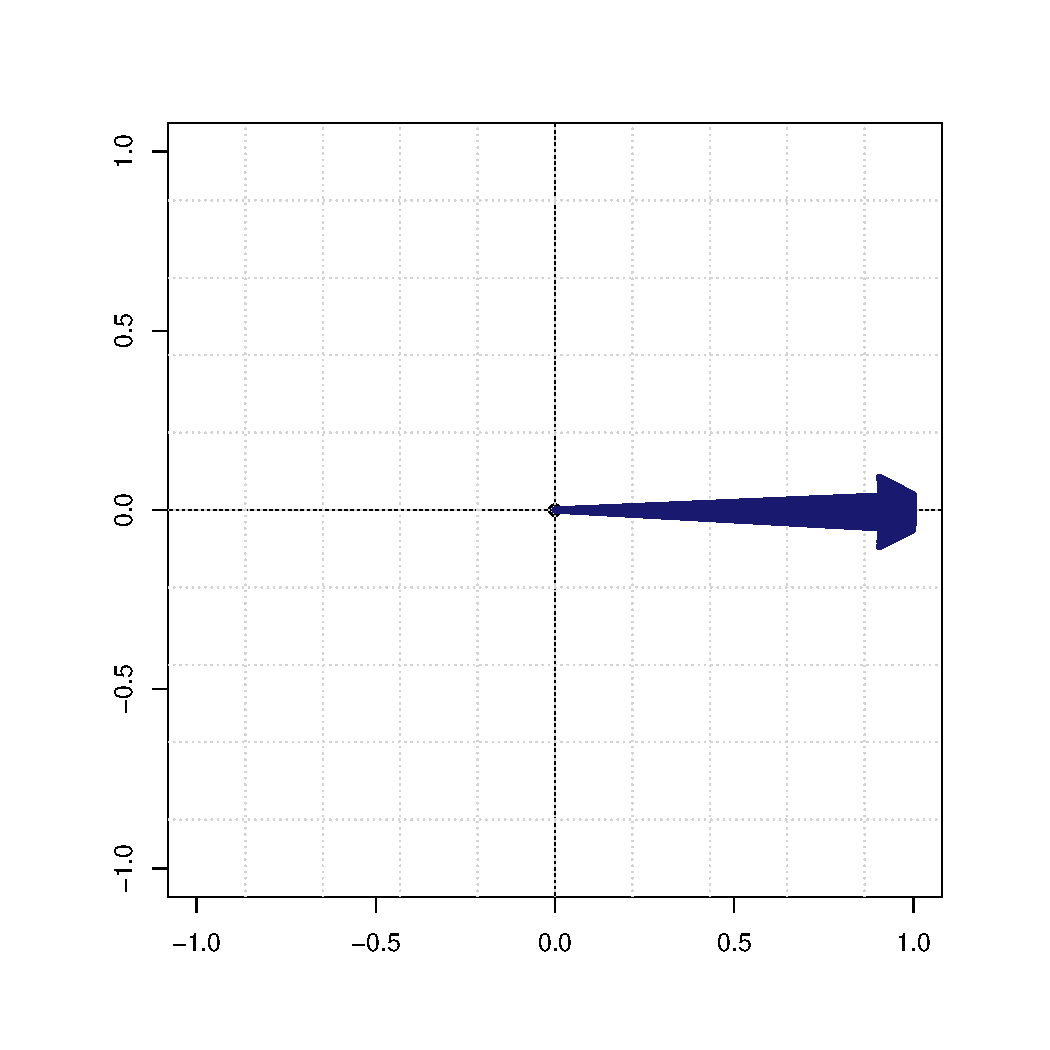
\includegraphics[scale=.3]{./Figures/e2.pdf}%
\figcaption{One-hundred first eigenvectors from samples of size 5000 of a two-dimensional \newline multivariate normal population with $diag(5,3)$ covariance structure.}
%\end{minipage}
\end{center}


Now for covariance structures such as our $I_5$ identity example its not that PCA is giving us the ``wrong'' principal components by using these largely arbitrary eigenvectors. After all \emph{any} orthonormal basis will serve as a correct set of principal components for a truly identity covariance. The problem is that the principal components given to us are completely a product of random error and thus will by no means be constant from one run to the next. They may not even slightly resemble those from a previous run. Furthermore these principal components will not be simple as $PC_i=col(i,X)$. Rather, they will be some horrible, uninterpretable linear combination. This happens despite the fact that the original set of variables defined by the columns of $X$ would describe the data about as well as the more complicated principal components. 


Consider again our starting example with $\Sigma=I_5$ so that the covariance structure underlying the population is an identity matrix. Thus we know that underlying the population there is a very nice set of principal components such that $PC_i=col(i,X)$. However when we take even a large sample, here we use $n=5000$, then we get a set of principal components that are wildly different and wildly more complicated than simply $PC_i=col(i,X)$. Yet clearly we would rather use $PC_1=col(1,X)$ than
$$
PC_1=0.40\,col(1,X)-0.34\,col(2,X)+0.28\,col(3,X)+0.61\,col(4,X)+0.53\,col(5,X).
$$

\subsection{Leverage Scores}

Now clearly the eigenvectors of the sample covariance matrix are fundamental to principal components analysis. However these vectors are also fundamental to the working of CUR. We know that the variables CUR selects are closely related to the leverage scores CUR computes for each column (variable). These leverage scores are, more or less up to a scaling, the probabilities with which CUR keeps each column. As previously discussed, the leverage scores are nothing more than the normalized sum of the squares of the components of the eigenvectors of the sample covariance matrix. 

Consider our example with $I_5$ as the population covariance matrix. We have just discussed at length how the eigenvectors of the sample covariance matrix are going to be random. Now the leverage scores for the columns are calculated using these eigenvectors. Thus it seems a reasonable supposition that the leverage scores are going to be random as well. 

In the following figure we have run the CUR algorithm on 10 different samples from our multivariate normal population with $I_5$ covariance matrix. Each sample has $n=5000$ observations and was mean-centered such that the sample means of the variables are zero. Since the rank of our data is 5 we have calculated the leverage scores for each data set with every possible rank parameter, $k=1,2,\ldots,5$. The color of the dot corresponds to a specific column of the data matrix. The correspondence is the following:

\begin{center}
\begin{tabular}{|c|c|}
 \hline& \\
column number& color\\\hline
1& red\\
2& blue\\
3& green\\
4& orange\\
5& black\\
\hline
\end{tabular} 
\end{center}

Looking at the figure our hypothesis is largely justified. There is not a discernible pattern to the leverage scores. One column (color) does not appear to generally have a higher leverage score than the others. Similarly there don't seem to be any columns that are generally lower than the others. This is precisely how we would expect randomly generated leverage score to present themselves. The only noticeable feature of the graphs is that the leverage scores converge to $.2=\frac{1}{5}$ as $k$ increases. However this convergence true of any leverage scores from any data. If $S$ is our sample covariance matrix then the leverage scores will always converge to $1/rank(S)$ as $k\rightarrow rank(S)$. 

So it seems that for this very simple data with an underlying covariance matrix of $I_5$ the leverage scores are meaningless. They will not help us distinguish among columns as they are random. However I think it would be unfair to say that CUR does poorly on this data as a result. The identity covariance structure ensures that all of the columns are, in a large sense, the same. So it doesn't much matter which columns we choose. Any column is as good as any other. Nonetheless we should generally be cautious to interpret the leverage scores as capturing importance. This very simple data is an example where these scores in no way capture any importance. \newpage

%\newpage
%\begin{minipage}{\linewidth}
%\centering
\begin{center}
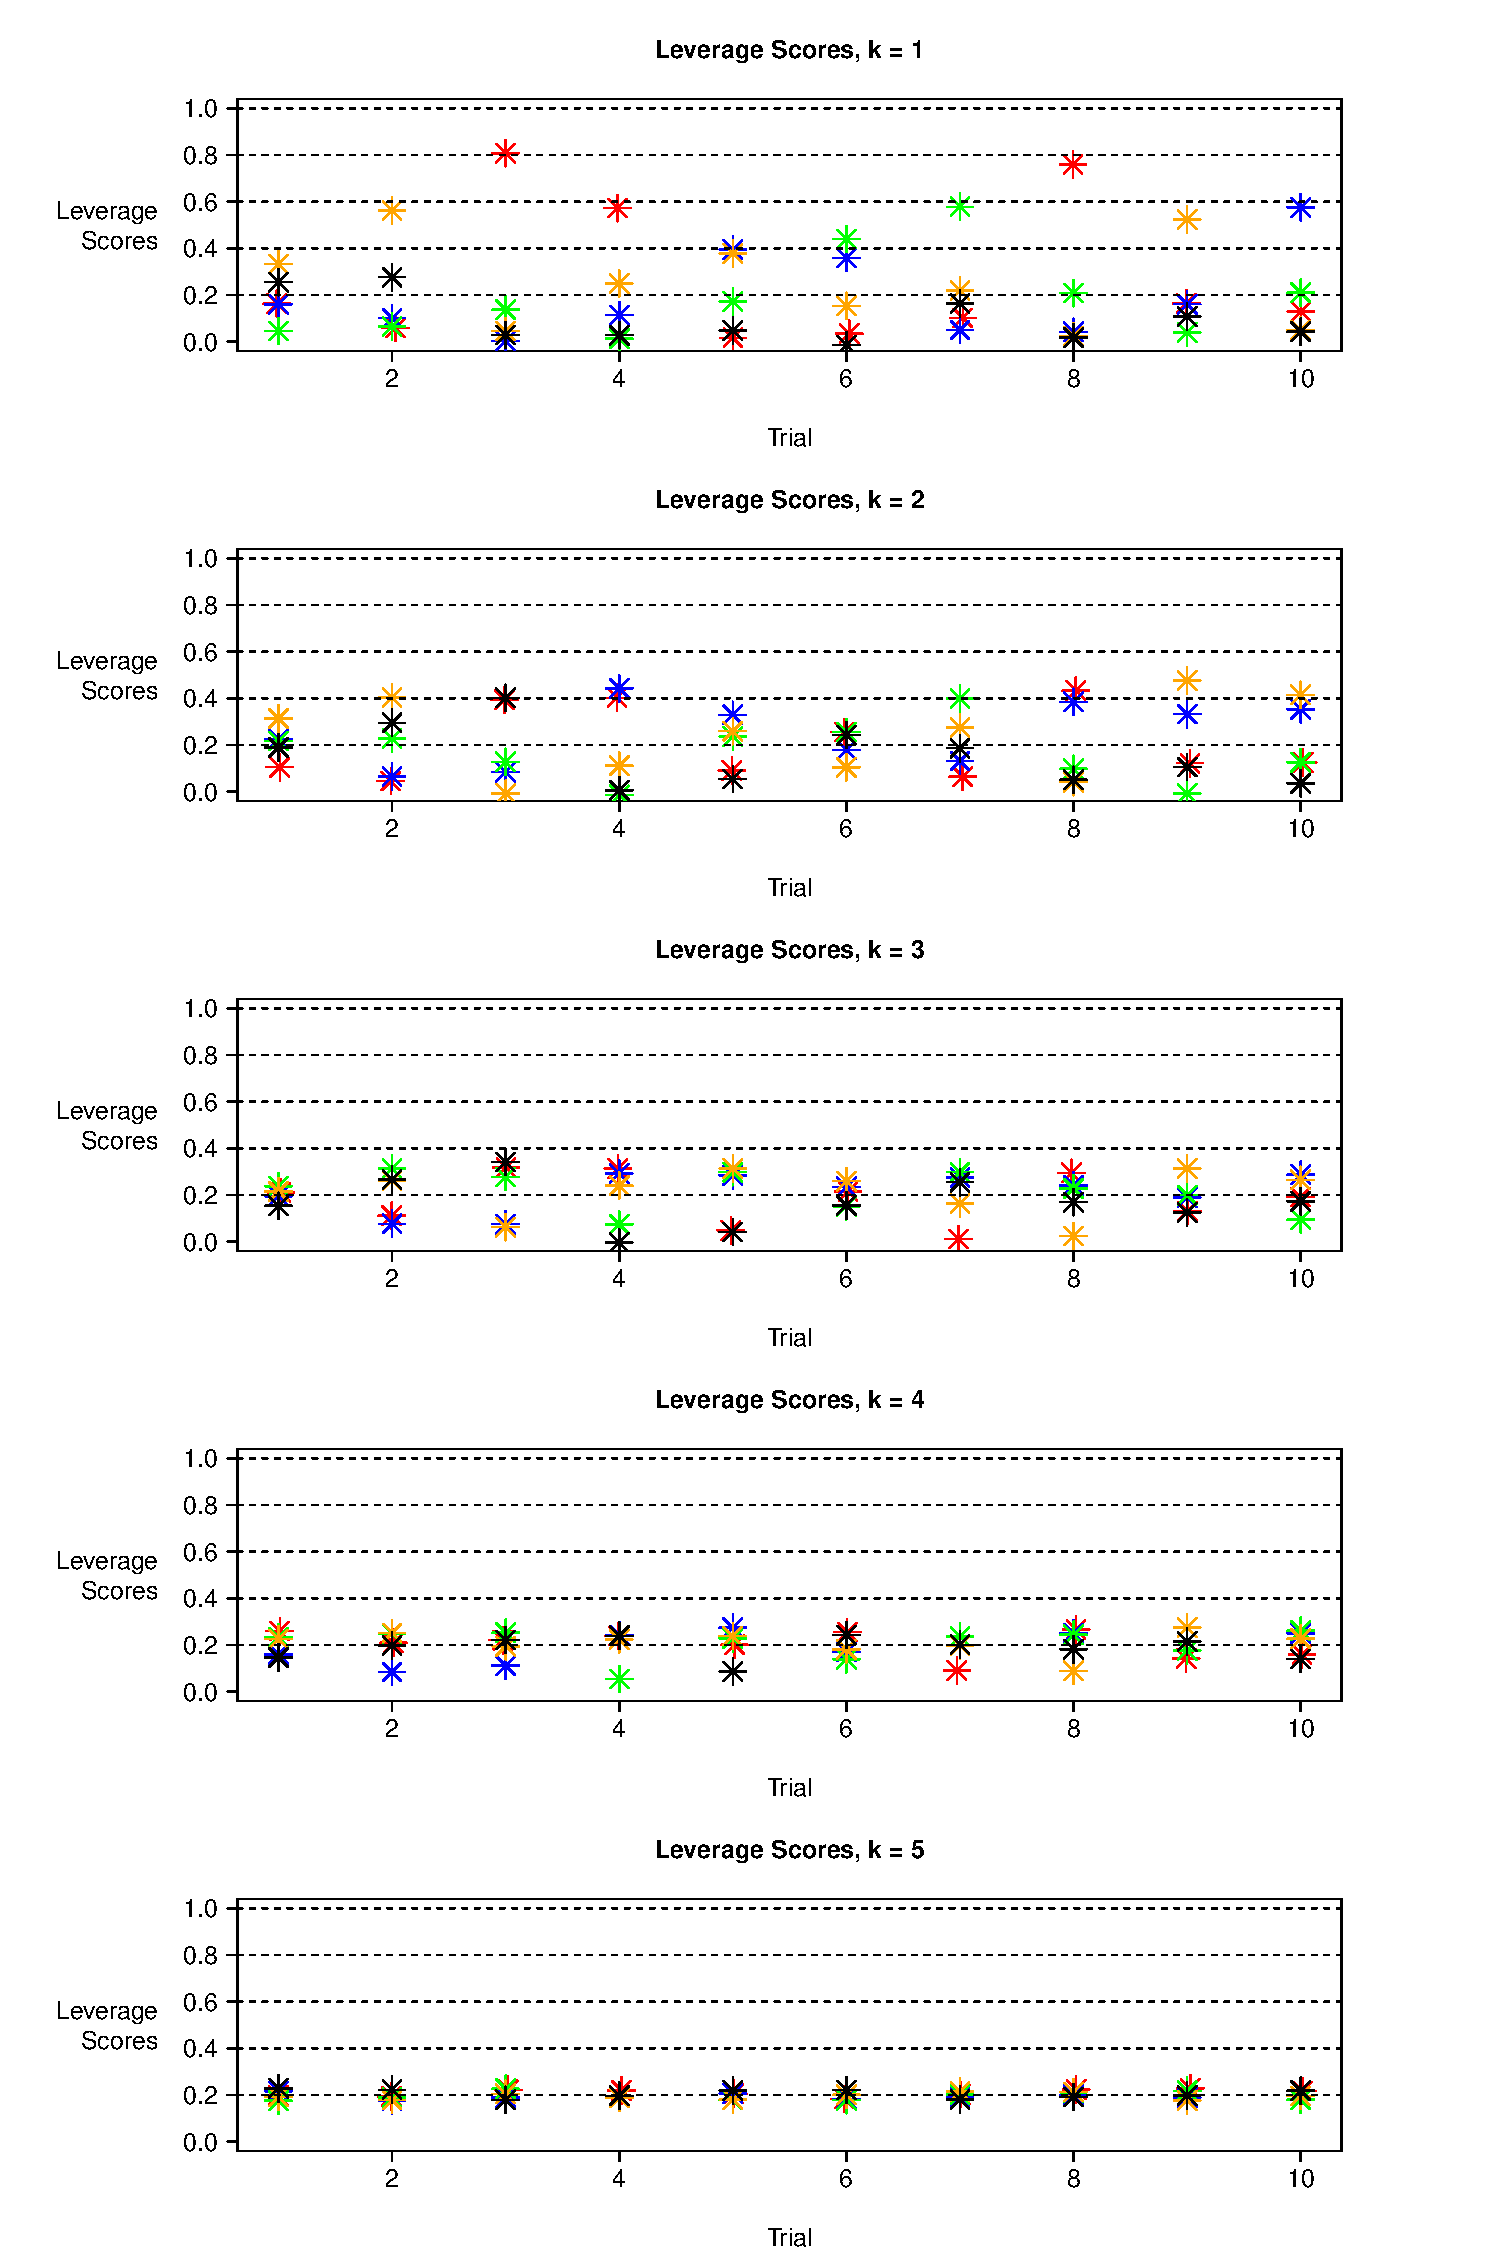
\includegraphics[scale=.60]{./Figures/levs4.pdf}%
\figcaption{The leverage scores of data generated from a multivariate normal $N_5(0,I_5)$ with sample sizes of $n=5000$.}
\end{center}
%\end{minipage}
\pagebreak

\subsection{Columns Chosen}
To confirm some of our suspicions about the performance of CUR on this data let us explore this example further. Now we know that CUR has a column parameter $c$ which approximately controls for how many columns we choose. We discussed the precise workings of this parameter is Chapter 3. Let us look at what this parameter does empirically. 

In Figure $4.4$ we have made for each value of the rank parameter $k=1,\ldots,5$ a plot of the average number of columns chosen by CUR (over $N=1000$ runs) for each value of the column parameter $c=0,\ldots,5$. That is, for each rank and column parameter pair $(c,k)$ we have run CUR on our data matrix 1000 times and recorded the average number of columns chosen. While in the literature we can't have $c=0$ we include this in our analysis for completeness. We think of $c=0$ as a run where CUR chooses no columns. This may seem strange because we know that CUR must choose at least one column. The convention to include this will hopefully make sense shortly. 

The blue line in each plot is a line with slope $1$. If a point in our plot is on this line then the average number of columns chosen is equal to the column parameter $c$. We can see from the plots that our points follow the blue line closely. That is, the average number of columns chosen is always very close to the column parameter $c$ we give the algorithm. Thus as we discussed in the previous chapter we are largely justified in saying that 
$$
\text{E}\left[\mathscr{C}\right]\approx c.
$$
An important point here is that this is true regardless of the value of the rank parameter $k$. At least in our present identity covariance example the rank parameter seems to have negligible impact on the number of columns chosen. The latter always seems to be about $c$. This will simplify our analysis greatly because we can now think of running CUR with a column parameter $c$ as selecting ``about'' $c$ columns. 
\newpage

\begin{center}
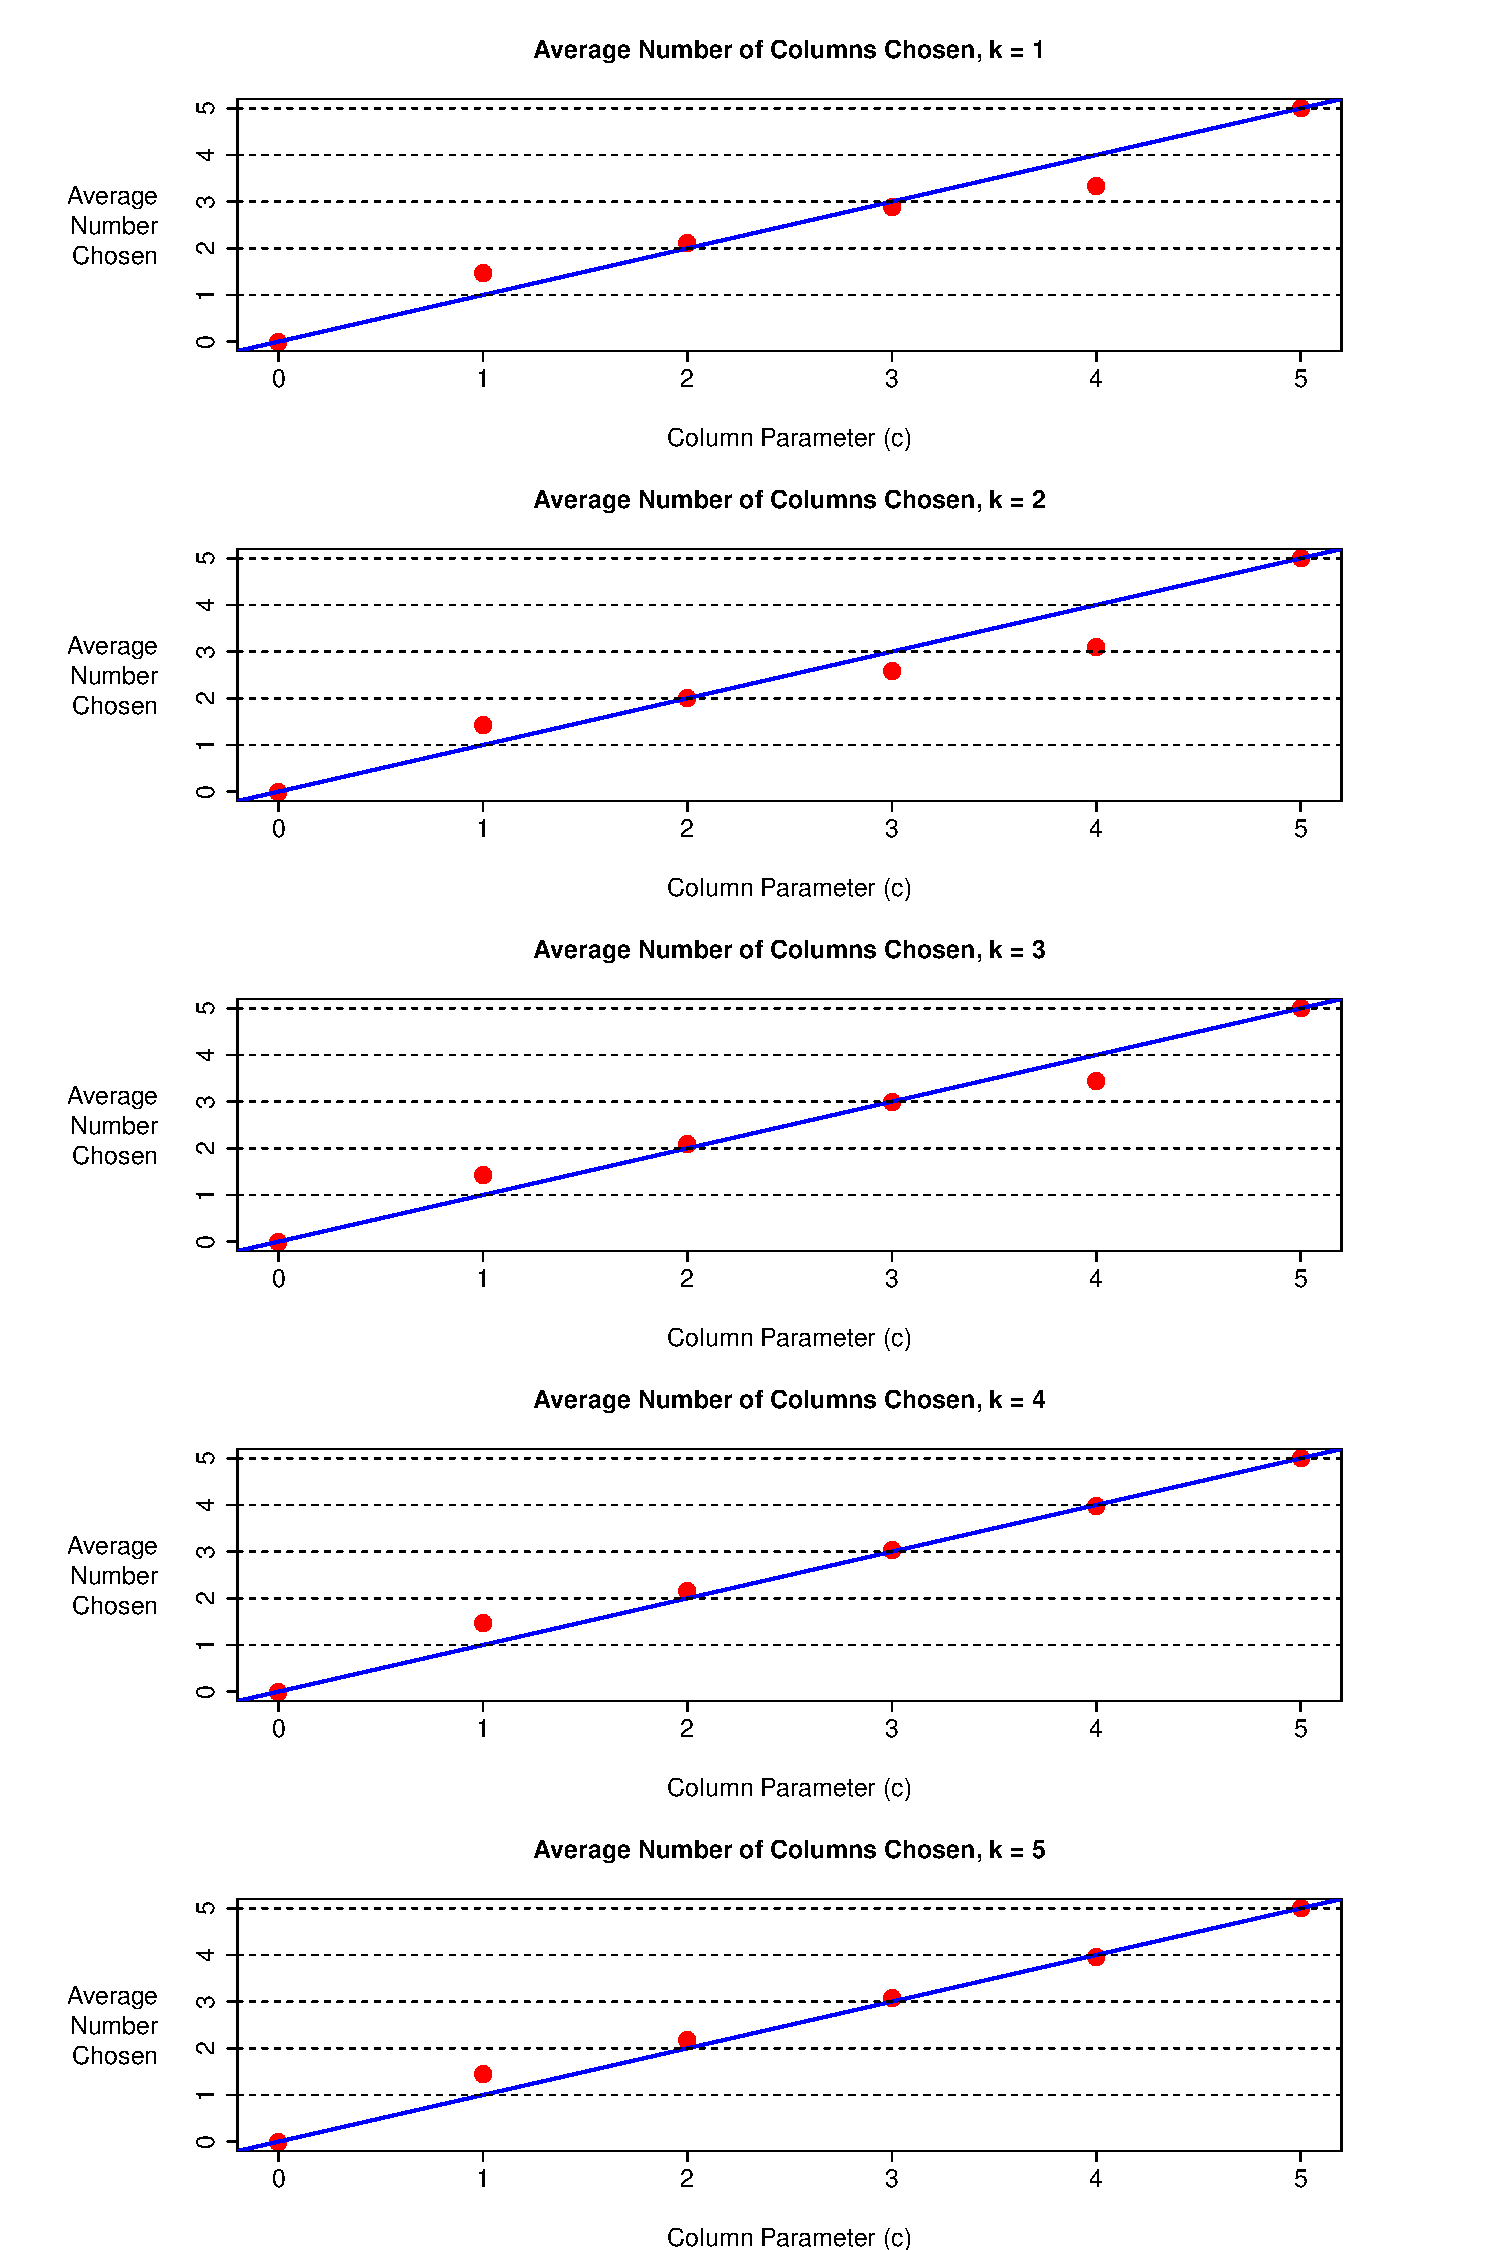
\includegraphics[scale=.59]{./Figures/diag_ex_1_chosen_v_c.pdf}%
\figcaption{The average ($N=1000$) number of columns chosen for every permissible value of the rank and column parameters $c$ and $k$. The blue line has slope $1$. }
\end{center}
\pagebreak


\subsection{Effectiveness}

Now the main goal of this paper is to compare the performance of CUR and PCA. For multivariate normal data a natural way to evaluate the performance of CUR or PCA is to see how much variance is captured by each method. We are using both CUR and PCA to reduce the dimensionality of our data set. In PCA we compute $k$ principal components and make a new data matrix $D$ comprised of these components. In CUR we retain approximately $c$ columns of our matrix and create a new data matrix $C$ whose columns are comprised of the CUR chosen columns. In both of these methods we are throwing away part of our data. The most natural way to measure this loss is by computing how much variance we lose, or equivalently, how much variance we retain. Then to measure the performance of CUR relative to PCA we propose the following statistic. For a data matrix $X$, matrix $D$ comprised of $k$ principal components of $X$ and matrix $C$ comprised of the columns of $X$ chosen by CUR let
$$
e=\frac{||C||^2_F-||D||_F^2}{||X||^2_F}.
$$
be the effectiveness of CUR relative to PCA. Let us now look at what this statistic means. 

Remember that for a centered data matrix $X$ the total sample variance of $X$ is $\frac{1}{n-1}||X||^2_F$. Thus $\frac{1}{n-1}||X||^2_F$ is the total variance originally in the unaltered data, $\frac{1}{n-1}||D||^2_F$ is the total variance retained by using PCA and $\frac{1}{n-1}||C||^2_F$ is the total variance retained using CUR. Then
$$
e=\frac{\frac{1}{n-1}||C||^2_F-\frac{1}{n-1}||D||_F^2}{\frac{1}{n-1}||X||^2_F}.
$$
and is thus the total variance retained by CUR less the total variance retained by PCA normalized by the total variance in the original data set. 

Now if $e > 0$ then $||C||_F^2>||D||_F^2$ and so CUR retains more of the variance than PCA. Similarly if $e<0$ then $||C||_F^2<||D||_F^2$ and so CUR retains less of the variance than PCA. The difference
$$
d=||C||_F^2-||D||_F^2
$$
is the amount of variance CUR retains over PCA. If $d<0$ we interpret this as meaning that PCA retains $|d|$ variance over CUR. In calculating $e$ we normalize this $d$ by by $||X||_F^2$ getting $e=d/||X||_F^2$. Thus we can interpret $e$ as the percentage of the total variance of the data set that CUR retains over PCA. 

Finally note that
$$
-1< e < 1.
$$
because neither CUR nor PCA can do better than retaining $100\%$ more variance than the other. 


For our data matrix $X$ we make a plot of the average effectiveness value $e$ over all possible values of $c$ and $k$. That is, for every value $0\leq c \leq p=5$ and $1 \leq k \leq rank(X)=5$ we plot the average effectiveness value $e$ running CUR with rank parameter $k$ and column parameter $c$ and retaining $k$ principal components when conducting PCA. 

Note that in general the rank parameter given to CUR and the number of principal components retained by PCA need not be the same. However for our purposes when comparing CUR to PCA we will always set them equal to some common value $k$. Remember that the rank parameter $k$ in the CUR algorithm controls how the leverage scores are generated. A rank parameter of $k$ means that the leverage scores for the columns of the matrix are computed using the first $k$ principal components of the matrix. For a rank parameter of $k$ the leverage score $\ell_i$ captures, in some sense, the ``like-ness'' of the $i^{th}$ column to the first $k$ principal components. We want to use CUR to do something similar to PCA. Thus if we are going to retain $k$ principal components in our analysis we should use CUR to find columns of our data matrix that do something similar to the first $k$ principal components we retain. Thus we should set the rank parameter of the CUR algorithm to the same $k$ controlling how many principal components we retain. 

\begin{center}
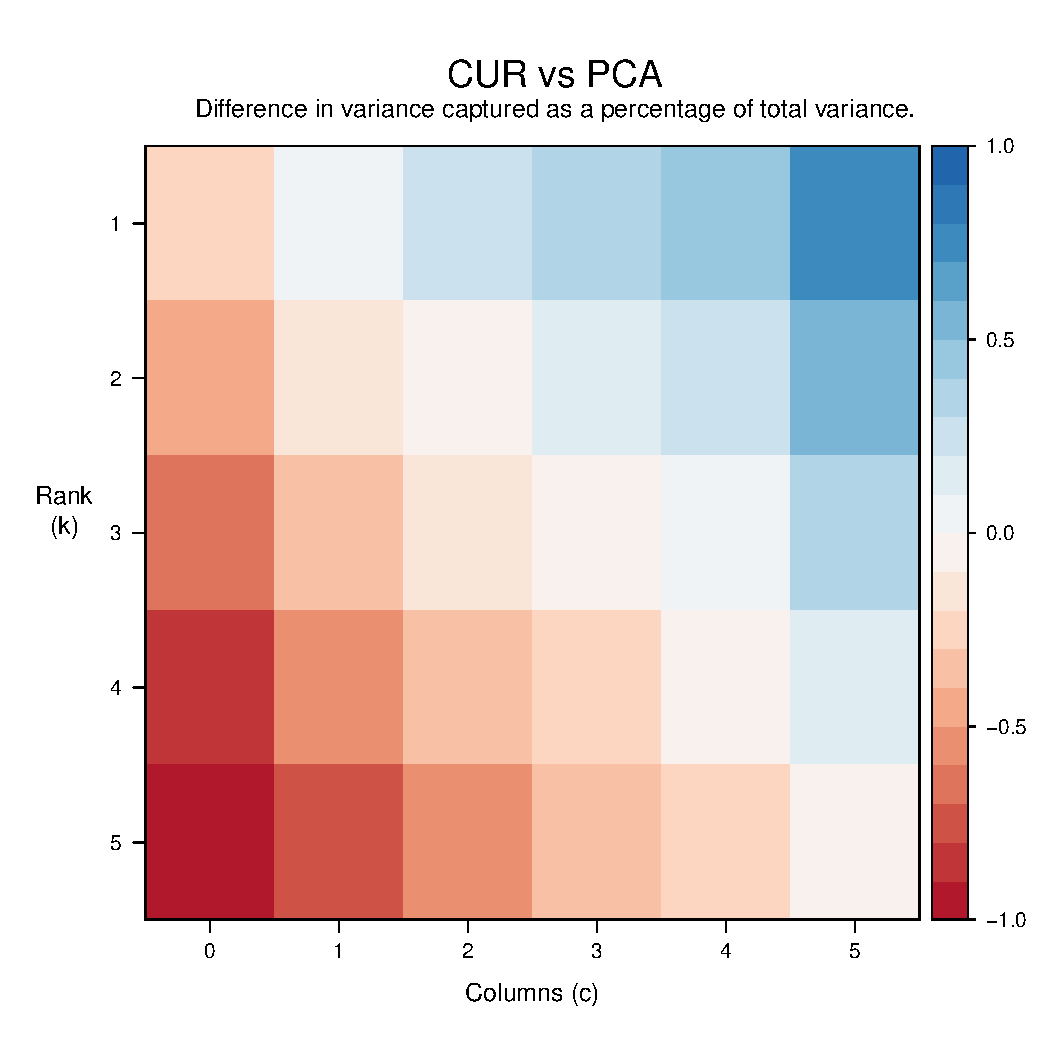
\includegraphics[scale=.75]{./Figures/diag_ex_1_raster.pdf}%
\figcaption{A plot of the average ($N=1000$) effectiveness value $e$ for each possible value of the rank and column parameters $c$ and $k$.}
\end{center}

The color in each box of the plot (as indicated by the key) corresponds to the effectiveness score. The more blue the color the closer the effectiveness score is to $1$ and thus the better CUR performs in comparison to PCA. The darker red the color the closer the effectiveness score is to $-1$ and thus the better PCA performs in comparison to CUR. The closer the box is to being white the closer $e$ is to being zero in which case there is no noticeable difference between CUR and PCA as measured by our effectiveness metric. 

Note again that we run our calculations for $e$ having the column parameter $c$ range from zero to five, the number of columns of $X$. While we can't actually run CUR with $c=0$ the values in this first column of our plot correspond to the amount of variance captured by PCA over all the values of $k=1,\ldots,rank(X)=5$. In the case that $c=0$ we are pretending the $C$ matrix is the zero matrix (of any size) so that the calculation for the effectiveness score $e$ becomes
$$
e=-\frac{||D||_F^2}{||X||_F^2}.
$$
For any $k$ the absolute value of this quantity is simply the percentage of variance retained by running PCA and keeping $k$ principal components. 

As we move down the first column of our plot (i.e. we keep $c=0$ and increase $k$) we notice that as $k$ increases the boxes become darker red. This makes sense because as we increase $k$ we are increasing the number of principal components retained by PCA and thus the percentage of variance captured by PCA. The last box where $c=0$ and $k=5$ has a effectiveness score of $e=-1$ since we are retaining all of the principal components and thus capturing $100\%$ of the variance. This first column of the plot should be seen as a reference column of how PCA performs by itself on the data for the various values of $k$. 

Now the most striking feature of this plot is seen if we look at the boxes in relation to the line $c=k$. Notice that boxes corresponding to $(c,k)$ pairs of $(1,1),(2,2),\ldots,(5,5)$ are all white. That is, the effectiveness score is zero and so there is relatively little difference between the performance of CUR and PCA on the data. Now the boxes below this line of $c=k$ are all red meaning that PCA does relatively better than CUR. Similarly the boxes above the line are all blue meaning that CUR does relatively better than PCA. Furthermore the intensity of each color increases the further we move from the line $c=k$. This is an explainable pattern. 

Firstly remember that the covariance matrix for this data is essentially an identity matrix. Thus there isn't really reason to prefer one column above any other. All the columns capture about the same amount of variance. Secondly remember having a column parameter of $c$ in the CUR algorithm means we will retain about $c$ columns of the data matrix. Note that this was true regardless of the rank parameter $k$. Look back to Figure 4.4 to remember this. What this means is that the amount of variance captured by CUR is purely a linear function of \emph{how many} columns CUR chooses. 

To see this consider the following two plots. Figure 4.6 is similar to Figure 4.5. However in Figure 4.6 we plot only the variance captured by CUR. In Figure 4.6 the color in each box corresponds to the value of 
$$
\frac{||C||_F^2}{||X||_F^2}.
$$
This value is the percentage of total variance of $X$ captured by the CUR algorithm. It is simply the first half of the calculation for the effectiveness score
$$
e=\frac{||C||_F^2}{||X||_F^2}-\frac{||D||_F^2}{||X||_F^2}.
$$
We can see in Figure 4.6 that the percentage of the total variance captured by CUR changes only as a function of the column parameter $c$. The percentage of variance captured is essentially constant down each column. Thus the rank paramter doesn't seem to affect the percentage of variance captured by CUR. Figure 4.7 shows us that the relationship is essentially a linear function of the column parameter $c$. Figure 4.7 just plots the average values of the columns of the plot in Figure 4.6. 

\begin{center}
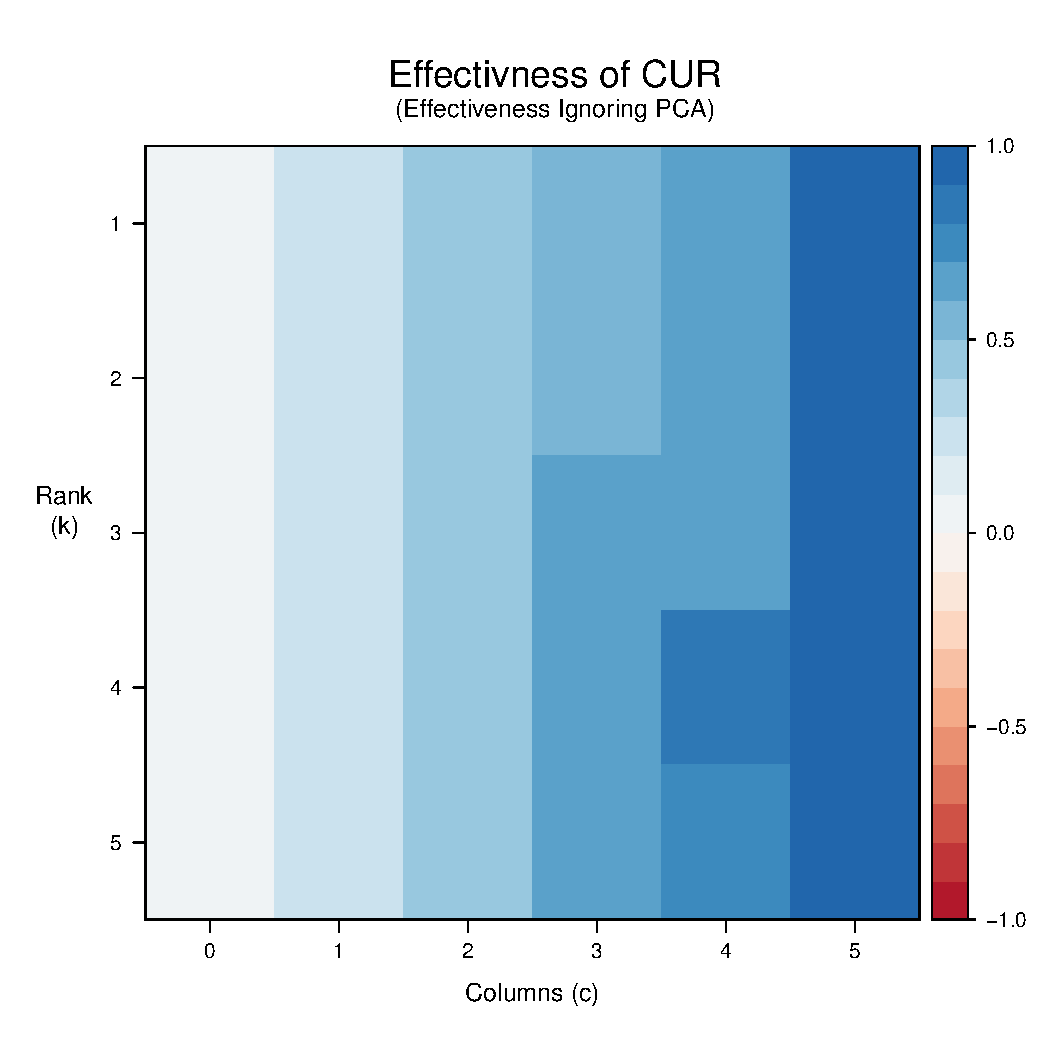
\includegraphics[scale=.63]{./Figures/diag_ex_1_cur_raster.pdf}%
\figcaption{A plot of the average percentage of variance captured by the CUR algorithm ($N=1000$) for each possible value of the rank and column parameters $c$ and $k$.}
\end{center}


\begin{center}
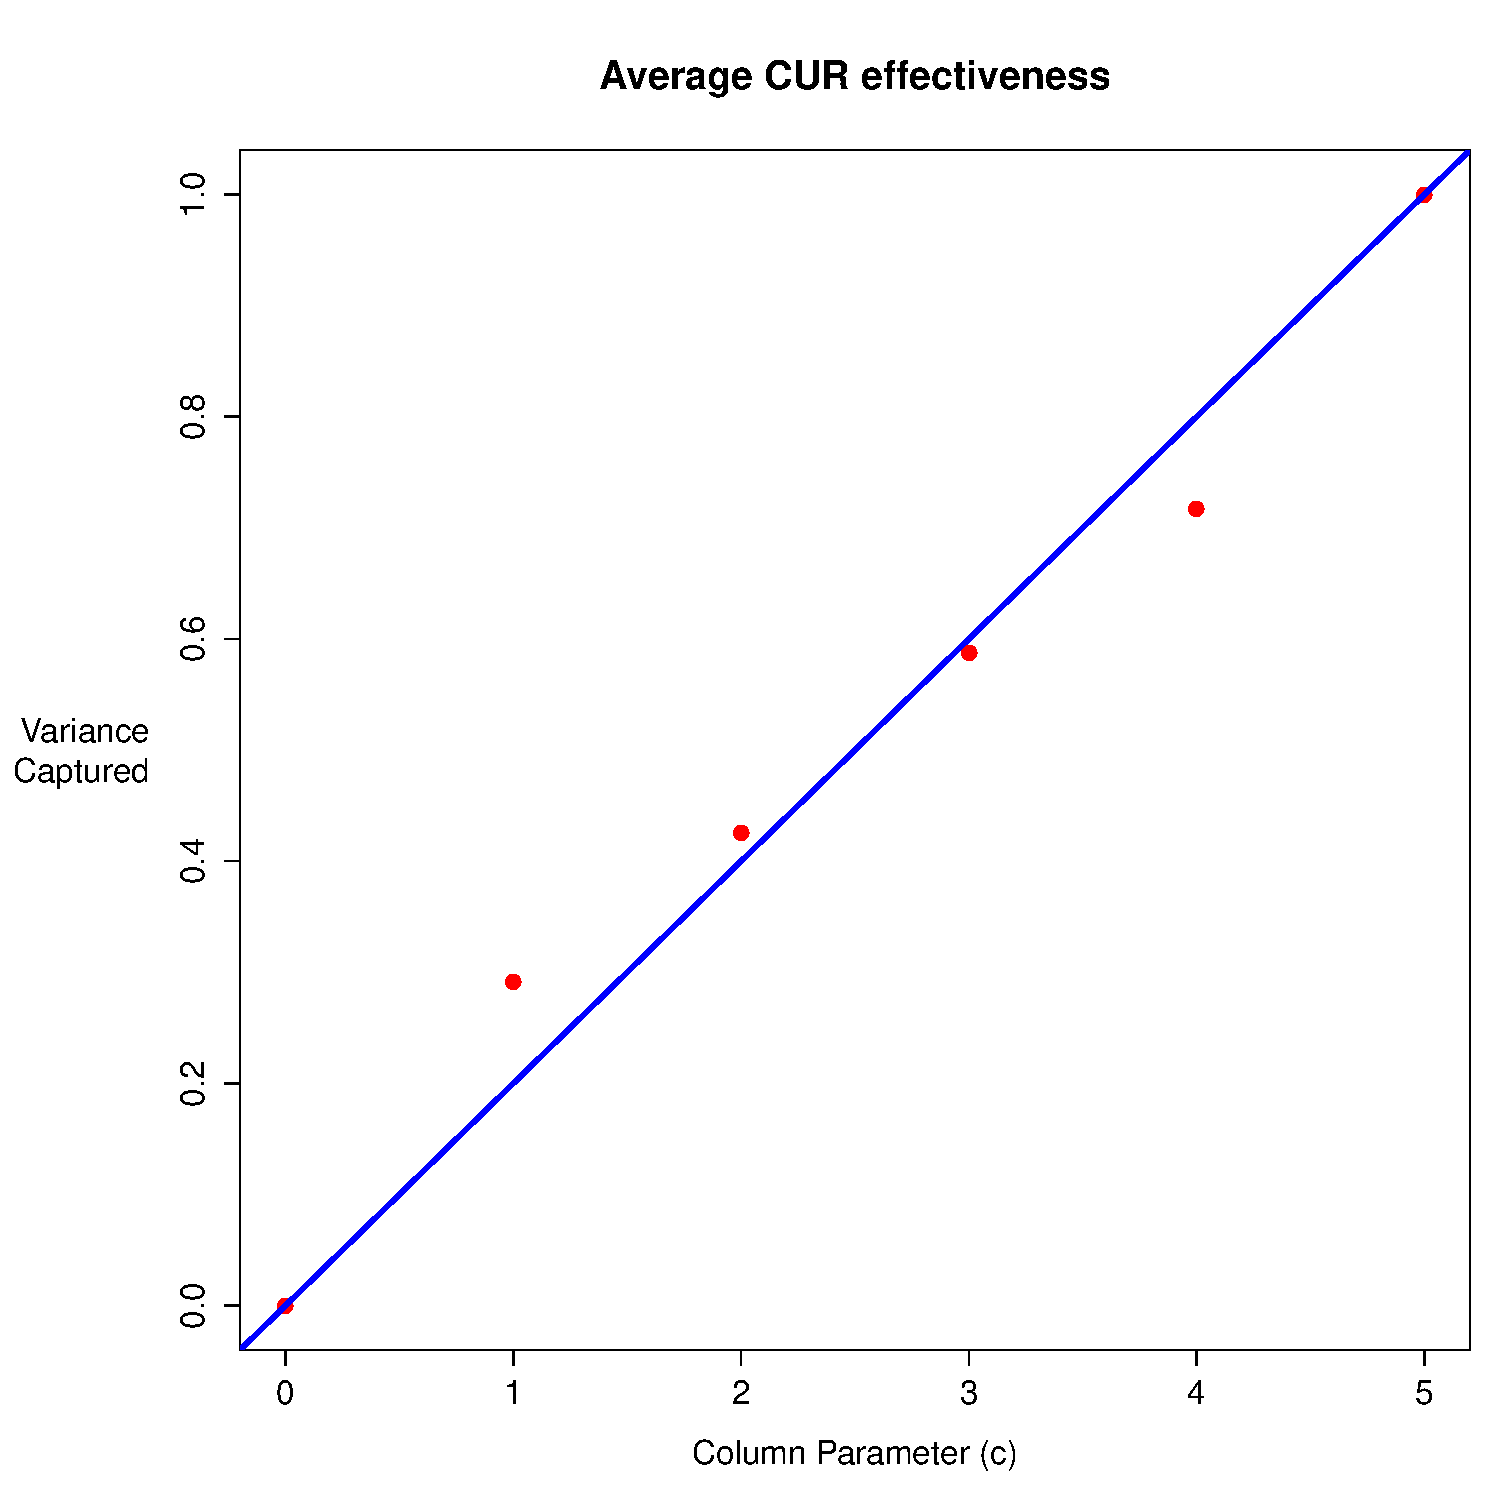
\includegraphics[scale=.43]{./Figures/diag_ex_1_cur_effect_avg.pdf}%
\figcaption{A plot of the average percentage of variance captured by the CUR algorithm ($N=1000$) averaged across the different rank parameter ($k$) values. The blue line has a slope of $1/5$.}
\end{center}

However the variance captured by CUR is only half of the effectiveness calculation. We haven't included any of the information regarding how PCA behaves. Thus we do something similar for PCA. The plot in Figure 4.8 is the plot of the average percentage of variance captured by PCA for every value of the rank and column parameters $c$ and $k$. Note that since PCA is not a function of the column parameter $c$ then the amount of variance captured is constant across the rows. Indeed the graph is what we get if we simply repeat the first column of Figure 4.5 for every column. The colors in this plot correspond to the value of
$$
-\frac{||D||_F^2}{||X||_F^2}
$$
which is the second half of the effectiveness score.  

Similarly the plot in Figure 4.9 is the corresponding average across the rows of the variance captured in Figure 4.8. This is the corresponding graph to Figure 4.7. Note that the points on this graph are almost perfectly linear. 


\newpage 
\begin{center}
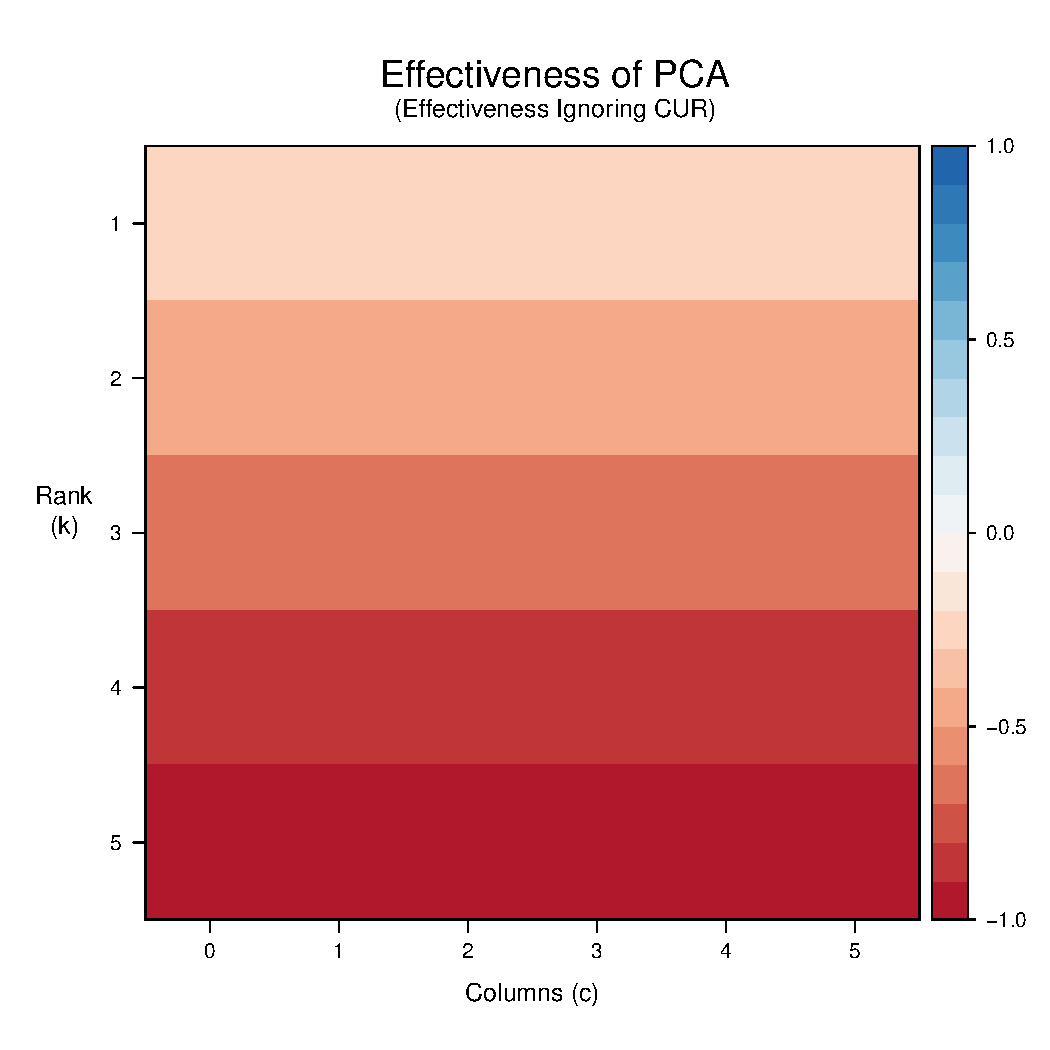
\includegraphics[scale=.63]{./Figures/diag_ex_1_pca_raster.pdf}%
\figcaption{A plot of the average percentage of variance captured by PCA ($N=1000$) for each possible value of the rank and column parameters $c$ and $k$.}
\end{center}


\begin{center}
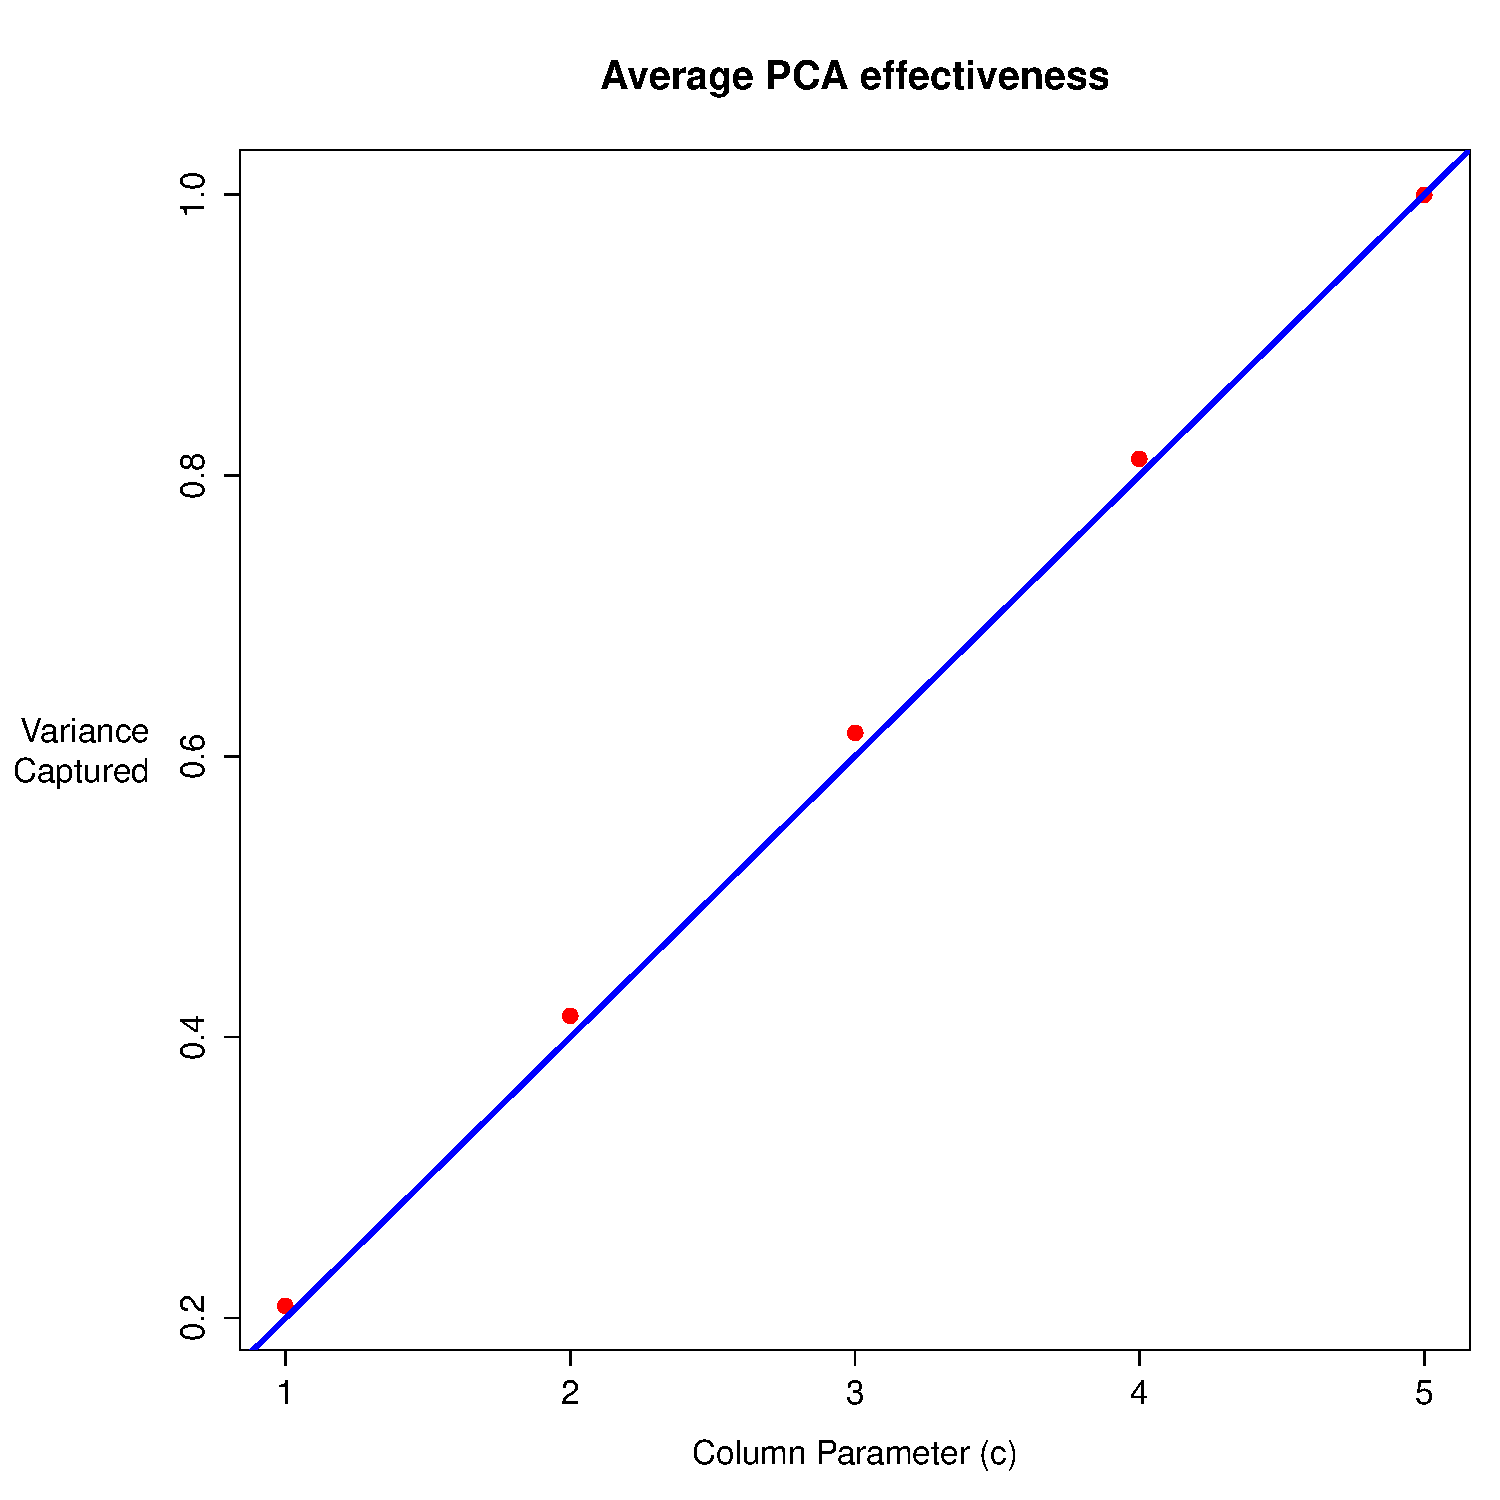
\includegraphics[scale=.43]{./Figures/diag_ex_1_pca_effect_avg.pdf}%
\figcaption{A plot of the average percentage of variance captured by PCA ($N=1000$) averaged across the different column parameter values. The blue line has a slope of $1/5$.}
\end{center}
\pagebreak 

Now the plot in Figure 4.5 is simply the superposition of the plots in Figure 4.6 and 4.8. In figure 4.6 we see that CUR does better linearly as the column parameter increases. In figure 4.8 we see that CUR does better linearly as the rank parameter increases. The combination of these two behaviors produces the pattern we see in Figure 4.5. CUR does relatively better than PCA only when $c>k$ and PCA does relatively better than CUR when $c<k$. Note that they both do about the same when $c=k$. 

Thus, at least in terms of the effectiveness score $e$, CUR does as well as PCA for $c \geq k$. Note however that this effectiveness score only tells us about the difference in variance captured between the two methods. Our goal with CUR is not purely one of capturing variance.  At least half of our goal in using CUR is to reduce the dimensionality of our data while maintaining interpretability of the variables. Now generally the selected variables by CUR will be more interpretable than the linear combinations of these variables produced by PCA. Thus running CUR ``in the blue'' where $c \geq k$ and the variance captured by CUR using these values of $c$ and $k$ is at least that captured by PCA seems a reasonable thing to do. When doing this we will get a more interpretable selection of variables and capture at least as much of the data's variance as we would have using PCA. Note however that one could extend this line of thought and possibly argue that CUR would still be effective slightly below the line $c=k$. In Figure 4.5 we see that in this region PCA does slightly better than CUR. That is, we capture a little less variance using CUR than running PCA. However if we gain interpretability from running CUR then we might be willing to trade some fidelity in our description of the data (variance captured) for ease of interpretation. Thus one could argue that CUR is still effective on this data when $c$ is slightly smaller than $k$. 

Now it should be noted that since $k$ determines the number of principal components retained by PCA then $k$ determines the dimension of the reduced data produced by PCA. Furthermore since $c$ approximately determines the number of columns chosen by CUR then $c$ approximately determines the dimension of the reduced data produced by CUR. Thus any effective use of CUR can't have the column parameter $c$ be too large. CUR will do relatively well in terms of variance captured if we let $c=p$, the number of variables. However if we are retaining all of the variables of the data then we aren't meeting our goal of dimensionality reduction with CUR. Thus generally we want to have a $c$ (much) smaller than the rank of our data matrix since it is only in this case that we are actually reducing the dimensionality of our data. 

Thus in our above example what really makes CUR effective on this data is the fact that we have a non-negative value for $e$ for relatively small values of $c$. Using this data we see that the effectiveness score $e$ is approximately zero when $c=k$. Thus instead of running PCA and retaining $c=k$ principal components we can run CUR and retain about $c=k$ actual columns of our data matrix. We don't do any worse in terms of the amount of variance we captured however we will do much better in terms of interpretability. Remember that the principal components for this data were horrible linear combinations of the columns of $X$ whereas the CUR chosen variables are simply individual columns. 

\subsection{Conclusion}

There are several features of this analysis which we expect to see in future analyses. Similarly there are features of this data which make its analysis unique. These features will likely become evident as we continue in this paper. However it seems worthwhile to point them out now so that one is aware at the outset. 

Note in Figure 4.5 PCA does better than CUR for $c<k$. This is generally going to be a feature of the effectiveness score $e$ so long as the number of columns chosen by CUR tracks with the column parameter $c$. It is a mathematical theorem that the $k$ principal components are the linear combinations of our columns that capture the most variance among all such sets of $k$ linear combinations of the variables. A corollary is that we are never going to capture more variance than these first $k$ principal components using $m<k$ linear combinations of the variables. Since we may view the columns of the matrix $X$ as very simple linear combinations of the columns of $X$ then if we choose $c<k$ columns we can never capture as much variance with these $c$ columns as with the $k$ principal components. Hence the effectiveness score will always be negative because $||D||^2_F>||C||_F^2$. This statement isn't perfectly precise because the column parameter $c$ only controls the expectation of the number of columns to be chosen. Thus on any given run it is possible that $c<k$ and yet we choose more than $k$ columns. However on average, as seen in Figure 4.5, when $c<k$ then $e<0$. 

Now we previously noted that we didn't want our column parameter $c$ to be too far above $k$. Furthermore as we just discussed we also don't want $c$ to be too far below $k$ since they we will be giving up too much variance. Thus it seems that the Goldilocks region for our $c$ parameter is when $c \approx k$. Now in this example it happened that in this region where $c\approx k$ we had that $e \approx 0$ and so CUR would perform about as well as PCA and thus the CUR algorithm could be reasonably effective in this region. However this will not always be true. This was a product of the fact that PCA did better linearly as $k$ increased and CUR did better linearly as $c$ increased. This was very much a product of the underlying covariance structure $\Sigma=I_5$. As we will see for arbitrary covariance structures there is not always such a simple relationship between the variance captured by PCA and CUR and the $k$ and $c$ parameters respectively. Hence there is not always such a simple pattern for the effectiveness of CUR as seen in Figure 4.5. In this light two very important questions in our future analyses will be (1) how does this effectiveness score $e$ behave when $c \approx k$ and (2) how far from the line $c=k$ do we need to get before we have a non-negative $e$ value. 



\newpage 
\section{Example 2: Diagonal with Distinct Eigenvalues}

Now the behavior of the last example was heavily influenced by the fact that the eigenvalues of the covariance matrix were all equal. Let us look at the other extreme and consider what happens when we have a diagonal covariance matrix with all distinct eigenvalues. 

\subsection{The Data}


As previously consider $\rv{X}$ to be a multivariate normally distributed random vector containing $p=5$ component random variables. Furthermore let the covariance matrix $\Sigma$ of $\rv{X}$ be the diagonal matrix $\Sigma=diag(5,4,3,2,1)$. Thus the entries down the main diagonal decrease linearly. As previously the population mean is inconsequential. In this example we take a sample of $\rv{X}$ and construct a (centered) $n\times p$ data matrix $X$ consisting of $n=5000$ samples of $\rv{X}$. For comparison's sake we have kept all the parameters of the $\rv{X}$--distribution constant from Example 1 except the underlying covariance matrix $\Sigma$. Now instead of $\Sigma$ being $I_5$ it is $diag(5,4,3,2,1)$. 

The sample covariance matrix $S$ of our sample data matrix $X$ is to two decimal places
$$
S=\begin{bmatrix}
5.15& -0.04& -0.01&  0.02& -0.02\\
-0.04&  3.94&  0.00&  0.09&  0.01\\
-0.01&  0.00&  2.92&  0.01& -0.01\\
 0.02&  0.09&  0.01&  2.05& -0.03\\
-0.02&  0.01& -0.01& -0.03&  1.02
\end{bmatrix}
$$
The diagonal values are $5.15,3.94,2.92,2.05,1.02$ which are close to their expected values of $5,4,3,2,1$. Similarly the off-diagonal elements of $S$ are quite small and so $S$ is ``approximately diagonal''. The deviation of $S$ from $\Sigma$ as a percentage of $||\Sigma||_F$ is
$$
\frac{||\Sigma-S||_F}{||\Sigma||_F}=0.035
$$
and so $S$ deviates only $3.5\%$ from $\Sigma$ as a percentage of $||\Sigma||_F$. 

\subsection{Eigenvectors}

As we have discovered the eigenvectors of the sample covariance matrix are paramount to both CUR and PCA. In the previous example with an $I_5$ covariance matrix the eigenvalues were all the same and so the eigenvectors were not well determined. However, as we briefly touched upon previously, a matrix with distinct and well enough separated eigenvalues will have eigenvectors that are well determined. Since the eigenvalues of $diag(5,4,3,2,1)$ are precisely $5,4,3,2$ and $1$ and are thus distinct we should have stable eigenvectors across samples matrices $X$ from $\rv{X}$. Thus since eigenvectors of $\Sigma=diag(5,4,3,2,1)$ are the columns of $I_5$ then we expect the eigenvectors of $S$ to approximately be the columns of $I_5$. 

To verify this intuition empirically we construct the plots in Figure 4.10 and 4.11. In the first plot we have generated 50 samples ($5000 \times 5$ data matrices) from our random vector $\rv{X}$. In each case we compute the eigenvectors of the sample covariance matrix $S$. Consider ${\bf v_1},\ldots,{\bf v_5}$ to be the $5$ eigenvectors of one such sample covariance matrix. We compute the distance of ${\bf v_i}$ to ${\bf e_i}$ where ${\bf e_i}$ is the $i^{th}$ column of the identity matrix $I_5$. That is, for each eigenvector we compute the ``error''
$$
\text{error}=||{\bf v_i}-{\bf e_i}||
$$
which is a measure of how much ${\bf v_i}$ deviates from ${\bf e_i}$. We compute and plot the errors for of the eigenvectors across each of the $50$ matrices. We plot these errors in Figure 4.10. Each point above $1$ on the x-axis corresponds to the deviation of the first eigenvector from ${\bf e_1}$ for some sample of covariance matrix. Similarly for the other values on the x-axis.

Figure 4.11 is an identical plot except the sample covariance matrices are drawn from a multivariate normal distribution with $I_5$ covariance structure as in our first example. It should be clear that the deviations of the eigenvectors of the data with covariance structure $diag(5,4,3,2,1)$ are significantly smaller than those with the identity covariance structure $I_5$. Thus it seems justified to say that in this example the eigenvectors of our sample covariance matrix $S$ will be close to the columns of $I_5$. 

\newpage
\begin{center}
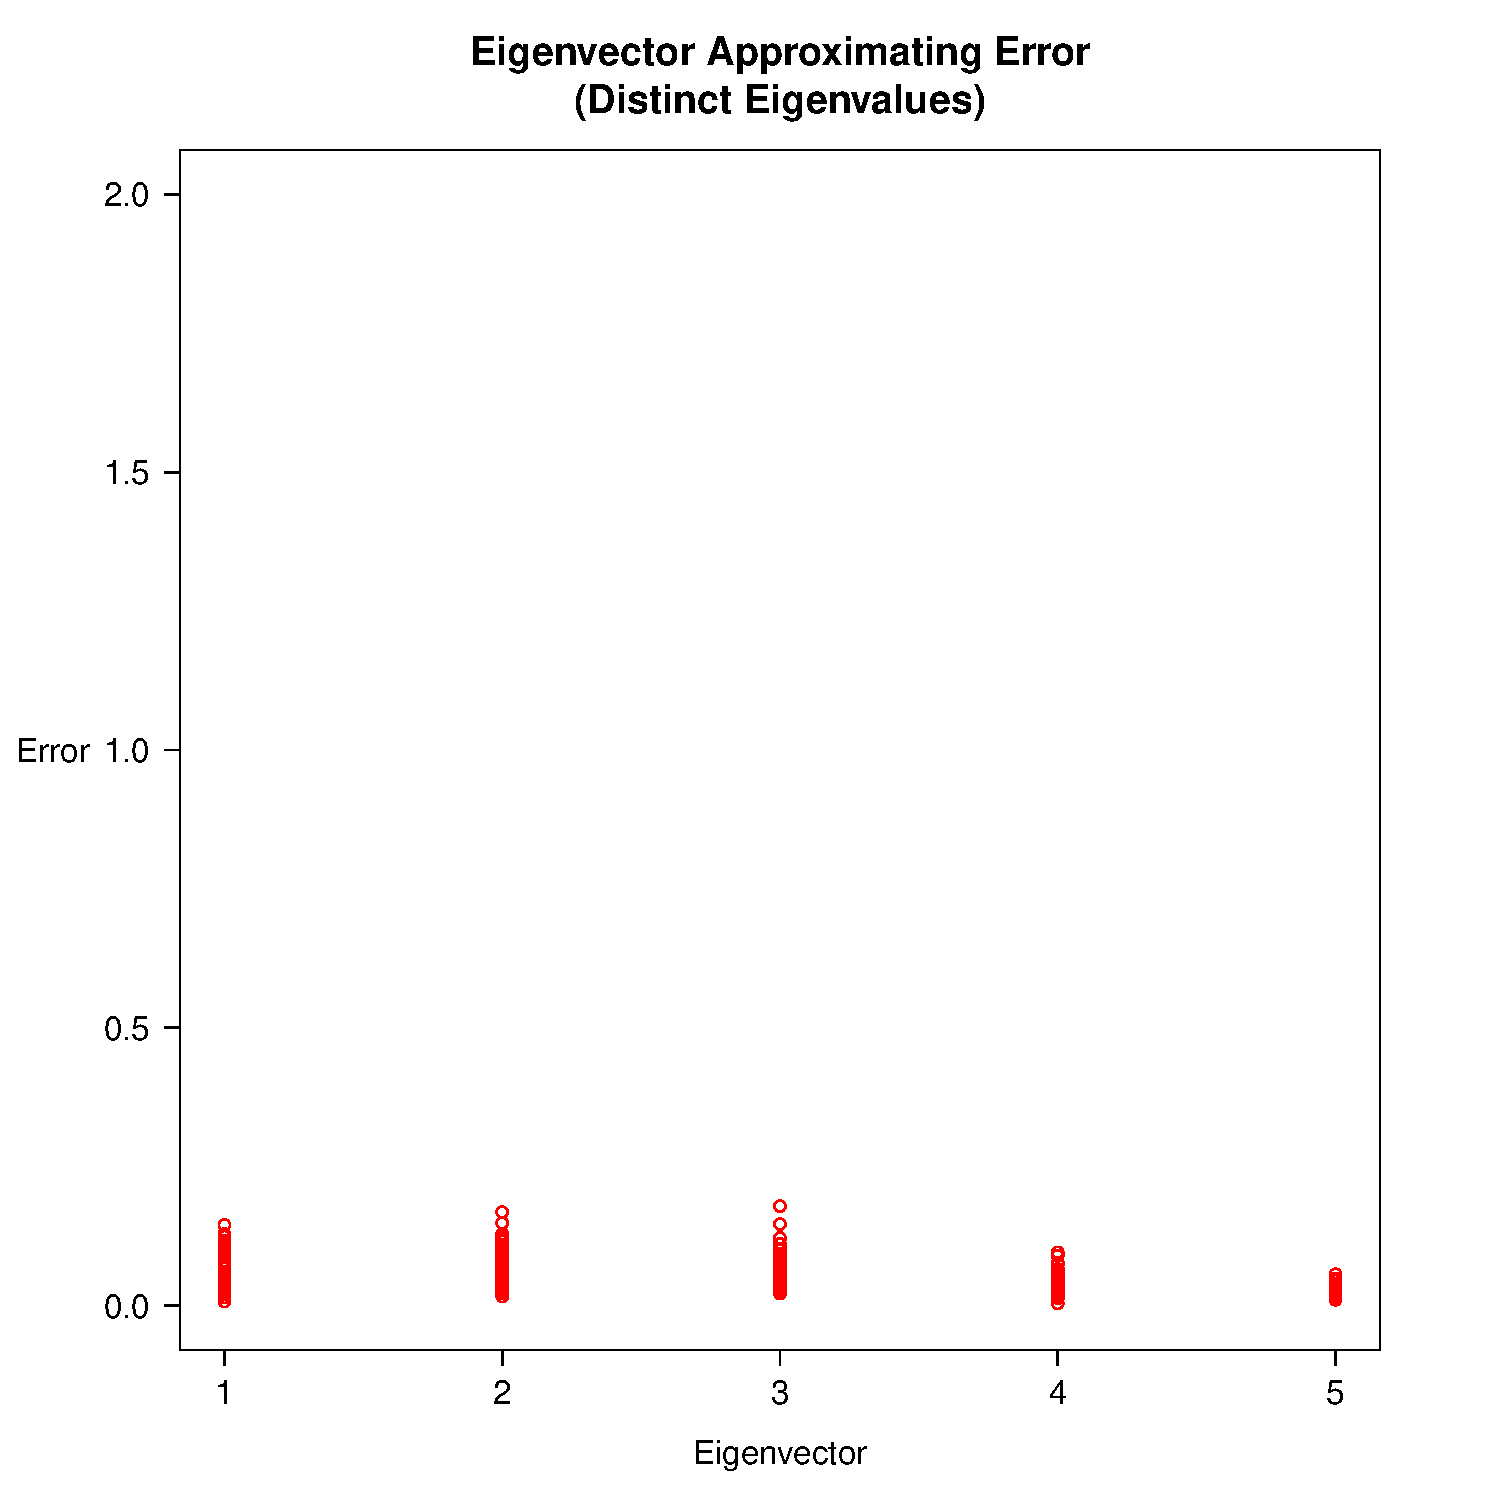
\includegraphics[scale=.43]{./Figures/diag_ex_2/e_vec_approx_diff.pdf}%
\figcaption{Deviations of the eigenvectors of $50$ sample covariance structures from the columns of the $5\times 5$ identity matrix. Each sample covariance matrix has an underlying structure of $diag(5,4,3,2,1)$ and a sample size of $n=5000$.}
\end{center}

\begin{center}
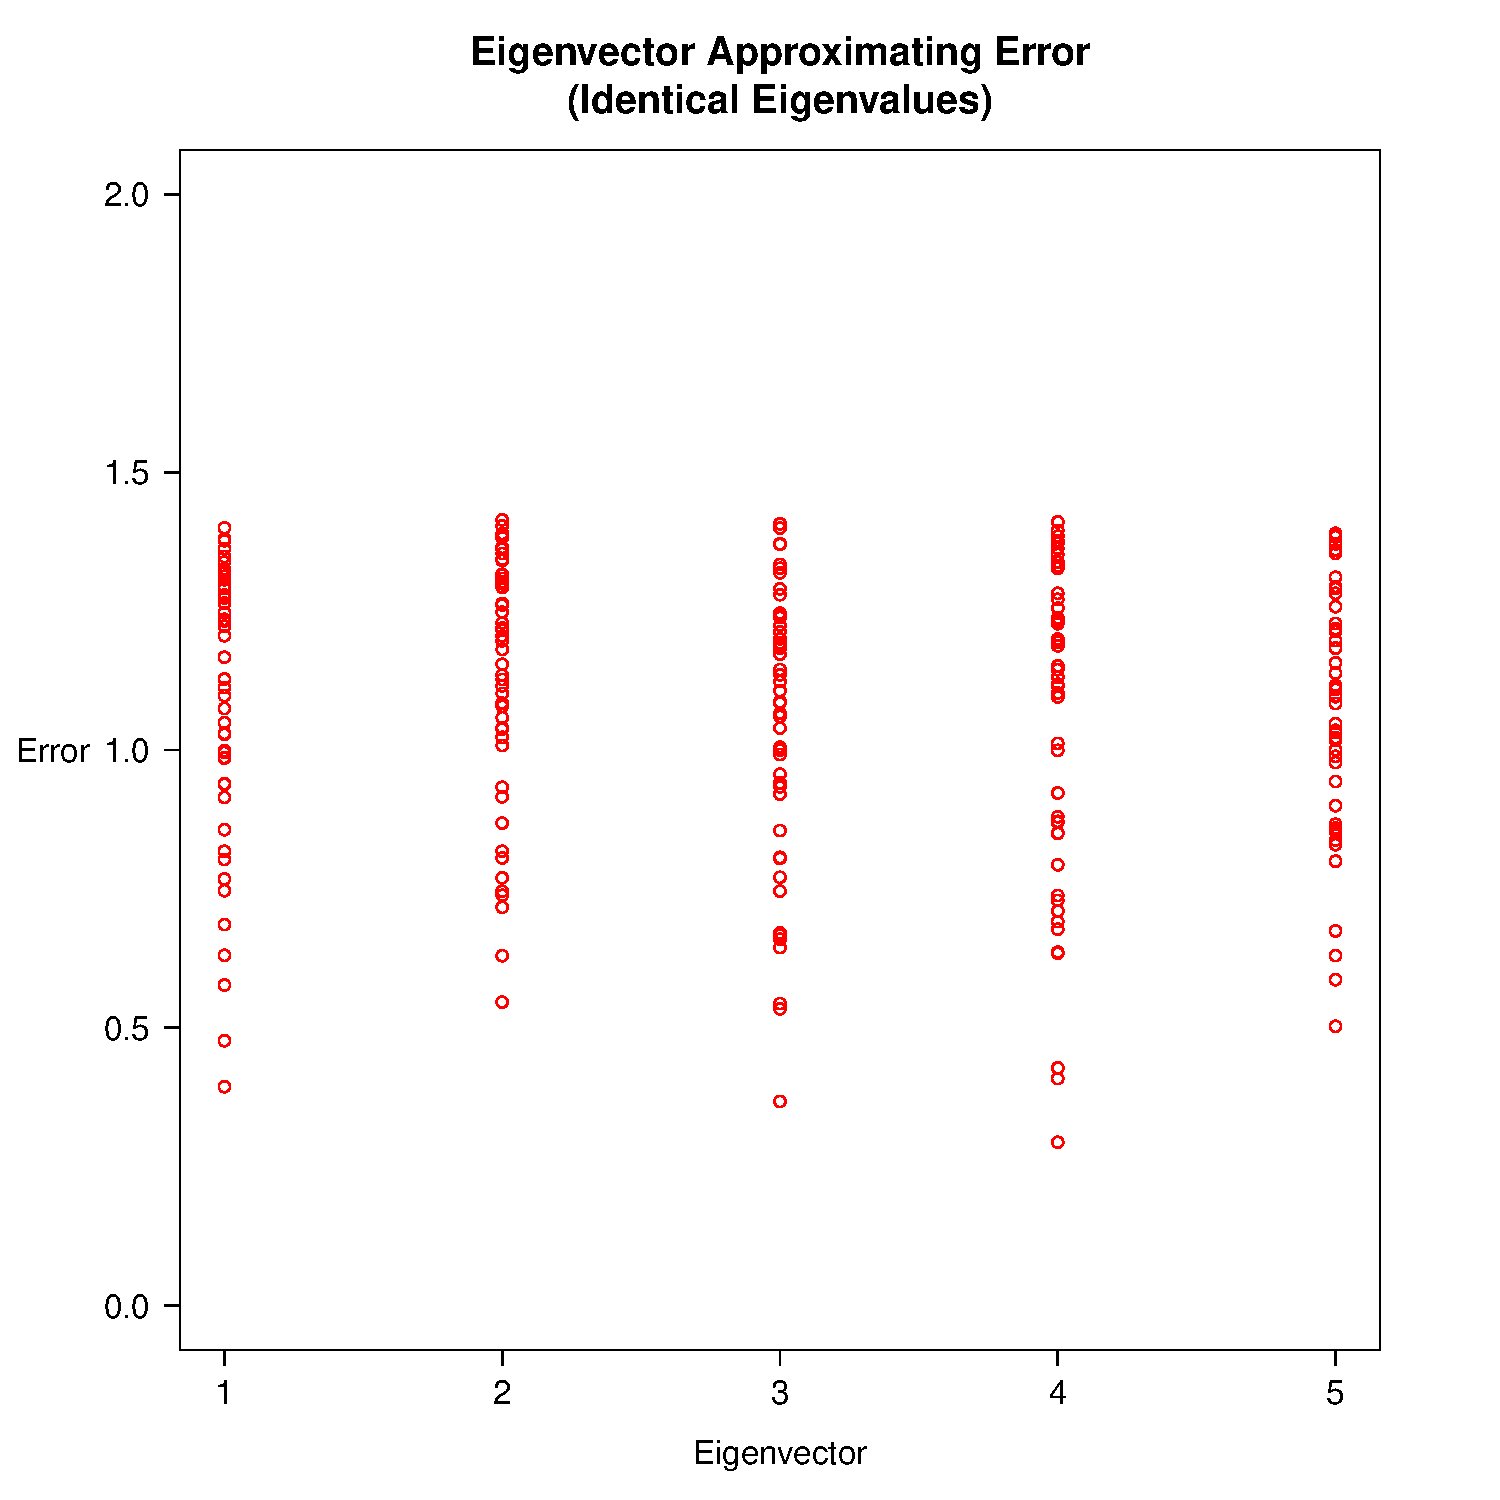
\includegraphics[scale=.43]{./Figures/diag_ex_2/e_vec_approx_same.pdf}%
\figcaption{Deviations of the eigenvectors of $50$ sample covariance structures from the columns of the $5\times 5$ identity matrix. Each sample covariance matrix has an underlying structure of $diag(1,1,1,1,1)$ and a sample size of $n=5000$.}
\end{center}
\newpage


\subsection{Leverage Scores}

Now we have good evidence that the eigenvectors of our sample covariance matrix $S$ are going to be close to the columns of the $5 \times 5$ identity matrix $I_5$. This means that 
$$
{\bf v_1}\approx\begin{bmatrix}1\\0\\0\\0\\0\end{bmatrix},{\bf v_2}\approx\begin{bmatrix}0\\1\\0\\0\\0\end{bmatrix},\ldots,{\bf v_5}\approx\begin{bmatrix}0\\0\\0\\0\\1\end{bmatrix}.
$$
Let's assume for the moment that these equalities are not approximate so that ${\bf v_i}={\bf e_i}$. If we run the CUR algorithm on such data with a rank parameter $k$ then the leverage score for the $i^{th}$ column is $1/k$ times the sum of the squares of the $i^{th}$ components of the first $k$ eigenvectors ${\bf v_1},\ldots,{\bf v_k}$. That is, running CUR with rank parameter $k$ we get
$$
\ell_i=\frac{1}{k}\left({\bf v_1}_i^2+\cdots+{\bf v_k}^2_i\right)
$$
where ${\bf v_j}_i$ is the $i^{th}$ component of the eigenvector ${\bf v_j}$. Now if ${\bf v_i}={\bf e_i}$ then 
$$
{\bf v_j}_i=
\begin{cases}
1& i={\bf j}\\
0& i \neq {\bf j}
\end{cases}
$$
and thus at most one of ${\bf v_1}_i,\ldots,{\bf v_k}_i$ is non-zero. Indeed if $i>k$ then all of the $\{{\bf v_j}_i\}$ zero and if $i<k$ then ${\bf v_i}_i=1$ and the rest of the $\{{\bf v_j}_i\}$ are zero. This means that if $i>k$ then $\ell_i=0$ and if $i\leq k$ then $\ell_i=1/k$.



To make this more clear we explicitly put the leverage scores in the following table.

\begin{center}
\begin{tabular}{|c||c|c|c|c|c|}
\hline&&&&&\\\text{}& Col. 1& Col. 2& Col. 3& Col. 4& Col. 5\\\hline\hline
$k=1$& 1& 0& 0& 0& 0\\\hline
$k=2$& 1/2& 1/2& 0& 0& 0\\\hline
$k=3$& 1/3& 1/3& 1/3& 0& 0\\\hline
$k=4$& 1/4& 1/4& 1/4& 1/4& 0\\\hline
$k=5$& 1/5& 1/5& 1/5& 1/5& 1/5\\\hline
\end{tabular}
\end{center}

While our eigenvectors aren't precisely the columns of $I_5$ they are close. Thus, as seen in Figure 4.12, the above calculations bare out in reality. Running CUR with a rank parameter of $k$ means that the leverage score of the first $k$ columns are about $1/k$ and the last $5-k$ columns are about zero. This plot was constructed in precisely the same manner as Figure 4.3. We have taken $N=10$ samples of multivariate normal data where each sample has $n=5000$ observations and an underlying covariance matrix $diag(5,4,3,2,1)$. We have then plotted the leverage scores for each sample for every value of $k$. The color correspondence of the figure is the same as that in Figure 4.3 and is given in the following table, 

\begin{center}
\begin{tabular}{|c|c|}
\hline&\\
column number& color\\\hline
1& red\\
2& blue\\
3& green\\
4& orange\\
5& black\\
\hline
\end{tabular} 
\end{center}




\newpage
\begin{center}
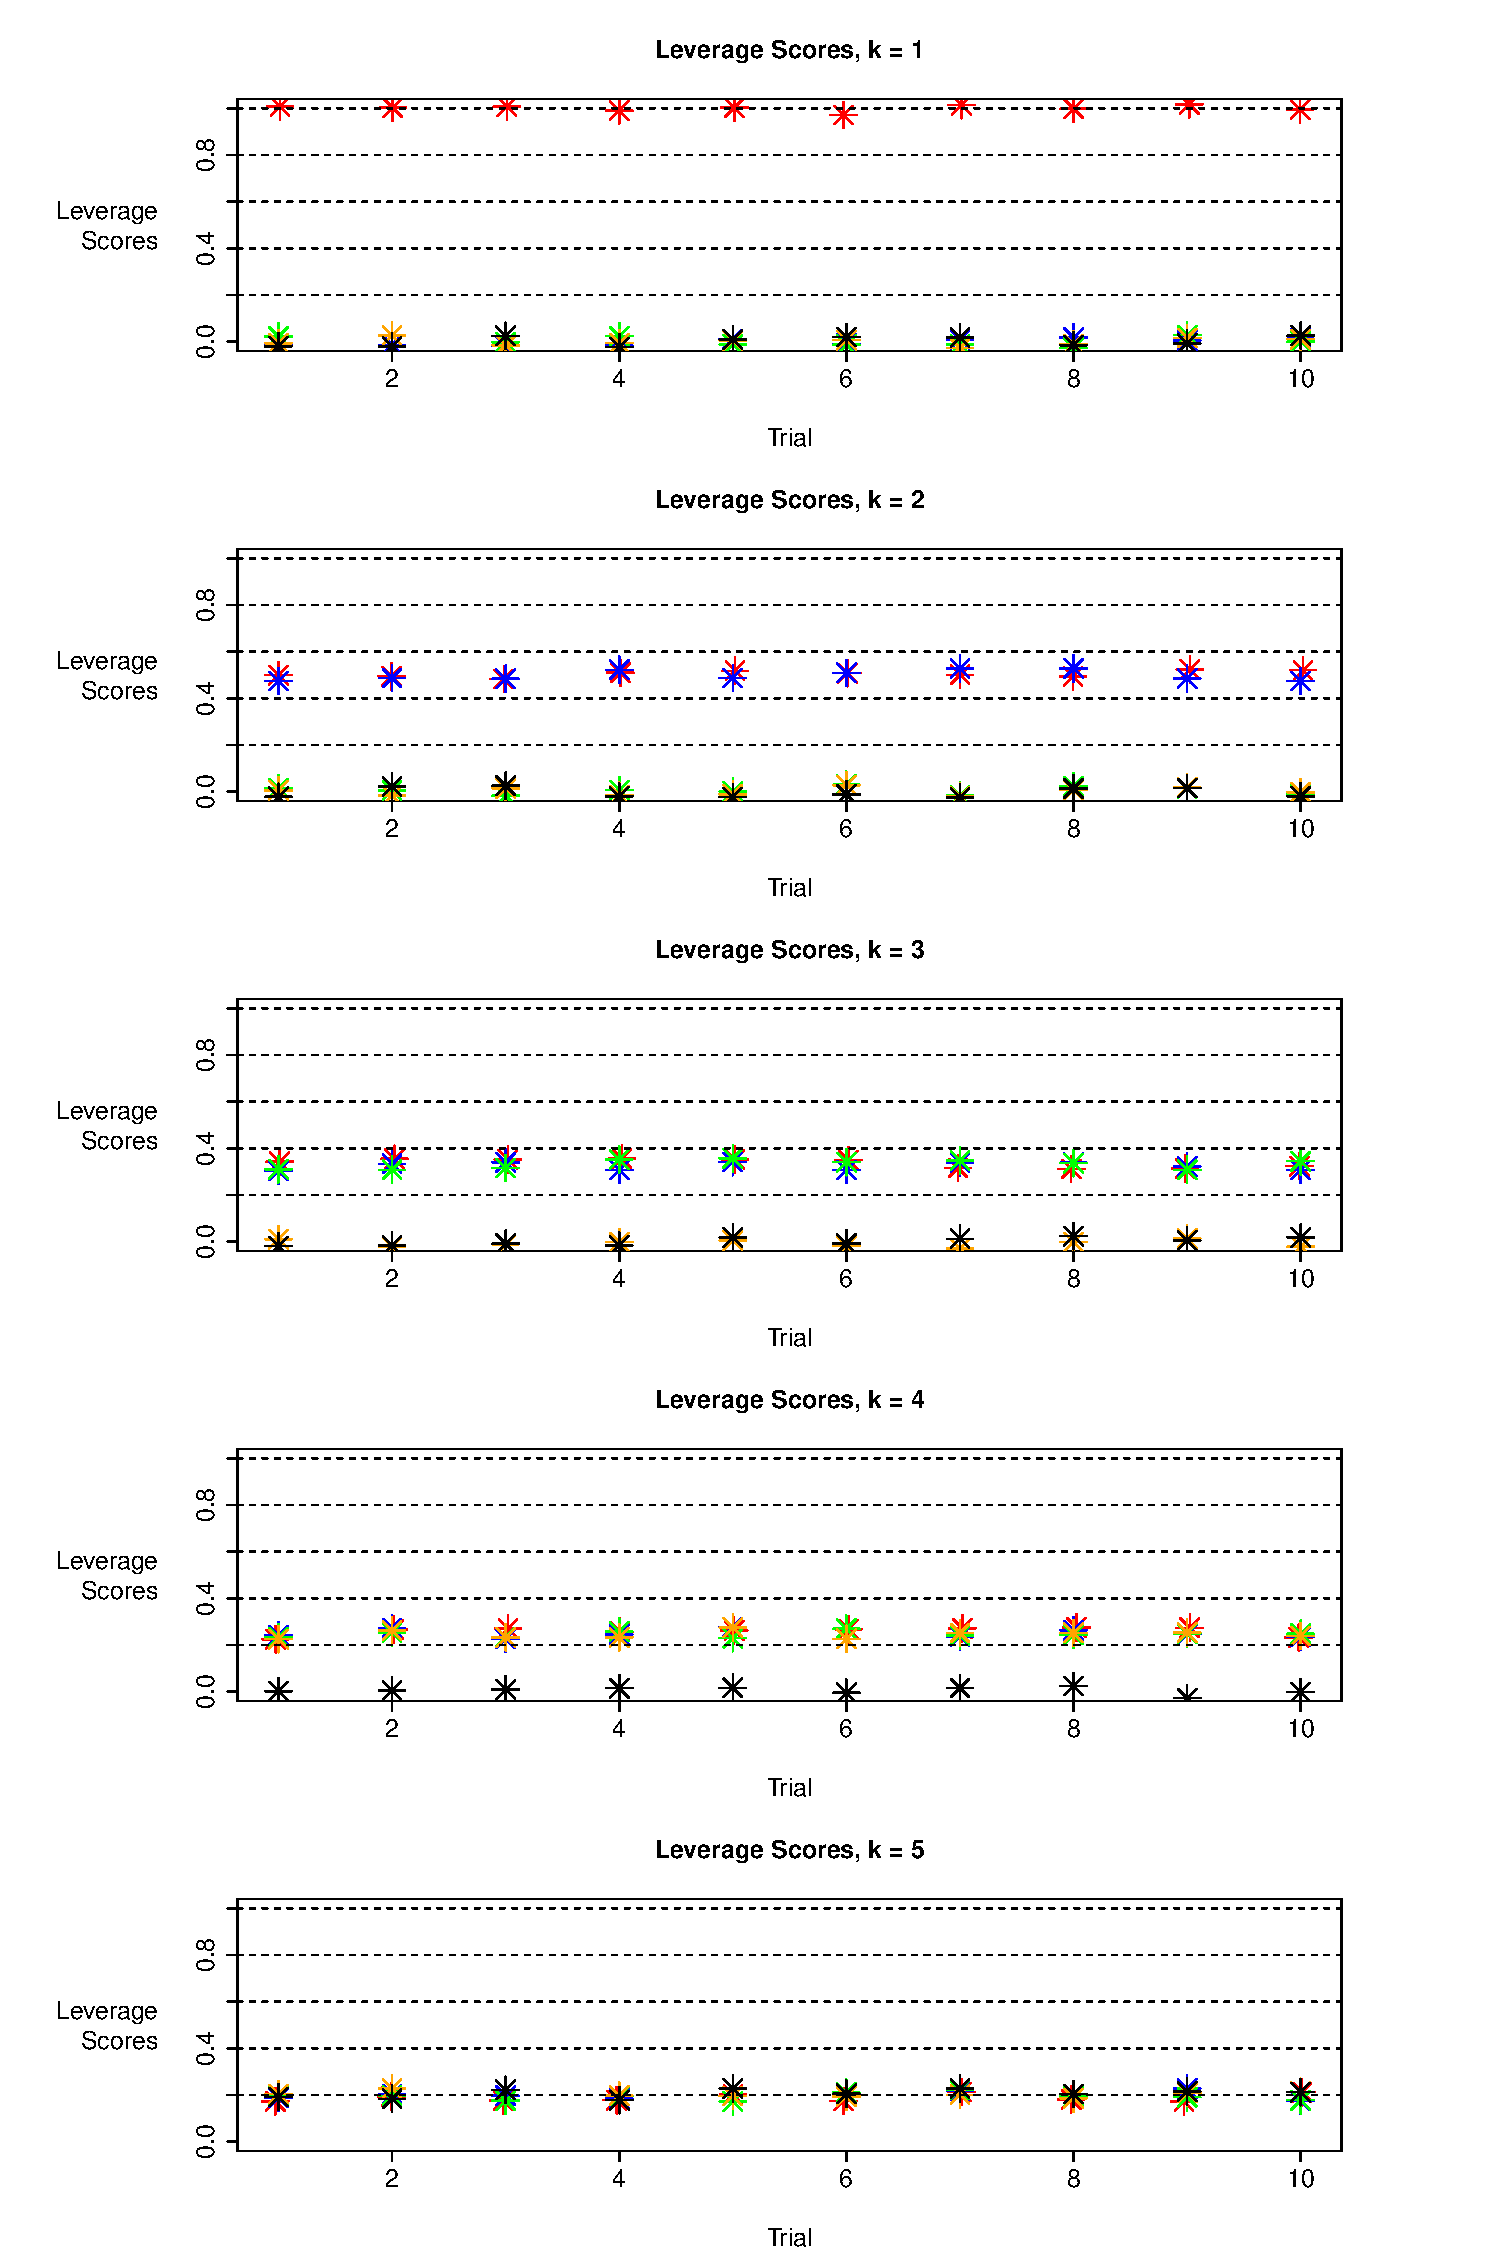
\includegraphics[scale=.6]{./Figures/diag_ex_2/levs.pdf}%
\figcaption{The leverage scores of data generated from a multivariate normal $N_5(0,diag(5,4,3,2,1))$ with sample sizes of N = 5000.}
\end{center}

\subsection{Columns Chosen}
The distribution of the leverage scores being what they are has an odd effect on the number of columns chosen by CUR. We want to say that for a column parameter $c$, 
$$
\text{E}\left[\mathscr{C}\right]\approx c.
$$
However from Figure 4.13 we can see that this is not true. Figure 4.13 is analogous to Figure $4.4$ in Example 1. In Figure 4.13 for each value of the rank parameter $k=1,\ldots,5$ we plot the average number of columns chosen by CUR (over $N=1000$ runs) for each value of the column parameter $c=0,\ldots,5$. That is, for each rank and column parameter pair $(c,k)$ we have run CUR on our data matrix 1000 times and recorded and plotted the average number of columns chosen.

Different from Example 1, the number of columns chosen by CUR from this data with underlying covariance matrix $diag(5,4,3,2,1)$ depends not only on $c$ but also on $k$. Temporarily let us ignore the case where $c=5$. When $c=5$ we will retain all of the columns of $X$ and thus $c=5$ implies $\mathscr{C}=5$ where $\mathscr{C}$ is the random variable representing the number of columns chosen by CUR. 

Let us look at the plots when $c \leq 4$. We then have two cases. When $c\leq 4$ and $c \leq k$ then we seem to choose $c$ columns. That is, our red dots seem to fall more or less on the blue line. However when $c\leq 4$ and $c > k$ then the graphs show us that we will choose precisely $k$ columns. Another way of saying this is that on average we choose about $min\{c,k\}$ columns. 

This behavior may be explained if we look back at our leverage scores. For a rank parameter of $k$ the leverage scores of the first $k$ columns are all about $1/k$ and the leverage scores of the remaining $5-k$ columns are $0$. Thus for $c<k$ if $i\leq k$ then
$$
c\ell_i\approx\frac{c}{k}<1.
$$
and if $i >k$ then $c\ell_i=0$. Thus generally all of the leverage scores will be less than $1$ and hence 
$$
\text{E}\left[\mathscr{C}\right]=\frac{c}{1-p_0}
$$
where $p_0$ is our failure probability as discussed in Chapter $3$. Thus the number of columns we will choose will be $c$ enhanced by the term $1/(1-p_0)$. We then will choose slightly more than $c$ columns. Note however that empirically we can see from the figure that when $c \leq k$ while the number of columns chosen is slightly above $c$ it isn't much above $c$. Indeed the average number of columns chosen still tracks closely with $c$. 

On the other hand if $c\geq k$ then for $i \leq k$
$$
c\ell_i\approx\frac{c}{k}\geq 1.
$$
and so we will generally keep the first $k$ columns with probability $1$. However when $c \geq k$ then $\ell_i=0$ for $i>k$ and so  we keep these last $5-k$ columns with probability $0$. Thus we will keep precisely $k$ columns. 


\newpage
\begin{center}
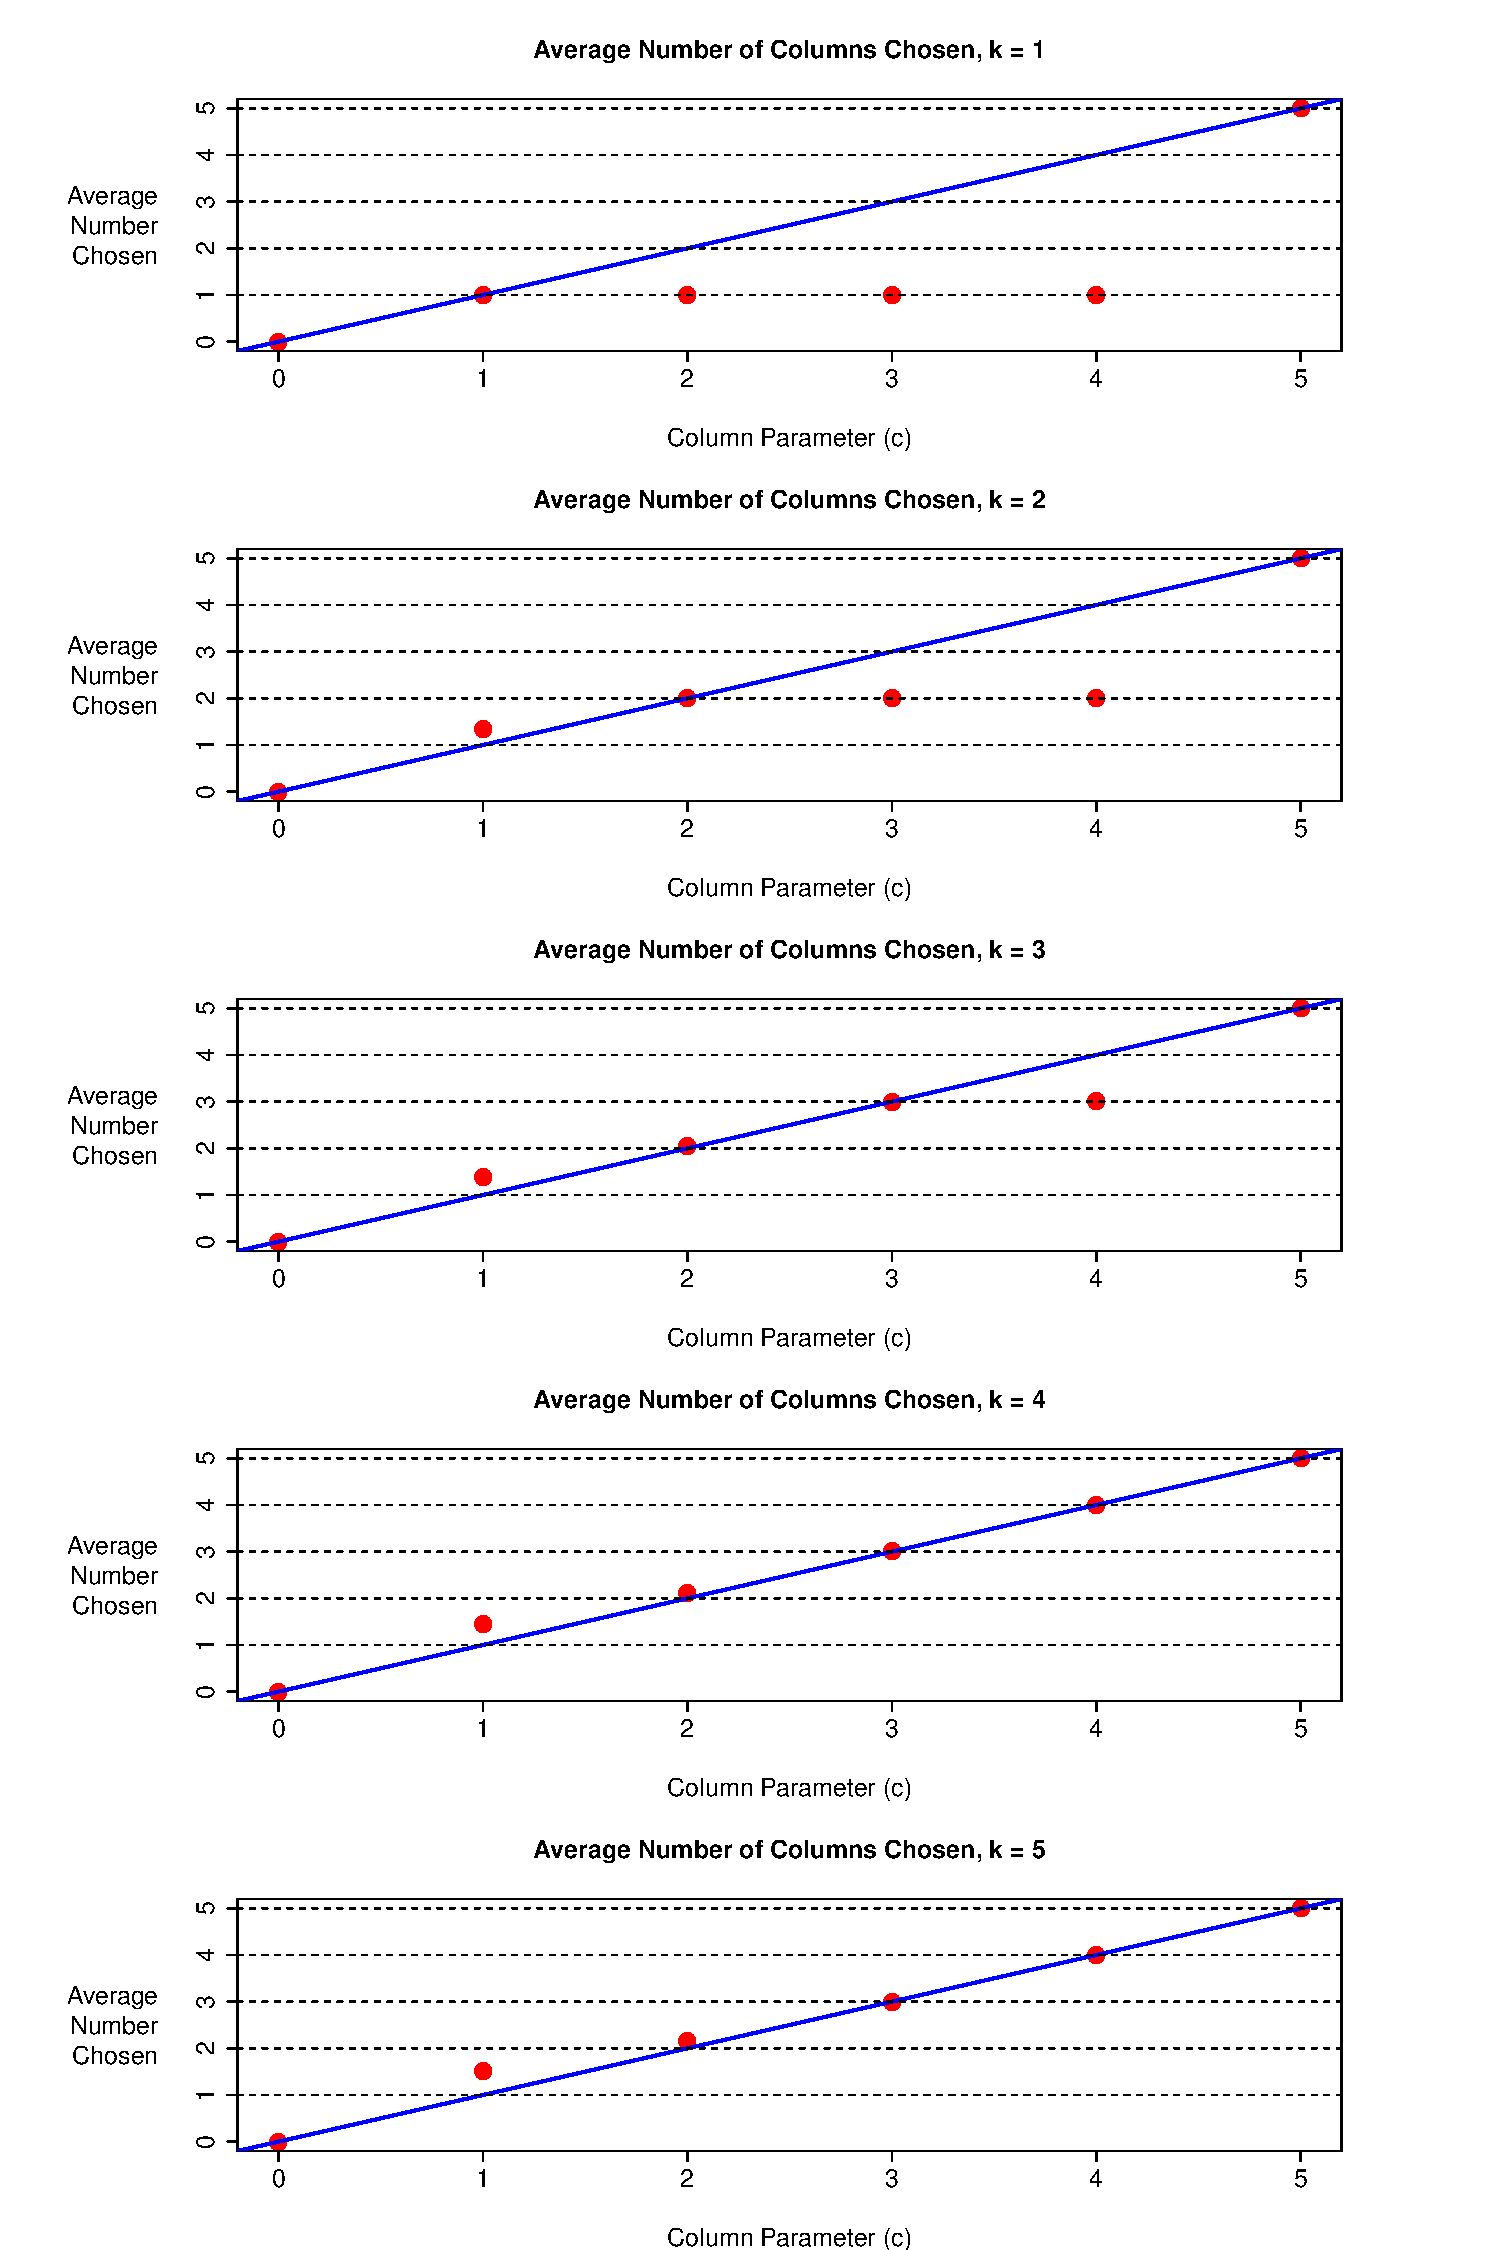
\includegraphics[scale=.60]{./Figures/diag_ex_2/chosen_v_c.pdf}%
\figcaption{The average ($N = 1000$) number of columns chosen for every permissible value of the rank and column parameters $c$ and $k$. The blue line has slope 1.}
\end{center}

\subsection{Effectiveness}

The last thing we would like to do in this example is evaluate the effectiveness of CUR relative to PCA. To this end in Figure 4.14 we plot the average effectiveness score (over $N=1000$ runs of CUR on our data) 
$$
e=\frac{||C||_F^2-||D||_F^2}{||X||_F^2}
$$
over every possible $(c,k)$ pair of rank and column parameters. 

\begin{center}
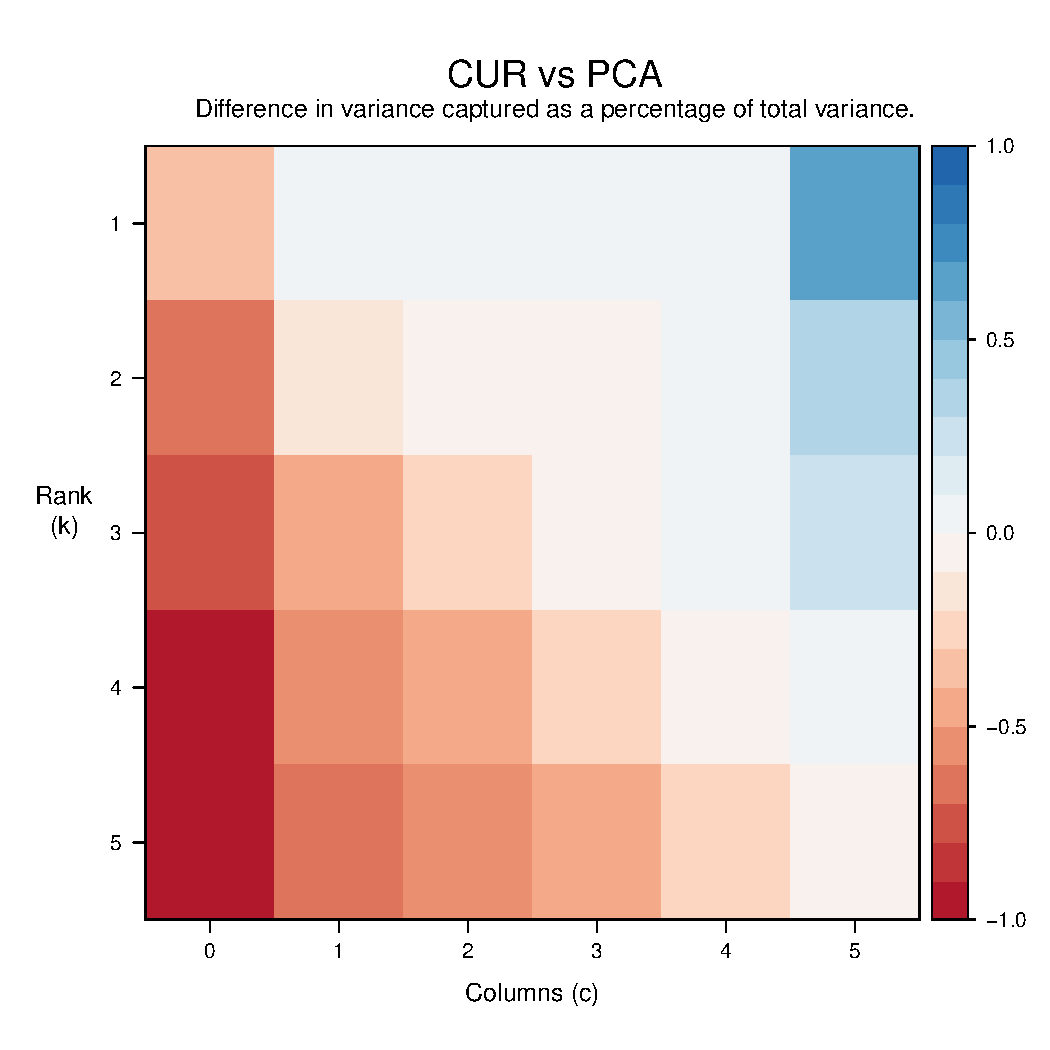
\includegraphics[scale=.63]{./Figures/diag_ex_2/raster.pdf}%
\figcaption{A plot of the average (N = 1000) effectiveness value e for each possible value of the rank and column parameters c and k.}
\end{center}

Compare this figure with the corresponding Figure 4.5 from Example 1. As in Figure 4.5 below the ``main diagonal'' of our graph (the line where $c=k$) principal components analysis does relatively better than CUR. Since below the main diagonal is when $c\leq k$ then CUR is choosing about $c$ columns here. As discussed at the end of Example 1 for theoretical reasons CUR will generally not be able to do better than PCA here. The general principle is that so long as we choose about $c$ columns when running CUR with column parameter $c$ then PCA will always do better than CUR when $c<k$. Note that when $c=k$ we have that CUR and PCA do about the same in terms of the effectiveness score. This is the same behavior observed in Figure 4.1 from Example 1.

However when $c>k$ we have behavior that deviates from that of our first example. Instead of CUR doing relatively better than PCA when $c>k$ we have that CUR does about as well as PCA in this region. To understand this behavior consider the plot in Figure 4.15. As in Figure 4.6 from Example 1 we plot we plot the first half of the effectiveness score
$$
\frac{||C||_F^2}{||X||_F^2}
$$
over all possible values of $c$ and $k$. This value is simply the percentage of total variance captured by CUR. 

There are two patterns we would like to explain in this figure. Let us ignore the last column of our plot because this corresponds to the case where $c=5$ and thus we choose all of the columns of the data matrix. If we do this then above the main diagonal of $c=k$ we have constant values across the rows of the figure. That is, for $k=1$ we have the same value for $1\leq c \leq 4$ and for $k=2$ we have the same value for $2 \leq c \leq 4$ and so forth. Furthermore as long as $c \geq k$ (i.e. we stay above the main diagonal) increasing $k$ increases the effectiveness of CUR. The plot becomes deeper blue and thus CUR captures more variance. Thus for the region of the graph where $c \geq k$ the variance captured by CUR increases as $k$ increases. However for the part of the graph where $c<k$ if we increase $k$ we, quite counter-intuitively, have the performance of CUR drop and, on average, CUR captures less variance. Thus below the main diagonal as $k$ increases the variance captured on average by CUR decreases. If we can understand these patterns in Figure 4.15 we will be well on our way to understanding CUR's performance on this data. 

\begin{center}
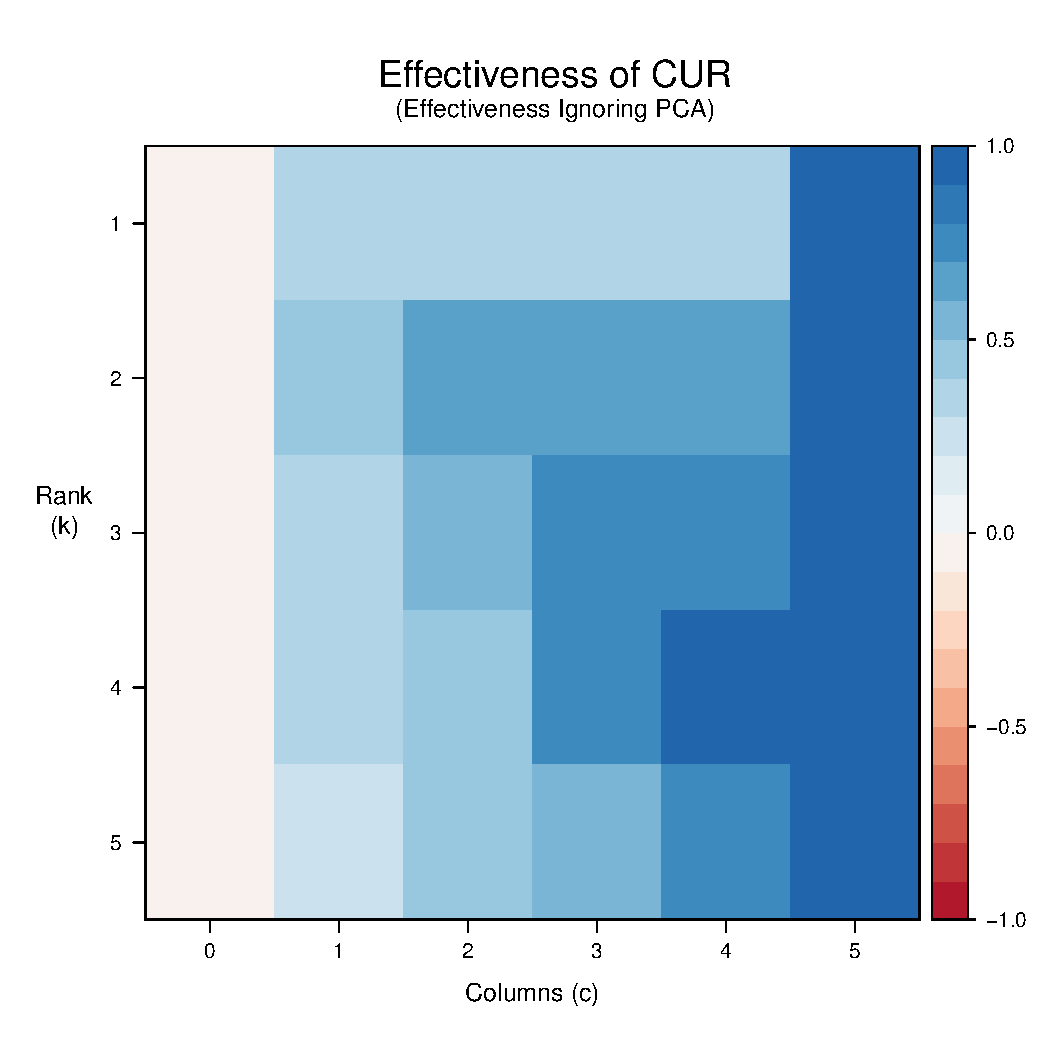
\includegraphics[scale=.63]{./Figures/diag_ex_2/raster_cur.pdf}%
\figcaption{A plot of the average percentage of variance captured by the CUR algorithm ($N=1000$) for each possible value of the rank and column parameters $c$ and $k$.}
\end{center}

To understand Figure 4.15 we need to revisit our plots of the leverage scores and the number of columns chosen in Figures 4.12 and 4.13 respectively. Note that in Figure 4.13 when $c<k$ we choose about $c$ columns and when $c \geq k$ we choose about $k$ columns. This follows because for a rank parameter $k$ there are $k$ non-zero leverage scores all approximately $1/k$ and thus if $c>k$ then
$$
c\ell_i\approx\frac{c}{k}>1
$$
and thus we choose each of the $k$ columns with non-zero leverage scores with probability $1$. The question now becomes which $k$ columns CUR will choose. As it turns out, CUR will simply choose the $k$ columns with the highest variances. Let's assume that the variances down the sample (and underlying population) covariance matrix are strictly decreasing along the main diagonal. If this is not true we can simply reorder the columns of our data matrix to make it so. Then, as noted earlier, we have that ${\bf v_i}\approx {\bf e_i}$. We then saw that for a rank parameter $k$ only the first $k$ leverage scores are non-zero (or not close to being zero). Since we have assumed that the columns are ordered in decreasing order according to variance then these first $k$ columns are precisely the $k$ columns with highest variance. 

Thus the reason that the rows of Figure 4.15 are constant so long as $c \geq k$ follows because, given a rank parameter $k$, CUR is choosing precisely the same subset of columns regardless of the value of $c$. Note however that if we increase $k$ yet still have that $c \geq k$ then we are increasing the number of columns CUR retains. Thus, as seen in Figure 4.15, the amount of variance captured by CUR increases as we increase $k$ so long as it remains that $c \geq k$. 

Now let us consider the region of Figure 4.15 where $c<k$. In this region we notice the odd pattern that increasing $k$ decreases, on average, the amount of variance captured by CUR. To understand this we to look closely at the relationship between the leverage scores of the columns and the amount of variance captured by the columns. Remember that the sample covariance matrix for our data is approximately the diagonal matrix $diag(5,4,3,2,1)$ and so the first column captures the most variance, the second captures the second most and so forth. Thus we would hope that the leverage scores of the columns reflect this relationship. 

To a degree the leverage scores of the columns do reflect their variance. For a rank parameter $k$ the only columns with non-zero leverage scores are the $k$ columns with the highest variances. In our example for $k=1$ we have that the first column (highest variance) is the only column with a non-zero leverage score. For $k=2$ we have that the first two columns are the only columns with non-zero leverage scores and so forth. Revisit Figure 4.12 to see this. 

Unfortunately the relationship between variance captured and the leverage scores could be better. Note that for any given rank parameter $k$ the non-zero leverage scores all have, approximately, the same value. It is true that given a rank parameter $k$ only the $k$ columns with the highest variances have positive leverage scores. However it is also true that all of the leverage scores are equal. Thus there is nothing in these importance scores to reflect the fact that one column has a higher variance than another. Given $k=2$ only $\ell_1$ and $\ell_2$ are positive, however $\ell_1=\ell_2=1/2$. %Thus given that $c<k$ then we retain about $c$ of the $k$ highest variance columns choosing each with the same probability.

This behavior of the leverage scores explains the pattern where increasing $k$ actually decreases the effectiveness of CUR. Consider keeping $c$ constant and increasing $k$ (so long as $c<k$). In this case we don't actually increase the number of columns we choose since still pick about $c$ columns. Remember in Figure 4.13 that we choose about $min\{c,k\}$ columns and thus if $c<k$ we will retain $c$ columns regardless of $k$. However as we increase $k$ we increase the number of columns with non-zero leverage scores and thus we increase the number of columns from which we choose. Thus by increasing $k$ we are allowing the algorithm to pick from columns with lower variances and, more importantly, we are choosing these lower variance columns with equal probability as our higher variance columns. So in a sense we are diluting the pool of columns from which we choose by adding in suboptimal columns and yet choosing these suboptimal columns with the same probability as more desirable columns. Thus, on average, the variance captured will decrease as $k$ increases because we will be increasing the probability of choosing columns with lower variances. 

For completeness we should now look at the corresponding effectiveness of PCA disregarding how CUR behaves. To see this we create Figure 4.16 plotting the value
$$
-\frac{||D||_F^2}{||X||_F^2}
$$
which is the other half of our effectiveness score $e$. The absolute value of the score plotted in Figure 4.16 is the percentage of variance captured by PCA. 

This figure is analogous to Figure 4.8 of Example 1. Remember that since $c$ is not a parameter of PCA then the performance of PCA is constant across the rows. Furthermore, as previously discussed,  PCA captures more variance as $k$ increases. Note however that unlike Example 1 here the relationship between $k$ and the amount of variance captured is not linear. In Figure 4.17 we plot this relationship. Notice that the increase in amount of variance captured by PCA decreases as $k$ increases. That is, the first principal components capture most of the variance. 

\newpage
\begin{center}
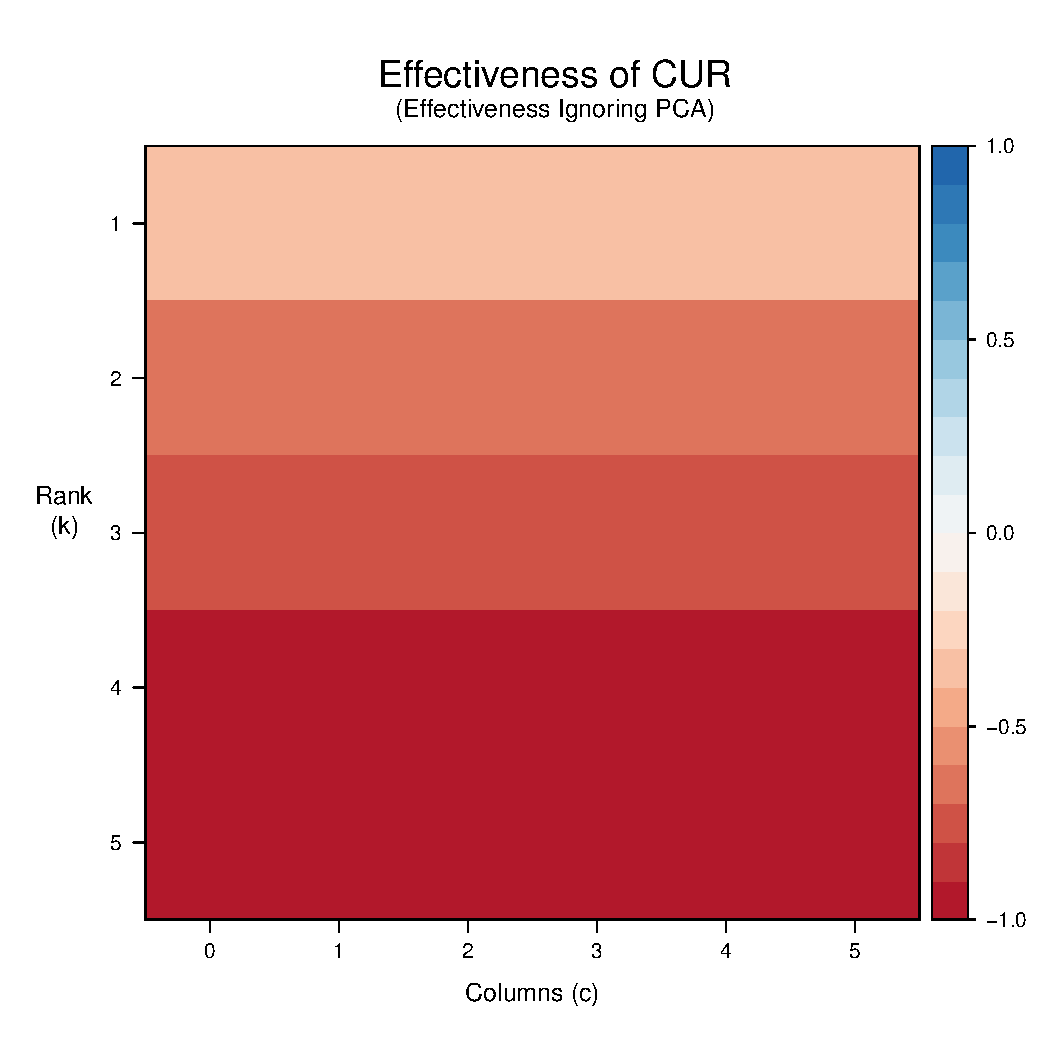
\includegraphics[scale=.57]{./Figures/diag_ex_2/raster_pca.pdf}%
\figcaption{A plot of the average percentage of variance captured by PCA ($N=1000$) for each possible value of the rank and column parameters $k$ and $c$.}
\end{center}

\begin{center}
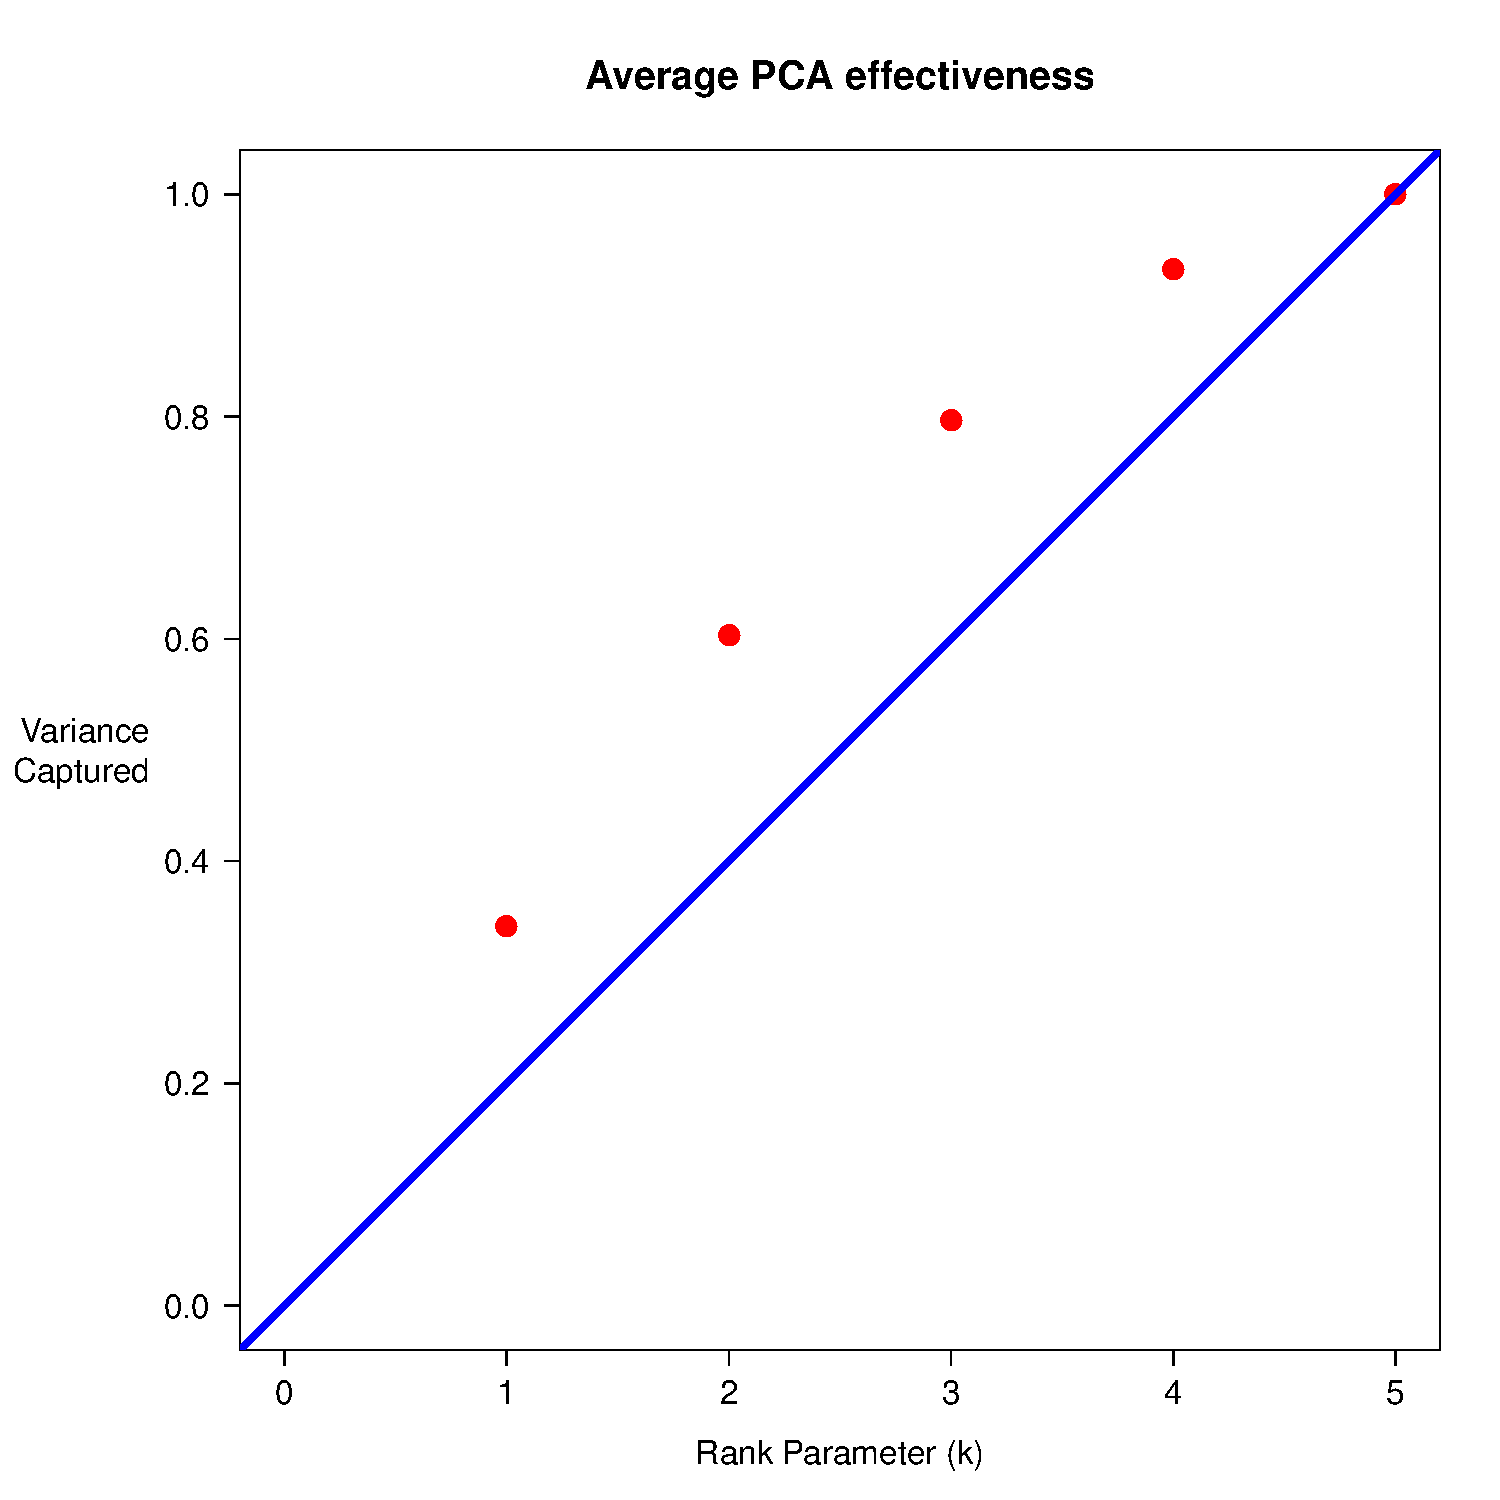
\includegraphics[scale=.4]{./Figures/diag_ex_2/avg_pca_effect.pdf}%
\figcaption{A plot of the average percentage of variance captured by PCA ($N=1000$) averaged across the different column parameter values. The blue line has a slope of $1$.}
\end{center}
\newpage

\subsection{Conclusion}
 
We see in this example again an emergent relationship between the rank and column parameters. The point of bifrucation seems, again, to be when $c=k$. When $c < k$ we have that CUR does relatively worse than PCA and when $c \geq k$ we have that CUR does about as well as PCA. Thus as we have previously concluded it seems that the best range of parameters in which to run CUR is when $c \approx k$. However this statement is even stronger than in Example 1. In this example when $c<k$ we have strange behavior where the larger the value of $k$ the worse CUR does and the better PCA does. Furthermore PCA will generally capture more variance than CUR in this region. Thus we really don't want $c<k$. However taking $c>k$ does not gain us anything over taking $c=k$. Indeed CUR does not capture more variance for these values of $c$. Thus there is no reason to choose $c>k$. The conclusion, based on Example 2, is then that for data with diagonal covariance structure having distinct eigenvalues if we are going to run CUR on the data to select columns we should have $c=k$. In this case CUR will do about as well as PCA in capturing the variance present in the data.  




\newpage
%%%%%%%%%%%%%%%%%%%%%%%%%%%

\section{Example 3: Compound Symmetric}

Now we have looked at how CUR performs in comparison to PCA on a data with covariance matrix having one repeated eigenvalue. Similarly we have looked at CUR in comparison to PCA on data with a covariance matrix having no repeated eigenvalues. It would seem to make most sense to look at data where the covariance matrix has some repeated eigenvalues as well as some distinct. Instead of using, say, $diag(5,4,3,3,3)$, as an example of such a covariance matrix we are going to consider a class of covariance matrices called compound symmetric. Our example will then allow us to see what happens when some, but not all, of our eigenvalues are repeated as well as highlight some features of CUR we would not see using a diagonal covariance structure. 

The term compound symmetry comes from the ANOVA literature and means that the covariances among pairs of variables are equal. That is, if $\Sigma$ is the covariance matrix of our $p$--dimensional random vector $\rv{X}=(\mathscr{X}_1,\ldots,\mathscr{X}_p)^T$ then 
$$
\Sigma=
\begin{bmatrix}
\sigma_{\mathscr{X}_1}^2& \sigma& \sigma& \cdots& \sigma\\
\sigma& \sigma_{\mathscr{X}_2}^2& \sigma& \cdots& \sigma\\
\sigma& \sigma& \ddots& & \vdots\\
\vdots& \vdots& &\ddots& \sigma\\
\sigma& \sigma& \cdots& \sigma &\sigma_{\mathscr{X}_p}^2
\end{bmatrix}
$$
where $\sigma_{\mathscr{X}_1}^2,\sigma_{\mathscr{X}_2}^2,\ldots,\sigma_{\mathscr{X}_p}^2$ are the variances of $\mathscr{X}_1,\ldots,\mathscr{X}_p$ and $\sigma$ is the common covariance among them. 

It turns out that the compound symmetric covariance structure has simple closed forms for its eigenvalue and eigenvectors if we have that all that variances are equal to one such that $\sigma_{\mathscr{X}_1}^2=\sigma_{\mathscr{X}_2}^2=\cdots=\sigma_{\mathscr{X}_p}^2=1$. We can think of this as working with the correlation matrix. For a common correlation $\rho$ such a matrix is in the following form,
$$
\Sigma=
\begin{bmatrix}
1& \rho& \rho& \cdots& \rho\\
\rho& 1& \rho& \cdots& \rho\\
\rho& \rho& \ddots& & \vdots\\
\vdots& \vdots& &\ddots& \rho\\
\rho& \rho& \cdots& \rho &1
\end{bmatrix}.
$$
This correlation structure is quite simple. Every variable has precisely the same correlation with every other variable. They all have the same correlations and variances.

Note that this is similar to our first example of $\Sigma=I_5$. There was no way to pick a ``good'' subset of variables. However there is also no way to pick a ``bad'' set of variables. In terms of capturing variance of the data the performance of the CUR algorithm will directly be a product of \emph{how many} variables are chosen. After all, for a fixed size there is no reason to prefer one subset over another. If CUR chooses $m$ of the variables then it will capture $\frac{m}{p}$ percentage of the variance. This follows because each of the $p$ variables has a variance of $1$ and thus the total variance of the data is $p$. 

A very attractive feature of such covariance matrices is that it is possible to predict precisely what PCA will do with data having this covariance structure because the eigen-structure of compound symmetric correlation matrices is known. Let us review some known facts about compound-symmetric matrices. We take these facts from \cite{johnson}. For $\rho>0$ the first eigenvalue will be 
$$
\lambda_1=1+(p-1)\rho
$$ 
and its associated eigenvector will be 
$$
{\bf v_1}=\frac{1}{\sqrt{p}}(1,\ldots,1)^T
$$
meaning the first principal component will account for 
$$
\rho+\frac{1-\rho}{p}
$$ 
percentage of the total variance. The remaining $p-1$ eigenvalues will be $\lambda_{i}=1-\rho$ for $i=2,\ldots,p$ and one choice of associated eigenvectors is to have
$$
{\bf v_i}=\frac{1}{\sqrt{i(i-1)}}
\begin{bmatrix}
1\\
\vdots\\
1\\
-(i-1)\\
0\\
\vdots\\
0
\end{bmatrix}
$$
for $i>2$ such that the first $i-1$ components of ${\bf v_i}$ are $\frac{1}{\sqrt{i(i-1)}}$, the $i^{th}$ components is $\frac{-(i-1)}{\sqrt{i(i-1)}}$ and the remaining components are zero. We say this is one choice because all of these eigenvalues are repeated and thus we will have an infinite number of choices for the eigenvectors ${\bf v_i}$ for $i\geq2$. This means that the $i^{th}$ principal component for $i>2$ will account for 
$$
\frac{1-\rho}{p}
$$ 
fraction of the total variance. Let us look at some data to see if our hunches about the performance of CUR and PCA are correct. 

\subsection{The Data}

Consider $\rv{X}$ to be a multivariate normally distributed random vector containing $p=5$ components. Let the underlying covariance structure of $\rv{X}$ be a compound symmetric covariance matrix with unit variances (i.e. a correlation matrix) and common correlations among the variables of $\rho=.7$. That is, if $\Sigma$ is our underlying covariance structure then
$$
\Sigma=
(.7){\bf 1}{\bf 1}^T+(.3)I=\begin{bmatrix}
1& .7& .7& .7& .7\\
.7& 1& .7& .7& .7\\
.7& .7& 1& .7& .7\\
.7& .7& .7& 1& .7\\
.7& .7& .7& .7& 1
\end{bmatrix}.
$$
As previously we create a variable-mean centered $n \times p$ data matrix $X$ consisting of $n=5000$ observations of $\rv{X}$. 

The sample covariance matrix $S$ is
$$
S=
\begin{bmatrix}
0.97& 0.68& 0.69& 0.69& 0.68\\
0.68& 0.98& 0.7& 0.69& 0.68\\
0.69& 0.7& 1.02& 0.71& 0.7\\
0.69& 0.69& 0.71& 1.01& 0.7\\
0.68& 0.68& 0.7& 0.7& 1
\end{bmatrix}
$$
which deviates from $\Sigma$ by only $.5\%$ as a percentage of $||\Sigma||_F$ since
$$
\frac{||\Sigma-S||_F}{||\Sigma||_F}=.005.
$$
Thus our sample data $X$ should be a good representation of $\rv{X}$. 

\newpage
\subsection{Eigenvectors}

Now by our previous discussion since $\Sigma$ is compound symmetric with $\rho=.7$ then the first eigenvalue will be
$$
\lambda_1=1+(p-1)\rho=1+(5-1)(.7)=3.8
$$
and the remaining $4$ eigenvalues will be 
$$
\lambda_{2}=\lambda_3=\lambda_4=\lambda_5=1-\rho=.3.
$$
Since $S$ is a good approximation of $\Sigma$ then we expect the eigenvalues of $S$ to be similar to those of $\Sigma$. Indeed the eigenvalues of $S$ are
$$
\begin{aligned}
\lambda_1&=3.764\\ \lambda_2&=0.314\\ \lambda_3&=0.305\\ \lambda_4&=0.303\\ \lambda_5&=0.292
\end{aligned}
$$
and thus the same pattern of eigenvalues is borne out in the sample matrix. 

The first eigenvalue is distinct and the remaining $4$ eigenvalues are nearly equal. As we have discovered the eigenvector associated with $\lambda_1$ will be well determined and the eigenvectors associated with $\lambda_2$ through $\lambda_5$ will not. Now by our introductory discussion we know that the first eigenvector ${\bf v_1}$ of $\Sigma$ is
$$
{\bf v_1}=\frac{1}{\sqrt{p}}
\begin{bmatrix}
1\\
1\\
1\\
1\\
1
\end{bmatrix}
$$
and for $i=2,\ldots,5$ the remaining eigenvectors can be arranged such that 
$$
{\bf v_i}=\frac{1}{\sqrt{i(i-1)}}
\begin{bmatrix}
1\\
\vdots\\
1\\
-(i-1)\\
0\\
\vdots\\
0
\end{bmatrix}.
$$


Then in Figure 4.18 we make a plot similar to those in Figures 4.10 and 4.11. We generated $50$ sample data matrices similar to $X$ and for each computed the eigenvectors of the associated sample covariance matrix. Then for any such sample matrix if ${\bf u_1},\ldots,{\bf u_5}$ are the sample eigenvectors we compute for $i=1,\ldots, 5$ the distance or error of ${\bf u_i}$ approximating ${\bf v_i}$ as
$$
error=||{\bf u_i}-{\bf v_i}||
$$
and plot it as the point $(i,error)$ in Figure 4.18. 

Looking at Figure 4.18 our intuition is justified. We have that the first eigenvector of the samples is always very close to ${\bf v_1}=\frac{1}{\sqrt{5}}(1,\ldots,1)^T$ while the remaining eigenvectors vary greatly. As we have done previously let us look at what this means for the leverage scores of such data matrices. 

\newpage
\begin{center}
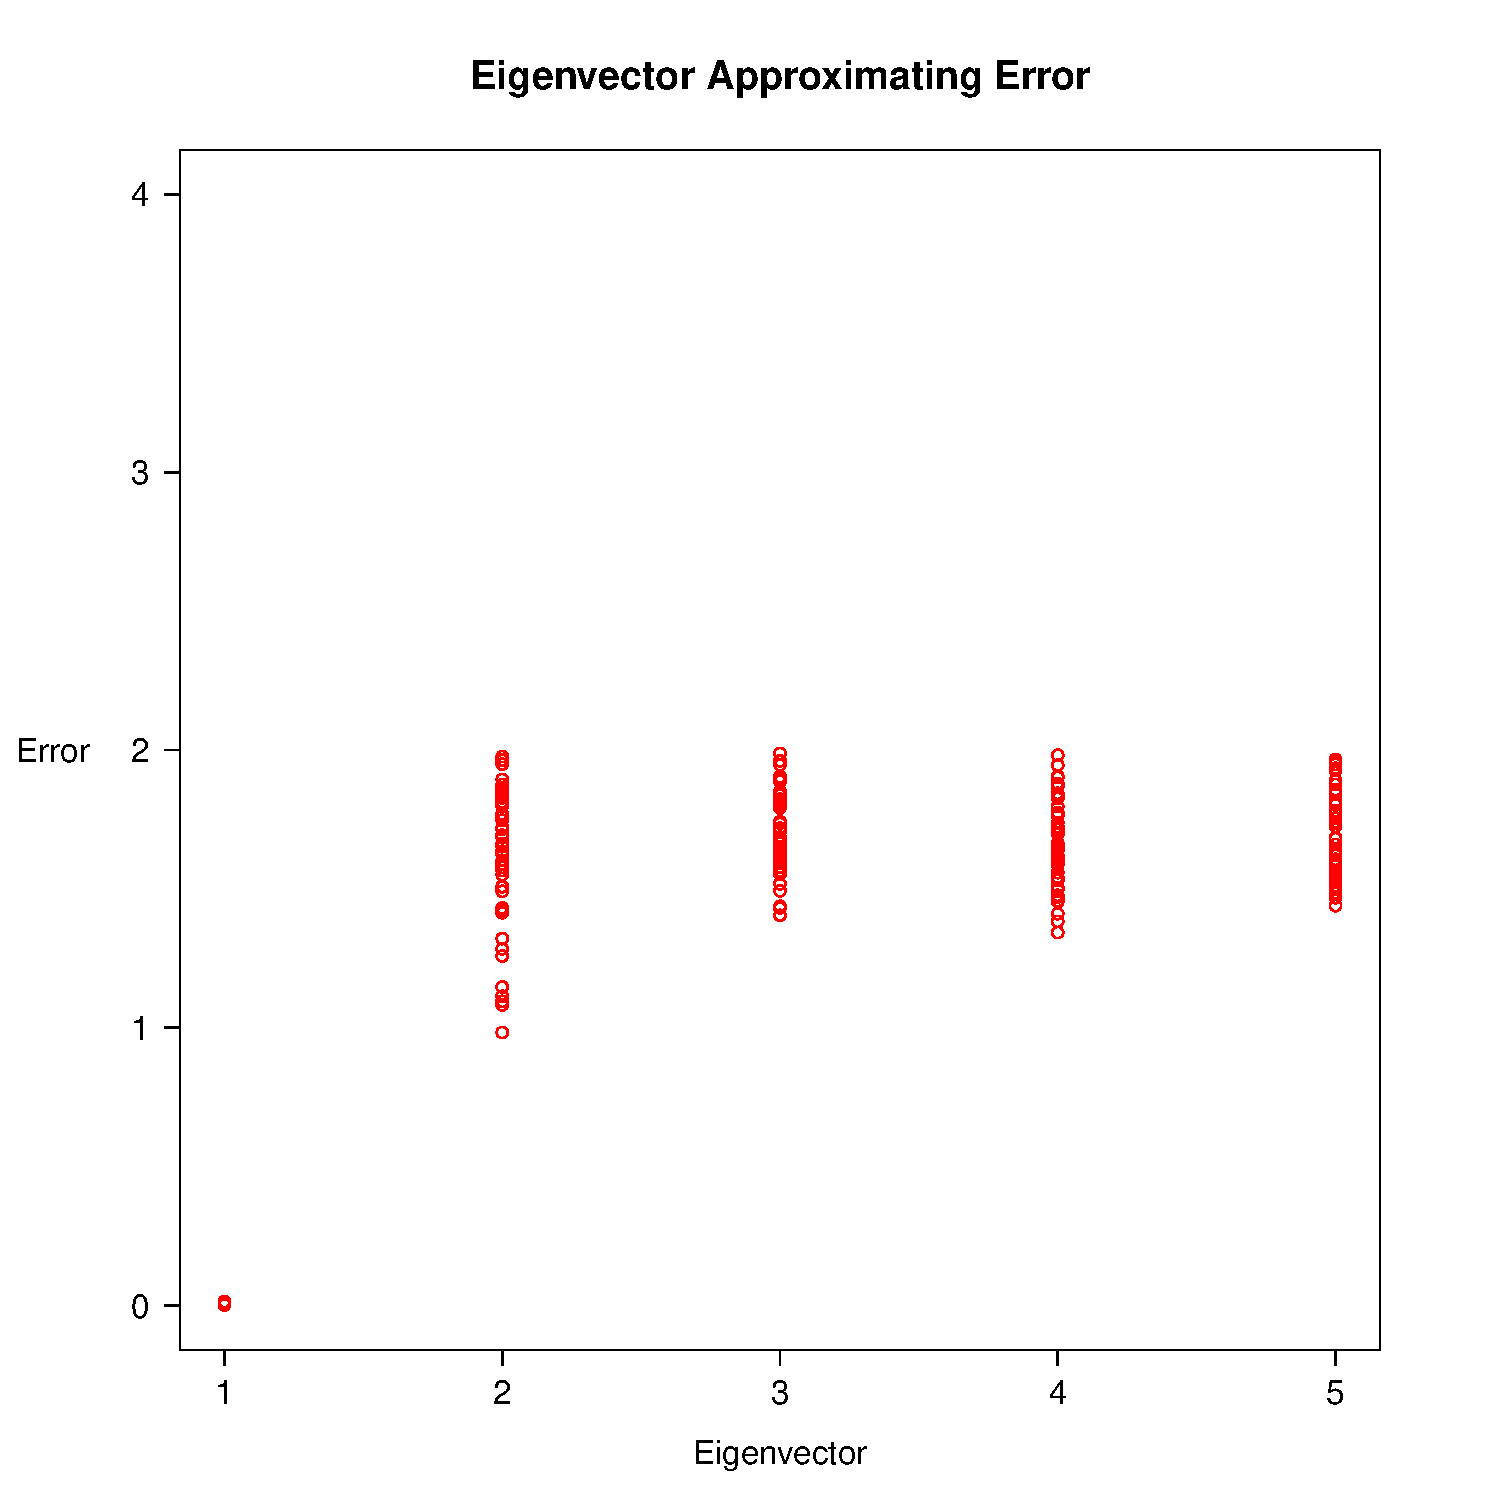
\includegraphics[scale=.53]{./Figures/cs_ex_1/eigen.pdf}
\figcaption{Deviations of the eigenvectors of $50$ sample covariance structures from their theoretical values. Each sample covariance matrix is from an $5000 \times 5$ data matrix with underlying covariance structure that is a compound symmetric correlation matrix with common correlation of $.7$.}
\end{center}



\newpage
\subsection{Leverage Scores}

In Figure 4.19 we generated 10 sample $5000 \times 5$ data matrices of $\rv{X}$ and for each value of $k$ we have plotted the leverage score of the columns of each sample. This should be a familiar plot by now. Once again the correspondence of the colors is 

\begin{center}
\begin{tabular}{|c|c|}
\hline&\\
column number& color\\\hline
1& red\\
2& blue\\
3& green\\
4& orange\\
5& black\\\hline
\end{tabular} 
\end{center}

For the first plot in Figure 1.19 we can see that for all $10$ data matrices the leverage scores of all of the columns are equal to $.2=1/5$. We can understand this because the leverage scores of the columns for a rank parameter of $k=1$ are simply the squares of the components of the first eigenvector ${\bf v_1}$. However since ${\bf v_1}\approx\frac{1}{\sqrt{5}}(1,\ldots,1)^T$ then 
$$
\ell_i\approx{\bf v_1}_i^2=\left(\frac{1}{\sqrt{5}}\right)^2=\frac{1}{5}.
$$
Since the eigenvalue for this first eigenvector is distinct from the other eigenvalues of $S$ and consequently ${\bf v_1}$ is well determined then it should generally be true that for $K=1$ and for any $i=1,\ldots,5$ we will have that $\ell_i\approx 1/5$.

However for $k>1$ we compute the leverage scores for the columns using not only ${\bf v_1}$ but also the eigenvectors ${\bf v_2},\ldots,{\bf v_k}$. However as we saw in our first example since the eigenvalues associated with these latter $k-1$ eigenvectors are all nearly equal then the components of these eigenvectors are quite arbitrary. Thus we expect including the components of the eigenvectors ${\bf v_2},\ldots,{\bf v_k}$ will introduce quite a bit of arbitrary variability into the leverage scores. This should be reminiscent as we discussed it at length in Example 1.

We can see this phenomena in Figure 4.19. Looking at the plots corresponding to $k>1$ we can not distinguish a pattern to the leverage scores. The plots look similar to those of Example 1 in Figure 4.3. The seemingly random behavior of the leverage scores is due to the arbitrary components introduced into the leverage scores from the eigenvectors associated with the common eigenvalue $1-\rho=.3$.

\subsection{Columns Chosen}

Next we want to look at how many columns the CUR algorithm chooses for different combinations of our rank and column parameters $k$ and $c$. Thus in Figure 4.20 for each rank parameter $k=1,\ldots,5$ we plot the average number of columns chosen by CUR for each value of the column parameter $c=0,\ldots,5$. 

Note that in Figure 4.20 we see that the average number of columns chosen by CUR tracks very closely with the column parameter $c$. This is very nice because if $\mathscr{C}$ is the random variable representing the number of columns chosen by CUR then 
$$
\text{E}\left[\mathscr{C}\right]\approx c.
$$
Once again we can then think of $c$ as controlling for, on average, how many columns CUR will retain. 

%We can explain this behavior by looking back at the leverage scores in Figure 4.19. Note that the leverage scores tend to cluster around $1/5$ and are thus quite small. Note that for any value of $k$ the leverage scores tend to be less than or equal to $1/k$.  

\newpage
\begin{center}
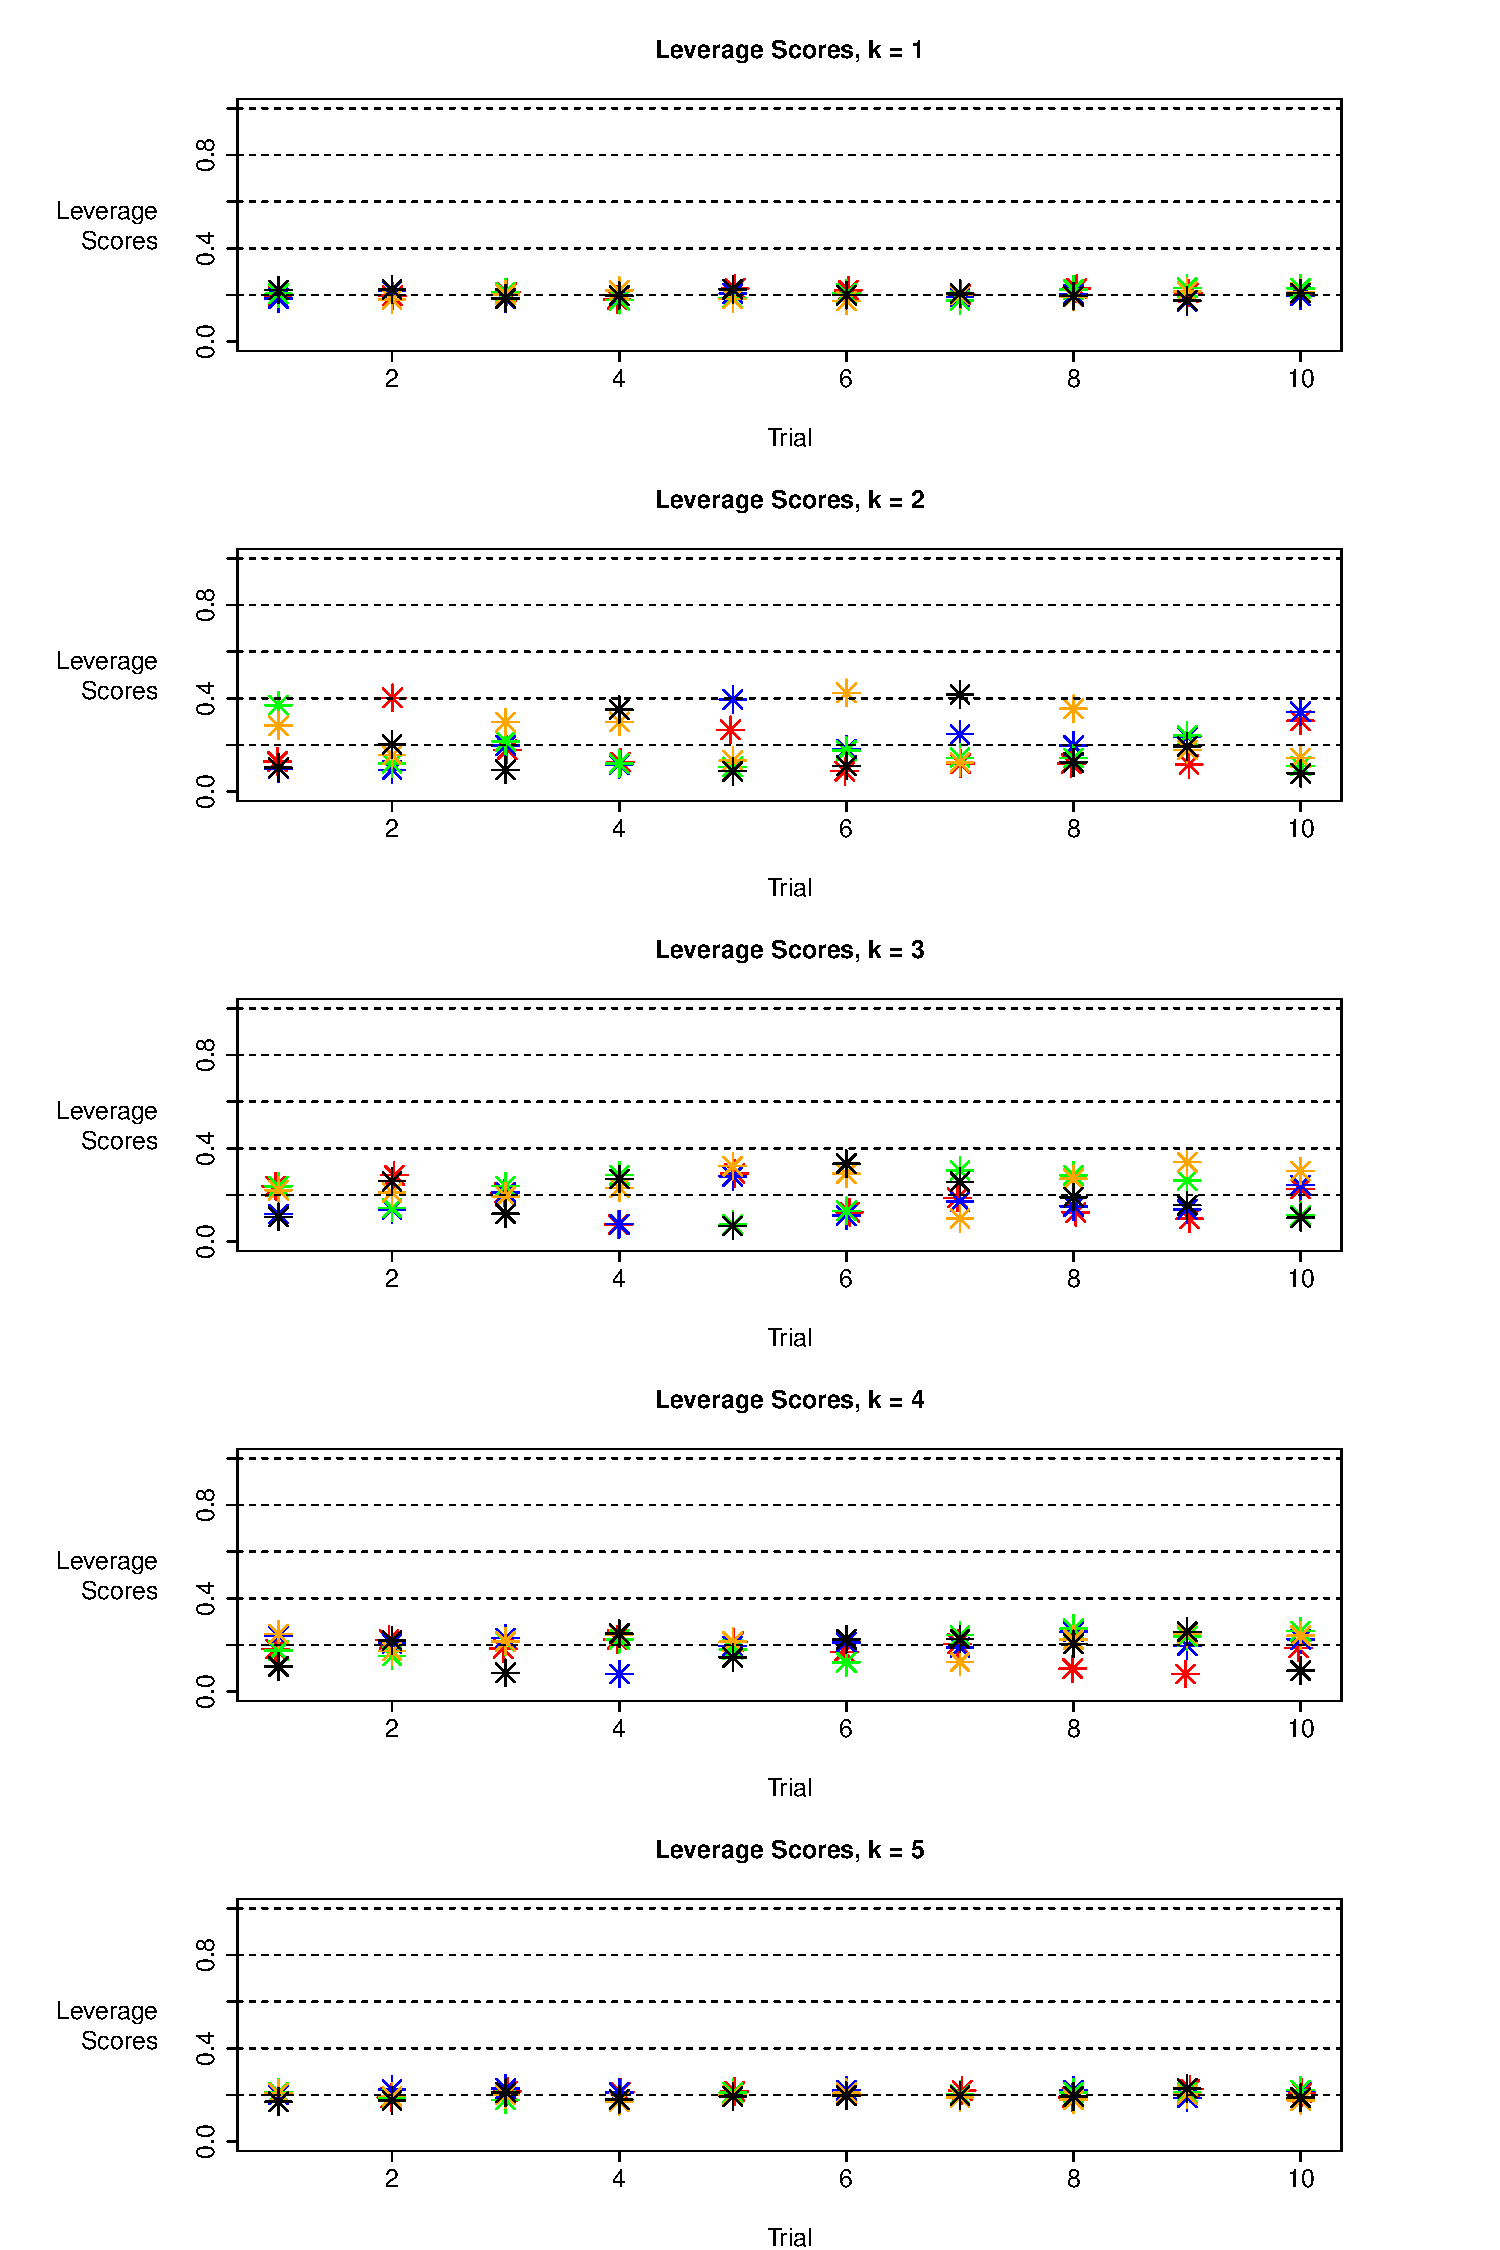
\includegraphics[scale=.6]{./Figures/cs_ex_1/levs.pdf}
\figcaption{The leverage scores of ten $5000 \times 5$ data matrices drawn from our compound symmetric normal distribution.}
\end{center}

\newpage
\begin{center}
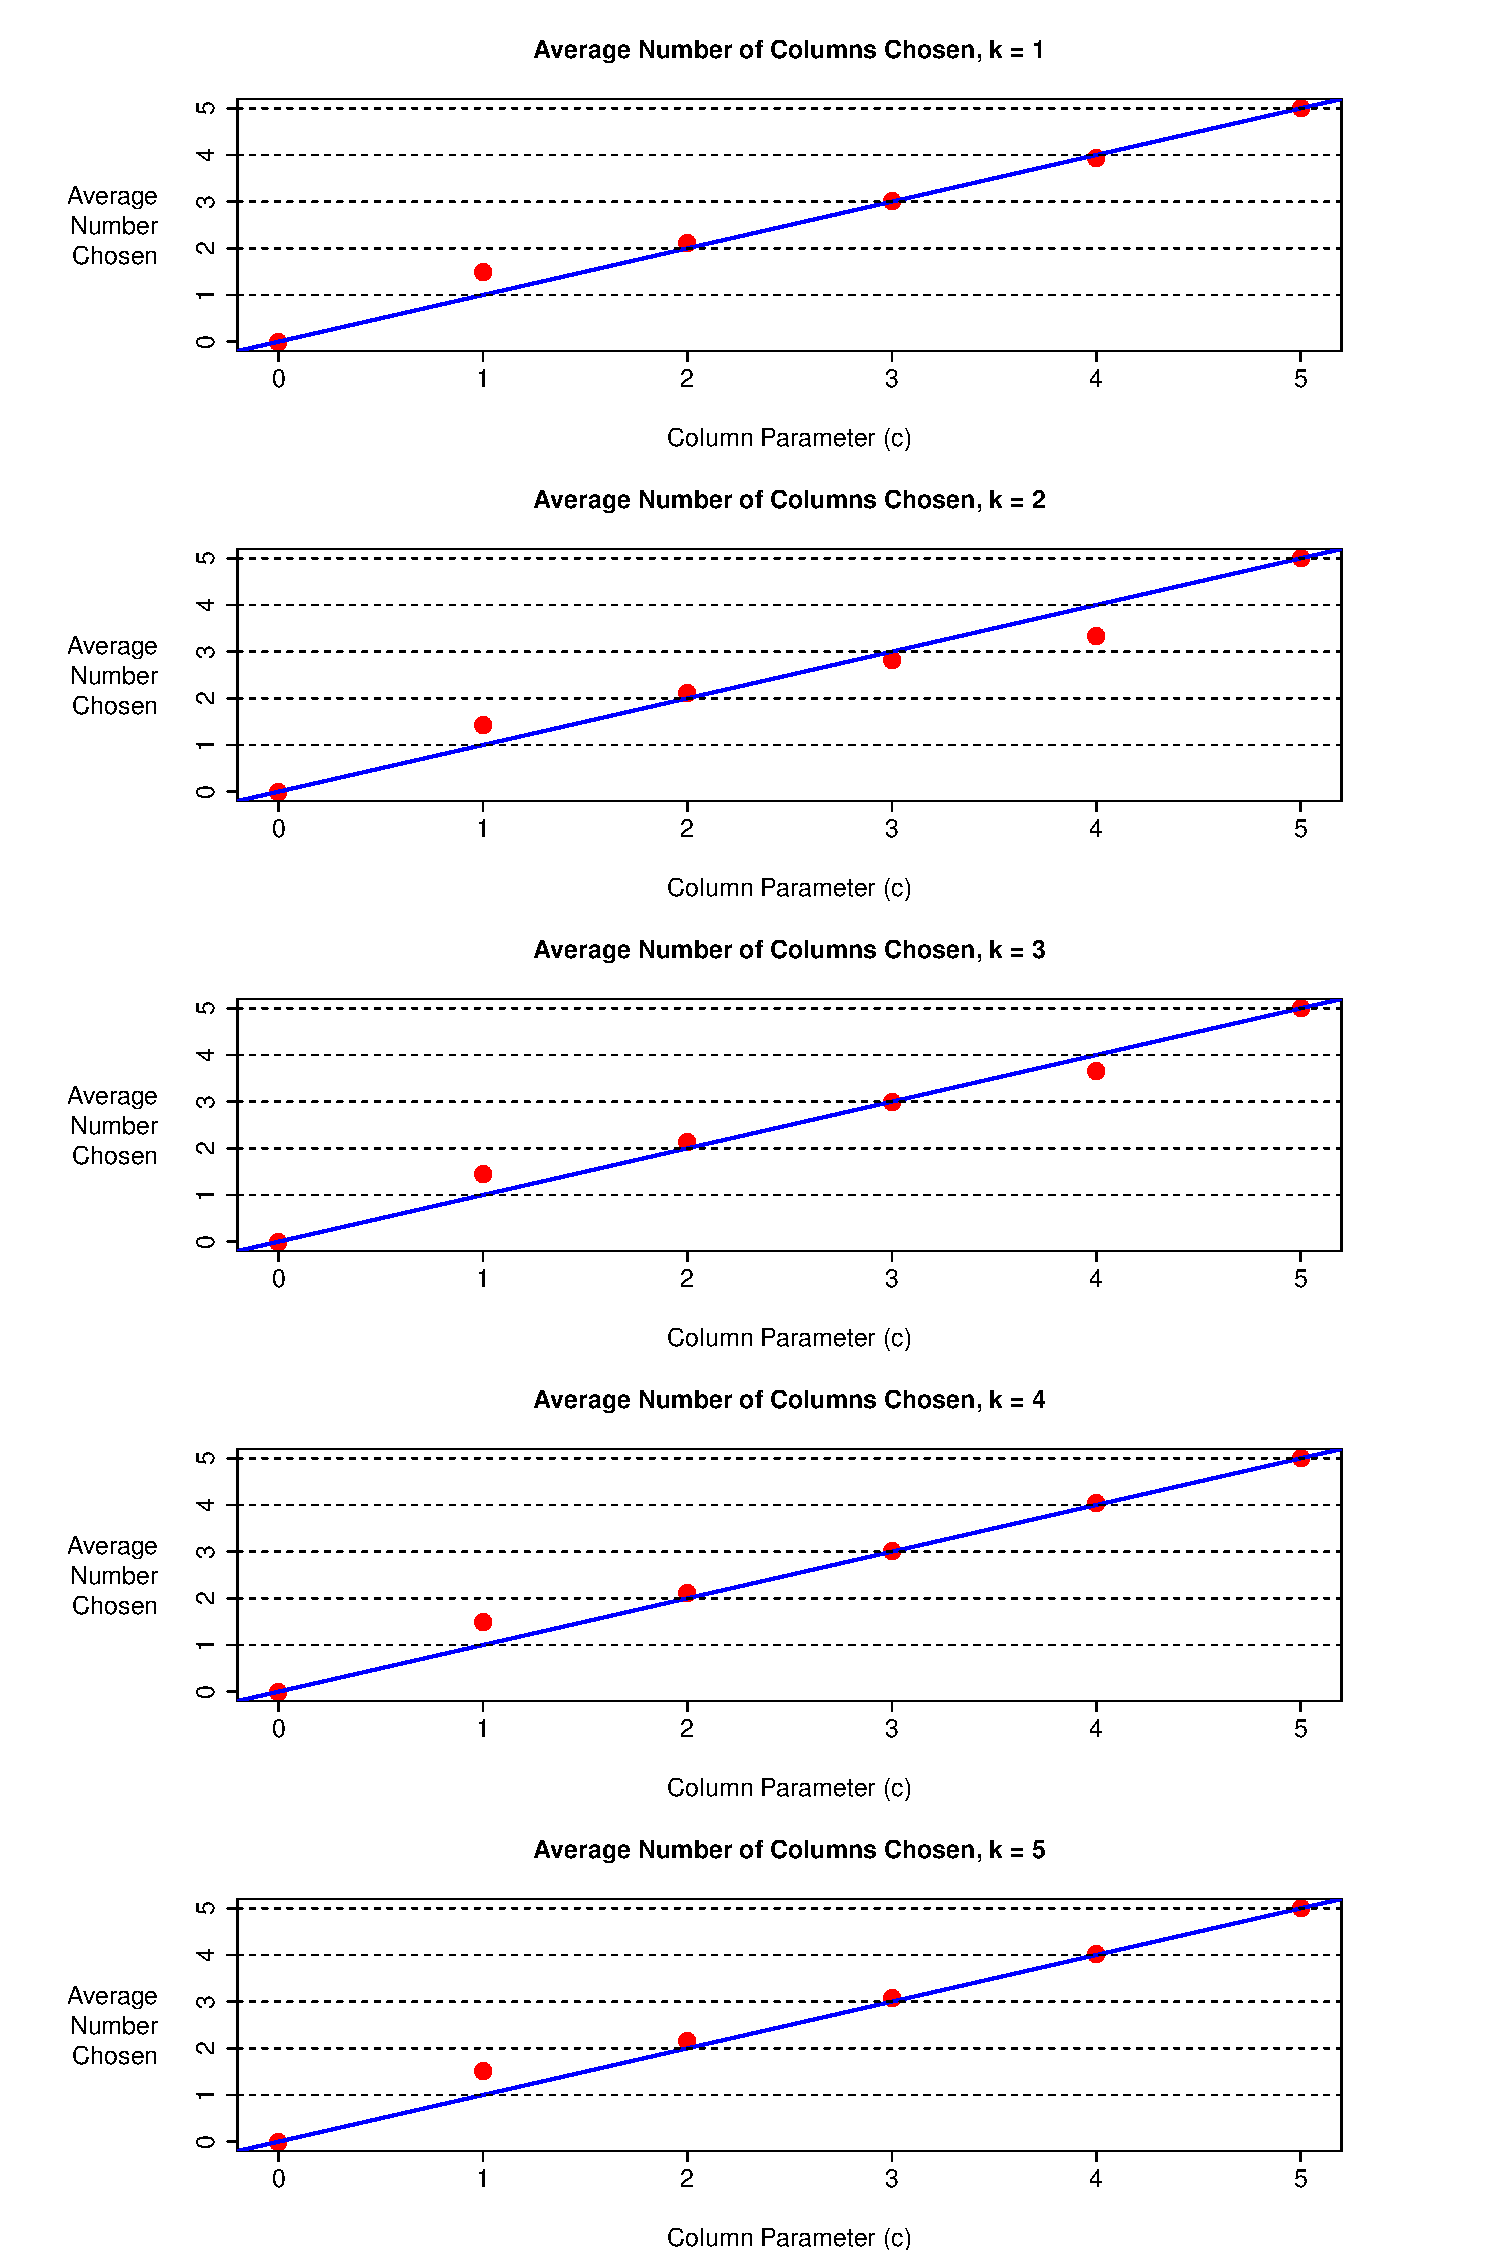
\includegraphics[scale=.6]{./Figures/cs_ex_1/chosen.pdf}
\figcaption{The average ($N = 1000$) number of columns chosen for every permissible value of the rank and column parameters $c$ and $k$. The blue line has slope 1.}
\end{center}



\subsection{Effectiveness}

Now lastly we would like to look at the effectiveness of CUR relative PCA. In Figure 4.21 we plot the average effectiveness score 
$$
e=\frac{||C||_F^2-||D||_F^2}{||X||_F^2}
$$
over $N=1000$ runs of CUR on PCA. Remember that $C$ is the matrix consisting of the columns chosen by CUR and $D$ is the matrix consisting of the principal components constructed by PCA. We plot this value for every permissible value of the rank and column parameters $c$ and $k$. 

\begin{center}
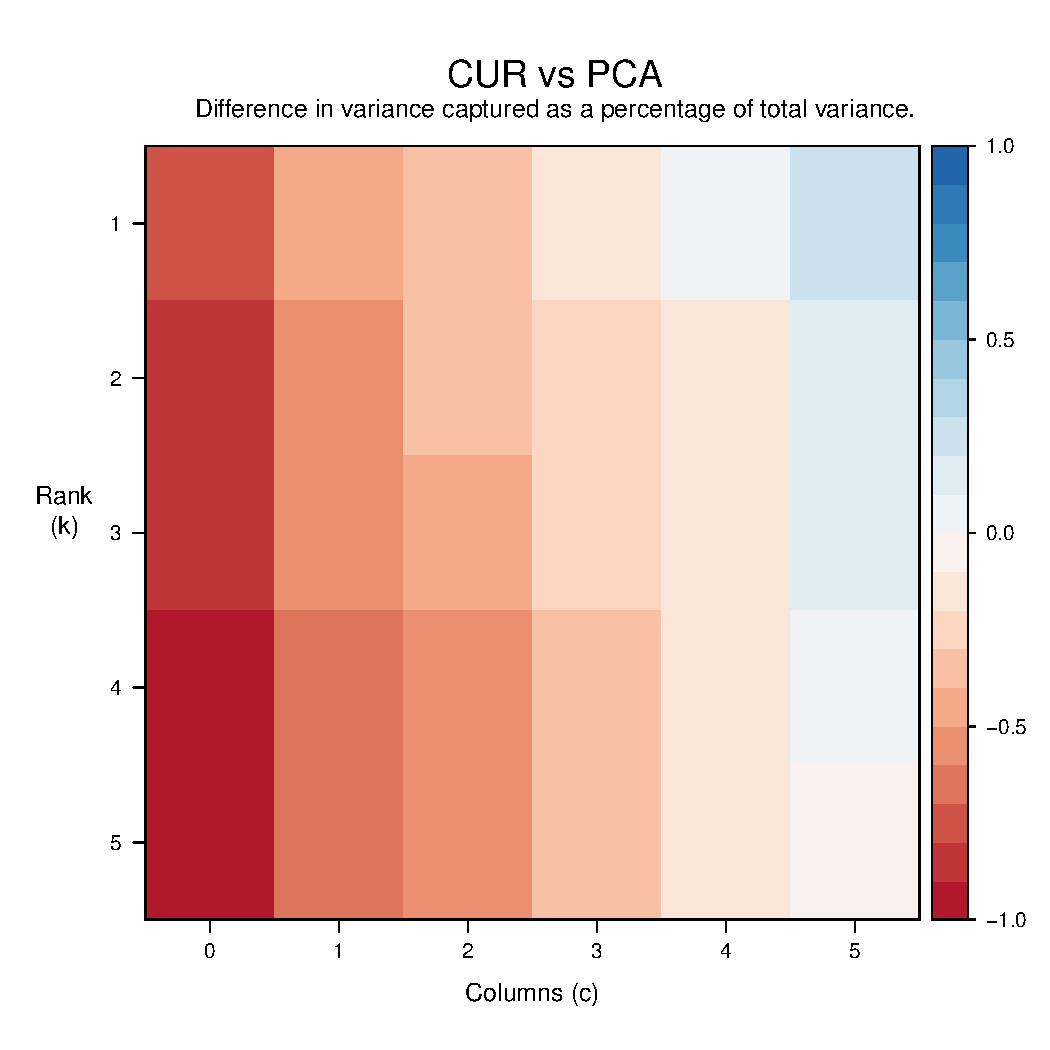
\includegraphics[scale=.63]{./Figures/cs_ex_1/raster.pdf}
\figcaption{A plot of the average (N = 1000) effectiveness value e for each possible value of the rank and column parameters c and k.}
\end{center}

Note that the plot in Figure 4.21 is not very reminiscent of the previous analogous plots in Example 1 and Example 2. The effectiveness score is only positive in the last column where $c=5$. That is, CUR does relatively worse than PCA for almost all of the permissible values of $c$ and $k$. This is not something we have seen before. In our first and second examples there were values of $c$ and $k$ where CUR did relatively better than CUR. However this does not happen for our present example. Almost everywhere CUR does relatively poorly. This behavior is actually not very complicated and we can explore it in much the same manner as in Example 1 and 2. Let us first look at the components of our effectiveness score $e$ 
$$
\frac{||C||_F^2}{||X||_F^2}\text{ and }-\frac{||D||_F^2}{||X||_F^2}
$$
corresponding to the variance captured by CUR and PCA respectively. 

In Figure 4.21 for each value of the rank and column parameters $k$ and $c$ we plot the average percentage of total variance captured by CUR,
$$
\frac{||C||_F^2}{||X||_F^2}
$$
over $N=1000$ runs of CUR on the data. 

\newpage
\begin{center}
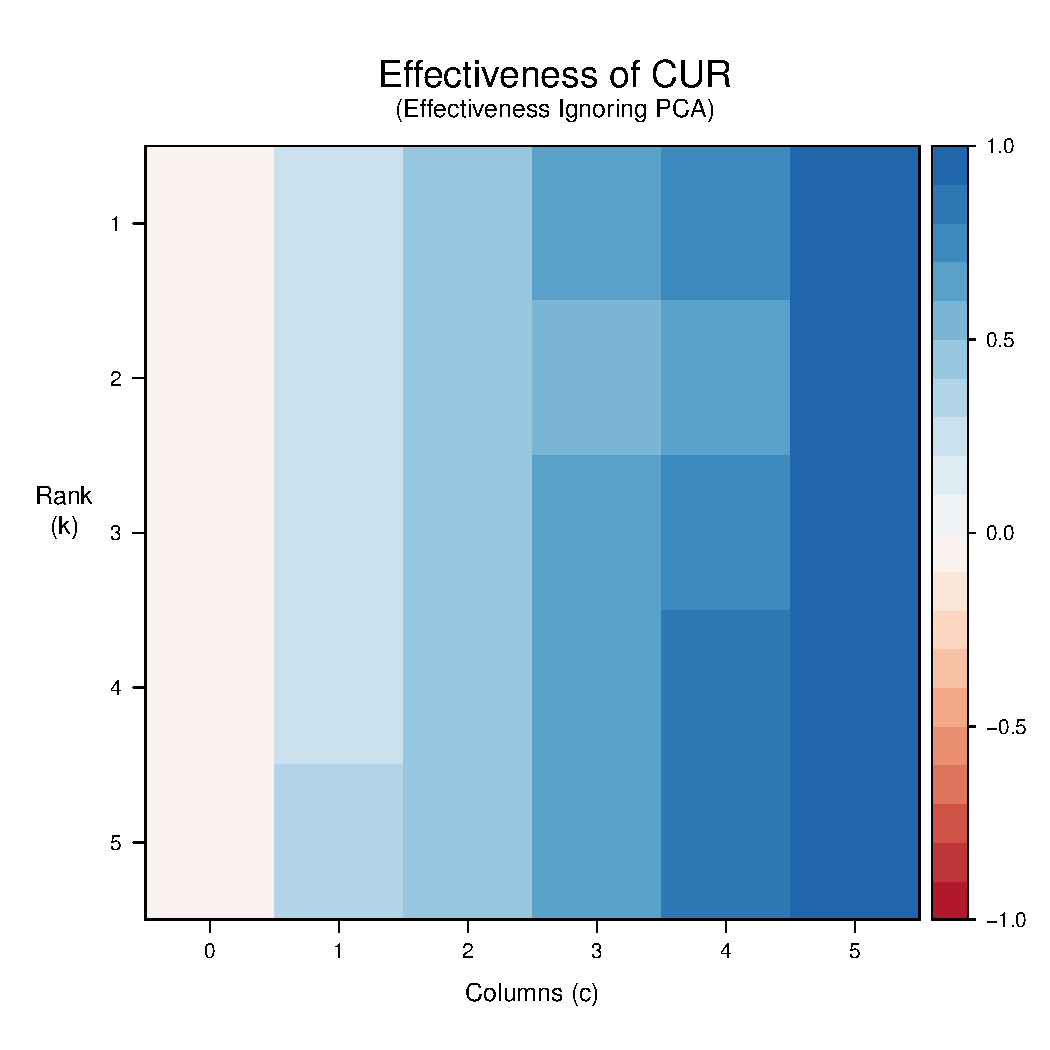
\includegraphics[scale=.5]{./Figures/cs_ex_1/raster_cur.pdf}
\figcaption{A plot of the average percentage of variance captured by CUR ($N=1000$) for each possible value of the rank and column parameters $k$ and $c$.}
\end{center}

The most remarkable feature of Figure 4.22 is that the amount of variance captured by CUR is largely independent of the rank parameter $k$. Indeed Figure 4.22 in our current example looks very reminiscent of Figure 4.6 in Example 1. The similarity occurs for very much the same reason. 

We know that since we are working with a correlation matrix we have that all the variances of the variables (columns) of our data are one. Thus in terms of variance captured there is no reason to privilege one column over another. Furthermore we know from Figure 4.20 that running CUR with a column parameter $c$ will mean we choose about $c$ columns regardless of the rank parameter $k$. Thus the amount of variance captured by CUR is directly related to the number of columns we choose which follows the rank parameter $c$. 

\begin{center}
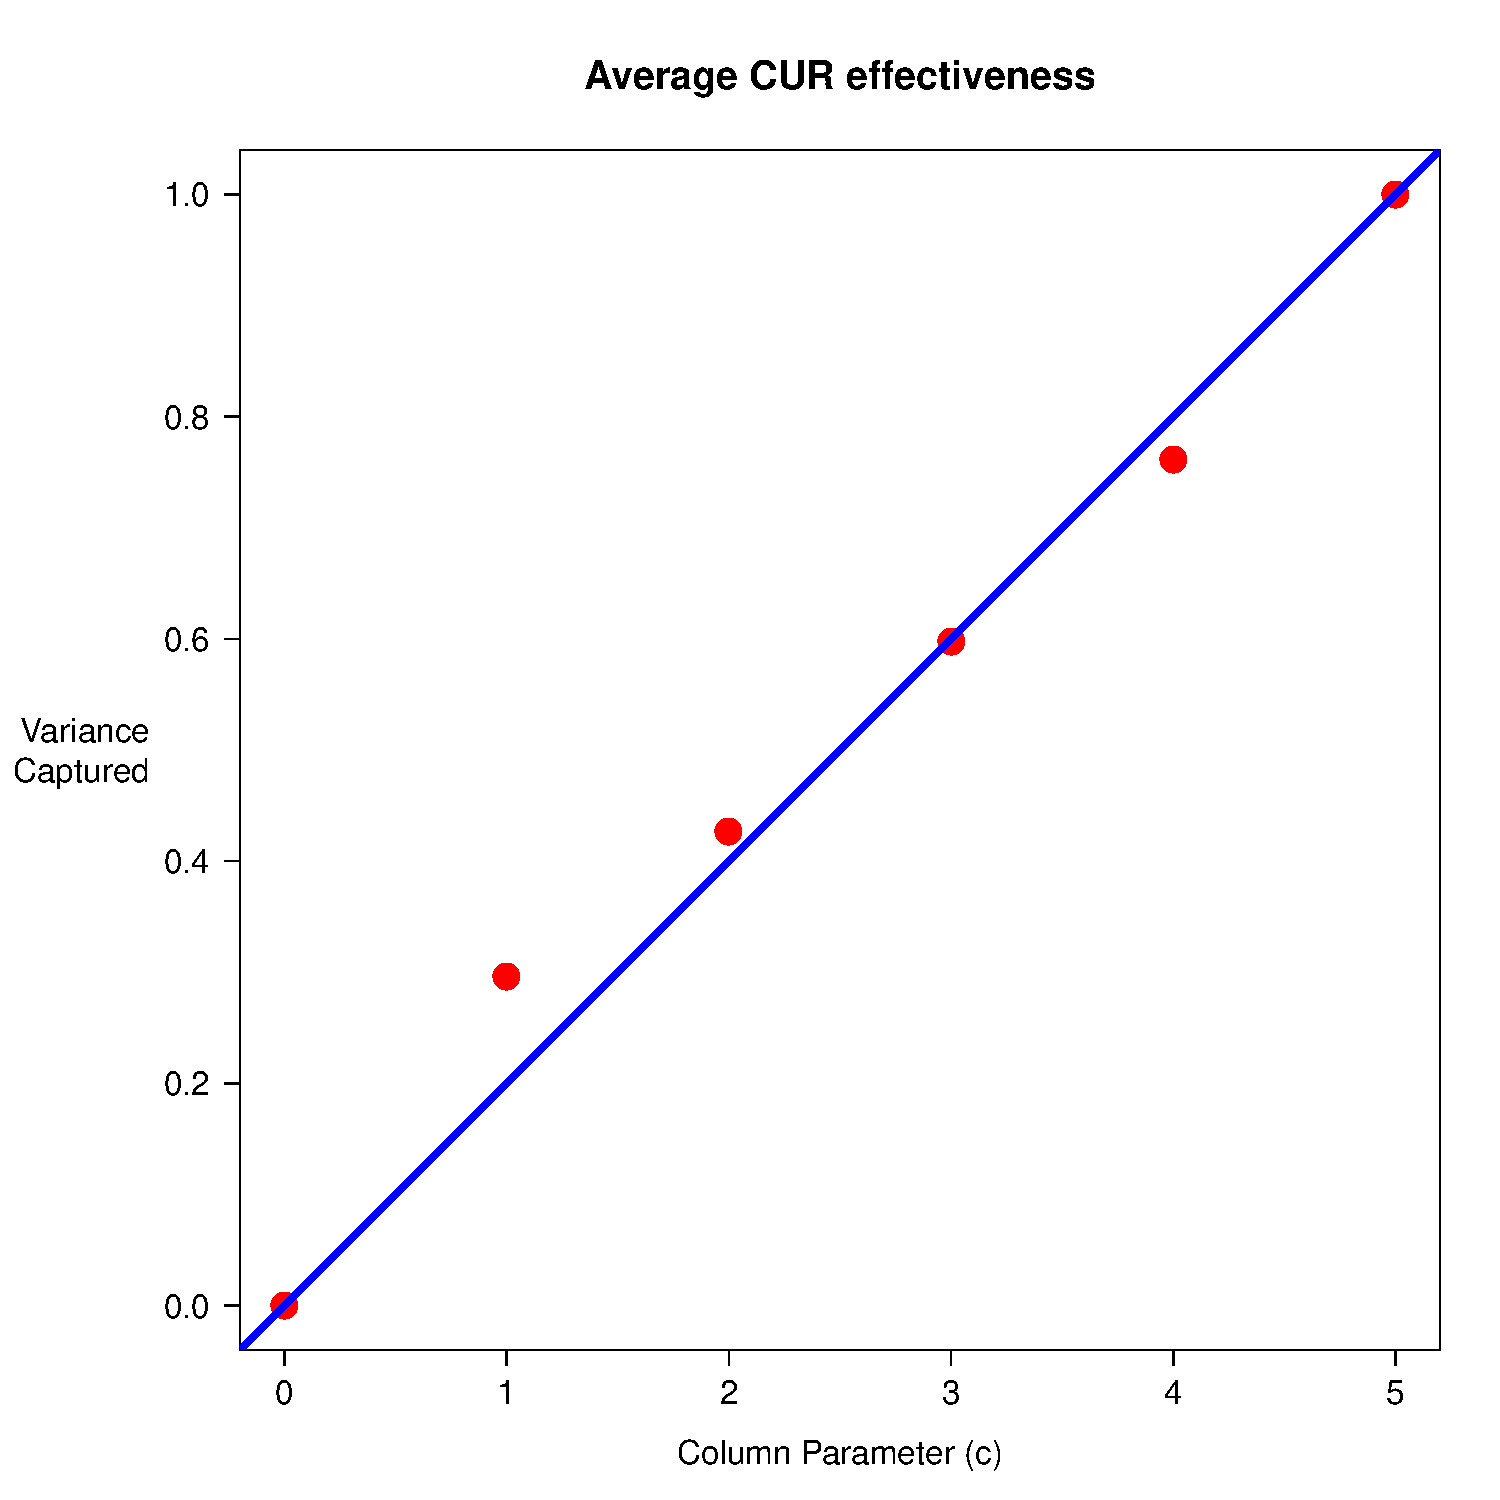
\includegraphics[scale=.3]{./Figures/cs_ex_1/avg_cur_effect.pdf}
\figcaption{A plot of the average percentage of variance captured by CUR ($N=1000$) for each possible value of the rank and column parameters $k$ and $c$. The blue line has a slope of $1/5$.}
\end{center}

In Figure 4.23 we average the average variance captured by CUR across all of the values of $k$. That is, for each column parameter $c$ we average the variance captured by CUR over every possible value of $k$. Note that the relationship is a simple linear one. This is too be expected because each column captures about $1/5$ of the variance and for a rank parameter $c$ we choose about $c$ columns. 

Now to fully explain the behavior we see in Figure 4.21 we plot the average variance captured by PCA in Figure 4.24. That is, for every value of $c$ and $k$ we plot
$$
-\frac{||D||_F^2}{||X||_F^2}
$$
which is the other half of our effectiveness score $e$ and the absolute value of this quantity is the variance captured by PCA. 

\begin{center}
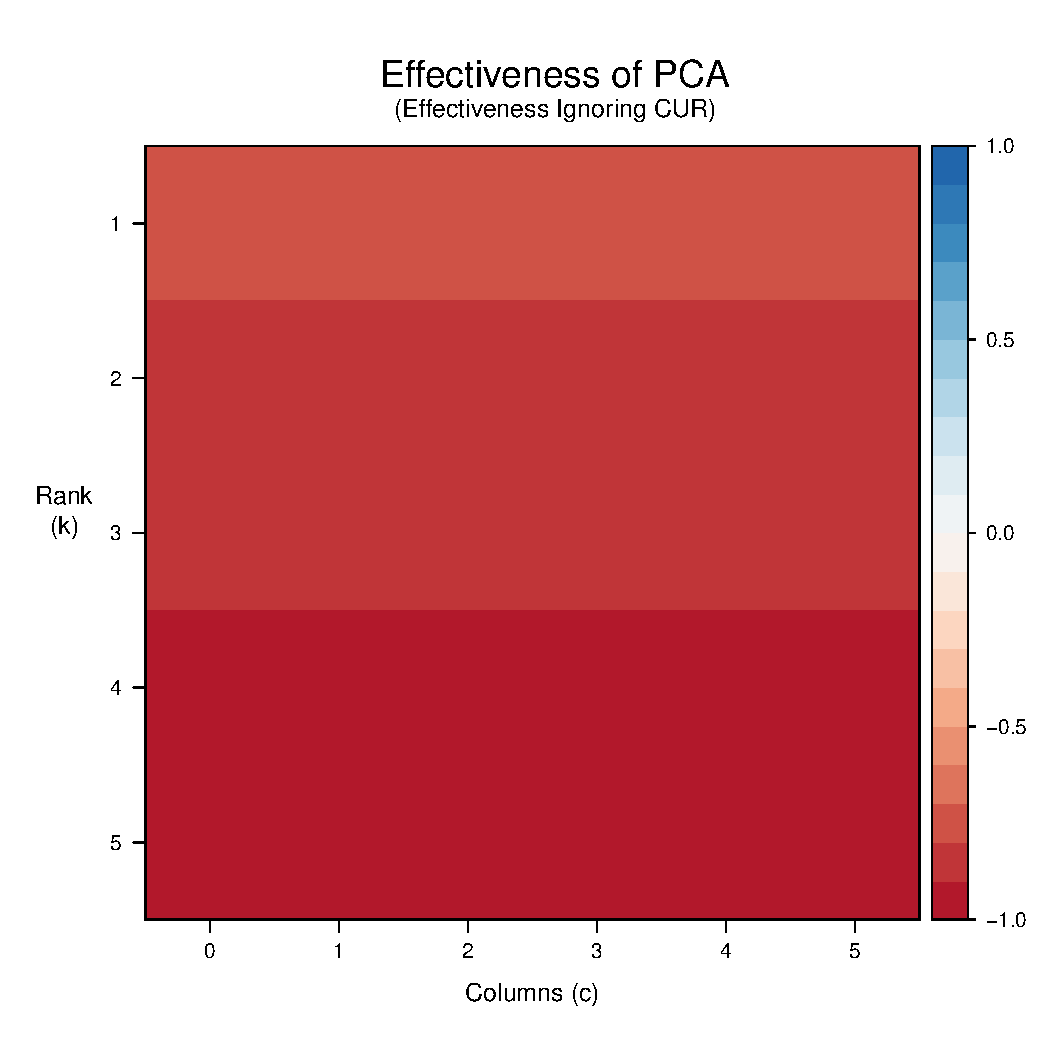
\includegraphics[scale=.63]{./Figures/cs_ex_1/raster_pca.pdf}
\figcaption{A plot of the average percentage of variance captured by PCA ($N=1000$) for each possible value of the rank and column parameters $k$ and $c$.}
\end{center}

What sets this figure apart from previous such plots we have seen is the deep red color of this graph. That is, even for small values of $k$ PCA captures a large amount of variance. This is not too surprising since we know that the first principal component captures
$$
\rho+\frac{1-\rho}{p}
$$
fraction of the total variance. In this example since $p=5$ and $\rho=.7$ then we have that the first principal component captures $76\%$ of the total variance. 

Thus CUR does much worse than PCA for this example. Note that from Figure 4.23 we can see that on average CUR will only capture $76\%$ or more of the variance if $c=5$. This is why the effectiveness score is only positive in Figure 4.21 for $c=5$.

\newpage
\subsection{Conclusion}

A reasonable question to ask is why we chose $\rho=.7$ in this example. Notice that for small values of $\rho$, i.e. as $\rho\rightarrow 0$, the compound symmetric correlation matrix becomes the identity covariance matrix in Example 1. Thus for small values of $\rho$ we expect such compound symmetric correlation matrices to behave similarly to diagonal covariance structure. Furthermore, for a fixed $p$ as $\rho$ increases the percentage of variance captured by the first principal component also increases. After all the amount of variance captured by the first principal component is strictly greater than $\rho$ so long as $\rho \neq 0$.

Thus part of the motivation in choosing $\rho=.7$ is to illustrate a case where CUR does relatively poorly in comparison to PCA. Note that to capture a similar amount of variance CUR must retain many more columns than PCA must retain principal components. Thus, unlike our previous two examples, CUR is generally very poor at reducing the dimensionality of the data. CUR needs to retain $5$ variables to do the job that one principal component may accomplish. This is not too surprising. After all, the subspace that captures the most variance is an average of all the variables. Thus none of the variables can capture this subspace well because it doesn't sit nicely in any of the subspaces spanned by the individual variables. 

The lesson to take away from this example is that having the first few principal components capture a large amount of variance and yet not be aligned well with any of the original variables may cause problems. Unfortunately this is a situation in which we would hope that CUR does well. If the first couple principal components were well aligned with some subset of the original variables then we could say, more or less, that the first principal components are capturing those variables. Thus we would have some sense of how to interpret the principal components.

However CUR should be most useful when the first few principal components not aligned well with the original variable. In this situation it is difficult or impossible to assign a meaning to the principal components. However if the first few principal components capture a large percentage of the variance then CUR balks. We need to retain many more columns than principal components in order to get a comparable result. 


\newpage
\section{Example 4: A Real World Example}

As we did in Example 2 we would like to now add some variance to our data. That is, instead of looking at purely the correlation matrix in our previous example we would like to look at data with a true covariance matrix such that not all the variances are one. 

\subsection{The Data}

For this example we are going to use a real data set in place of the synthetic data we have used previously. To this end we choose a data set called the `crabs' data set from the R package MASS \cite{campbell}. The data description given is the following: 

``The crabs data has 200 rows and 8 columns, describing 5 morphological measurements on 50 crabs each of two color forms and both sexes, of the species Leptograpsus variegatus collected at Fremantle, W. Australia.''

The crabs data measures 8 morphological variables on 200 crabs. There are 100 male crabs and 100 female crabs. Each of these groups is further subdivided into one of two subspecies of either orange or blue crab. There are 50 male and 50 female crabs in each subspecies. The variables measured on the crabs are three categorical variables
\begin{enumerate}
\item species -- either orange or blue
\item sex -- male or female
\item index -- simply a label for each of the crabs
\end{enumerate}
and five continuous variables
\begin{enumerate}
\item frontal lobe size (mm)
\item rear width (mm)
\item carapace length (mm)
\item carapace width (mm)
\item body depth (mm)
\end{enumerate}

For our purposes we will only be using the continuous variables. That is, consider $X$ to be a $200 \times 5$ data matrix where the columns of $X$ correspond respectively to the continuous variables as above. Furthermore we center this data matrix so that the means of the columns are empirically zero. 

Now the correlation matrix associated with $X$ is, to two decimal places,
$$
R=\begin{bmatrix}
1.00& 0.91& 0.98& 0.96& 0.99\\
0.91& 1.00& 0.89& 0.90& 0.89\\
0.98& 0.89& 1.00& 1.00& 0.98\\
0.96& 0.90& 1.00& 1.00& 0.97\\
0.99& 0.89& 0.98& 0.97& 1.00
\end{bmatrix}
$$

The correlations in this matrix are all very large. They are all around $.9$ or larger. Thus if we use the correlation matrix when running CUR or PCA then we are close to being in the same situation as our previous example. We have about equal correlations between all of the variables and this common correlation is high. 

However since all of the measurements on the crabs are in millimeters then there isn't a good reason to scale rescale the variables and work with the correlation matrix instead of the covariance matrix. Thus we will work with the sample covariance matrix and not the sample correlation matrix. Essentially we are then working with data similar to Example 3 except that we are now allowing the variances to be different than one. 

The sample covariance matrix of this data is
$$
S=\begin{bmatrix}
12.22&  8.16& 24.36& 26.55& 11.82\\
 8.16&  6.62& 16.35& 18.24&  7.84\\
24.36& 16.35& 50.68& 55.76& 23.97\\
26.55& 18.24& 55.76& 61.97& 26.09\\
11.82&  7.84& 23.97& 26.09& 11.73
\end{bmatrix}
$$
and so the variances of the variables are $12.22,6.62,50.68,61.97$ and $11.73$ respectively. 

\newpage
\subsection{Eigenvectors and Leverage Scores}

Unlike the previous examples we don't know the underlying population of the crabs data and so we can't talk about the theoretical eigenvectors of the data. Thus, unlike previously, we will not do an analysis of these. 

Instead let us look at the leverage scores for the data. In Figure 4.25 we plot the leverage scores for all five of the variables for each value of $k$. We can see from this figure that the leverage scores are all around $1/5$. They range from about 0 to $2/5$ when $k=1$ and converge quickly to $1/5$ as $k$ approaches $5$. 

\subsection{Columns Chosen}

In Figure 4.26 we plot the average (over $N=1000$ trials) number of columns chosen by the CUR algorithm for each value of $c$ and $k$. While the average number of columns chosen doesn't precisely track with the column parameter $c$ we can see that (especially for larger values of $k$) the number of columns chosen by CUR tracks approximately with the column parameter $c$. 


\newpage
\begin{center}
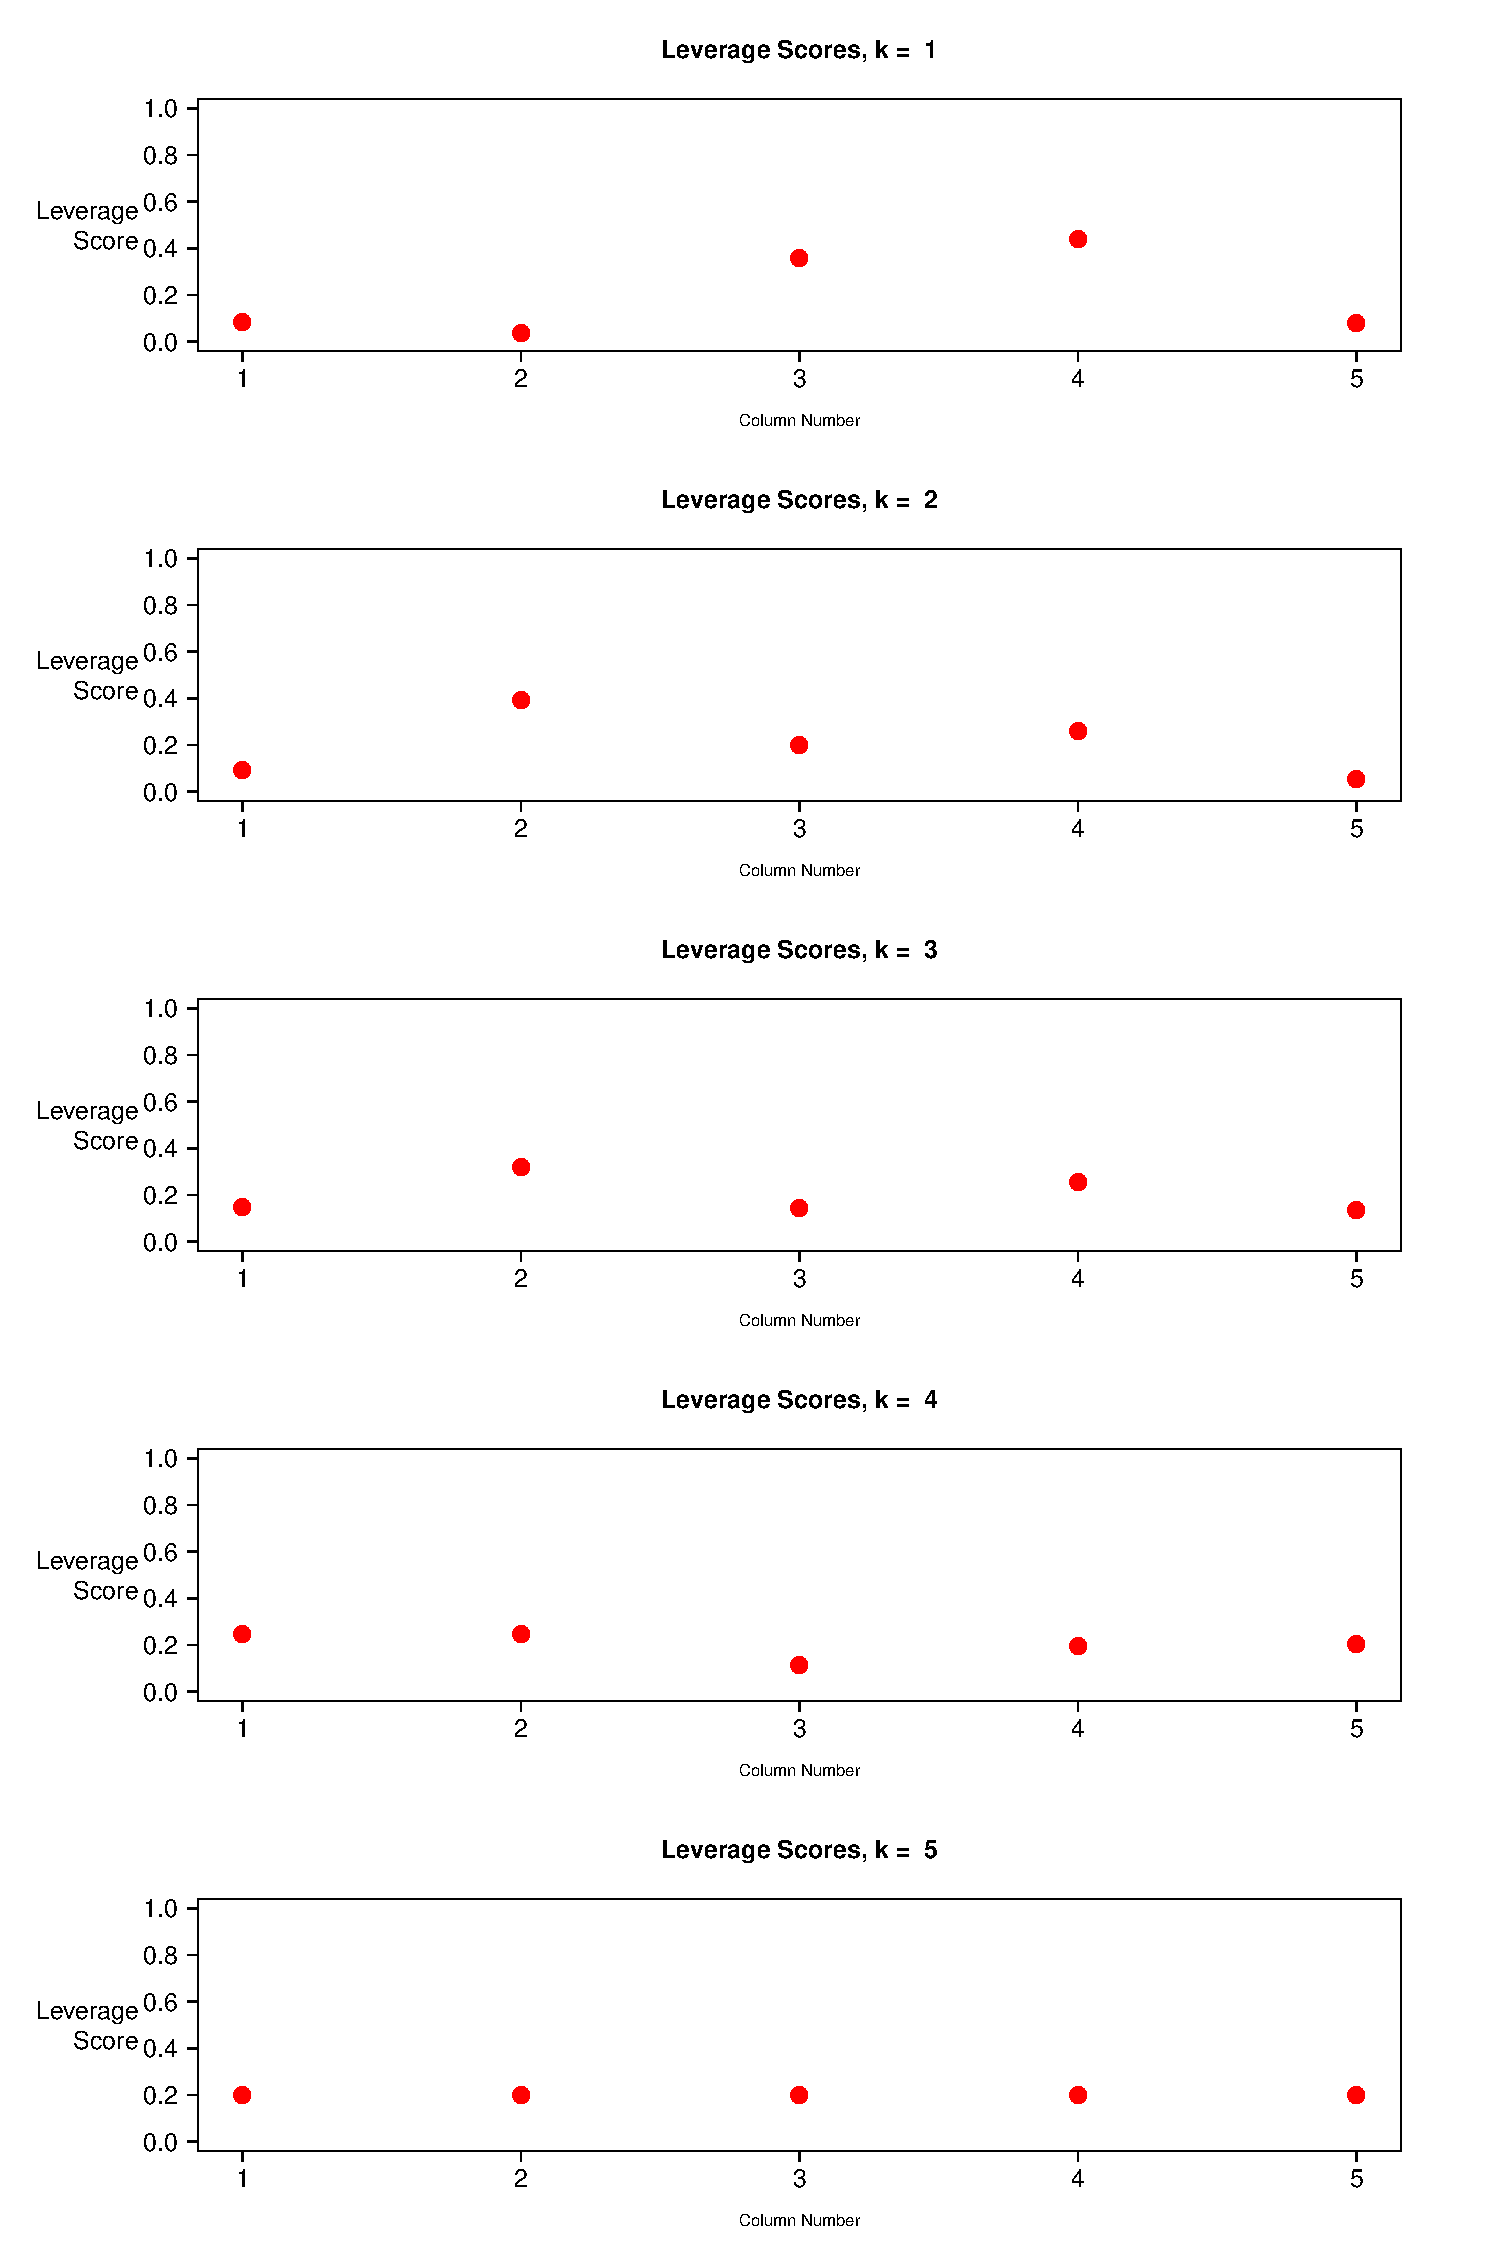
\includegraphics[scale=.63]{./Figures/crabs/levs.pdf}
\figcaption{The leverage scores of the variables over every value of $k=1,\ldots,5$.}
\end{center}

\newpage
\begin{center}
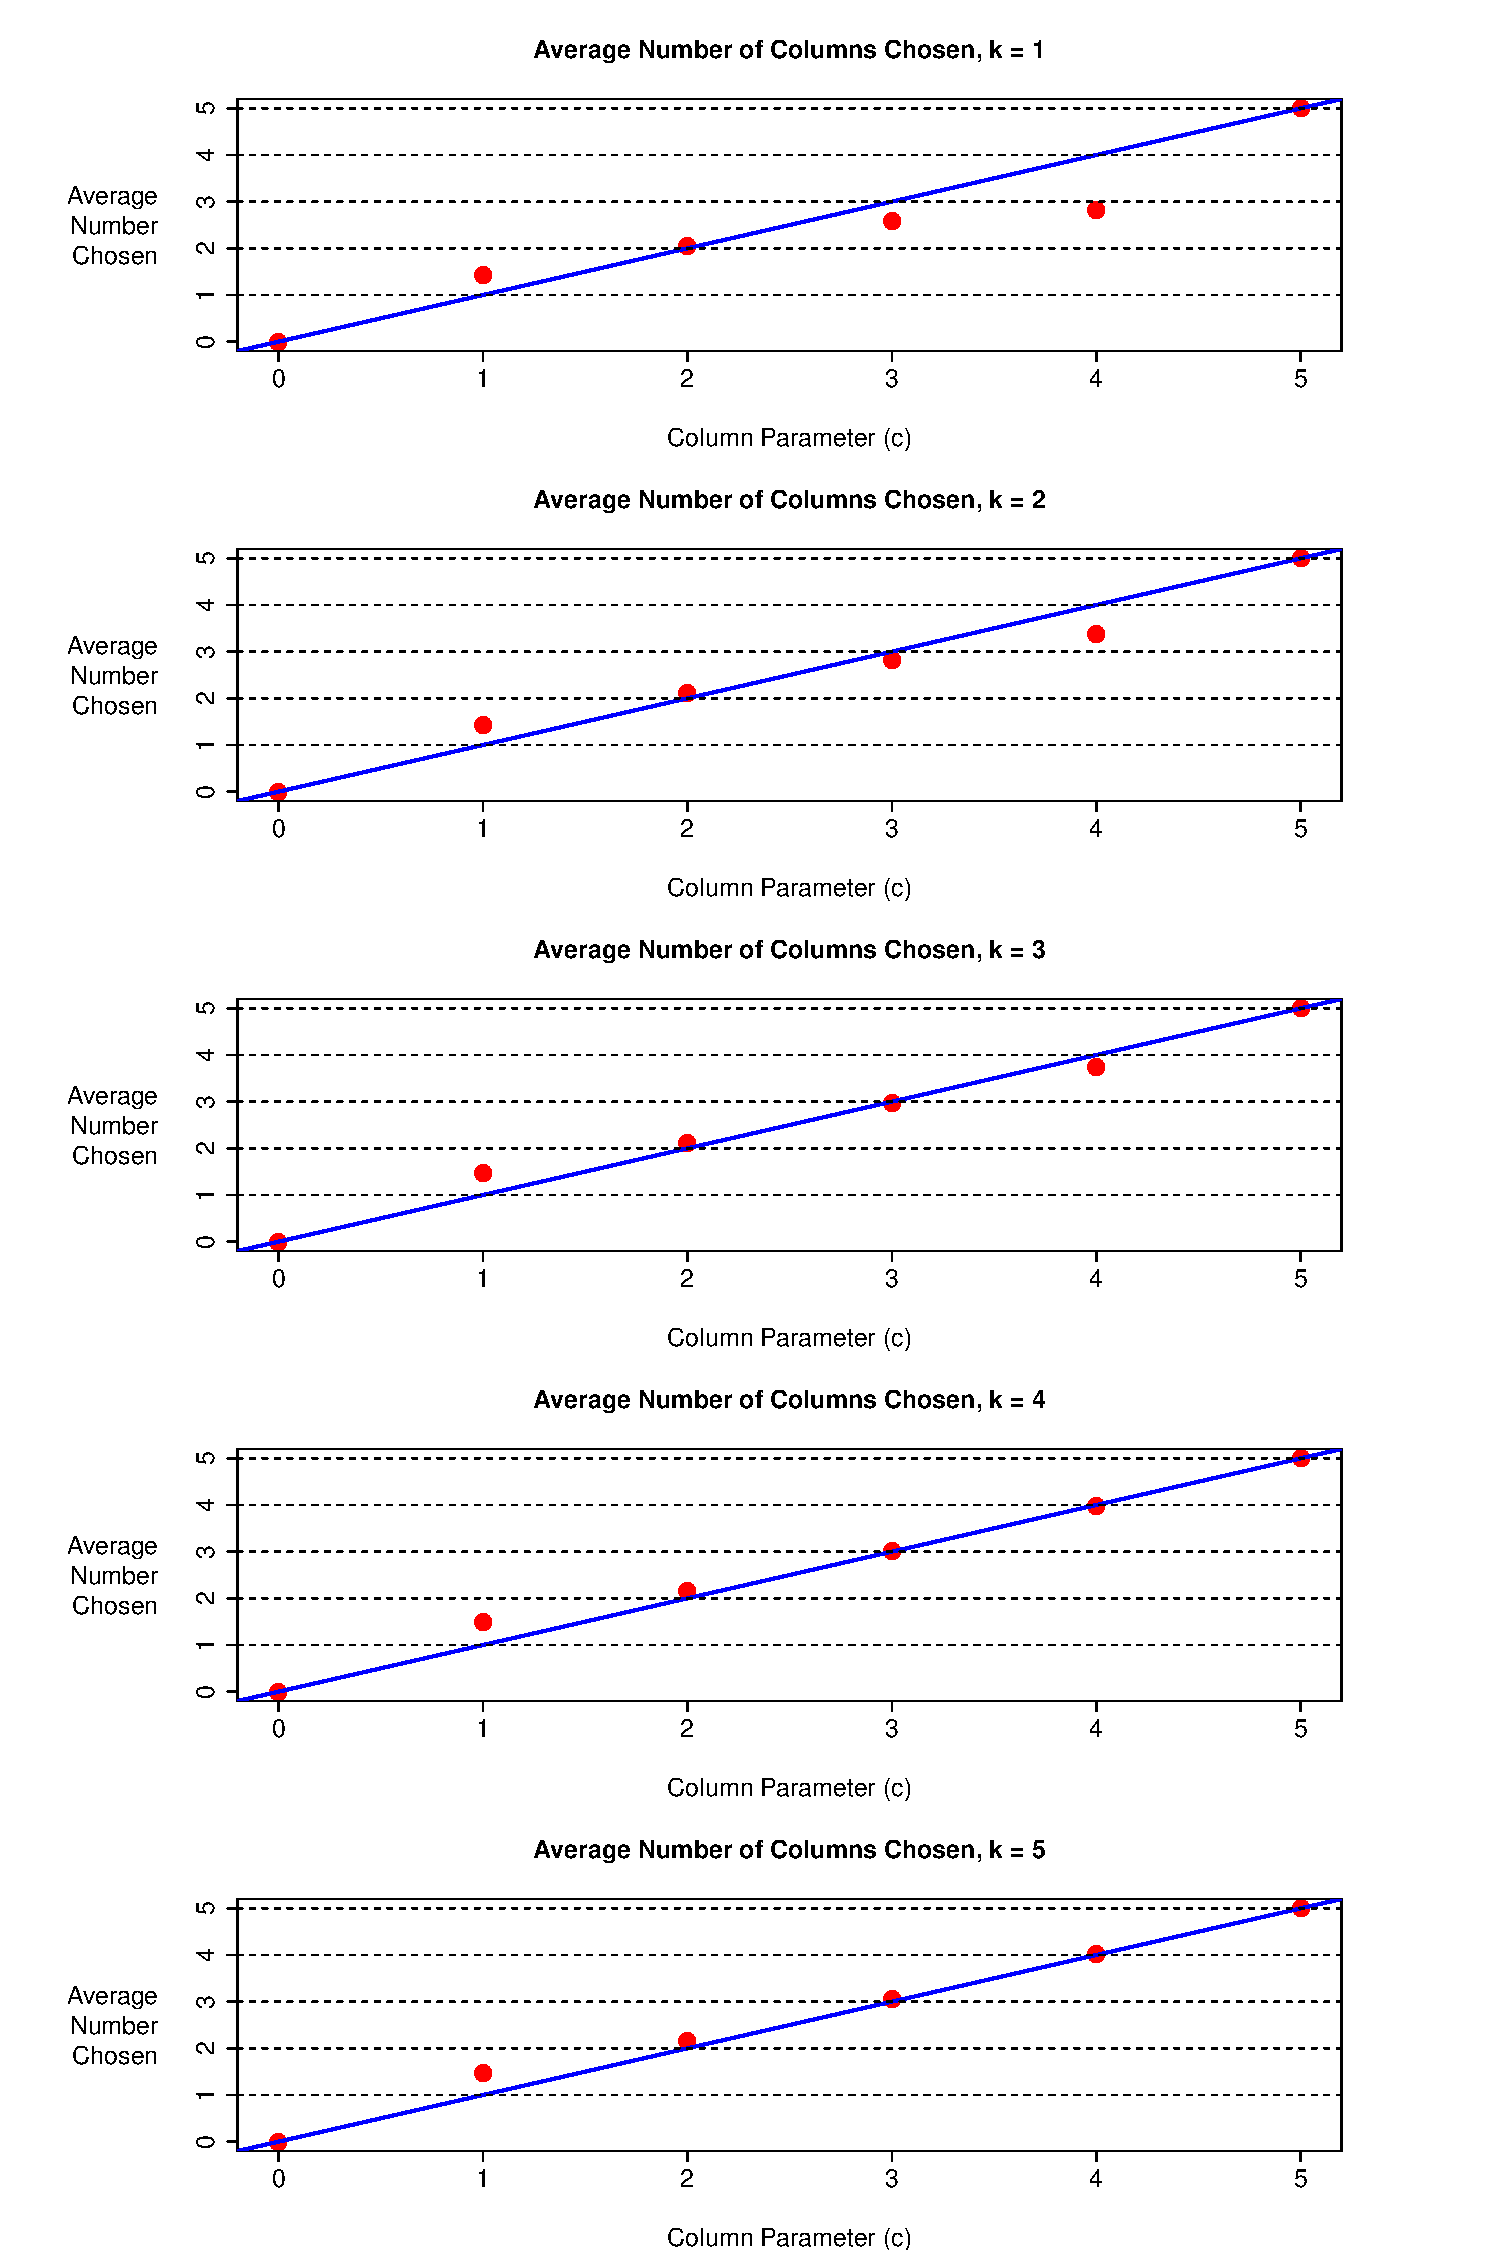
\includegraphics[scale=.63]{./Figures/crabs/chosen.pdf}
\figcaption{The average number of columns chosen by CUR for every value of $c$ and $k$.}
\end{center}


\newpage
\subsection{Effectiveness}

The last thing we want to look at in this example is our effectiveness score of CUR relative to PCA. Thus in Figure 4.27 we plot the average (over $N=1000$) effectiveness score for this data over every value of $c$ and $k$. 

\begin{center}
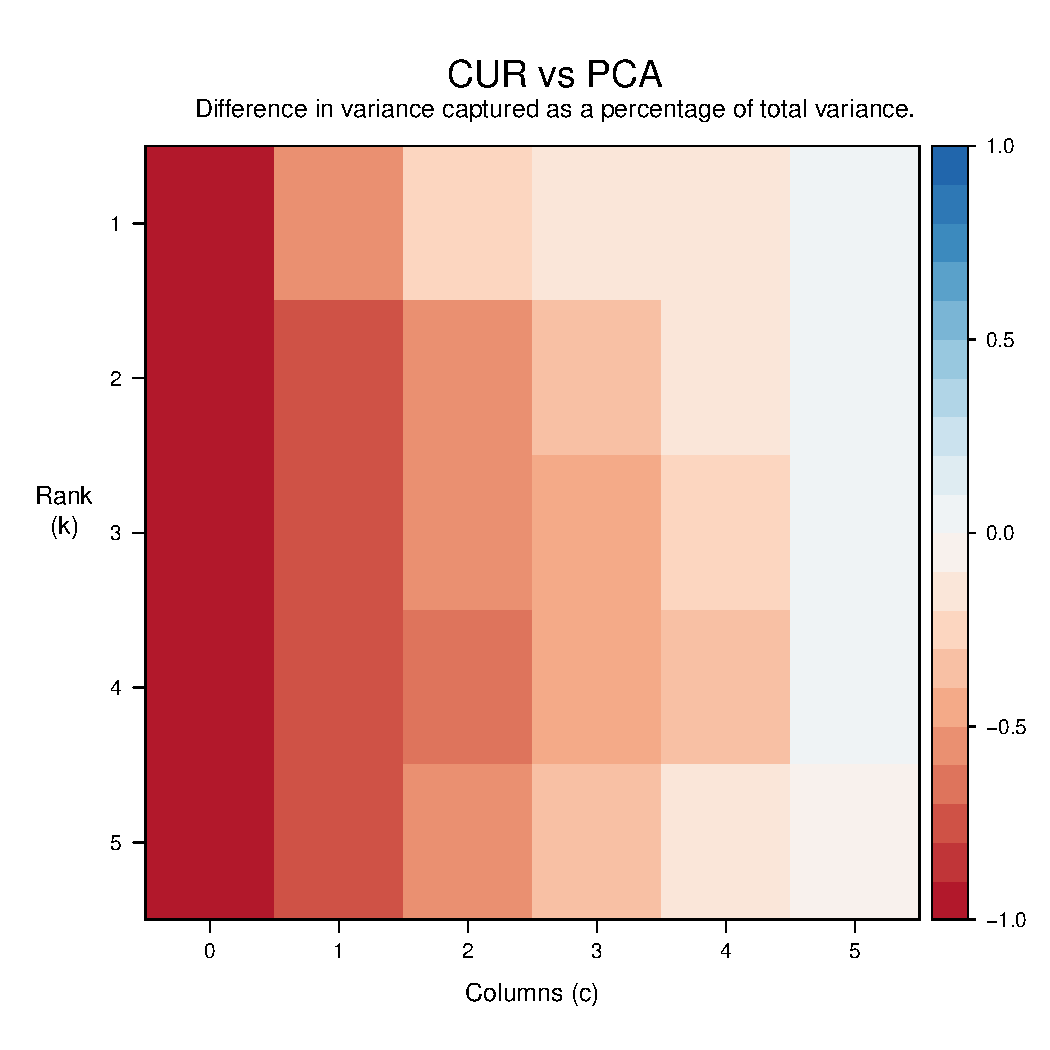
\includegraphics[scale=.63]{./Figures/crabs/raster.pdf}
\figcaption{The average effectiveness score ($N=1000$) for every value of $c$ and $k$.}
\end{center}

We can see in this figure that the effectiveness score is only non-negative when $c=5$ such that we choose every column. This is a reminiscent situation as in Figure 4.21 of Example 3. That is, CUR does poorly for almost all values of $c$ and $k$. This should not be too surprising because the underlying correlation structure is very similar to Example 3.

Consider the plot in Figure 4.28. Notice that PCA captured almost all of the variance even when $k=1$. Let's pretend that we were working with the correlation matrix instead of the covariance matrix as in Example 3. Then as previously discovered the correlation matrix approximately has large and equal correlations among variables. The average correlation off the main diagonal is $\rho=.9466$. Let's pretend that the correlation matrix is actually compound symmetric with a common correlation of $\rho=.9446$. Then the first principal component will capture 
$$
\rho+\frac{1-\rho}{p}=.957
$$
or $95.7\%$ of the variance as per our previous conversation in Example 3. 

While we aren't precisely in the same situation as previously since we are working with the covariance matrix and not the correlation matrix this will not precisely hold. However when we actually calculate the percentage of variance captured by the first principal component we find that it accounts for $98\%$ of the total variance. Thus
 our approximation is not too far off. 
\newpage
\begin{center}
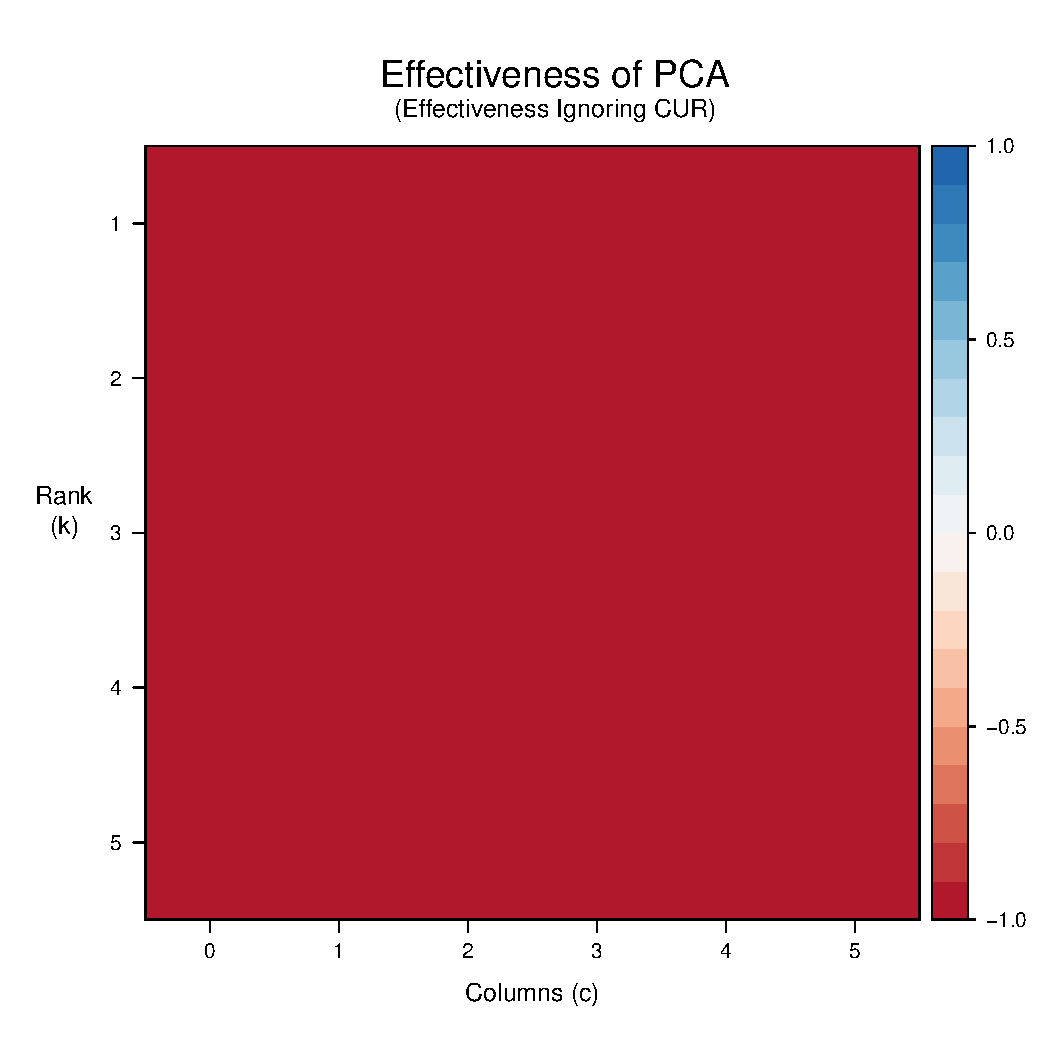
\includegraphics[scale=.63]{./Figures/crabs/pca_raster.pdf}
\figcaption{The average amount of variance captured by CUR ($N=1000$) for every value of $c$ and $k$.}
\end{center}

\subsection{Conclusion}

The data in this example suffers from the same problems as the previous. Examples 3 and 4 are cases where CUR does quite poorly in comparison to PCA. In this example the first principal component captures almost all of the variance of the data. However the first principal component of the data is
$$
PC_1=-0.288\,col(1,X)-0.197\,col(2,X)-0.599\,col(3,X)-0.661\,col(4,X)-0.283\,col(5,X)
$$
which has non-trivial weights for all of the variables. Thus in order to capture the same subspace spanned by this first principal component we really need to choose all of the variables. This is evidenced in Figure 4.27 because we only have a non-negative effectiveness score when we choose all of the variables. 


%%%%%%%%%%%%%%%%%%%%%%
%%%%%%%%%%%%%%%%%%%%%%
%%%%%%%%%%%%%%%%%%%%%%
\addcontentsline{toc}{chapter}{Conclusion}

\chapter*{Conclusion}

In conclusion let us reflect on the goals we set out at the beginning of this paper and see if we may comment on our completion of those goals. 

\vspace{.5cm}
Firstly we wanted to get a sense for how to choose the parameters of the CUR algorithm. There are two parameters of the CUR algorithm. The rank parameter $k$ and the column parameter $c$. We want to use CUR to do something similar to principal components analysis. We have made the argument that if one were to retain $m$ principal components we should set CUR's rank parameter $k$ to be $m$ also. In this case the leverage scores of the columns will be a measure of the similarity of the columns to the first $k$ principal components. Thus, at least in theory, the leverage scores will then help us capture the same information as the first $k$ principal components. 

We have also made the argument that the column parameter $c$ should be equal to the rank parameter $k$ or at least not much different. We have seen both theoretically in Chapter 3 and empirically in Chapter 4 that the column parameter $c$ approximately controls for the number of columns retained by CUR. Consider again running principal components analysis and retaining $k$ principal components. If we want to use CUR to reduce our data to about the same dimension $k$ then we certainly shouldn't pick many more than $k$ columns and thus we shouldn't set $c$ much above $k$. However since we cannot capture more variance than the $k$ principal components retaining less than $k$ columns then we shouldn't set $c$ much below $k$. 

In summary then if we want to use CUR in place of retaining $m$ principal components we should run CUR with $c=m$ and $k=m$. The manner in which one decides how to choose what dimensionality $m$ we should reduce the data to is not a question CUR can answer. However this is no different than PCA. For both PCA and CUR the inspiration of how many dimensions to retain is a question that cannot be answered automatically by the methods. Generally one will look at the eigenvalues of the covariance matrix to make such a decision. 

\vspace{.5cm}

Our second goal for this paper was to determine some of the places where CUR will do well in comparison to PCA and where CUR will do poorly in comparison to PCA. Unsurprisingly the eigen-structure of the covariance matrix has great effect on the performance of CUR. To this end we have two main comments. 

Firstly we have discovered that when our covariance matrix has repeated eigenvalues then the components of the leverage scores coming from the associated eigenvectors will be arbitrary. Thus we should be careful to interpret these leverage scores as defining the importance of the columns. That is not to say that CUR will do poorly in these cases. Indeed CUR did relatively well in Example 1 even though the leverage scores were random. 

Secondly we have discovered that if the first (or first few) principal components capture a large portion of the variance of the data then and the principal components do not align well with the measured variables then CUR will do relatively poorly on this data in comparison to PCA. This follows because PCA is able to capture most of the variance of the data using very few components. Unfortunately in most cases CUR will need to retain a large number of columns in order to capture as much variance as CUR. Thus CUR does poorly in practice because we are not able to reduce the dimensionality well using CUR.

\vspace{.5cm}

While CUR is not a panacea for the interpretability problems of principal components analysis it certainly makes a move in the right direction. Further analysis of the nature of the connection between the eigen-structure of the covariance matrix and the leverage scores for the columns seems to be the best place to start for further analysis. Certainly the CUR algorithm has proven to be useful in some cases even if not so useful in others. The method is quite novel and seems promising and thus further empirical investigations of the kind we have done here seems a worthwhile pursuit. 

\addcontentsline{toc}{chapter}{Bibliography}

\begin{thebibliography}{1}

\bibitem[Lay, 2006]{lay} Lay, David C. Linear algebra and it's applications. 3rd update. Boston: Pearson Education, 2006. Print.

 \bibitem[Rencher, 2002]{rencher} Rencher, Alvin C. . Methods of multivariate analysis. 2nd. Canada: John Wiley and Sons, 2002. Print.

 \bibitem[Johnson and Wichern, 2002]{johnson} Johnson , Richard A., and Dean W. Wichern. Applied multivariate statistical analysis. 5th. Upper Saddle River: Prentice Hall, 2002. Print.

  \bibitem[Mahoney and  Drineas, 2009]{pnas} Mahoney, Michael, and Petros Drineas. ``CUR matrix decompositions for improved data analysis.'' Proceedings of the National Academy of Sciences. 106.3 (2009): 697-702. Print. $<$\href{http://www.pnas.org/content/106/3/697.full}{http://www.pnas.org/content/106/3/697.full}$>$.

  \bibitem[Bodor et al., 2012]{biomed} Bodor, András, István Csabai, Michael Mahoney, and Norbert Solymosi. ``rCUR: an R package for CUR matrix decomposition.'' BMC Bioinformatics. 13.103 (2012). Web. 4 Mar. 2013. $<$\href{http://www.biomedcentral.com/1471-2105/13/103}{http://www.biomedcentral.com/1471-2105/13/103}$>$.

  \bibitem[Hotelling, 1933]{hotelling} Hotelling, Harld. ``Analysis of complex statistical variables into principal components.'' Journal of Educational Psychology. 24.6 (1993): 417-441. Print.

  \bibitem[Pearson, 1901]{pearson} Pearson, Karl. ``On Lines and Planes of Closest Fit to Systems of Points in Space.'' Philosophical Magazine. 2.11 (1901): 559–572. Print.

  \bibitem[Campbell and  Mahon, 1974]{campbell} Campbell, N.A. and Mahon, R.J. (1974) ``A multivariate study of variation in two species of rock crab of genus Leptograpsus.'' Australian Journal of Zoology 22, 417-425. Print.


  \end{thebibliography}



\end{document}
